\documentclass[defaultstyle,11pt]{thesis}

\usepackage{amssymb}		% to get all AMS symbols
\usepackage{graphicx}		% to insert figures
\usepackage{hyperref}		% PDF hyperreferences??
% \usepackage{times}

% self packages
\usepackage{multirow}
\usepackage{url}
\usepackage{amsmath}
\usepackage[ruled,vlined]{algorithm2e}
\usepackage{enumitem}


\hypersetup{
    colorlinks=true,
    linkcolor=blue,
    filecolor=magenta,      
    urlcolor=cyan,
}

%%%%%%%%%%%%   All the preamble material:   %%%%%%%%%%%%

\title{Metadata Matters: Adaptation Methods for Robust Document Classification}

\author{Xiaolei}{Huang}

\otherdegrees{B.E., Central China Normal University, 2013 \\
	      M.S., Chinese Academy of Sciences, 2016 \\
	      M.S., University of Colorado Boulder, 2019}

\degree{Doctor of Philosophy}		%  #1 {long descr.}
	{Ph.D., Information Science}		%  #2 {short descr.}

\dept{Department of}			%  #1 {designation}
	{Information Science}		%  #2 {name}

\advisor{Prof.}				%  #1 {title}
	{Robin Burke}			%  #2 {name}

\reader{Prof. Michael Paul}		%  2nd person to sign thesis
\readerThree{Prof. James H. Martin}		%  3rd person to sign thesis
\readerFour{Prof. Mark Dredze}		%  4th person to sign thesis
\readerFive{Prof. Byron Wallace}		%  5th person to sign thesis


\abstract{  %\OnePageChapter	% because it is very short
% My recent research has demonstrated that metadata has enormous impacts on performances of document classifiers. However, models for \textit{document classification}, the automatic categorization of documents into categories, typically ignore metadata attributes of documents. Metadata, implicitly embedded in documents such as time, gender, age, and location, can have tremendous impacts on the process of building reliable document classifiers. Specifically, we find that classifiers trained by previous year's corpora perform worse on future year's corpora, and similarly, classifiers trained on non-US English (Canadian and British English) corpora has a worse performance on US English corpora, and classifiers show strong gender biases that perform better on male generated documents than females'. Why? Language varies across document metadata: time, gender, age, and location. For example, word senses, usage and context shift over periods of time, and males and females express sentiment differently. Such variations bring both challenges and opportunities to make document classifiers more reliable. 

% % chapter 3 and 4
% We propose to use \textit{domain adaptation} to treat each metadata attribute as domains (e.g., gender domains: male vs. female), aiming to integrate temporal and user demographic factors into document classifiers.
% First, to explore, examine, model and evaluate the language variations into classifiers, we collect and publicize near 1 million labeled documents and 900K annotated metadata entries.\footnote{Data can be accessed by \url{https://cmci.colorado.edu/~mpaul/files/starsem2019_demographics.data.zip}.}
% Next, we proposed multiple solutions to embed the metadata into document representations: feature augmentation, diachronic word embedding and multitask learning. 
% By adapting knowledge of how language varies across the metadata, we can train and learn generalized representations of languages, the metadata-invariant document embeddings. 
% The experiments show our approaches such metadata-invariant document classifiers can generally improve the classification performance.

% % chapter 5
% After showing the effectiveness of the domain adaptation methods, we turn to the NLP ethic and fairness issues caused by language variations. 
% We first collect a hate speech corpora that contains 84K tweets and 64K user entries.
% To obtain domain (gender, age, etc.) invariant document representations, we then propose a feature augmentation method to reduce biases of document classifiers.
% Our hypothesis is that by learning domain invariant document representations, the classifiers can reduce its biases.
% The experiments show the domain adaptation approach can extend to improve fairness in machine learning (unintended bias).

% % chapter 6
% To model both temporal and user demographic factors together, we propose \textit{Dynamic User Embedding} and \textit{Demographic User Embedding} to embed metadata into a single fixed representation by learning user linguistic behaviors.
% By combining user embedding and document classifiers, we can personalize document classifiers and therefore improve document classification performance and further reduce classifier biases. 
% The proposed dynamic and demographic user embedding will have a broader impact on personalized recommendation and language generation beyond building reliable document classifiers.

Metadata, implicitly embedded in documents such as time, gender, age, location, and user history, impacts performances of document classifiers. For example, word sense, usage and context shift over periods of time, and males and females express sentiment differently. However, models for document classification, the automatic categorization of documents into categories, typically ignore metadata attributes of documents. 

In this thesis, we propose to use domain adaptation to treat each metadata attribute as domains (e.g., gender domains: male vs. female), aiming to integrate temporality and user factors into document classifiers. We explore three main directions that adapt metadata into learning representations to build reliable document classifiers. First, we propose the temporality adaptation that explicitly incorporates time into representation learning and modeling processes. Second, we propose a multitask framework using deep neural networks to adapt user demographic factors into document classifiers. We explore the NLP ethic and fairness issues due to the demographic variations and propose a standard feature augmentation method to reduce biases of document classifiers. Finally, we personalize classification models by the user embedding that embeds heterogeneous metadata into a single fixed representation via learning user linguistic behaviors. 

This thesis will also show how those proposed metadata-adapted models can be used in various scientific applications, such as tracking public opinions of public health issues in social media, medical diagnosis and hate speech detection.

}

\dedication[Dedication]{	% NEVER use \OnePageChapter here.
	For the friends and family, who have supported and shaped me on this academic journey. 
	}

\acknowledgements{	\OnePageChapter	% *MUST* BE ONLY ONE PAGE!
    This thesis would not have been done without the support of so many people.
    
    Committee: Michael, Mark, Robin, Jim and Byron.
    
    Collaborators: David Broniatowski, Amelia Jamison, Sandra C. Quinn. 
    
    Summers: Stefan Scherer, Brian Borsari, Lixing Liu, Jason Wu. Jonathan May, Nanyun Peng. 
    Franck Dernoncourt, Walter Chang, Logan Lebanoff and Anthony Michael Colas. Minmin Shen and Angeliki Metallinou (Multimodal machine learning). 
    
    Before PhD: David Chiu, Tingshao Zhu. 
    
    Colleagues: Leysia Palen, Jordan Boyd-Graber, Jed Brubaker, Stephen Voida, Danielle Szafir, Martha Palmer, Amy Voida, Casey Fiesler, Lecia Barker. Linzi Xing, Ben Niu, Ashlynn Daughton, Shudong Hao, Dianna Radpour, Yoshinari Fujinuma. Matt Whitlock, Wendy Norris, Paiheng Xu, Alvin Grissom II, Wei-Lun Harry Chao.
    
    Family: Tingting, Shangming, Qianli.
}

% \IRBprotocol{E927F29.001X}	% optional!

\ToCisShort	% use this only for 1-page Table of Contents

\LoFisShort	% use this only for 1-page Table of Figures
% \emptyLoF	% use this if there is no List of Figures

\LoTisShort	% use this only for 1-page Table of Tables
% \emptyLoT	% use this if there is no List of Tables

%%%%%%%%%%%%%%%%%%%%%%%%%%%%%%%%%%%%%%%%%%%%%%%%%%%%%%%%%%%%%%%%%
%%%%%%%%%%%%%%%       BEGIN DOCUMENT...         %%%%%%%%%%%%%%%%%
%%%%%%%%%%%%%%%%%%%%%%%%%%%%%%%%%%%%%%%%%%%%%%%%%%%%%%%%%%%%%%%%%

\begin{document}


\newtheorem{theorem}{Theorem}


\newcommand{\diff}[2]{\frac{\partial #1}{\partial #2}}
\newcommand{\diffr}[1]{\diff{#1}{r}}
\newcommand{\diffth}[1]{\diff{#1}{\theta}}
\newcommand{\diffz}[1]{\diff{#1}{z}}

\newcommand{\vth}{V_{\theta}}

\newcommand{\twochoices}[2]{\left\{ \begin{array}{lcc}
        \displaystyle #1 \\ \vspace{-10pt} \\
        \displaystyle #2 \end{array} \right. } %}

\newcommand{\threechoices}[3]{\left\{ \begin{array}{lcc}
        #1 \\ #2 \\ #3 \end{array} \right. }    %}

\newcommand{\fourchoices}[4]{\left\{ \begin{array}{lcc}
        #1 \\ #2 \\ #3 \\ #4 \end{array} \right. }      %}

\newcommand{\twovec}[2]{\left(\begin{array}{c} #1 \\ #2 \end{array}\right)}
\newcommand{\threevec}[3]{\left(\begin{array}{c} #1 \\ #2 \\ #3 \end{array}\right)}
\newcommand{\twomatrix}[4]{\left(\begin{array}{cc} #1 & #2 \\ #3 & #4 \end{array}\right)}


\chapter{Introduction}
\label{chp:intro}

% large
Massive annotated text data has been becoming available allows for building document classification models in various domains including news, scientific articles, medical records, political bills, online reviews and social media posts.
Document classifiers automatically classify documents into categories have been widely used for surveillance and diagnosis systems in public health~\cite{lamb2013separating, de2016discovering, huang2019can, zhu2019detecting}, sentiment analysis and user attribute inference in computational social science~\cite{rosenthal2011age, yang2016hierarchical, huang2017exploring, heindorf2019debiasing}, user modeling in personalization~\cite{tang2015learning, wu2016personalized, huang2019neuraluser, pan2019social} and much more. 
The reliability of document classifiers is crucial to the applied domains.


Language varies across document metadata including demographic and temporal factors making document classifiers harder and less likely to generalize. 
However, models for \textit{document classification}, the automatic categorization of documents into categories, typically ignore metadata attributes of documents. 
Metadata, implicitly embedded in documents such as time, author demographic attributes (gender, age, location) and user histories, can impact on building reliable document classifiers.
On the one hand, users are generating new content as well as new ways to express their opinions leading to change in word usage and sense over time, and different demographic groups are using written language as a marker of their own social and community identities causing expression ambiguities.
For instance, the emoji has been reshaping how people express opinions and sentiments over the years~\cite{felbo2017using}, males and females will use the same words to express opposite sentiments~\cite{volkova2013exploring}, and users use different words to express the same sentiment and use the same words to express different meanings~\cite{oba2019modeling}. % examples
On the other hand, document classifiers are generally trained without considering those language variations resulting in instability of classifiers or fairness issues, and even ignore such language variations may cause bias and discrimination to the trained document classifiers: existing research has pointed out failures of existing classifiers because of ignoring the time- and demographic- sensitive attributes in social media data~\cite{gayo2011limits, gayo2013predicting}.
We illustrate how the metadata impacts document classifiers in Figure~\ref{chap1:fig:impact}.
As a result, it is increasingly important to understand, consider and adapt the language variations into document classifiers.


\begin{figure}[htp]
\centering
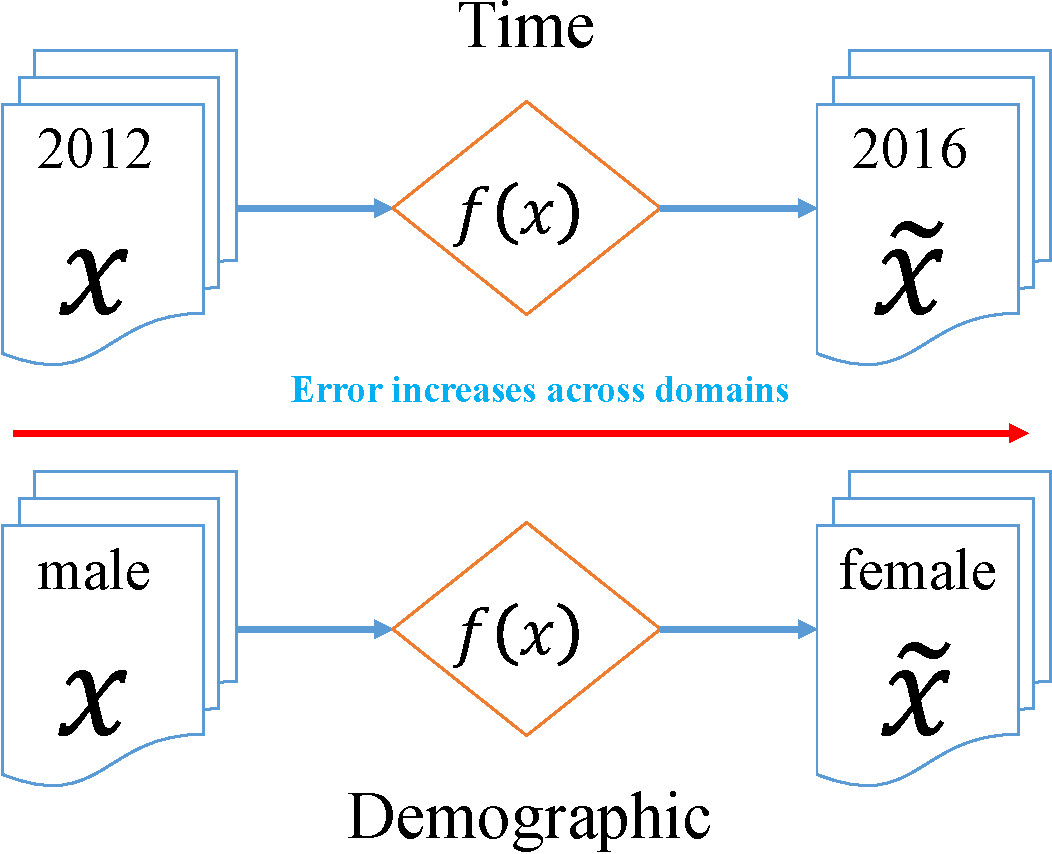
\includegraphics[width=0.55\textwidth]{images/chapter1/metadata_impact.pdf}
\caption{Illustration of how the two metadata will impact on performance of document classifiers. The $\tilde{x}$ indicates the language distributions are different from $x$.}
\label{chap1:fig:impact}
\end{figure}

\section{Contributions and Thesis Overview}

\begin{figure}[htp]
\centering
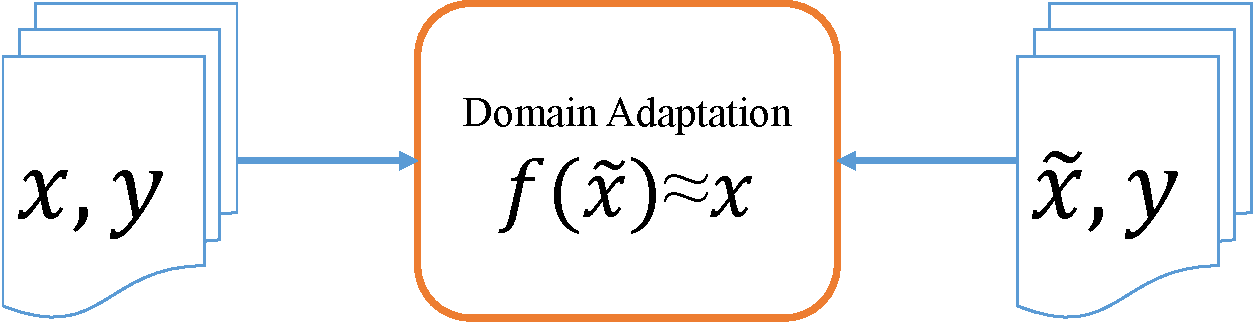
\includegraphics[width=0.55\textwidth]{images/chapter1/da_illu.pdf}
\caption{Illustration of how the domain adaptation works.}
\label{chap1:fig:da}
\end{figure}


In light of these opportunities and challenges, this thesis proposes methods to treat temporality and user factors as domains (2012 vs. 2016 and male vs female domains) and then adapt the metadata into document classifiers using \textit{domain adaptation}.
Domain adaptation is a method in machine learning that learns variations between source and target domains and enables models trained on the source domain can be applied to the target domain. 
Figure~\ref{chap1:fig:da} presents the general idea of how domain adaptation works: to align source and target domains, domain adaptation learns a function to map document representations from the target to the source domain.
The primary contribution of this thesis is to introduce various novel domain adaptation approaches and demonstrate how they can be applied for training more robust and reliable document classifiers towards the metadata.
We propose to treat each variable of individual metadata type as a domain. For example, for the time, we can treat each year or season as a separate domain; for the demographic factors, we can treat male and female as different domains. 

In this thesis, we follow the route towards generalizing and personalizing document classifiers by adapting metadata of documents.
First, we start with backgrounds and applications of domain adaptation.
Second, to integrate temporal and demographic factors into classifiers, this thesis focuses on two types of adaptation: 1) temporality adaptation and 2) user factor adaptation.
We explore the NLP ethic and fairness issues and propose using domain adaptation to reduce biases of document classifiers in the hate speech detection task.
We provide a detailed overview as follows:

\paragraph{Chapter~\ref{chp:background}} summarizes concepts and backgrounds of document classification and domain adaptation. We start with a general discussion of the document classification task. We then provide the important background of domain adaptation in this chapter including an overview of several existing domain adaptation models. The chapter introduces how language varies across the temporality and user factors. Finally, we discuss the impacts of the two factors on both model performance and fairness.

\paragraph{Chapter~\ref{chp:temporality}} illustrates and summarizes the work we have done in the temporality adaptation. We present two temporality adaptation methods via feature augmentation and diachronic word embedding to learn and model the temporal variations in documents. By considering the temporal factor into document classifiers, we show our proposed methods can improve the classification performance. This chapter is based on the published work of \cite{huang2018examining, huang2019neural}.

\paragraph{Chapter~\ref{chp:user}} presents our work on the user factor adaptation. We propose two approaches to adapt user factors under the multitask learning framework. For the user demographic factor, we first introduce and publicize a new dataset with author-level attributes. We then train a classifier by both demographic attributes and document class predictions. We apply the multitask learning framework in training document classifiers aiming to learn domain invariant document representations. Finally, we show the user factor adaptation can generalize and improve classification models. To adapt user latent factors in user history, we train a user embedding model via the multitask learning framework jointly learning both user interests and language usage. We evaluate the user embedding model on an intrinsic task, clustering, and an extrinsic task, document classification. Experiments show that the adaptation method can better model semantic variations of the user language usage. This chapter is based on the published work of \cite{huang2019neuraluser, huang2020user}.

\paragraph{Chapter~\ref{chp:fairness}} illustrates how user factors can cause fairness issues of document classifiers on the author-level attributes (gender, race, age and location). We propose a multilingual hate speech dataset, which each document associates with author-level attributes. The chapter examines classification performance and biases of document classifiers on both English and other languages. We then propose a simple and standard feature augmentation method to reduce biases of document classifiers on the English data. 
This chapter is based on the published work of \cite{huang2020multilingual}.

\paragraph{Chapter~\ref{chp:conclusion}} concludes the thesis with contributions and discussions and suggests future research directions.

\section{Other Research Work}

My research applies machine learning models on solving several health issues, such as suicide ideation analysis, vaccination surveillance, alcoholism diagnosis and COVID-19. 
My work also collects and publicizes new text datasets from online resources. 
However, the massive datasets prevent us from obtaining insights in a short time.
I built and applied document classifiers to extract and summarize information from the millions of documents. 
The following will briefly go through the applications with references.

% applications in public health
Social media sites provide a low-cost and fast accessible way to understand public-health-related opinions and behaviors. \cite{huang2017examining, huang2019can} built several document classifiers and applied them to examine and analyze behavioral patterns regarding influenza vaccinations from Twitter across three dimensions: temporality (by week and month), geography (by US state and region) and demography (by gender).
Suicide is a leading cause of death worldwide. \cite{huang2017exploring} explored the demographic and geographic composition of suicidal users by conducting text analysis of their posts between 2011 and 2016, which were collected in a novel datasets from Sina Weibo, akin to Twitter.
COVID-19 related information has overwhelmed online social media, however, links of information failed to be rated for its credibility. \cite{broniatowski2020covid, huang2020coronavirus} introduced a Twitter dataset of COVID-19 and found a large increase in the proportion of state-sponsored propaganda among the less credible URLs.

Nonetheless, classification models can face challenges in different scenarios, especially in dialogue and multilingual scenarios. \cite{huang2018modeling} explored temporal shifts of user intentions in the alcoholism diagnosis and further demonstrated that temporality can improve classification model performance for medical diagnosis in the dialogue scenario.
Social media provides rich text corpora for different languages, however, the low computational resources of non-English languages prevent mining wider information coverage. 
\cite{huang2019matters} proposed cross-lingual transfer methods that only train sequential classification models on English corpora and apply the models on the other low-resource languages.

\chapter{Background}
\label{chp:background}

This chapter provides the necessary background for this dissertation, including the document classification task, methods of domain adaptation, problem settings of language variations.
This chapter organizes sections as follows:

Section~\ref{chap2:sec:doc_clf} presents a standard pipeline of building document classification models.
I first present steps of document preprocessing and major classification models. 
The document classifiers cover both non-neural and neural types including recent advances of transformer-style models. 
I discuss methods of extracting document representations and standard evaluation metrics for document classifiers. 

Section~\ref{chap2:sec:domain_adpt} introduces important methods and frameworks for the domain adaptation including feature augmentation, multitask learning and domain adversarial training. 
The fundamental methods serve as stepstones for new models that will be proposed in this thesis.

Section~\ref{chap2:sec:time} and Section~\ref{chap2:sec:demographic} demonstrate the challenges of handling language variations across both temporal and demographic factors, which can cause performance drops and prevent model generalizations for the document classification task.
For the temporality, I discuss existing methods that model the temporal factor into neural representations, the diachronic word embedding. 
For the user factor, I present existing methods of adapting user factors. I introduce potential fairness issues of document classifiers caused by user demographic factors. 
The discussions of the language variations and existing methods serve to facilitate introductions of our proposed adaptation methods on both temporal and user factors.


\section{Document Classification}
\label{chap2:sec:doc_clf}
This section focuses on the task of document classification.
The task of document classification aims to assign a document one or more categories by texts, images, or its associated metadata such as author information and timestamp.


\subsection{Preprocessing}
Preprocessing matters for training machine learning models~\cite{camacho2018role,huang2019matters}.
Many tools can help preprocess text documents, such as NLTK~\cite{bird2004nltk}.
The process can have two different levels: text documents and document classes.
Common document preprocessing strategies include lowercase, tokenization, removing stopwords, lemmatization, etc.
For languages like Chinese, we can use segmentation tools~\cite{sun2012jieba} to split a sentence into words.
While most tasks focus on monolingual settings that train and test on the same languages, for cross-lingual settings, translation is an important strategy.
Additionally, preprocessing steps are important for privacy, anonymity and fairness. 
For example for Twitter data, to protect user privacy, we can replace user name, URL and sensitive words with dummy words. 
Research shows that replacing sensitive words in the preprocessing step can significantly reduce the bias of classifiers~\cite{dixon2018measuring}.
To encode the $N$ document labels, we either choose to use sparse categorical classes such as [0, 1, ..., N-1] or one hot encoding which has one 1 and the other N-1 scalars as zeros in a numerical vector. 


\subsection{Traditional Classifiers}

Traditional classifiers including logistic regression and support vector machine (SVM) require extensive labors in designing feature sets.
In this thesis, we mainly use three types of document features: n-gram, topic model, syntax.

\begin{enumerate}
\item \textit{N-gram} extracts token sequences and counts their occurrence. The token sequences have different combinations of lengths, such as unigram, bi-gram, or tri-gram. The count values can be normalized via TF-IDF.  
\item \textit{Topic model}~\cite{blei2003latent} views each document has a distribution over $k$ topics and drive the topic features from each document. The topic feature size is the number of topics, $k$. 
\item \textit{Syntax} can be phonological, morphological, or semantic features. For example, a common feature is a part-of-speech (POS) tag by counting the number of each tag category in every document. 
\end{enumerate}  


We train a supervised classifier by the input feature, $x$, and its associated annotations, $y$. The feature is a D-dimensional vector of numbers to describe the properties of an object, such as length of sentence. The annotations are vectorized to a categorical or nominal variable from some finite set, $y_i \in {1, ..., C}$, where $C$ is the number of document classes. We use the features and labels to train a document classifier, $\hat{y}_i = \theta(X_i)$, by maximizing the log probability, $argmax\sum_{i=1}^nlog P(y_i | x_i; \theta)$, where the $i$ the index of data instance, the $\hat{y}_i$ is the predicted value by the classifier, the $\theta$ refers to the classification function. The training process is that we feed the vectorized training data, $x$, to the classifier $\theta$ to learn the optimum values $w$. Through the model, we can choose the most probable category of the input data.


\subsection{Neural Classifiers}

Neural classifiers have shown their premier performance over traditional classifiers in document classification.
This section first introduces neural representations of words, word embedding.
Then it presents three types of neural models, convolutional neural network (CNN), recurrent neural network (RNN) and bidirectional encoder representations from transformer (BERT).

\subsubsection{Word Embedding}
\label{chap2:subsubsec:emb}

\begin{figure}[t!]
\centering
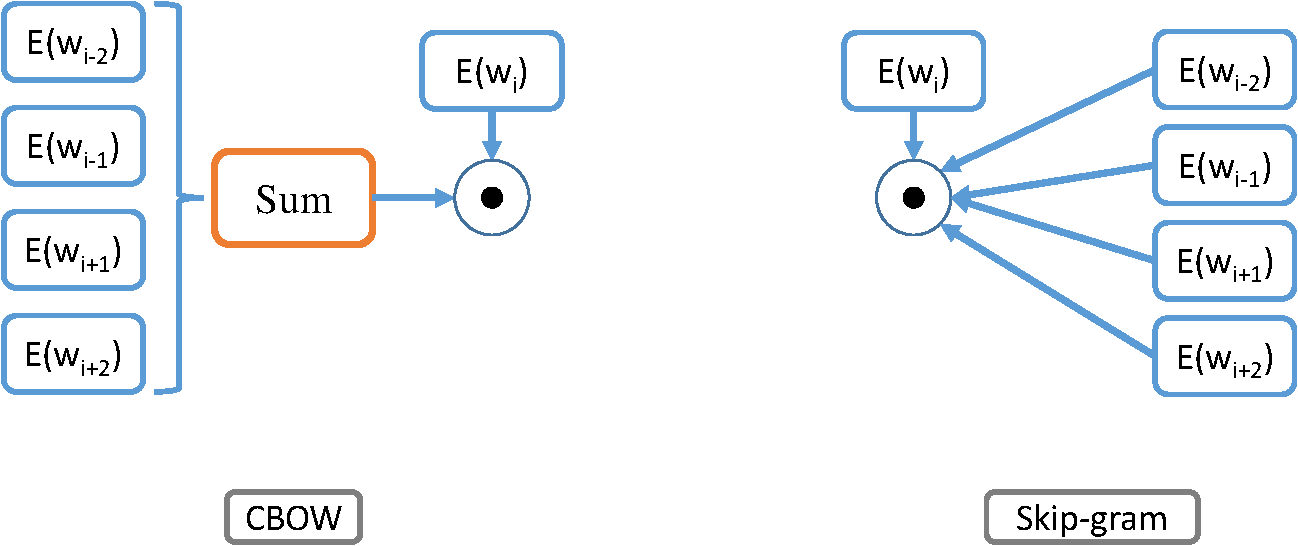
\includegraphics[width=0.85\textwidth]{images/chapter2/word2vec.pdf}
\caption{Two strategies to train word embeddings: CBOW and Skip-gram. Both methods are simple neural models with two layers: hidden layer and output layer. We use the circle to represent dot production.}
\label{chap2:fig:embd}
\end{figure}

The word embedding is to map a word into a fixed-length vector. 
In this section, we will cover methods of building word embeddings from two levels, word and subword. 
We will use them extensively in the following chapters and leave out other methods that are not used in this thesis, such as character embeddings~\cite{zhang2015character}.

\paragraph{Word level} is to encode a token into a fixed dimensional representation~\cite{mikolov2013distributed, pennington2014glove}. 
There are two ways to train word embedding models, Skip-gram and Continuous Bag of Words (CBOW).
We show the details of two training strategies in Figure~\ref{chap2:fig:embd}.

The two methods both first randomly initialize the two embeddings, input ($W$) and output ($U$).
The two embeddings share with the same dimensions $|V| * d$, where $|V|$ is the size of total vocabulary and $d$ is the vector dimension.
For the CBOW, we first generate one hot encoding vector of the context words with the context windows size as $m$ and feed the vector to the input embedding $W$; we can then obtain vector representations of the context words, $W(w_{i-m}), ..., W(w_{i-1}), W(w_{i+1}), ..., W(w_{i+m})$; next, we sum and average the obtained vectors and can get $\hat{w}$; we dot product the $\hat{w}$ with $U$ ($\theta = \hat{w} \cdot U $) and feed the output $\theta$ to a softmax function; we can obtain a predicted probability vector $\hat{y} = softmax(\theta)$ over the whole vocabulary $\hat{y} \in R^{|V|}$; and finally we can optimize the model by categorical cross-entropy $H(\hat{y}, y) = -\sum^{|V|}_{i=1}y_ilog(\hat{y}_i)$.
The key difference between the two methods is that while the CBOW uses the context to predict a word, the Skip-gram predicts the context by a word.\footnote{A detailed comparison can be referred to \url{https://cs224d.stanford.edu/lecture_notes/notes1.pdf}}

However, the softmax and objective functions over the whole vocabulary $V$ consume too much computation, and therefore, we use the \textit{Negative Sampling}~\cite{mikolov2013distributed} to approximate the results and reduce the computational cost.
The negative sampling use one target word and samples $n$ words as negative samples by normalized word frequency $freq^{\frac{3}{4}}$.
By only sampling a small number of words $n \ll |V|$, the negative sampling reduces the computational cost significantly.

% draw the process of skip-gram and cbow
% https://tensorflowkorea.files.wordpress.com/2017/03/cs224n-2017winter-notes-all.pdf

\paragraph{Subword level} represents a word by a couple of subwords, which are sequences of character(s).
The method splits a word into a series of subwords, for example, to represent $where$ by 3-gram characters, we will obtain $whe, her, ere$.
The FastText~\cite{bojanowski2017enriching} appends two positional marks, $<$ and $>$, to the start and end of each word and uses a range of n-gram characters to represent a word. 
Instead of generating a vector for a word, the method initializes an embedding for all subword components.
To represent a word, the method sums and averages representations of all its subwords.
Then the model trains the aggregated word representations to either Skip-gram or CBOW.
The training steps are similar to the word level embedding models shown in Figure~\ref{chap2:fig:embd}.


\subsubsection{CNN}

\begin{figure}[t!]
\centering
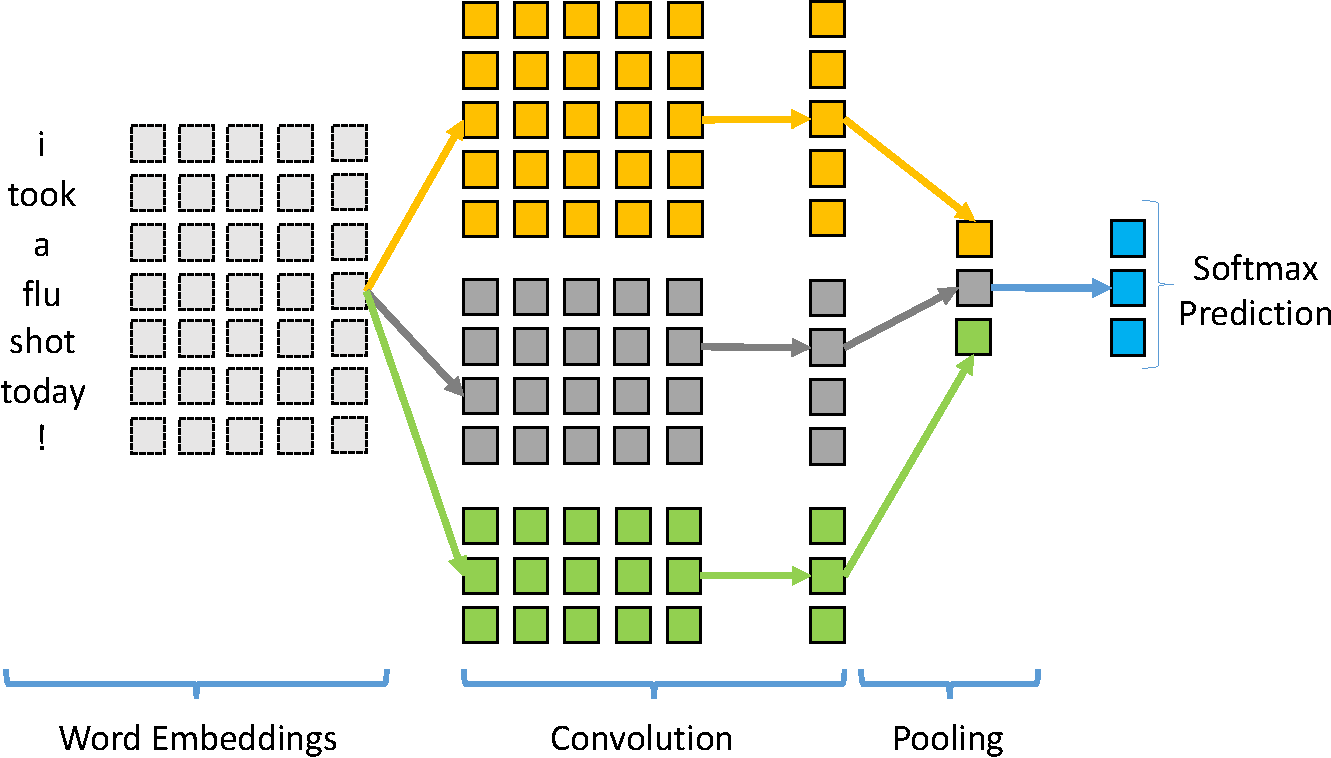
\includegraphics[width=0.90\textwidth]{images/chapter2/cnn.pdf}
\caption{Illustration of CNN model architecture for document classifiers. The simplified architecture follows the existing research work~\cite{kim2014convolutional}. We feed the indices of words to the model. The model initializes pre-trained word embeddings and deploys three different kernel sizes: 5 (yellow), 4 (grey) and 3 (green). We only use 1 filter in each kernel size for simplicity. The model performs a 1-max pooling operation on outputs of the convolution layer. The final softmax layer receives the concatenated outputs from the pooling layer and predicts document categories.}
\label{chap2:fig:cnn}
\end{figure}

Convolutional Neural Network (CNN) has proved its efficiency in document classification~\cite{kim2014convolutional}. 
With the example in Figure~\ref{chap2:fig:cnn}, we will introduce the general principles of CNN document classifiers.
The model first converts a tokenized document to a vector of word indices and pads the vector to a fixed length $n$. 
Then it maps the indices to a lookup table initialized by a pre-trained word embedding, such as Word2vec~\cite{mikolov2013distributed}, GloVe~\cite{pennington2014glove} or FastText~\cite{bojanowski2017enriching} and then obtain a $n*d$ size of document representations, $A$.
The model applies 1D convolution on the document representations $A$ with zero-padding.
The convolution operation has multiple filters with different kernel sizes $h$.
Each filter outputs multiple screenshots, where each screenshot is a sub matrix of $A$, $A[i: i+h] \in R^{h*d}$ and the number of screenshot is $n-h+1$.
Therefore, we can represent the output of a screenshot as $o_i = \sigma(w \cdot A[i:i+h]) + b$, where $i \in [1, n-h+1]$, $\sigma$ is an activation function and $b$ is a bias term.
Multiple screenshots represent generated features of a filter and feed to the pooling layer.
Besides the global max pooling method shown in Figure~\ref{chap2:fig:cnn}, we also have other pooling methods such as average pooling methods.
Finally, the classifier flattens feature representations and feeds the vector to a softmax function for predictions.

While CNN enjoys its parallel processing ability, it only focuses on a limited context and can not retain the long sequential information like the Recurrent Neural Network (RNN)~\cite{goodfellow2016deep}. Next section, I will briefly introduce RNN based classifiers.


\subsubsection{RNN}

\begin{figure}[htp]
\centering
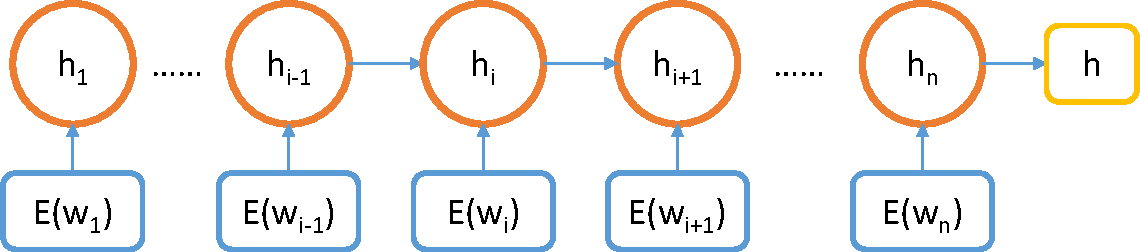
\includegraphics[width=0.85\textwidth]{images/chapter2/rnn.pdf}
\caption{Illustration of RNN model architecture for document classifiers. The RNN model reads a word in each step and recalculates its hidden state by combining the current word and the previous hidden state. The model can have one prediction per step or output its final hidden state.}
\label{chap2:fig:rnn}
\end{figure}

A key advantage of Recurrent Neural Network (RNN) is its ability to learn long dependency sequential information. 
We present a simple RNN model in Figure~\ref{chap2:fig:rnn}.
The model reads the current word $w_t$ in every step $t$ and calculates its current hidden state $h_t$ by $h_t = f(h_{t-1}, w_t; W)$, where the $W$ is the weight of the function $f$.
We can feed the final hidden state $h$ to a softmax function for predictions.

However, the simple RNN can suffer gradients vanish or explosion and hardly capture long dependencies in practice~\cite{pascanu2013difficulty}.
We will introduce two main RNN variants, Long Term Short Memory (LSTM)~\cite{hochreiter1997long} and Gated Recurrent Unit (GRU)~\cite{chung2014empirical}.

\paragraph{LSTM} is one type of RNN models~\cite{hochreiter1997long}. 
It retains more information on contextual dependencies by using structures called \textit{gates}.
The first gate is ``forget gate'' aiming to decide how much information we will throw away from the previous hidden state by 
$$f_t = \theta(W_f \cdot [h_{t-1}, w_t] + b_f)$$
where $\theta$ is sigmoid function,\footnote{The equation of sigmoid function, $\theta(x) = \frac{e^x}{e^x+1}$.} $W_f$ is the weight and $b_f$ is the bias term.
The second gate is ``input gate'' aiming to decide how much information we will use to update the current memory by
$$i_t = \theta(W_i \cdot [h_{t-1}, w_t] + b_i)$$
, where $W_i$ and $b_i$ are the weight and bias term respectively.
Before applying the input gate, we have to calculate the candidate memory value $\title{C}_t$ by $$\title{C}_t = tanh(W_c \cdot [h_{t-1}, w_t] + b_c)$$.
Now, it is time to generate the current memory by using both forget and input gates:
$$C_t = f_t * C_{t-1} + i_t * \title{C}_t$$, which is a weighted combination of previous and new information.
To obtain the output of the current cell, we compute the third gate ``output gate'' by:
$$o_t = \theta(W_o \cdot [h_{t-1}, w_t], b_t)$$.
Finally, we can output the hidden state by $$h_t = o_t * tanh(C_t)$$, where the $tanh$ is the activation function.
We can view the output hidden state as a document representation and build a final prediction layer upon the representation.



\paragraph{GRU} is a simplified version of LSTM in two aspects: fewer number of gates and no memory cell~\cite{chung2014empirical}.
First, it merges the forget and input gates into one gate, ``update gate'' by
$$z_t = \theta(W_z \cdot [h_{t-1}, w_t] + b_z)$$
, where $\theta$ is a sigmoid function, $W$ is the function weight, $h_{t-1}$ is the previous hidden state, $w_t$ is the current input information, and $b$ is the bias term.
Next the GRU combines the cell memory and hidden state into one hidden state by:
$$h_t = (1-z_t) * h_{t-1} + z_t * \tilde{h}_t$$
, where $\tilde{h}_t = tanh(W_h \cdot [r_t * h_{t-1}, w_t])$.
The $r_t$ refers to a ``reset gate'' and calculates the gate by $r_t = \theta(W_r \cdot [h_{t-1}, w_t])$.
The reset gate decides to retain how much previous information.
Existing empirical research finds that the GRU shows a similar performance with the LSTM while reduces computational costs because of the simplified architecture~\cite{chung2014empirical}.


\subsubsection{BERT} 
Bidirectional Encoder Representations from Transformer (BERT)~\cite{devlin2019bert} is a Transformer~\cite{vaswani2017attention} style language model learning rich semantic information on large unlabeled corpora.
The model has two primary bases, 12 and 24 layers, which contains 110M and 340M parameters respectively.
Outputs of the model can be feature representations of documents.
We can then feed the representations to different downstream tasks.
The pre-trained model has been widely applied in several downstream tasks, such as sentiment analysis, question answering, etc.

% how it pretrained: pretraining tasks
The language model learns semantic information from two pre-training tasks, masked language modeling (Masked LM) and next sentence prediction (NSP). 
For the Masked LM, the model randomly replaces 15\% of tokens in a document by a special token [MASK] and then use the encoded token representations to predict the masked tokens.
For the NSP, the model is to predict a binary relationship between two sentences that whether the second sentence follows the first sentence.
To encode a token, BERT represents each token from three aspects: word (token), segment and position embeddings.
The word embedding is similar to the Section~\ref{chap2:subsubsec:emb}, the segment embedding indicates a token belongs to the first segmentation or the second one, and the position embedding encodes sequential information of tokens.
BERT sums the three types of embeddings and forwards the representations to several layers of transformers.
Outputs of the final layer are usually for downstream tasks.


\subsection{Performance Evaluation}
\label{chap2:subsec:eval}

\begin{figure}[t!]
\centering
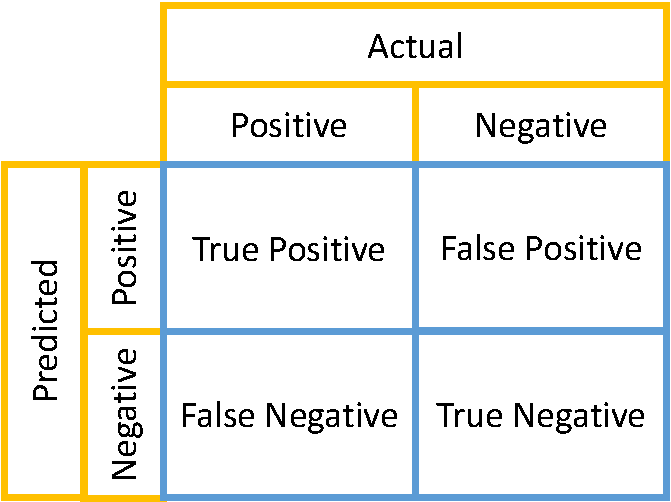
\includegraphics[width=0.55\textwidth]{images/chapter2/confusion-table.pdf}
\caption{Illustration of confusion table that summarizes prediction results of document classifiers. For simplicity, we only present classification results for binary categories. We summarize the numbers of correct and incorrect predictions with count values and broken down by each class.}
\label{chap2:fig:confusion}
\end{figure}


This section will cover five evaluation metrics of the document classification task in this thesis: accuracy, precision, recall, F1-score and area under the roc curve (AUC).
The higher those values are, the better document classifiers are, and vice versa.
We can derive scores of the five metrics by the confusion matrix table (Figure~\ref{chap2:fig:confusion}). 
The true positive (TP), false positive (FP), false negative (FN) and true negative (TN) mean that actual and predicted values are both positive, the predicted value is true while the actual value is false, the predicted value is negative while the actual value is positive, and both of predicted and actual values are negative respectively.
The confusion matrix table can tell us insights into classification performance that what types of errors are for document classifiers.


\paragraph{Accuracy} measures the correct rate of classifiers. We can calculate the accuracy score by $\frac{TP+TN}{TP+TN+FP+FN}$. Yet, the accuracy is not a good fit for imbalanced datasets. For example, if spam emails only account for 1\%, a 99\% accuracy score of a classifier is less meaningful.

\paragraph{Precision, Recall and F1-score} usually jointly measure the performance of document classification. The metrics calculate precision by $\frac{TP}{TP+FP}$, recall by $\frac{TP}{TP+FN}$ and F1-score by $2*\frac{Recall*Precision}{Recall+Precision}$.\footnote{The F1-score derives from F-$\beta$, where F-$\beta$=$\frac{(1+\beta^2)*Precision*Recall}{(\beta^2*Precision)+Recall}$. The $\beta$ is a weight factor to balance the importance of precision and recall. 
The higher $\beta$ weighs recall higher than precision, and vice versa. 
F1-score is when the F-$\beta$ treats recall and precision equally and takes $\beta$ as 1.}
Precision measures the rate of correctly predicted instances. 
Recall indicates the rate of correctly recognized positive instances. 
F1-score harmonically combines precision and recall.
Yet, class labels may have skewed distributions or different weights, particularly for multi-class classification evaluation, therefore, we can average F1-scores for individual labels differently via various modes: binary, micro, macro, weighted and samples.
The weighted F1-score leverages balance between each label by its number of true instances.
The score considers label imbalance during calculation and can obtain a score that is not related to overall precision and recall.\footnote{The other modes can be referred to \url{https://scikit-learn.org/stable/modules/generated/sklearn.metrics.f1_score.html}.}


\begin{figure}[tb!]
\centering
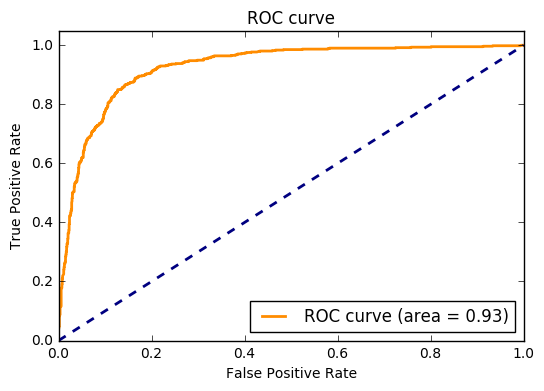
\includegraphics[width=0.85\textwidth]{images/chapter2/roc-curve.png}
\caption{Illustration of ROC curve and AUC. The AUC score can be calculated by the ROC curve, where the curves changes with classification thresholds, the X-axis indicates the FP rate and the Y-axis refers to the TP rate.}
\label{chap2:fig:roc}
\end{figure}

\paragraph{AUC} indicates how well the probabilities from the positive classes are separated from the negative classes. 
We can calculate the scores by the \texttt{roc\_auc\_score} function from Scikit-Learn~\cite{pedregosa2011scikit}.
Unlike the previous metrics depend on the probability threshold,\footnote{Usually we choose 0.5 as the threshold.} the AUC is classification-threshold-invariant.


% \section{Metadata and Language Variations}


\section{Domain Adaptation}
\label{chap2:sec:domain_adpt}
% domain adaptation definition;
% an illustration of domain adaptation in document classification;
% introduce what we will cover in this section
Domain adaptation aims to align source with target domain distributions while sharing the same labels in both source and target domains.
In this section, I will present several domain adaptation methods that will be used extensively in this thesis: feature augmentation, multitask learning and domain adversarial training.


\subsection{Feature Augmentation}
\label{chap2:subsec:feaaug}

\begin{figure}[tb!]
\centering
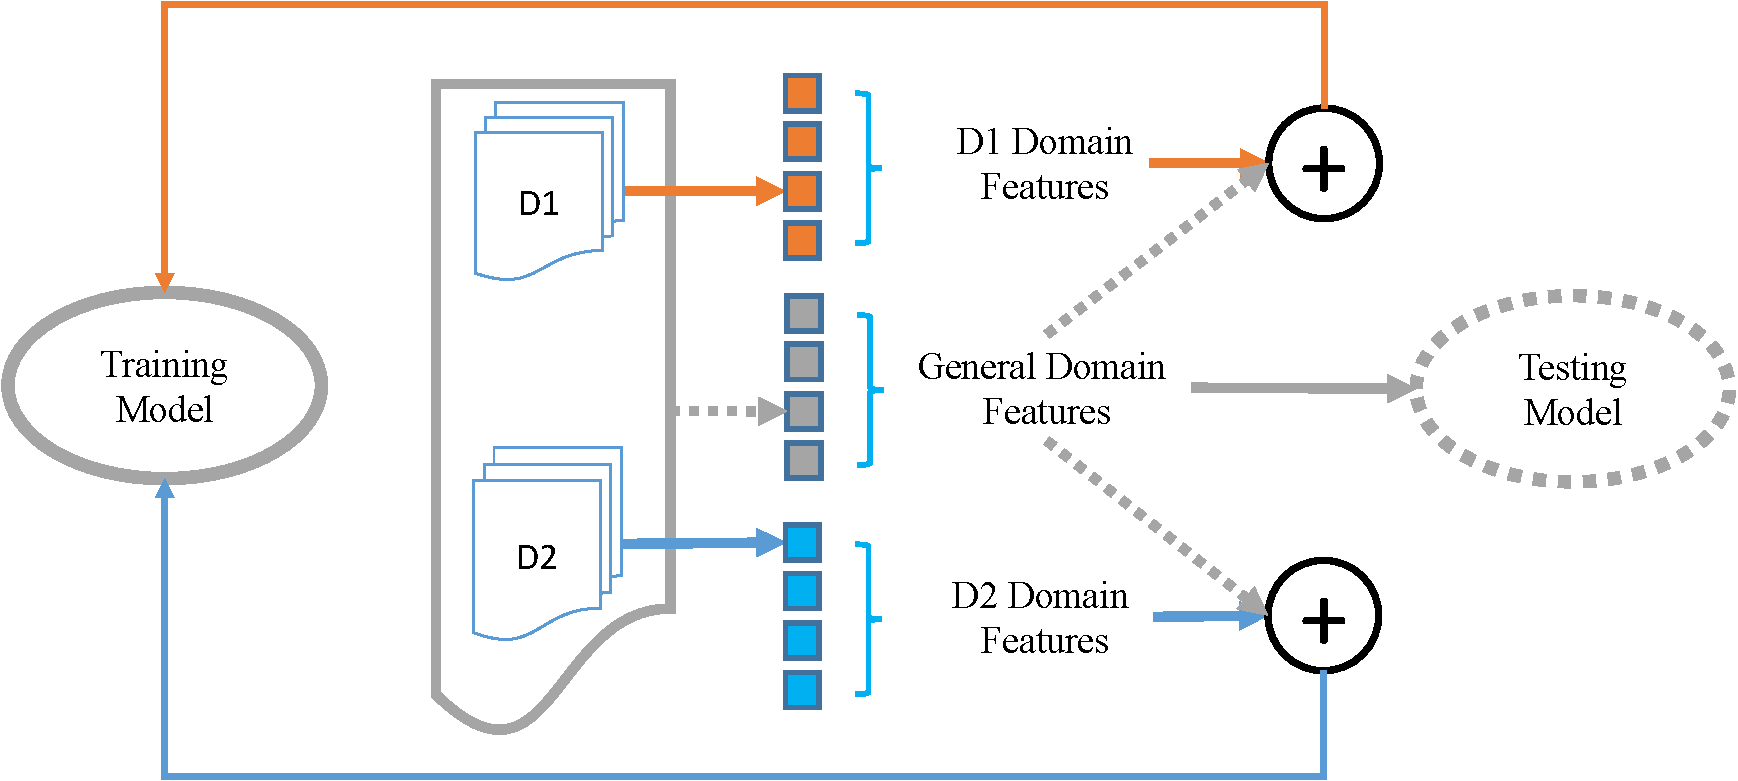
\includegraphics[width=0.90\textwidth]{images/chapter2/feature-aug.pdf}
\caption{Illustration of Frustratingly Easy Domain Adaptation~\cite{daume2007frustratingly}. We present a collection of documents that are from two different domains, ``D1'' and ``D2''. Three different colors of features means domain-specific (blue and orange) and domain-independent (gray) features. }
\label{chap2:fig:aug}
\end{figure}

Feature augmentation in domain adaptation aims to obtain domain-independent representations of documents and therefore generalize document classifiers~\cite{blitzer2006domain, daume2007frustratingly}.
We show a feature augmentation method in Figure~\ref{chap2:fig:aug}.
The methods show its effectiveness in user factor~\cite{lynn2017human} and temporality~\cite{huang2018examining} adaptation for improving and generalizing document classifiers.
The method first extracts features within each domain, domain-specific features.
Next, by treating all documents as a whole, the methods extract general features, domain-independent features.
We can format a document representation by a combination of domain-specific and independent features: $\langle X_g, X_{d1}, X_{d2} \rangle$.
A document from ``D1'' domain can be represented as $\langle X_g, X_{d1}, 0 \rangle$, and similarly, a document from ``D2'' domain can be represented as $\langle X_g, 0, X_{d2} \rangle$. 
The model will use both domain-specific and -independent features, however, the model will only use the domain-independent features.
The goal is to train a domain-independent classifier.


\subsection{Multitask Learning}

\begin{figure}[tb!]
\centering
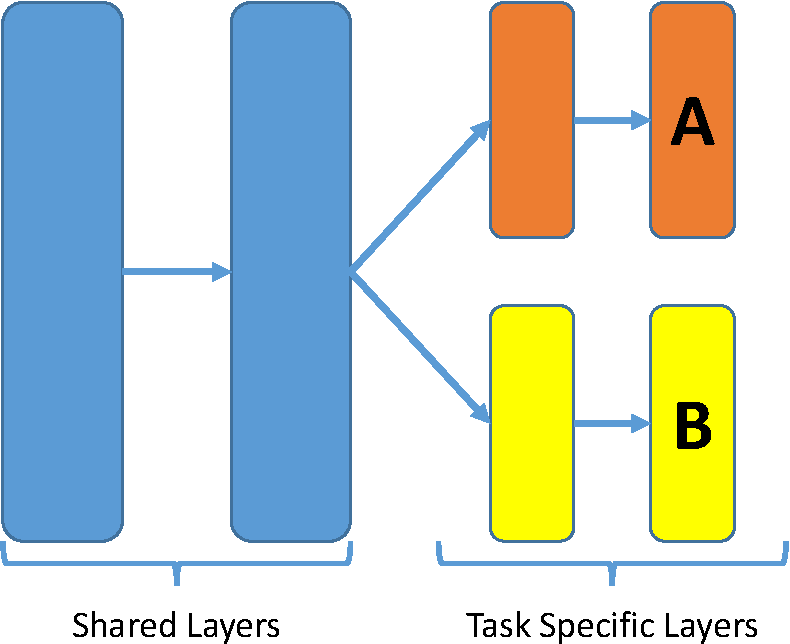
\includegraphics[width=0.65\textwidth]{images/chapter2/multitask.pdf}
\caption{Illustration of Multitask Learning with the neural model. The A and B are different prediction tasks. The two tasks shared layers in the blue color and own independent layers in the orange and yellow colors.}
\label{chap2:fig:mtl}
\end{figure}

The Figure~\ref{chap2:fig:mtl} presents a Multitask Learning (MTL) framework with a neural model architecture.
The two tasks share the first few layers while leaves independent layers for each task.
The MTL improves and generalizes each prediction task from the following three main aspects.
First, adding one more prediction task can bring more training instances for tweaking the shared layers. 
Second, the prediction tasks force the model learning task-independent representations and improve generalization by leveraging the task-specific information.
Third, the independent layers can help learn task-related patterns for document classifiers.

% http://ruder.io/multi-task/

\subsection{Domain Adversarial Training}

Domain adversarial training is a method to generalize models across domains by training document representations less sensitive and predictable towards domain categories~\cite{ganin2016domain}.
The method assumes there are two domains, source and target domains, where source domain documents have labels and target domain documents do not.
Two main loss functions are using the categorical cross entropy~\cite{goodfellow2016deep}: document class and domain predictions.
The domain class prediction is the regular prediction task, while the domain prediction is to predict if a document belongs to the source or target domain.
To generalize the document representations, the method aims to penalize the high accuracy of domain prediction.
Therefore, the method reverses the loss value of domain prediction, we can then have the following:
$$Loss = \frac{1}{n}\sum_{i=1}^n\mathcal{L}(y_i, \hat{y}_i) - \lambda(\frac{1}{n}\sum_{i=1}^n\mathcal{L}(y_s, \hat{y}_d) + \frac{1}{\hat{n}}\sum_{i=n+1}^N\mathcal{L}(y_t, \hat{y}_d))$$
, where $N$ is the total number of documents from both source and target domains, $n$ is the number of labeled documents from the source domain, $\hat{n}$ is the number of unlabeled documents from the target domain, $y$ refers to document label and $\hat{y}$ is the predicted document class, $\lambda$ indicates the weight of document prediction loss, $y_s$ and $y_t$ are the domain labels for source and target respectively, and $\hat{y}_d$ refers to the predicted domain label.
Noted that usually, the final loss values are the sum of all loss functions.
However, the domain adversarial training reverse the plus to minus in the function above, which can be viewed as an ``adversarial'' way.
And the adversarial optimization only happens during the training step.
Therefore, the method is called ``domain adversarial training''. 


\section{Temporal Variations of Language}
\label{chap2:sec:time}

Language, and therefore data derived from language, changes over time~\cite{ullmann1963modern}.
Time is implicitly embedded in the classification process: classifiers are often built to be applied to future data that doesn't yet exist, and performance on held-out data is measured to estimate performance on future data whose distribution may have changed.
This section presents an essential background of Chapter~\ref{chp:temporality}.


\subsection{Language Shifts}

\textit{Language shift} reflects the complex mutual processes between language and human society over time.
Word senses can shift over long periods \cite{hamilton2016diachronic}, and written language can change rapidly in online platforms \cite{eisenstein2014diffusion, goel2016social}.
For example, the meaning of \textit{gay} has changed from \textit{cheerful} to \textit{homosexual}~\cite{hamilton2016diachronic}, and the emoji have only become available in recent years. 
One promising solution is \textit{diachronic word embedding}, which jointly models words and temporality.


\subsection{Diachronic Word Embedding}
\label{chap2:sec:dwe}

\begin{figure}[tb!]
\centering
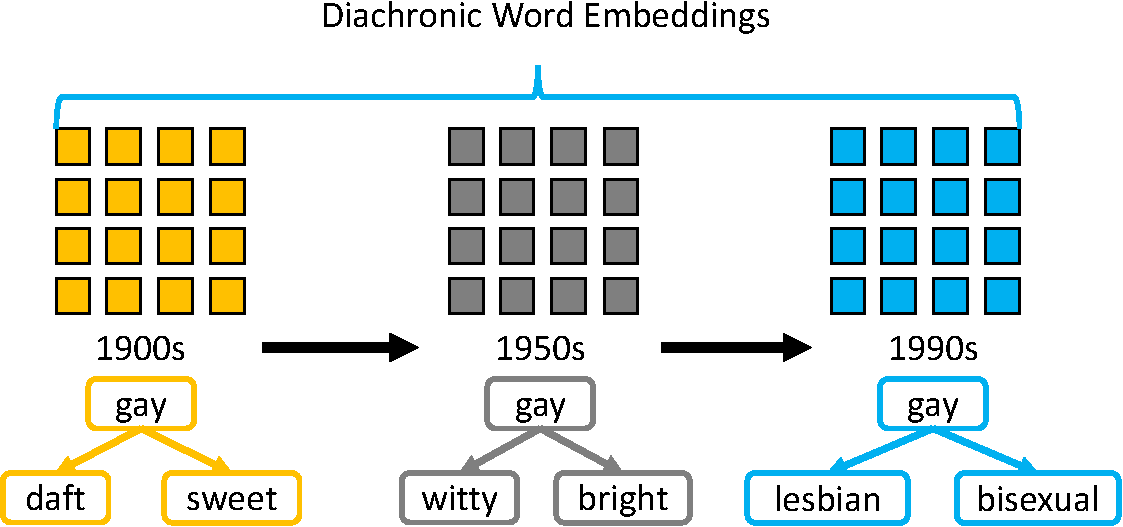
\includegraphics[width=0.85\textwidth]{images/chapter2/diachronic.pdf}
\caption{Illustration of Diachronic Word Embeddings. We introduce an existing method~\cite{kulkarni2015statistically} to train diachronic word embeddings. The time intervals use different colors to distinguish embedding models and temporal semantics. With the selected three time intervals (the 1900s, 1950s, 1990s) and diachronic word embeddings, we present a case study that how the word ``gay'' changes its close synonyms over time.}
\label{chap2:fig:diachronic}
\end{figure}

Diachronic (dynamic) word embedding (DWE) explicitly models temporality into word embedding models.
The DWE aims to capture the change of word semantic meaning over time~\cite{kutuzov2018diachronic}.
Existing research utilizes the diachronic word embedding into different tasks under the topic of semantic shifts~\cite{kutuzov2018diachronic}, such as semantic shift detection~\cite{mihalcea2012word, kim2014temporal, kulkarni2015statistically, rudolph2018dynamic, yao2018dynamic, rosenfeld2018deep}, laws of semantic change~\cite{hamilton2016diachronic, dubossarsky2017outta}, diachronic semantic relations~\cite{rosin2017learning, szymanski2017temporal}, etc.

The Figure~\ref{chap2:fig:diachronic} illustrates an example of building diachronic word embedding.
First, a corpus will be split into different time intervals, which can be seasonal~\cite{huang2018examining}, yearly~\cite{yao2018dynamic}, decade~\cite{hamilton2016diachronic}:
$$C = [d_{1, 1}, ~d_{2, 1}, ~..., ~d_{i, t}] $$
$$C_t \in C, ~~~ C_t = [d_{1, t},~ ...d_{n, t}]$$
, where $C$ is the corpus, $d$ is a document, $i$ is the index of document and $t$ is the time label, $C_t$ is a collection of documents within the $t$ time interval and $n$ is the number of documents in $C_t$.
Next, we will initialize and train a separate word embedding model for each time interval.
However, each well-trained word embedding model for each time interval are not in the same vector spaces because of the separate training steps. 
The next step is to map the embedding models into the same vector space.
The alignment function is:
$$f(W, E_{\hat{t}}) = E_t$$
, where $\hat{t}$ and $t$ are source and target time intervals respectively, $E$ is an embedding model, $f$ is the alignment function and $W$ is the function weight to learn.
This step aims to align the source ($\hat{t}$) to the target time interval ($t$).

Existing methods of aligning word embeddings focus on the following three directions: \textit{incremental training}~\cite{kim2014temporal}, \textit{matrix transformation}~\cite{kulkarni2015statistically, hamilton2016diachronic, yao2018dynamic} and \textit{temporal vectorization}~\cite{rosenfeld2018deep, huang2019neural}. 
\textit{Incremental Training} utilizes a trained embedding model to initialize the embedding weights of words in the next time interval.
\textit{Matrix Transformation} learns a transformation matrix $M \in R^{d \times d}$ by solving the following optimization:
$$argmin \sum_{i=1}^{|V|}|E_t(w_i) - E_{\hat{t}} \cdot M|^2$$
, where $|V|$ is the vocabulary size, $w_i$ is a word from the vocabulary.
\textit{Temporal vectorization} models time and word jointly. The first step is to represent time as a fixed-length vector. In contrast to the regular word representations, the new representation for each word will be:
$$\hat{E}(w_i) = f(E(w_i) \cdot W_w + T_e(t) \cdot W_t)$$
, where $\hat{E}$ is the new word embedding, $T_e$ is an embedding model of time, $w_i$ is a word, $f$ is an activation function to model word and time jointly, $W$ is the learned weight.
Training the model is similar to word embeddings in Section~\ref{chap2:subsubsec:emb}, except the input and output embeddings will represent each word vector as a combination of word and time.
We will present how our method models and vectorizes the temporal factor in Section~\ref{chap3:sec:dwe}.


\subsubsection{DWE Evaluation}

Existing DWE evaluation methods~\cite{kutuzov2018diachronic} have three general prediction tasks: cross-time analogy, time-span disambiguation and event prediction.
\textit{Cross-time analogy}~\cite{szymanski2017temporal, yao2018dynamic} is to find semantic equivalents across time intervals.
For example, the US president is close to Obama in 2015 vs. Trump in 2017 and Apple is close to fruit in 1980 vs. Microsoft in 2018.
\textit{Time span disambiguation}~\cite{mihalcea2012word, popescu2015semeval} is to determine the specific time spans that documents or words belong to. 
For example, the diachronic text evaluation~\cite{popescu2015semeval} splits documents into different time intervals and evaluates if classifiers can predict correctly the time intervals of documents.
\textit{Event prediction}~\cite{kutuzov2017tracing} is to use diachronic word embeddings to predict or trace real-world events such as gun violations and conflicts.
In this thesis, we will evaluate our proposed method by both cross-time analogy (Section~\ref{chap3:subsec:dweEval}) and document classification (Section~\ref{chap3:sec:dweExp}) tasks.


\section{User Variations of Language}
\label{chap2:sec:demographic}


Language varies across user factors including demographic factors, user profiles and user histories. 
Users can use the same words for different meanings and different words for the same meaning depending on social contexts~\cite{oba2019modeling}. 
Research has shown that user posts in social media are predictive of demographic variables such as 
gender~\cite{rao2010classifying, rao2011hierarchical, burger2011discriminating, volkova2015inferring}, age~\cite{rosenthal2011age, hovy2015tagging, johannsen2015cross, zhang2016predicting, diaz2018addressing}, race~\cite{preoctiuc2018user} and location~\cite{eisenstein2010latent, wing2011simple, wing2014hierarchical}.
For example, males and females express sentiment differently and young people use more widely emoji in their social media than elders.
Such variations can also cause biases of document classifiers towards a specific demographic group~\cite{sun2019mitigating}.
Research shows that hate speech classifiers tend to classify African American English words as a hate crime, yet such words might strongly correlate with the specific racial group and cause racial biases~\cite{davidson2019racial, sap2019risk}.
Therefore, it is necessary to model the user demographic factors into machine learning models.
In this thesis, we will extensively discuss user demographic factor adaptation (Section~\ref{chap4:sec:daa}) and user embedding (Section~\ref{chap4:sec:uemb}).
And therefore, we provide the necessary background of the two topics in the following.


\subsection{User Factor Adaptation}

\textit{User factor adaptation} integrates user demographic factors and histories into the machine learning classifiers. The demographic factors usually refer to the attributes of users, such as gender, age, geographic location, etc. Online generated user texts show demographic variations in the linguistic styles could be used for the use factor prediction~\cite{rosenthal2011age, zhang2016predicting, hovy2018improving}. The user histories are the historical contexts of users, such as previous posts or likes or retweets of the users. The user factors impact on how online users express their opinions and show promising improvements in the text classification task~\cite{volkova2013exploring, hovy2015demographic, lynn2017human, yang2017overcoming}.

Lynn et al~\cite{lynn2017human} use a feature augmentation method~\cite{daume2007frustratingly} to adapt user demographic factors into document classifiers.
The method extracts two types of features: general and user attribute dependent features. 
For example, given a document and an age attribute of the author, which is discretized into two age categories, $>24 or \leq 24$.
Then the method can represent the document with the author age 20 as:
$$<X_g, X_{a\leq24}, 0>$$
, where $X_g$ is the general feature set, and $X_a$ is the age-dependent feature set.
Alternatively, a document with the author age 30 will be:
$$<X_g, 0, X_{a>24}>$$
Finally, the method can train a document classifier with the augmented feature sets.
For the technical details, please refer to Section~\ref{chap2:subsec:feaaug}.


\subsubsection{User Embeddings}

\begin{figure}[tb!]
\centering
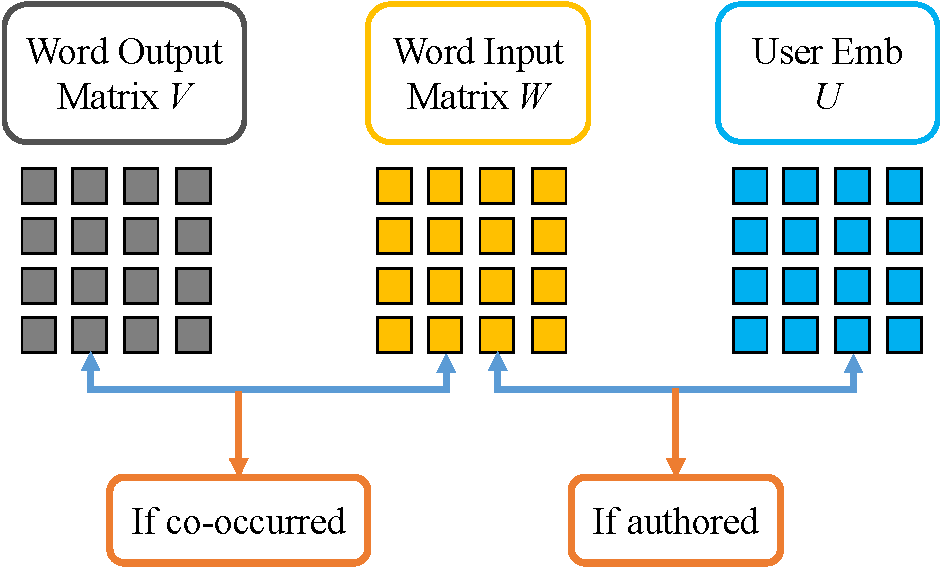
\includegraphics[width=0.85\textwidth]{images/chapter2/user-emb.pdf}
\caption{Illustration of Training User Embeddings via Skip-gram~\cite{amir2017quantifying}. $V$ is the randomly initialized output matrix of word representations, $W$ is the randomly initialized input matrix of word representations, and $U$ is the randomly initialized matrix of user embedding.}
\label{chap2:fig:user}
\end{figure}

User embedding is to model latent human traits and behaviors and map the features into a fixed low dimensional representations~\cite{pan2019social}. 
Common features include user-generated reviews, user profiles and networking connections. 
Yet, not every dataset has networking connections. 
And in this thesis, we only consider user-generated text documents and profile information.
To generate the user features, general approaches encode users through n-gram features~\cite{benton2016learning}, LDA~\cite{zhang2015using, ding2017multi}, Word2vec~\cite{amir2016modelling, benton2016learning, amir2017quantifying, wu2018starspace}, Doc2vec~\cite{ding2017multi, ding2018predicting}, etc.
% The generated user features are usually multiple views of user behaviors. 
% To map the multi-view features into a fixed representation, researchers have deployed methods including concatenation~\cite{pennacchiotti2011machine}, average~\cite{ding2017multi}, Generalized Canonical Correlation Analysis (GCCA)~\cite{benton2016learning}.
Using Skip-gram to jointly train word and user embeddings is a common way to obtain fixed representations of users~\cite{amir2017quantifying, wu2018starspace}, as shown in Figure~\ref{chap2:fig:user}.
The model jointly trains two prediction tasks at the same time: predicting if the input words are mutual contexts or not and if users used the input words.
The joint tasks aim to learn user representations $U$ from the language usage of users $W$.


\section{Demographic Bias in NLP}

Machine learning models learn \textit{demographic bias} from human language.
Fairness is especially critical to public health research, which analyzes across demographic groups. 
Language variations across demographic groups have raised people's concerns that the demographic variations can prohibit building \textit{fair} document classifiers~\cite{sun2019mitigating, bender2018data}. 
For example, unintended bias~\cite{dixon2018measuring}, which highly correlates with demographic factors, will make classifiers discriminatory in that classifiers will perform better for some demographic groups than others. 
Word embeddings, which are widely used in classification tasks, are prone to learning demographic stereotypes.
For example, a study~\cite{bolukbasi2016man} found that the word ``programmer'' is more similar to ``man'' than ``woman'', while ``receptionist'' is more similar to ``woman''.


\subsection{Debiasing Methods}

To reduce learning biases for document classifiers, existing research falls into three main directions: debiased word embeddings~\cite{zhao2017men}, data augmentation~\cite{dixon2018measuring, zhao2019gender} and model fine tuning~\cite{park2018reducing}.
\textit{Debiased Word Embeddings} is to adjust embeddings the distance balance between demographic related pronouns and concepts, such as he/she with an engineer.
\textit{Data Augmentation} is to neutralize document classifiers by changing training corpora: word blindness or replacement. 
The core idea is to either remove demographic pronouns or replace sensitive words with neutralized words.
For example, we can remove gender related words including  ``he/she'' or ``male/female'' from the corpora to prevent classifiers from judging the documents by the sensitive words.
\textit{Model Fine Tuning} focuses on adjusting trained models on the target dataset. The method first trains a document classifier on a larger and less-biased corpus, which is similar to the target corpus. 
Next, the method adjusts the hyperparameters of the trained model on the target corpus.


\subsection{Fairness Evaluation}

Fairness evaluation of document classifiers focuses on examining whether document classifiers perform differently across demographic groups, such as male and female.
In this thesis, we particularly focus on group fairness measurement~\cite{hardt2016equality}. 
The motivation is to evaluate equal opportunity between demographic groups.
Existing research~\cite{dixon2018measuring, garg2019counterfactual, park2018reducing} evaluate the author-level fairness of document classifiers by: AUC and \textit{equality differences} (ED) of true positive/negative and false positive/negative rates.

The ED sums the differences between the rates within specific user groups and the overall rates:
$$ED = \sum_{g \in G}|Rate - Rate_g|$$
, where the G is a set of demographic groups, g is one demographic group in the set, $Rate$ indicates one of true positive/negative and false positive/negative rates across the whole group, and $Rate_g$ is one type of rates such as female's false positive rate.

\chapter{Temporality Adaptation}
\label{chp:temporality}

\section{Introduction}
Language changes and varies over time,
which can cause a degradation of performance in
natural language processing models over time.
For example, document classifiers are typically trained on historical data and tested on future data, where the performance tends to be worse.
Recent research has shown that document classifiers can become more stable over time when trained in ways that specifically account for temporal variations~\cite{he2018time}.
We refer to this task of accounting for such variations during training as {\em temporality adaptation}.
This chapter is based on materials from~\cite{huang2018examining, huang2019neural}.\footnote{The improved dataset along with the code are available on: \\\url{https://github.com/xiaoleihuang/Neural_Temporality_Adaptation}, \\\url{https://github.com/xiaoleihuang/Domain_Adaptation_ACL2018}.}

This chapter organizes into three main parts.
It starts with introducing six English and Chinese datasets from both social media and newspaper sources, spanning varying lengths in time (from several decades to only a few years) in Section~\ref{chap3:sec:data}. 
Each dataset is split into a small set of time intervals, and we define each time interval as a domain. 
The section conducts analysis on the language shifts from three aspects: word, topic, context levels. 
Moreover, the section investigates how the language shifts impact on the performance of document classifiers.

The Section~\ref{chap3:sec:fa} and Section~\ref{chap3:sec:dwe} propose two temporality adaptation methods via feature augmentation and diachronic word embedding (DWE).

The first one explores \textit{feature augmentation} to integrate the temporal factor into document classifiers.
The approach considers both long-term variations in text over time and seasonal variations which change throughout a year but repeat across years.
The proposed method extends the existing domain adaptation method~\cite{daume2007frustratingly} and augment document representations by adding time domain dependent feature sets.
While the training process uses both domain dependent and independent features, the testing phase only uses domain independent feature sets.
The goal is to learn and train domain-independent document features and classifiers.
The experiments show that out-of-the-box domain adaptation techniques can make $n$-gram classifiers more robust to temporal shifts.

The second approach explores temporality adaptation from the {\em diachronic} word embeddings~\cite{kutuzov2018diachronic} perspective and further integrates the dynamic word embeddings into a time-driven neural classifier.
The proposed diachronic word embedding learns dynamic word representations from the subword level, where the embedding model represents a word by its subword components. 
Evaluation on a standard new corpus proves the effectiveness of our proposed model. 
To adapt temporality into document classifiers, we propose a time-driven neural classifier that encode documents in the view of diachronic word embeddings.
Experiments on several time-varying classification datasets demonstrate that diachronic word embedding can generally improve model performance and the proposed time-driven classifier consistently outperforms strong baselines. 

% Main contributions
Detailed contributions of this chapter as follows:

\begin{enumerate}
    \item We conduct detailed analysis to understand why and how the language shifts as they relate to important features for document classification. We examine the language shifts from word, context, topic and semantic aspects.
    \item We applied a simple domain adaptation method via feature augmentation on both yearly and monthly varying corpora.
    \item We proposed a subword-level method for constructing diachronic words embeddings, which we show to be competitive with prior approaches. 
    \item We expand this line of work by additionally considering neural adaptation models, which can also take advantage of diachronic word embeddings. We show that neural classifiers which use these embeddings can perform better on future data. 
\end{enumerate}


\section{Related Work}
\label{chap3:sec:survey}

Language evolves over time with the increasing available online data. 
With recent progress in deep neural representation learning, emerging work have been probing into the language shifting issue from the view of diachronic or dynamic word embedding perspective~\cite{tang2018state, kutuzov2018diachronic}.
These studies have shown that shifts in the corpora across time cause changes in word contexts and consequently, changes in the learned representations. 
Existing research~\cite{kim2014temporal, hamilton2016diachronic, yao2018dynamic, kutuzov2018diachronic} learns diachronic word embeddings from the word level, which creates a word representation in each time span separately for a same word. However, such a method may have three main issues: first, creating such duplicated word embedding models consumes a much higher complexity of time, memory and space; second, the colloquium and misspelling words in social media data may degrade effectiveness of word-level embedding models; third, the fixed size of the model vocabulary across time spans may not be robust enough for future incoming new words.
This chapter (Section~\ref{chap3:sec:dwe}) proposes a diachronic word embedding model based on the subword level~\cite{huang2019neural}, which compose a word representation by subword components. The subword model can solve the three main issues.
To encode the temporal factor into embedding models, existing methods develop three main directions, incremental training~\cite{kim2014temporal}, linear alignment~\cite{kulkarni2015statistically, hamilton2016diachronic} and vector representation~\cite{rosenfeld2018deep, huang2019neural}.
In this chapter, we treat the time as a subword component and vectorize the component into a fixed length of vector representation.
From the application perspective, while other research has applied diachronic word embeddings to semantic change detection and validation~\cite{mihalcea2012word, kim2014temporal, kulkarni2015statistically, hamilton2016diachronic, dubossarsky2017outta, yao2018dynamic, rudolph2018dynamic, rosenfeld2018deep, hu2019diachronic}, semantic relation analysis~\cite{liao2016analysing, szymanski2017temporal, rosin2017learning} and recent work in the named entity recognition~\cite{rijhwani2020temporally}, these types of embeddings have not been studied particularly for the document classification task.

Time is implicitly embedded in the document classification process: 
classifiers are often built to be applied to future data that doesn't yet exist,
and performance on held-out data is measured to estimate performance on future data whose distribution may have changed.
Methods exist to adjust for changes in the data distribution ({\em covariate shift}) \cite{shimodaira2000improving, bickel2009discriminative},
but time is not typically incorporated into such methods explicitly.
One line of work that explicitly studies the relationship between time and the distribution of data is work on classifying the time period in which a document was written ({\em document dating}) \cite{Kanhabua08, chambers2012labeling, Kotsakos:2014:BAD:2600428.2609495}.
However, this task is directed differently from our work: predicting timestamps given documents, rather than predicting information about documents given timestamps.
Recent work~\cite{desai2019adaptive} used the student and teacher framework to constrained feature variations across domains for classifying whether documents are political, however, the main experimental settings in the work are different from ours, which the training set does not have time spans and do not explicitly augment document representations on the time. The work mainly focused on different source domains (New York Times vs. others) instead of the temporal domain which is our main focus in this thesis.


\section{Time-Varying Corpora}
\label{chap3:sec:data}

The way people use words to express opinions has been constantly changing over time~\cite{mihalcea2012word, kulkarni2015statistically, hamilton2016diachronic}. In this section, we introduce our corpora for this chapter and conduct initial analyses on how word usage shifts over time in news articles and social media data in both English and Chinese with respect to the task of classification. We explore the language shift issue from two perspectives: word usage variation, context shift and topic change. We then examine how the language variations impact on the document classification task.

\subsection{Data}
We retrieved available data sources from previous publications~\cite{zhang2014explicit, he2016ups, huang2018examining}. Specifically, we use four different sources in in English---Amazon (music reviews), Yelp (restaurant and hotel reviews), Twitter (vaccine tweets), economic newspaper articles~\cite{figure_eight_2015} and political sentences from the American party platforms of Republicans and Democrats from 1948 to 2016, available every four years \footnote{\url{https://www.comparativeagendas.net/datasets_codebooks}} and one source in Chinese, Dianping~\cite{meituan-dianping_2019}.
The \textit{Twitter} data is annotated with binary labels indicating whether the user received an influenza vaccination (i.e., a flu shot)~\cite{huang2017examining}.
The \textit{Economy} data is annotated with binary labels indicating if each article relates to the US economy. 
For the review data (\textit{Amazon, Dianping} and \textit{Yelp}), we encode the review scores according to the experimental settings in Section~\ref{chap3:sec:fa} and Section~\ref{chap3:sec:dwe}. We discarded reviews that had fewer than 10 tokens or a helpfulness/usefulness score of zero. 

Our experiments require documents to be grouped into time intervals.Documents that fall outside of these time intervals were removed. Following \cite{huang2018examining}, we group the corpora into the following two types of temporal intervals:

\begin{itemize}[leftmargin=*,itemsep=0ex]
\item {\bf Seasonal:} Time intervals within a year (e.g., January through March) that may be repeated across years.
\item {\bf Non-seasonal:} Non-repeating time intervals spanning one or more years (e.g., 1997-1999).
\end{itemize}

Table~\ref{chap3:tab:data} shows the intervals for each corpus. 
We encode each temporal domain into the discrete time labels, $1, 2, ...T$. One corpus then can be represented as $C = [C_1, C_2, ...C_T]$, where each $C_t$ for $t\in T$ is one temporal slice of the document collection.

% For the review data (\textit{Amazon, Dianping} and \textit{Yelp}), we encode review scores into three discrete categories: score $>$3 as positive, $=$3 as neutral, and $<$3 as negative.
% The reviews with neutral scores were removed.

\begin{table*}
\centering
\resizebox{\textwidth}{!}{
\begin{tabular}{|l|l|l|l|}
\hline
\bf Dataset & \bf Time intervals (non-seasonal) & \bf Time intervals (seasonal) & \bf Size \\
\hline
Amazon & 1997-99, 2000-02, 2003-05, 2006-08, 2009-11, 2012-14 & Jan-Mar, Apr-Jun, Jul-Sep, Oct-Dec & 653K \\
Dianping & 2009, 2010, 2011, 2012 & n/a & 671K  \\
Economy & 1950-70, 1971-85, 1986-2000, 2001-14 & Jan-Mar, Apr-Jun, Jul-Sep, Oct-Dec & 6.29K  \\
Politics & 1948-56, 1960-68, 1972-80, 1984-92, 1996-2004, 2008-16 & n/a & 35.8K  \\
Twitter & 2013, 2014, 2015, 2016 & Jan-Mar, Apr-Jun, Jul-Sep, Oct-Dec & 9.83K  \\
Yelp-hotel & 2005-08, 2009-11, 2012-14, 2015-17 & Jan-Mar, Apr-Jun, Jul-Sep, Oct-Dec & 78.6K \\
Yelp-rest & 2005-08, 2009-11, 2012-14, 2015-17 & Jan-Mar, Apr-Jun, Jul-Sep, Oct-Dec & 1.16M  \\
\hline
\end{tabular}
}
\caption{Descriptions of corpora spanning multiple time intervals. Size is the number of documents. We use Yelp-hotel and -rest to denote the review data for hotel and restaurant categories. The $n/a$ denotes no time spans for the corresponding dataset.}
\label{chap3:tab:data}
\end{table*}


\subsection{Analysis 1: Word Usage Shift}
\label{chap3:subsec:wusage}

\begin{figure}[tb!]
\centering
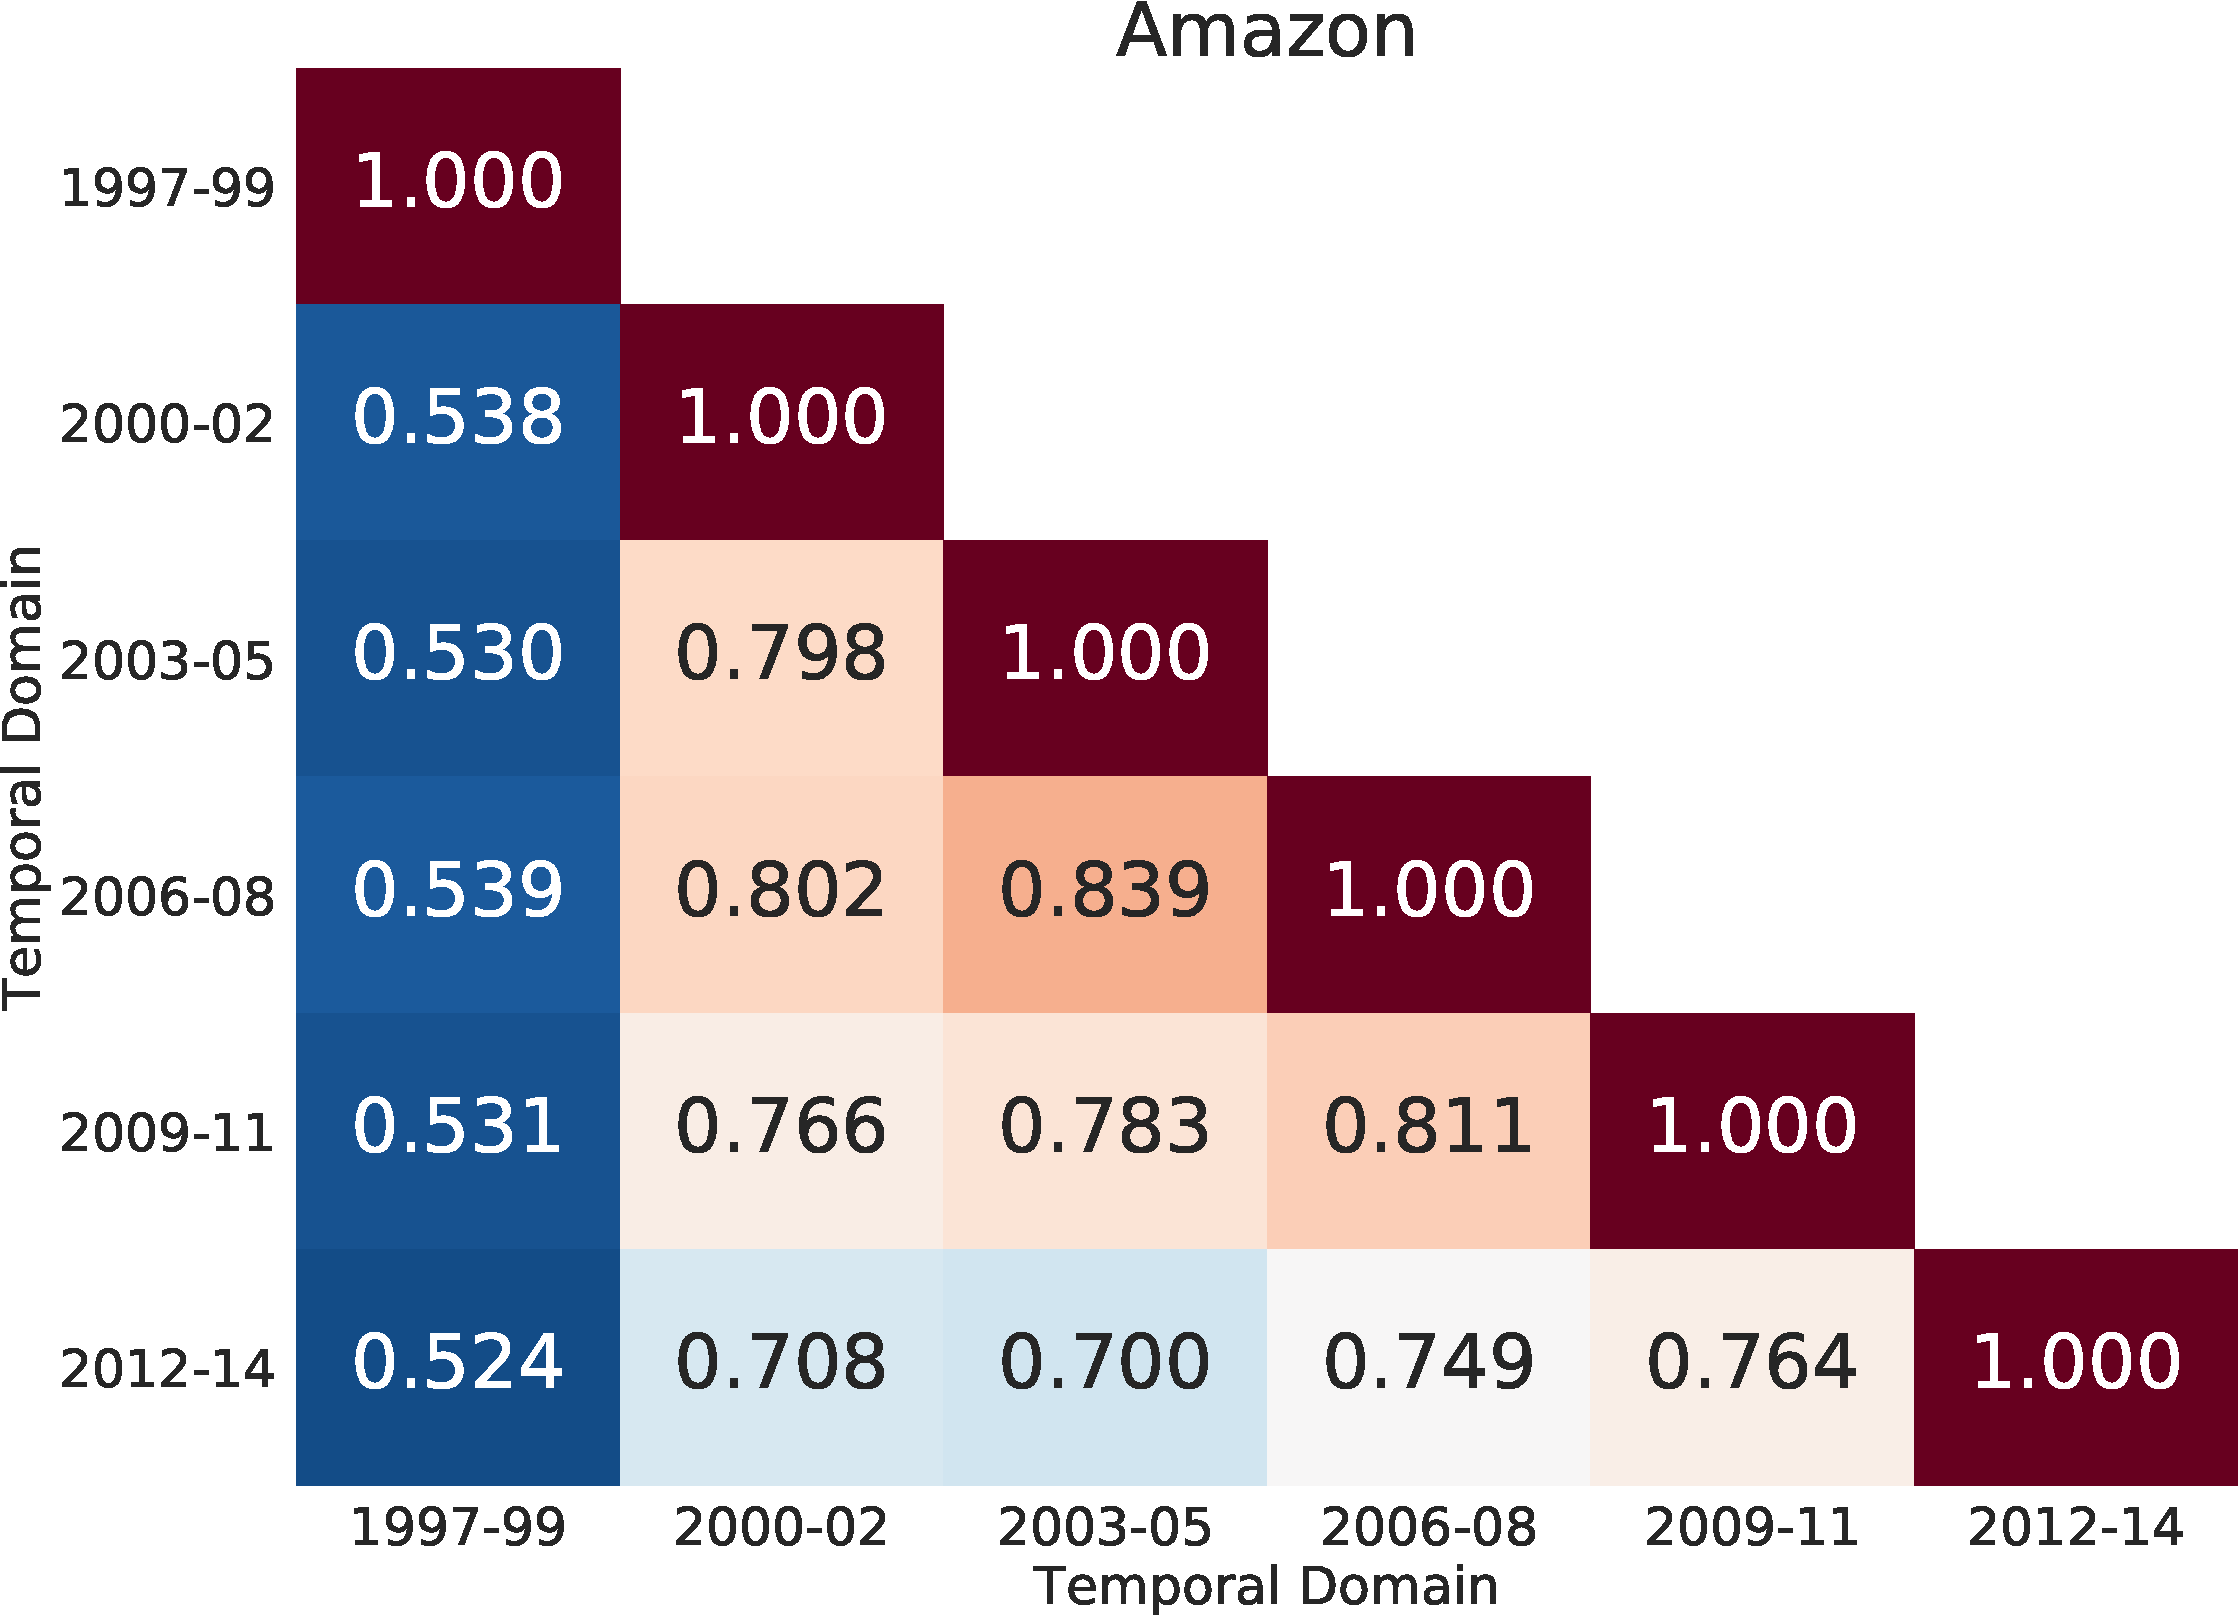
\includegraphics[width=0.31\textwidth]{images/chapter3/lang_use/amazon.pdf}
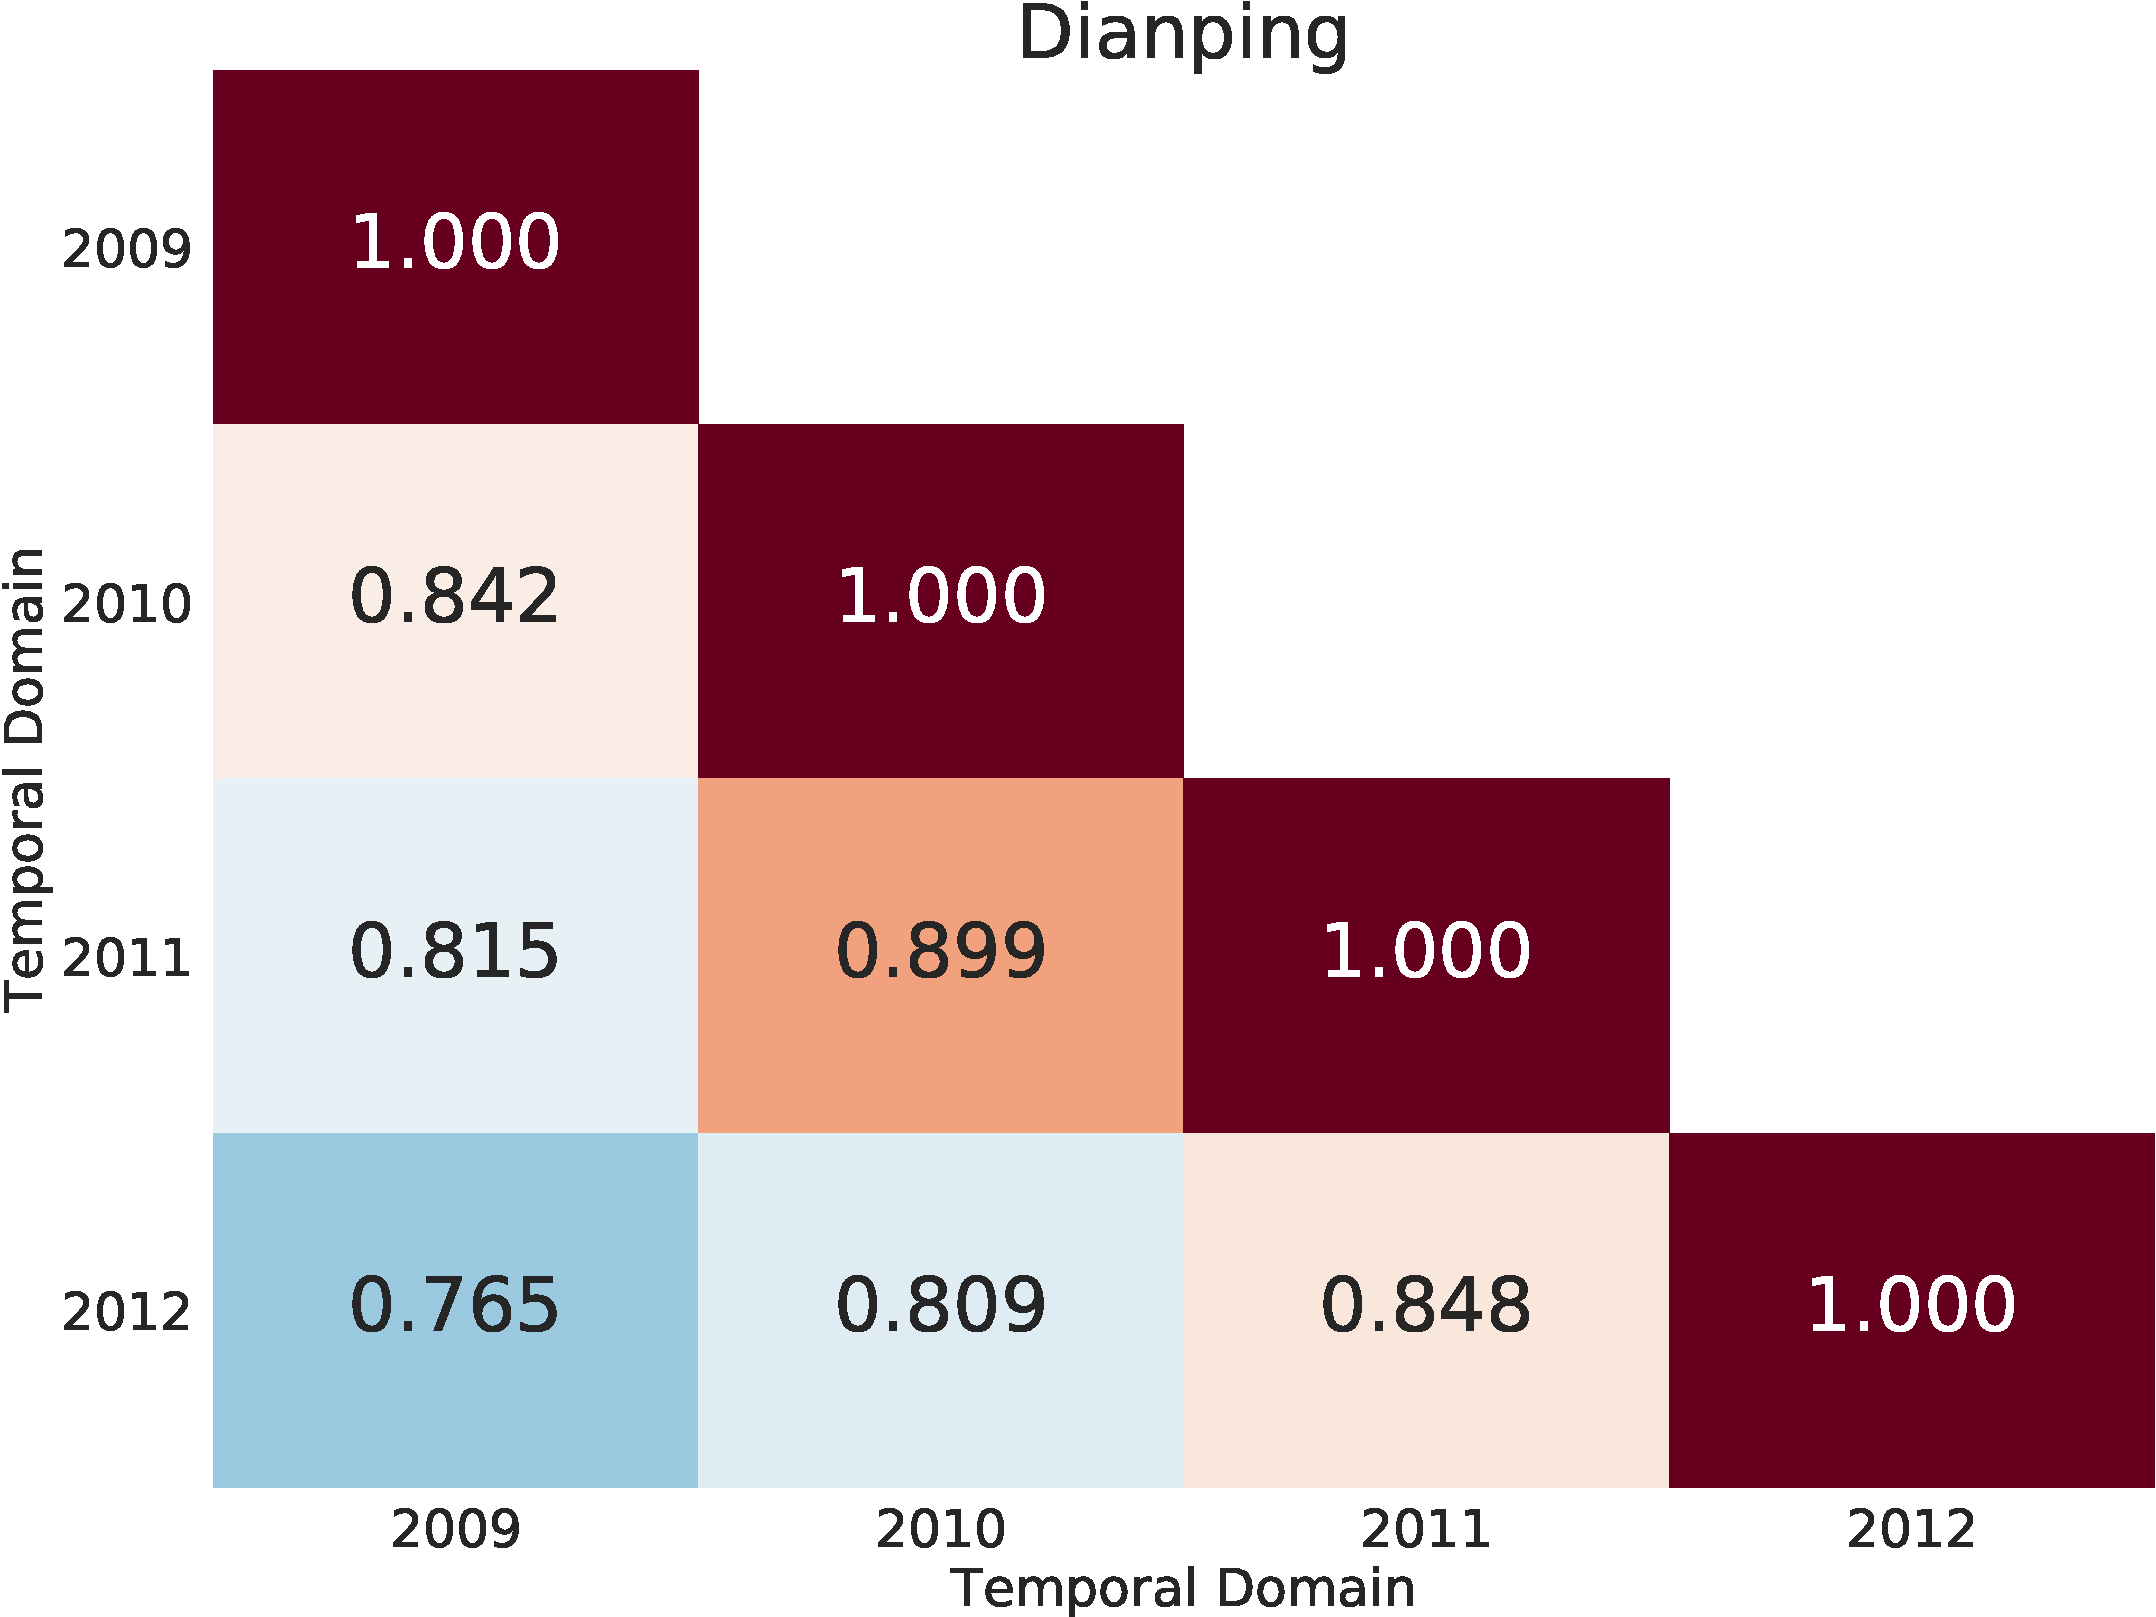
\includegraphics[width=0.31\textwidth]{images/chapter3/lang_use/dianping.pdf}
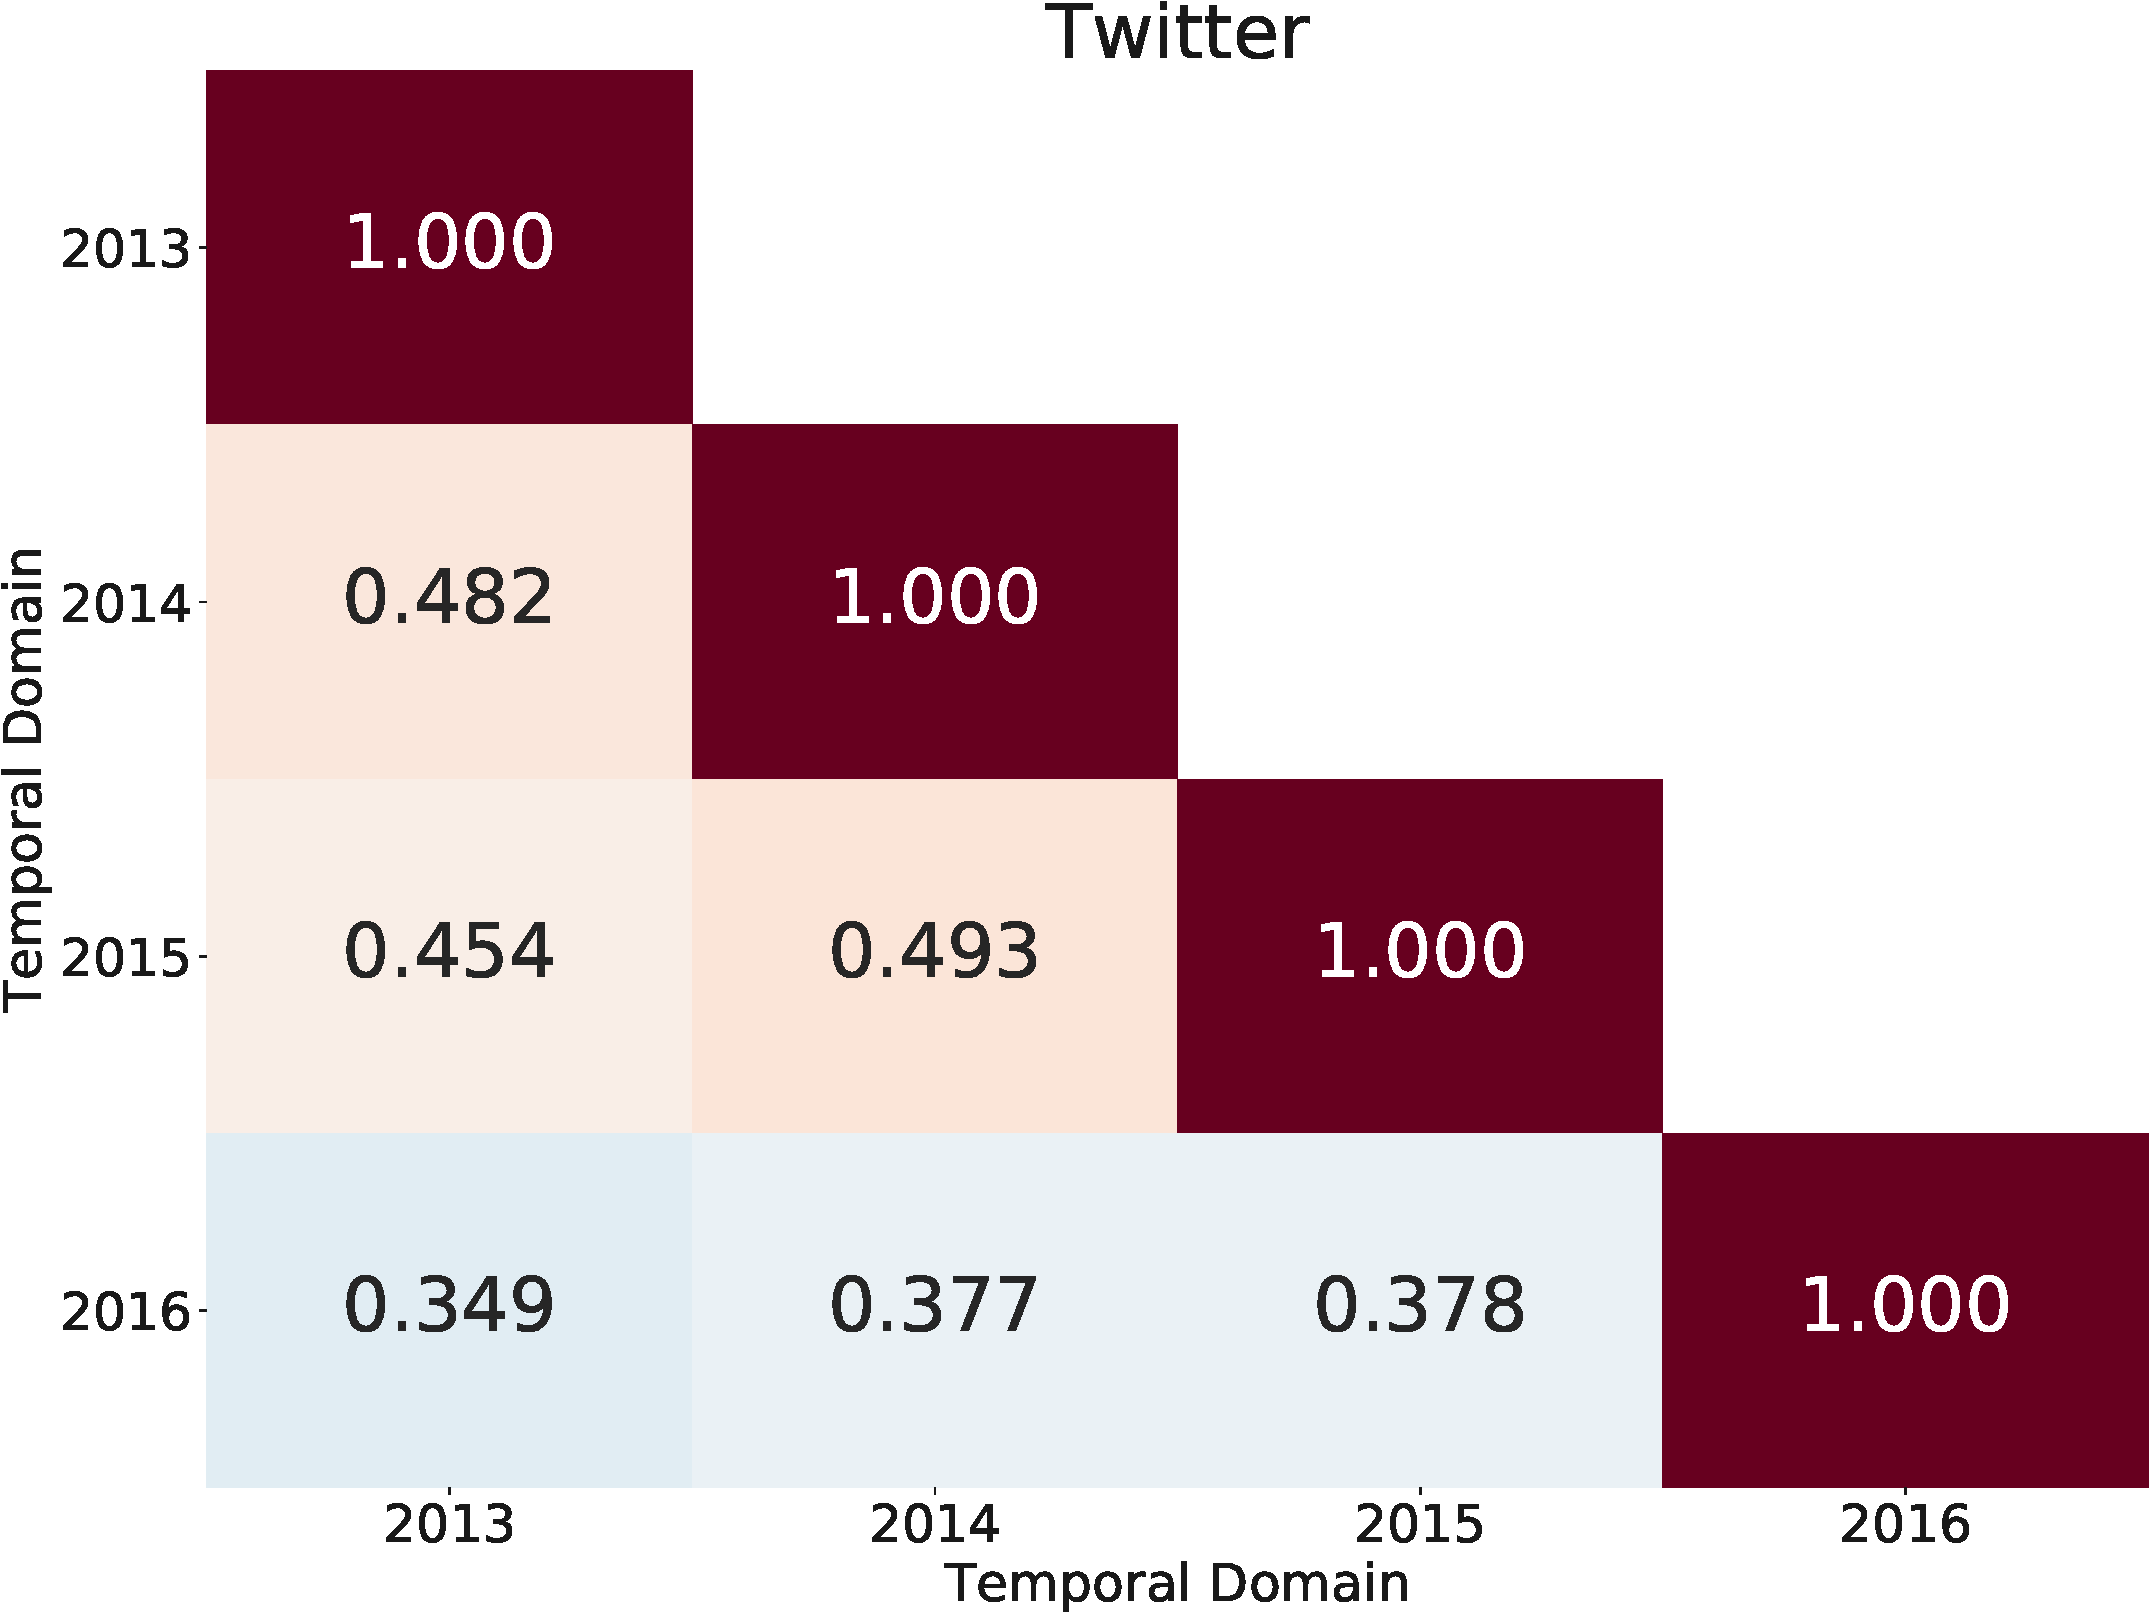
\includegraphics[width=0.31\textwidth]{images/chapter3/lang_use/vaccine.pdf}
\newline
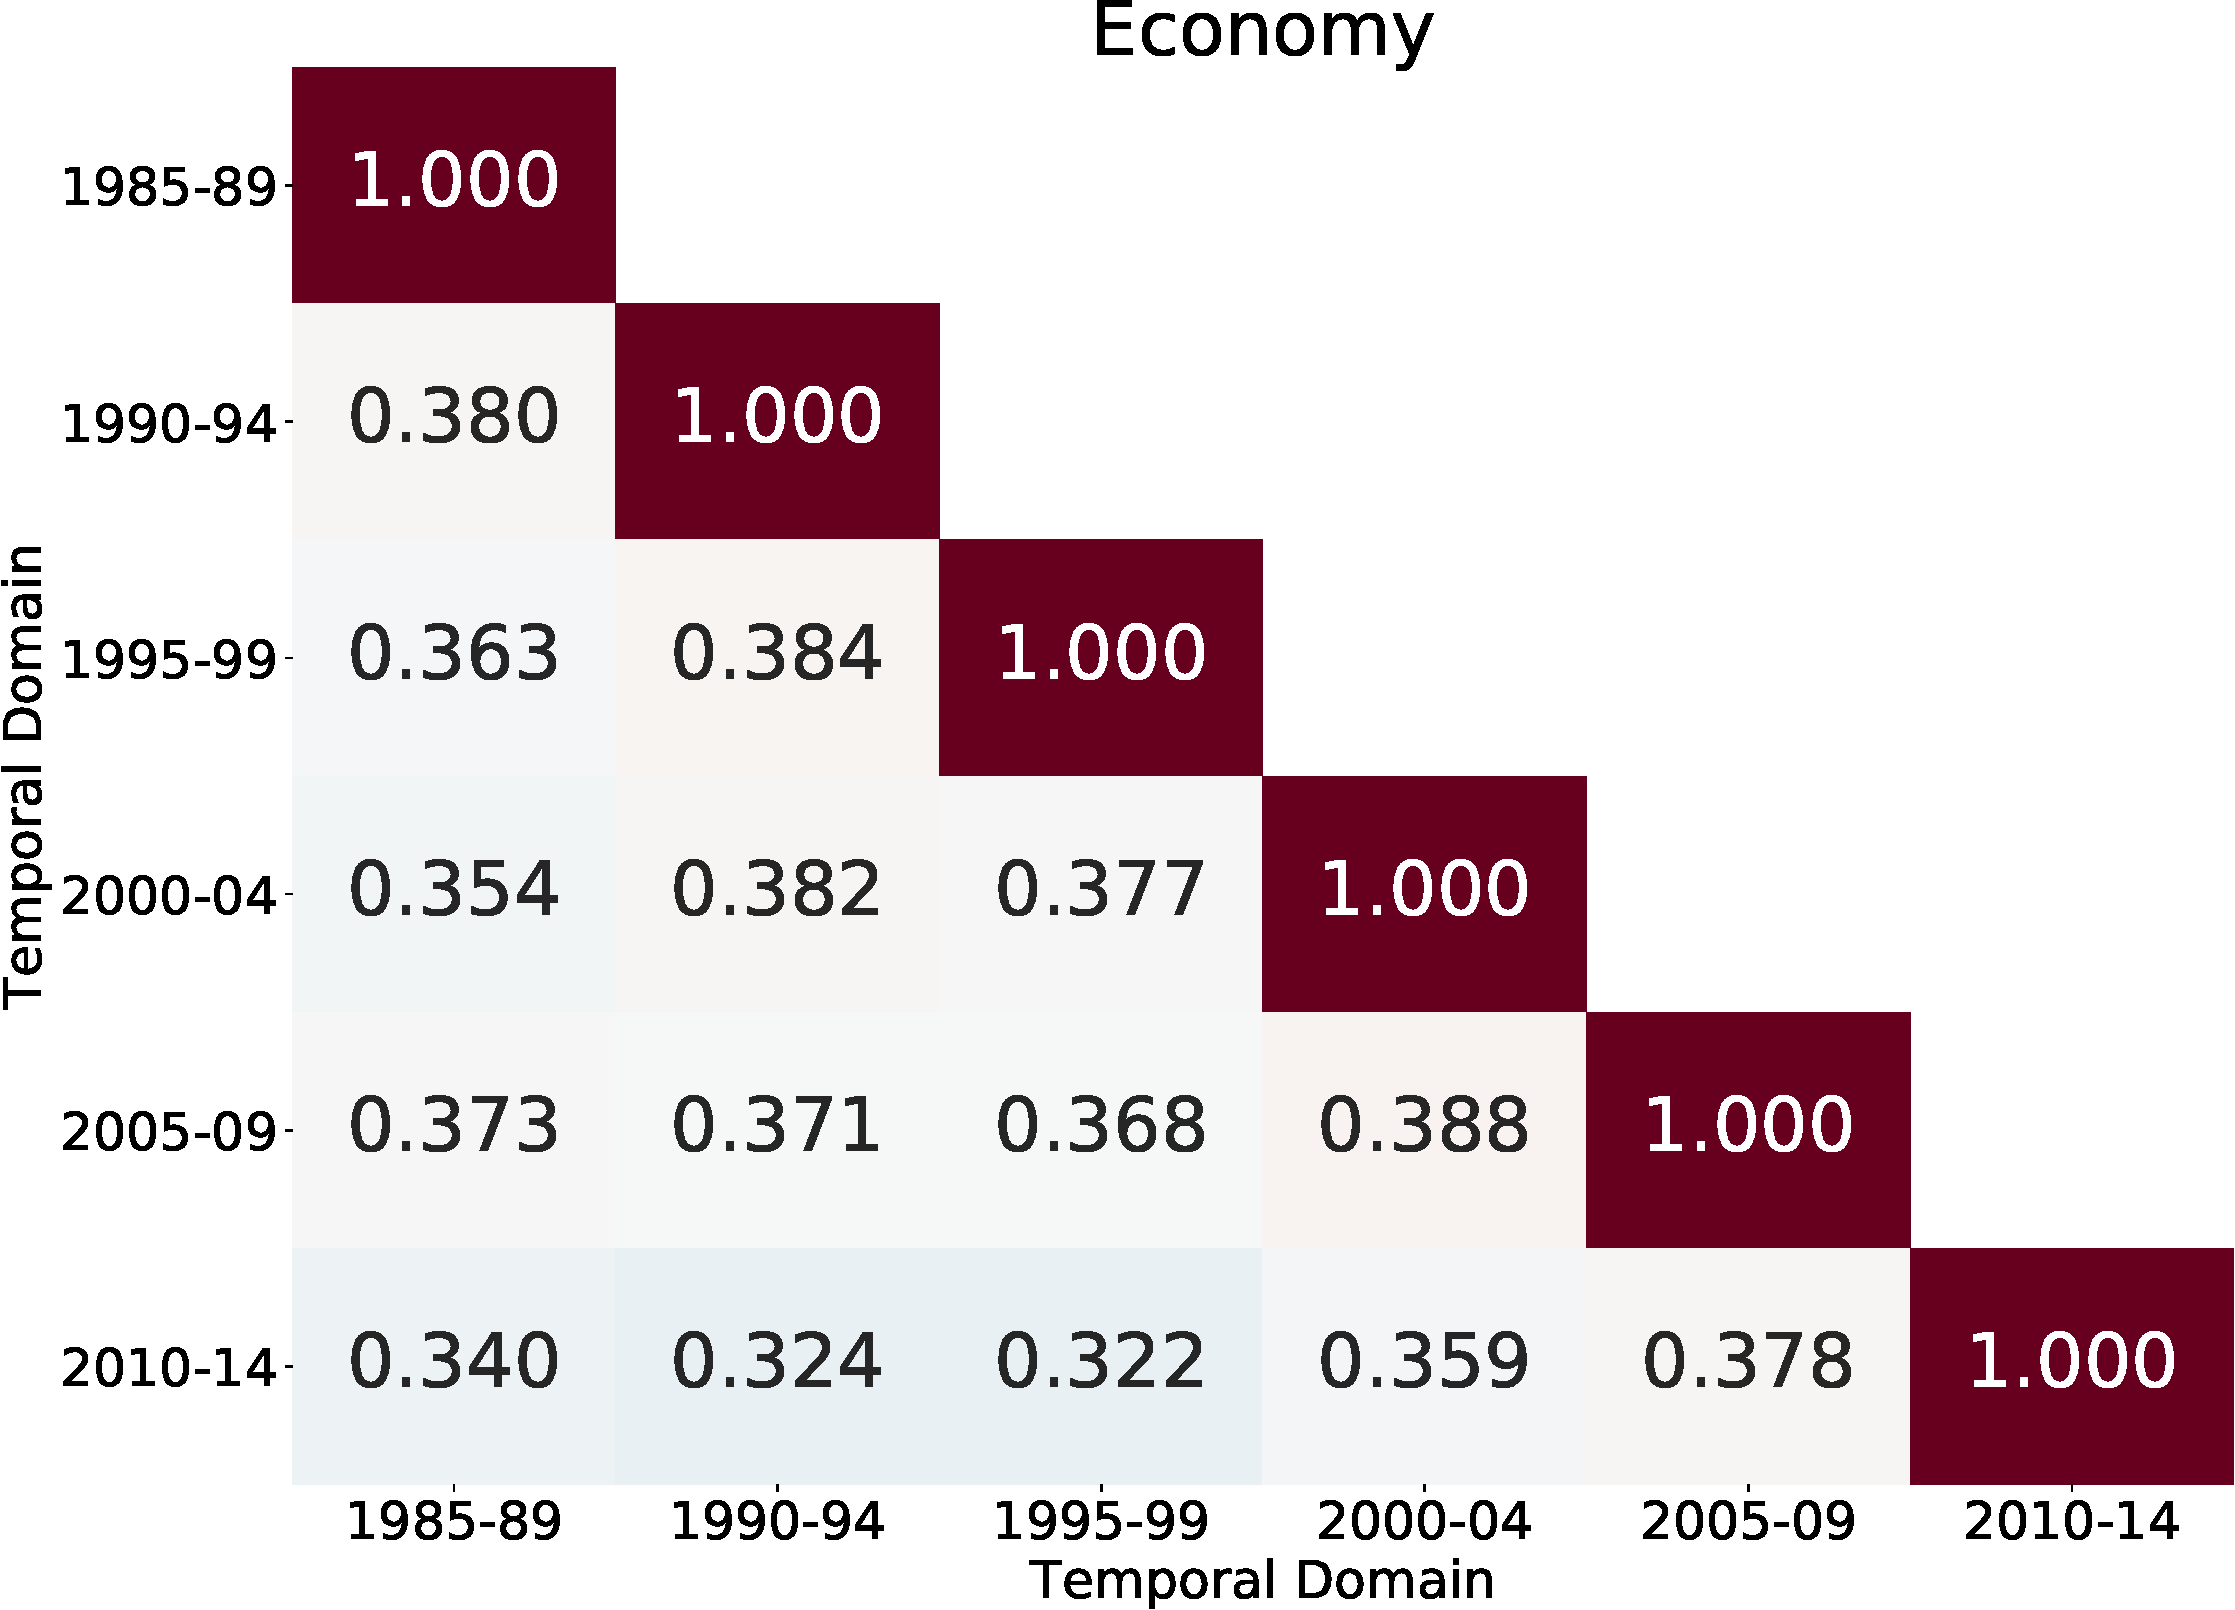
\includegraphics[width=0.31\textwidth]{images/chapter3/lang_use/economy.pdf}
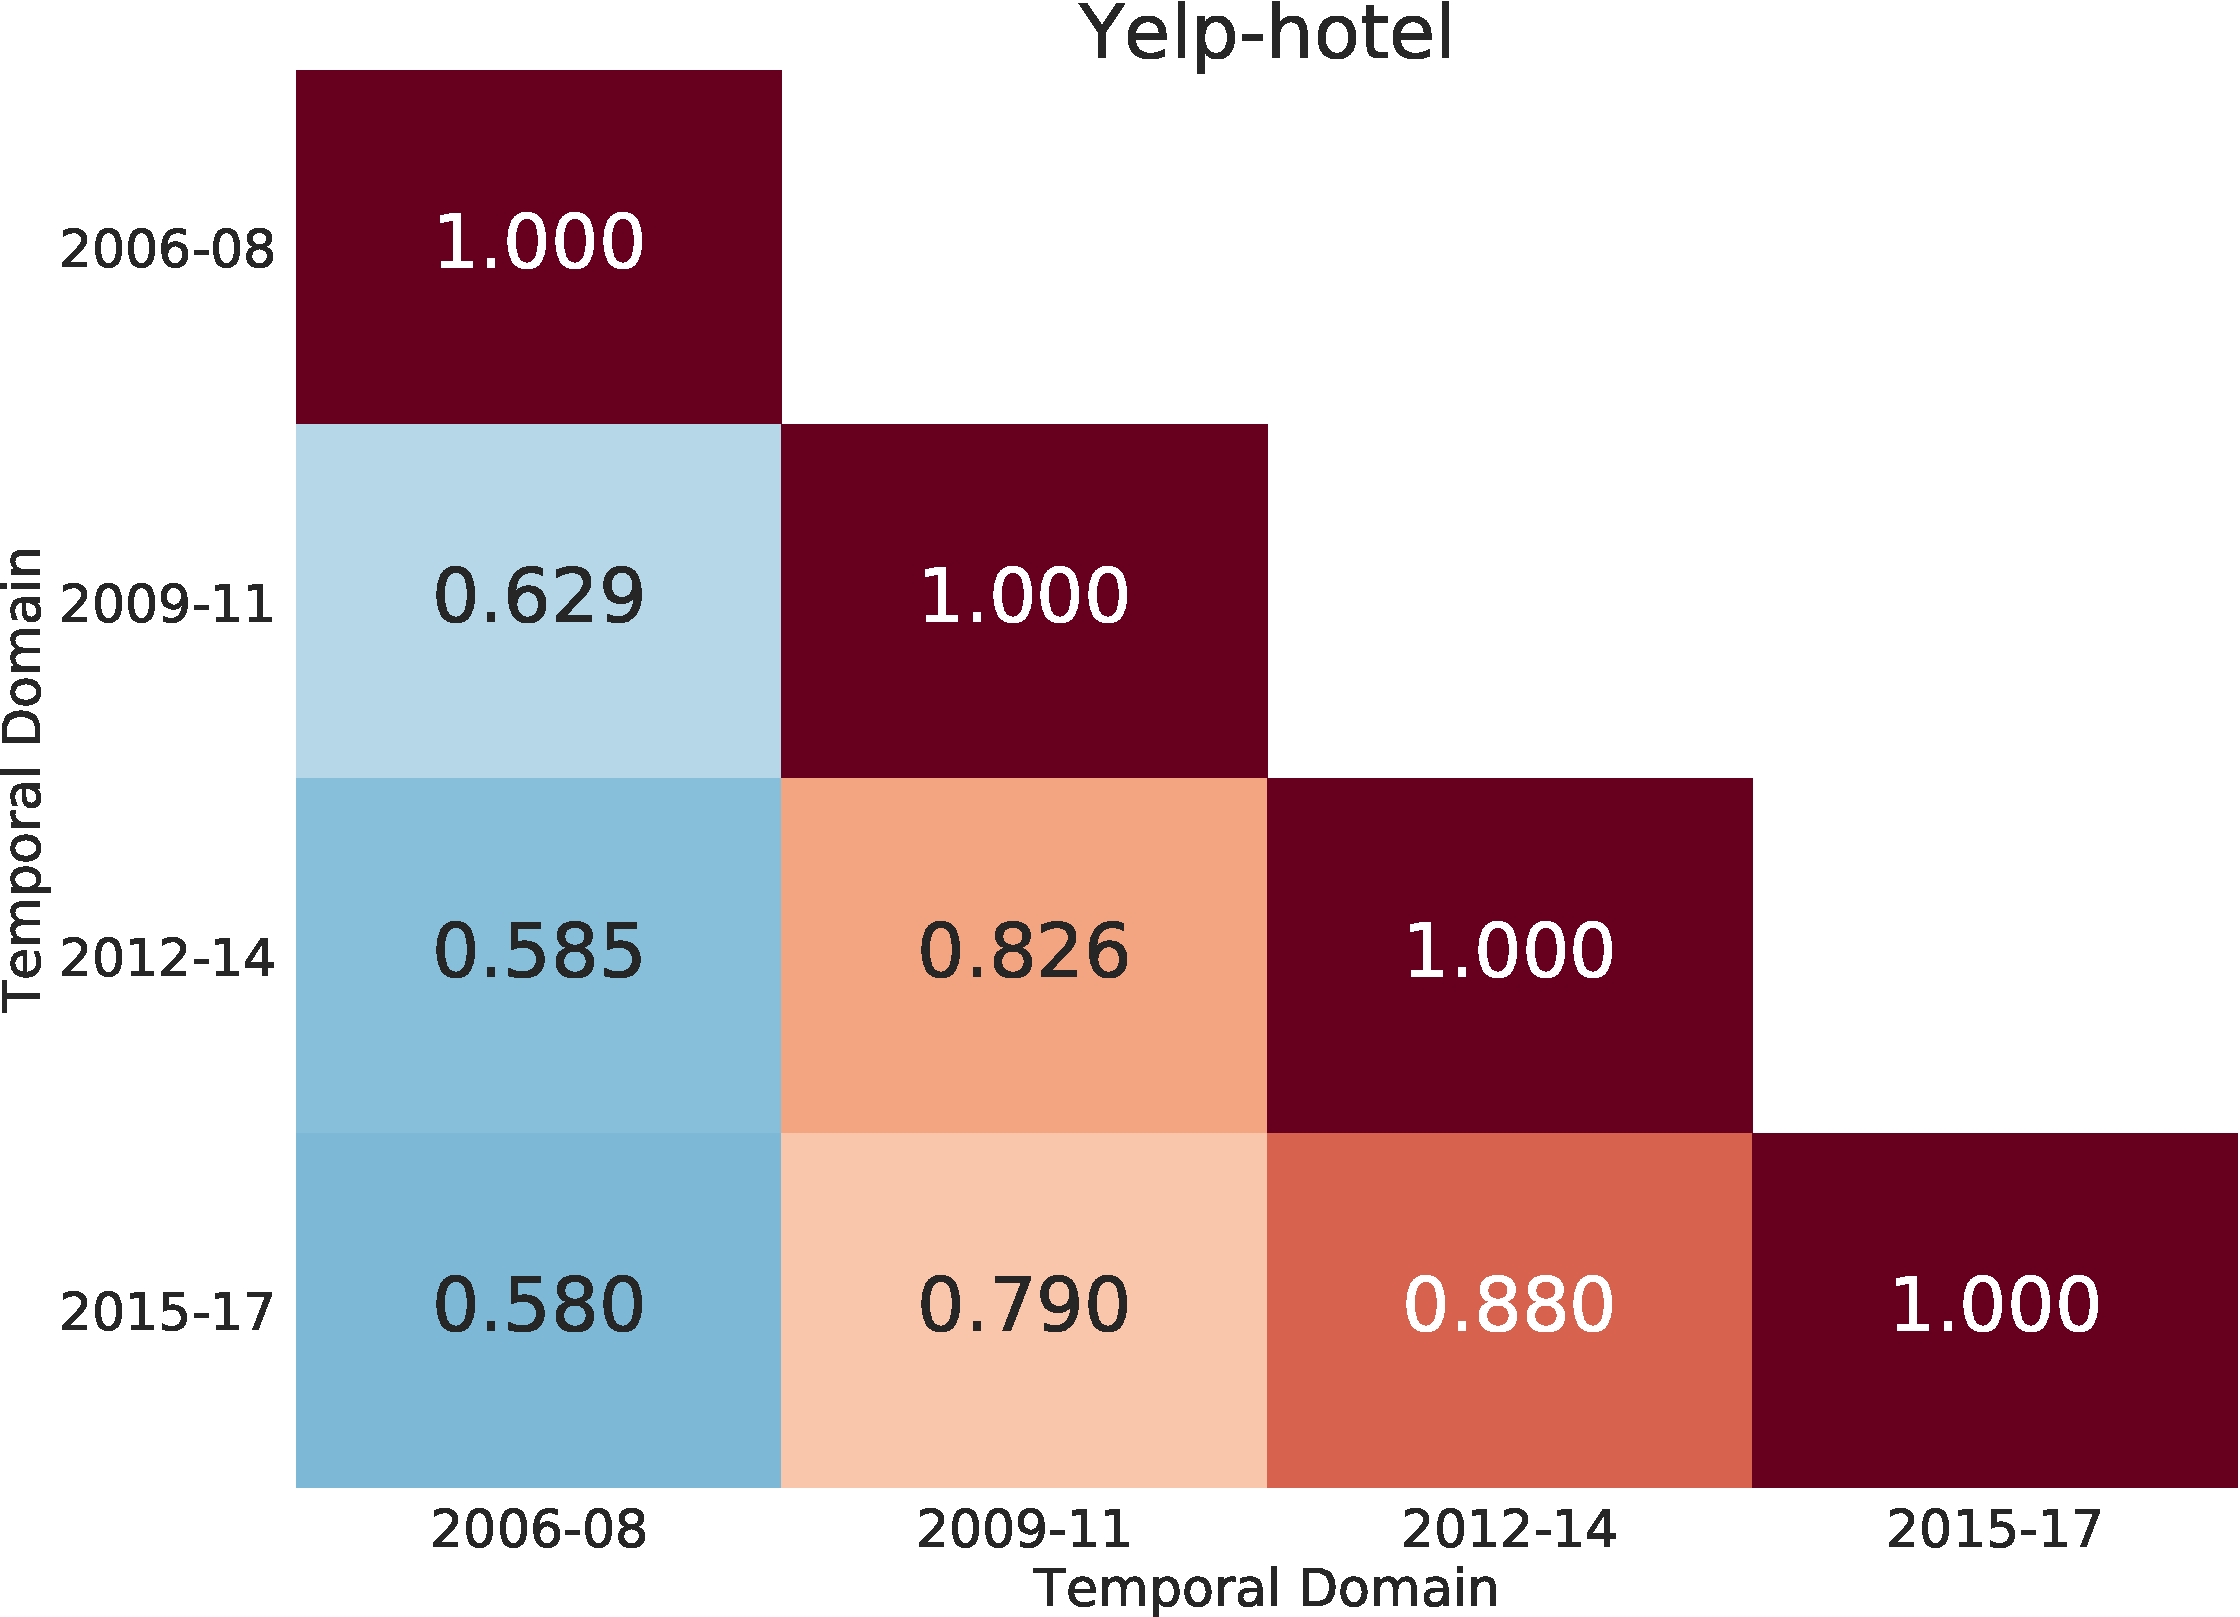
\includegraphics[width=0.31\textwidth]{images/chapter3/lang_use/yelp_hotel.pdf}
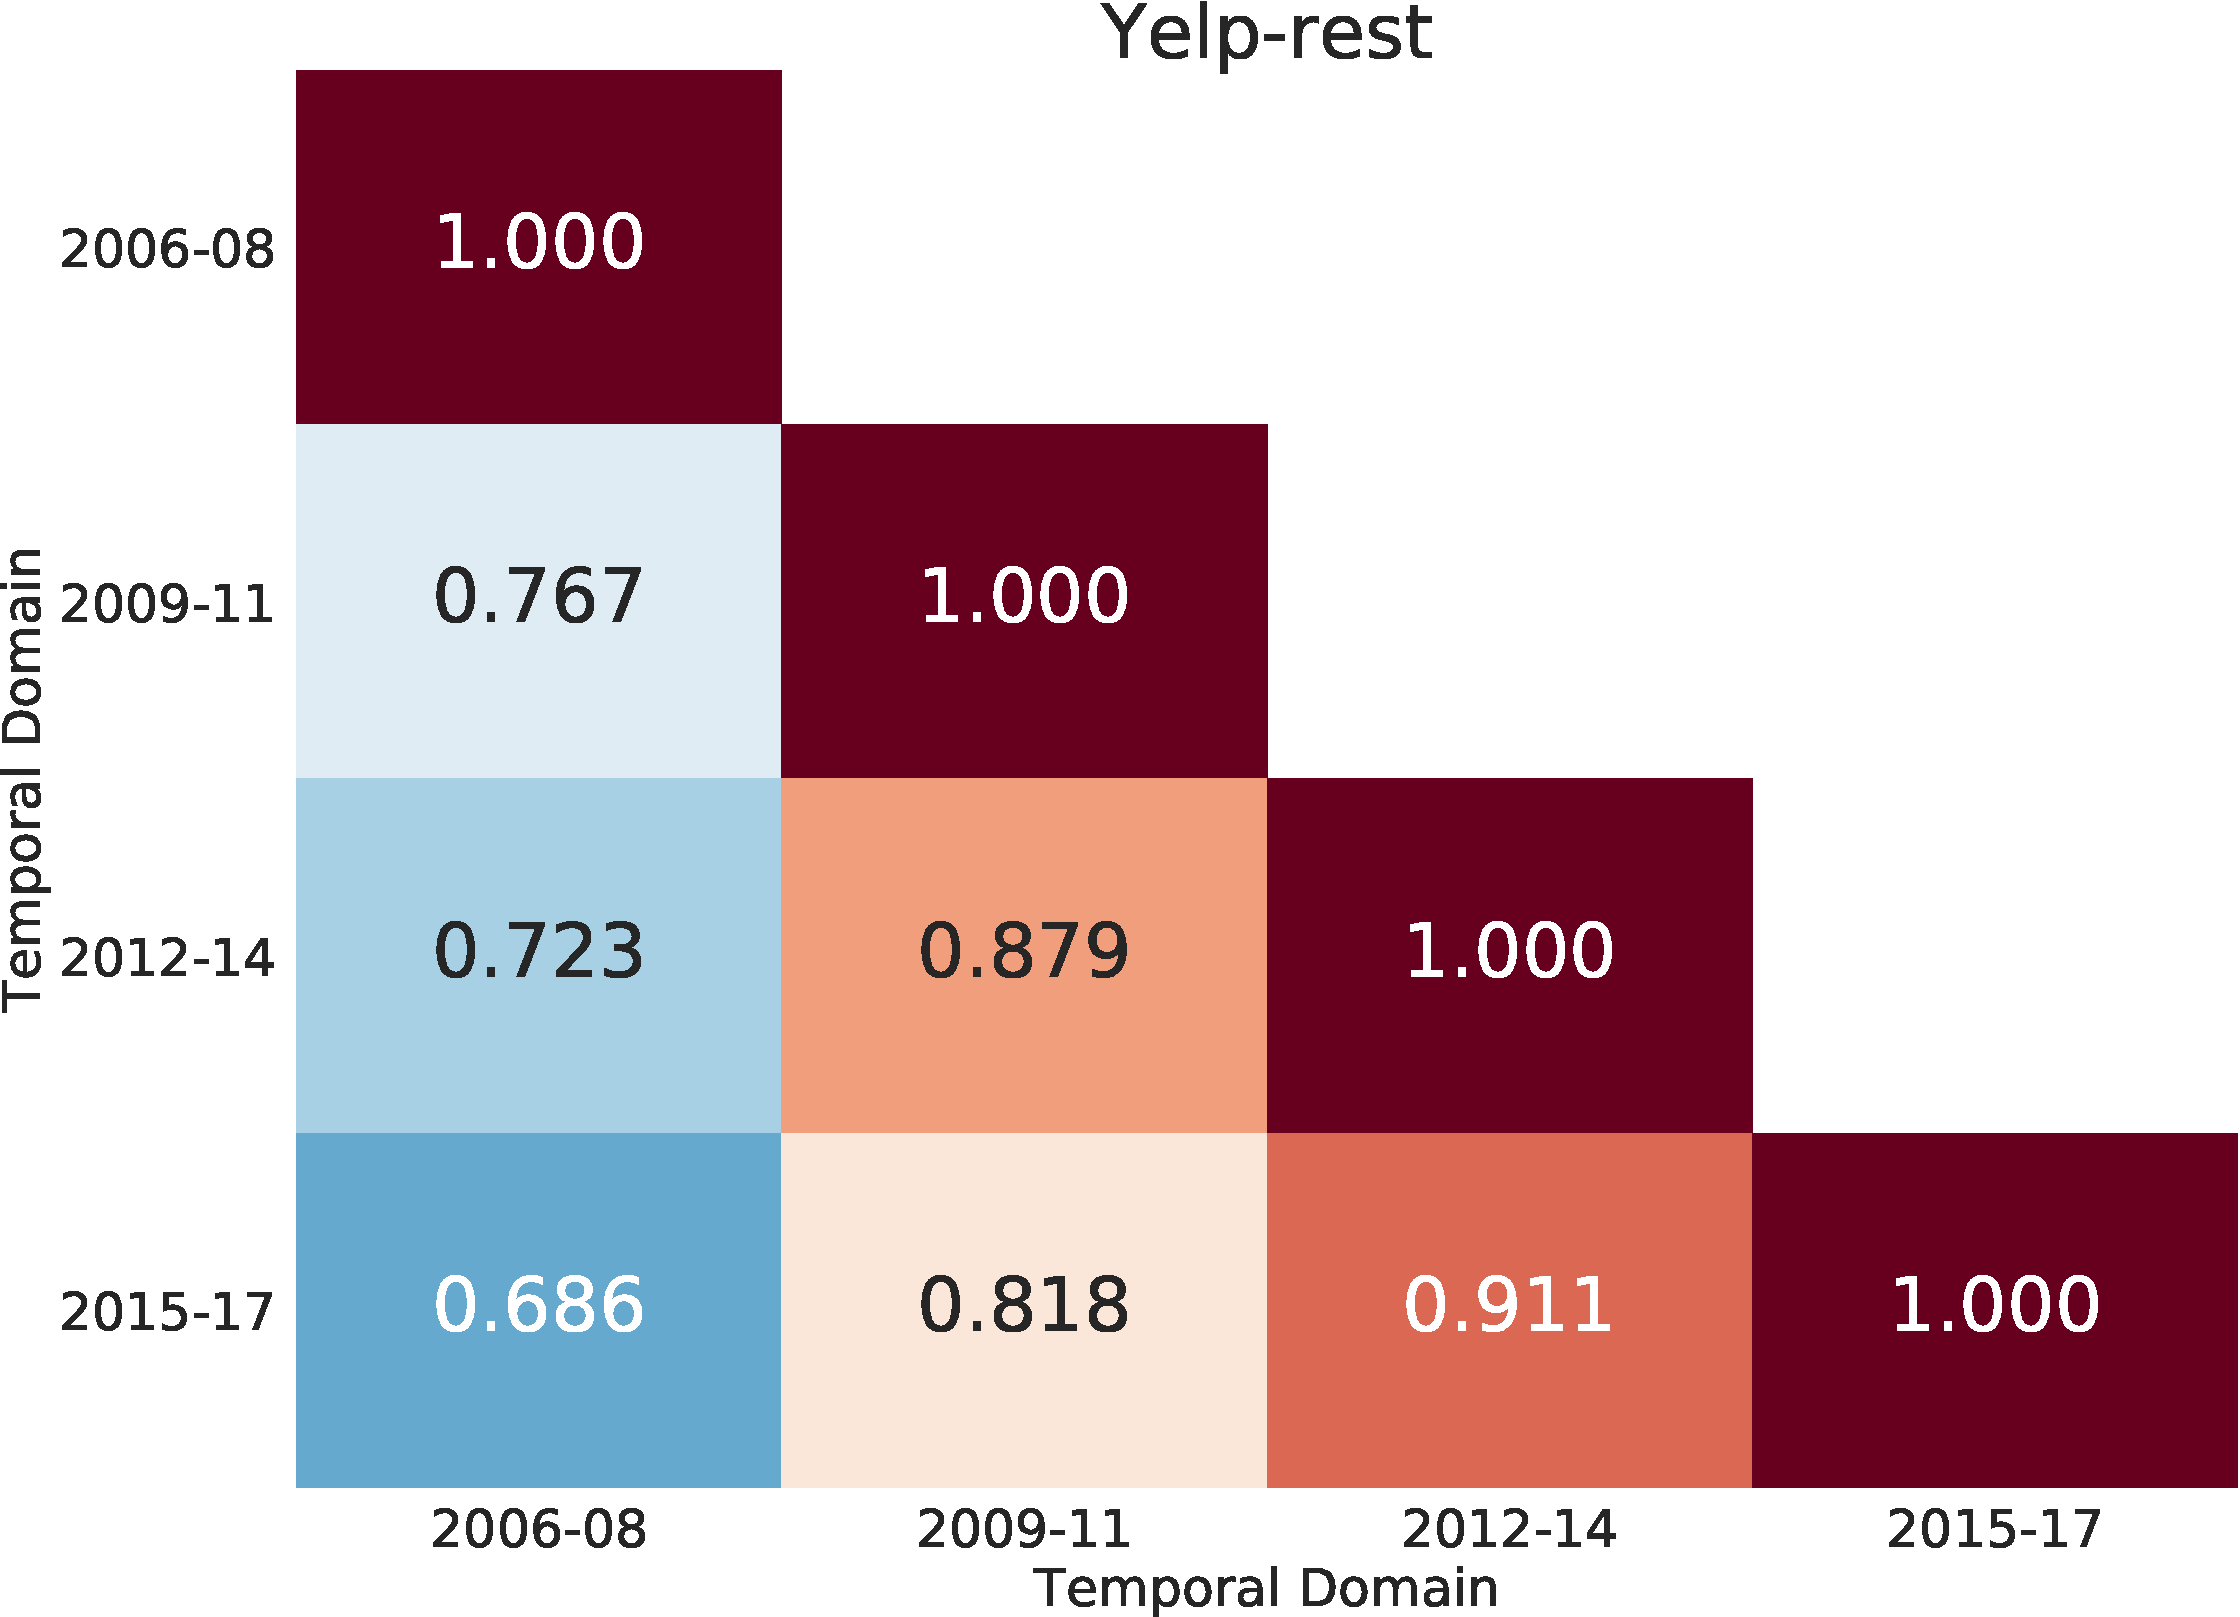
\includegraphics[width=0.31\textwidth]{images/chapter3/lang_use/yelp_rest.pdf}
\caption{Word usage overlaps between every two time domains. A value of 1 means no variations of top features between two temporal domains, while values less than 1 indicate more temporal variations.}
\label{chap3:fig:lang}
\end{figure}

Document classification models often use feature representations that are derived from words. Therefore, variations in word usage across time will change the distribution of features over time, which can impact the stability of document classifiers~\cite{huang2018examining}. 
Our goal in this section is to test whether there are temporal variations in our datasets, how strong the effects are, and what patterns exist of word usage shifts. This will help us understand how word usage variations can affect document classifiers.

We consider the word usage as it relates to document classification by measuring the overlap of top word features across time intervals. We rank and select the top 1,000 features for each interval by mutual information. We then calculate the intersection percentage between every two domains; 
specifically, if $S_0$ is the set of top features for one temporal domain and $S_1$ is the set of top features for another attribute, the percent overlap is calculated as $|S_0 \cap S_1|/1000$.

We present the overlaps of word usages across time in Figure~\ref{chap3:fig:lang}.
The overlap of word usage between temporal domains varies greatly across different corpora (ranging from 0.322 to 0.911). We  observe that closer temporal domains usually have higher overlap while further temporal domains share less overlap. These results thus suggest that the word usage varies over time across many settings.


\subsection{Analysis 2: Context Shift}
\label{chap3:subsec:ctt_shift}

\begin{figure}[tb!]
\centering
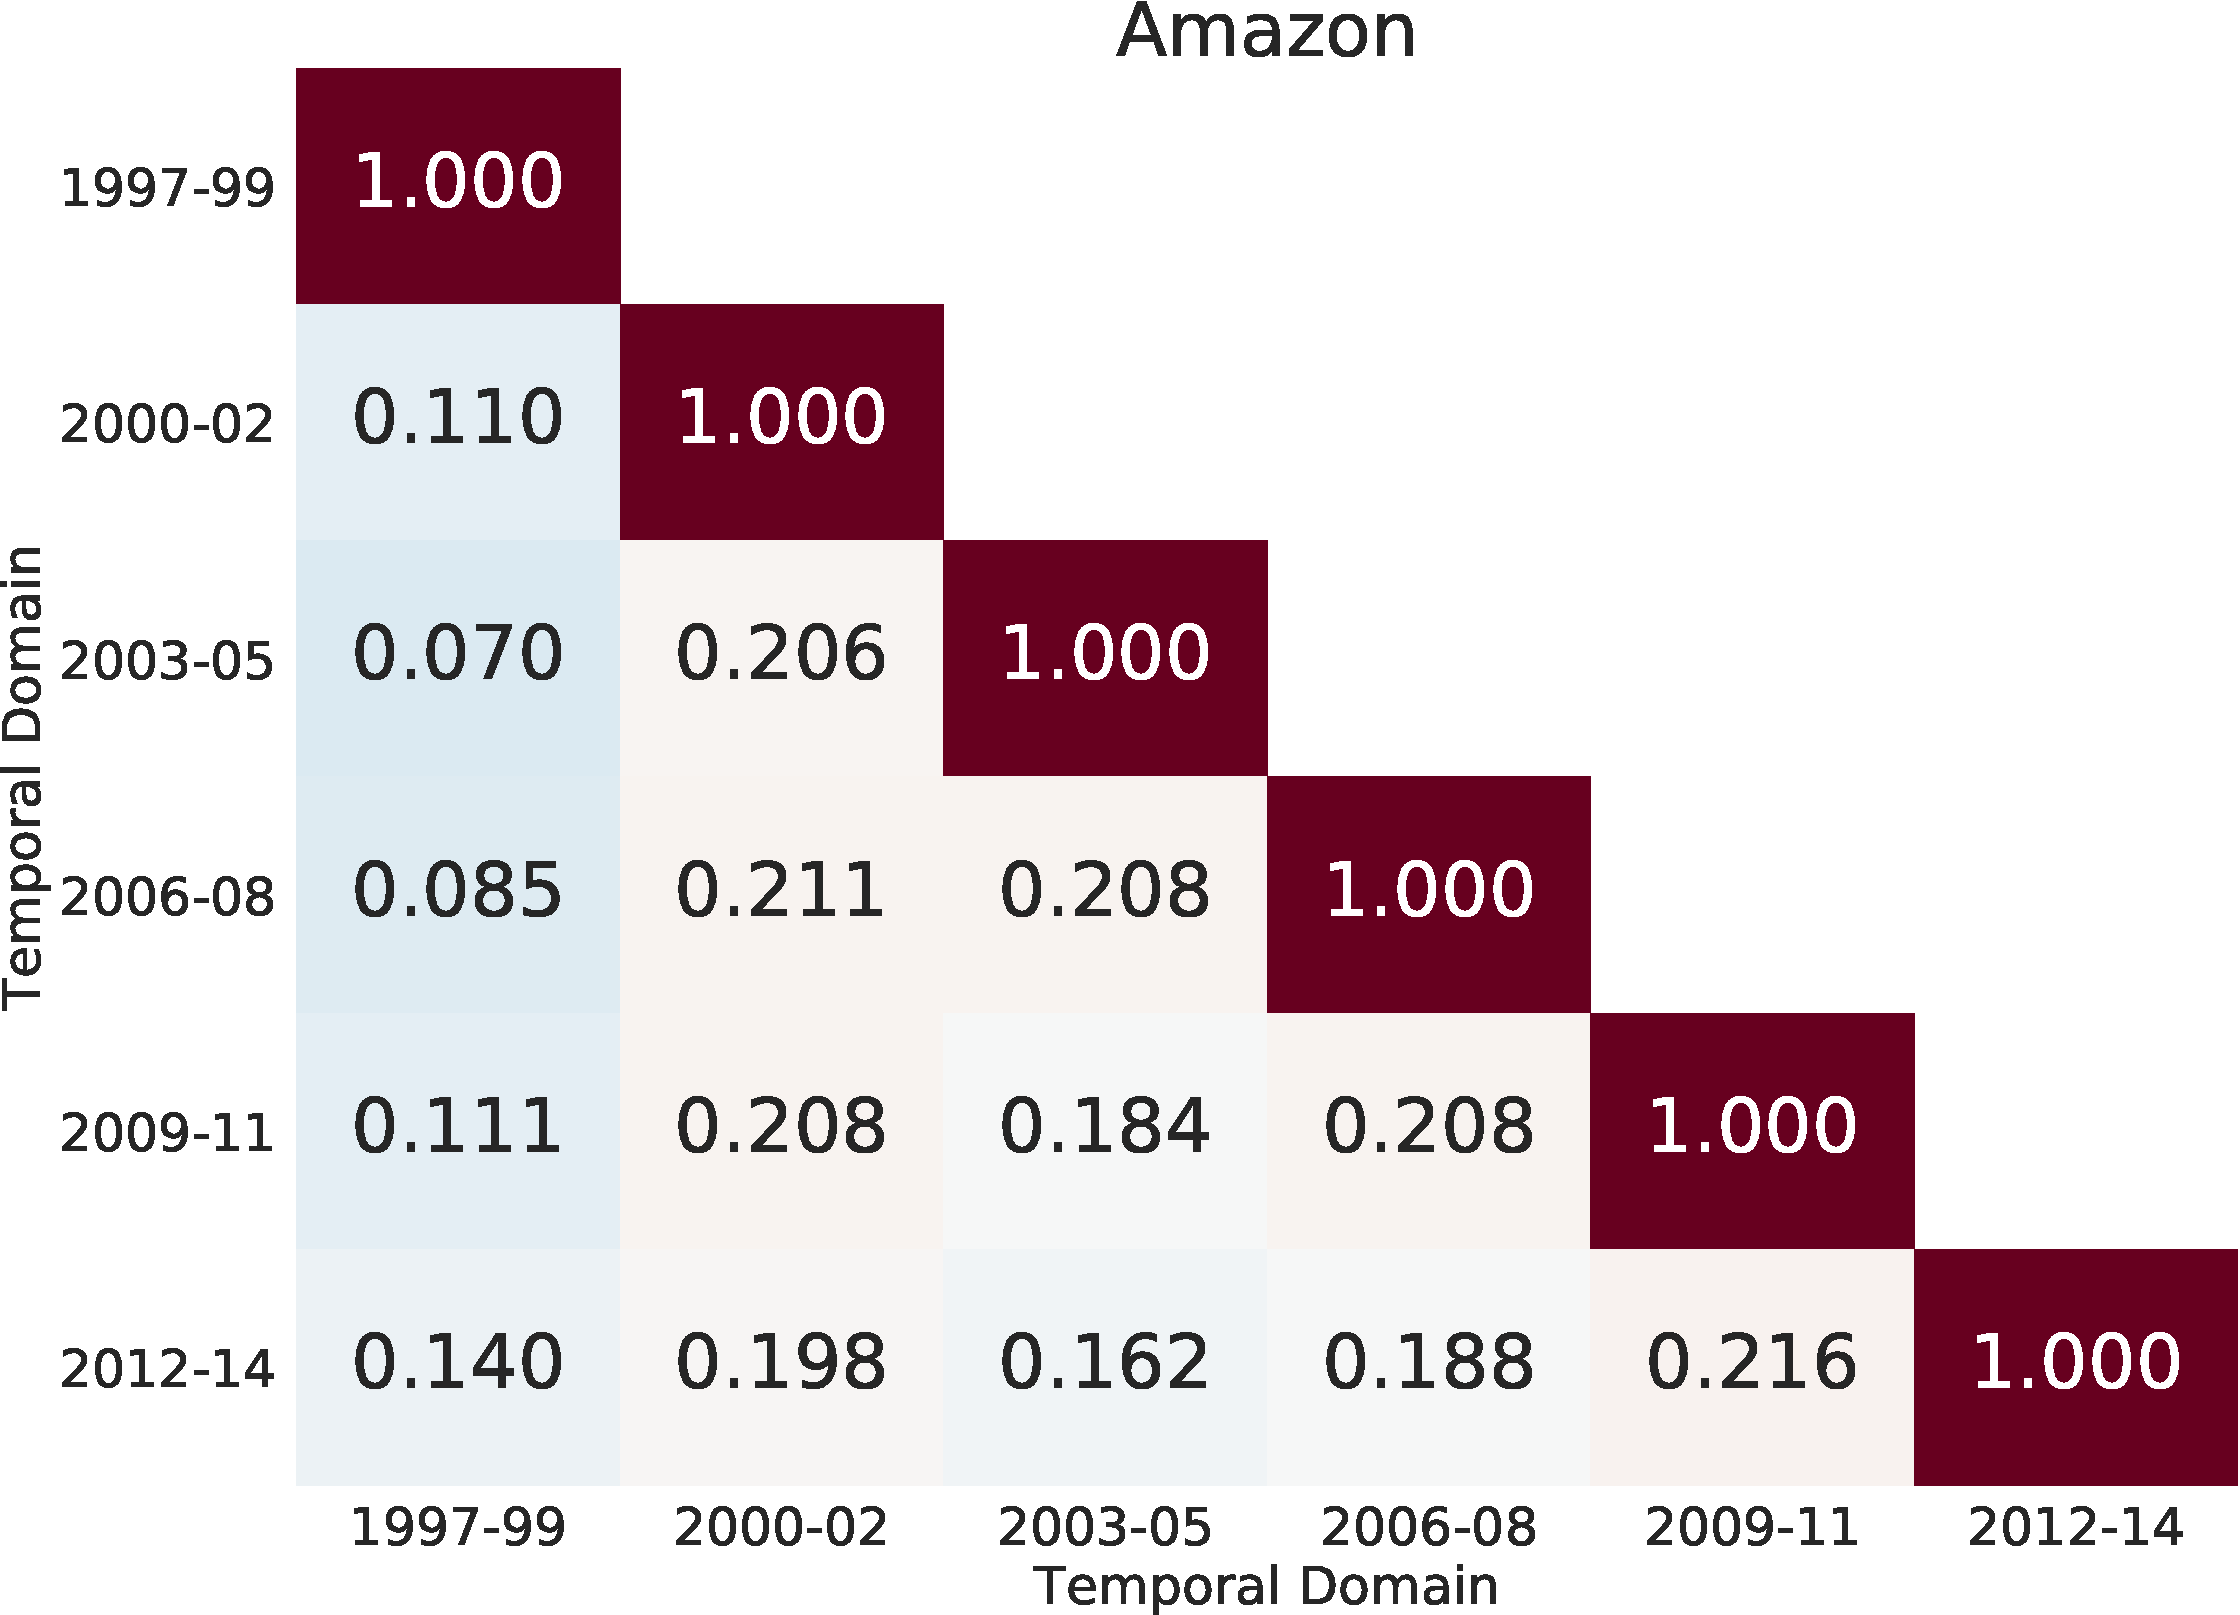
\includegraphics[width=0.31\textwidth]{images/chapter3/ctt_shift/amazon.pdf}
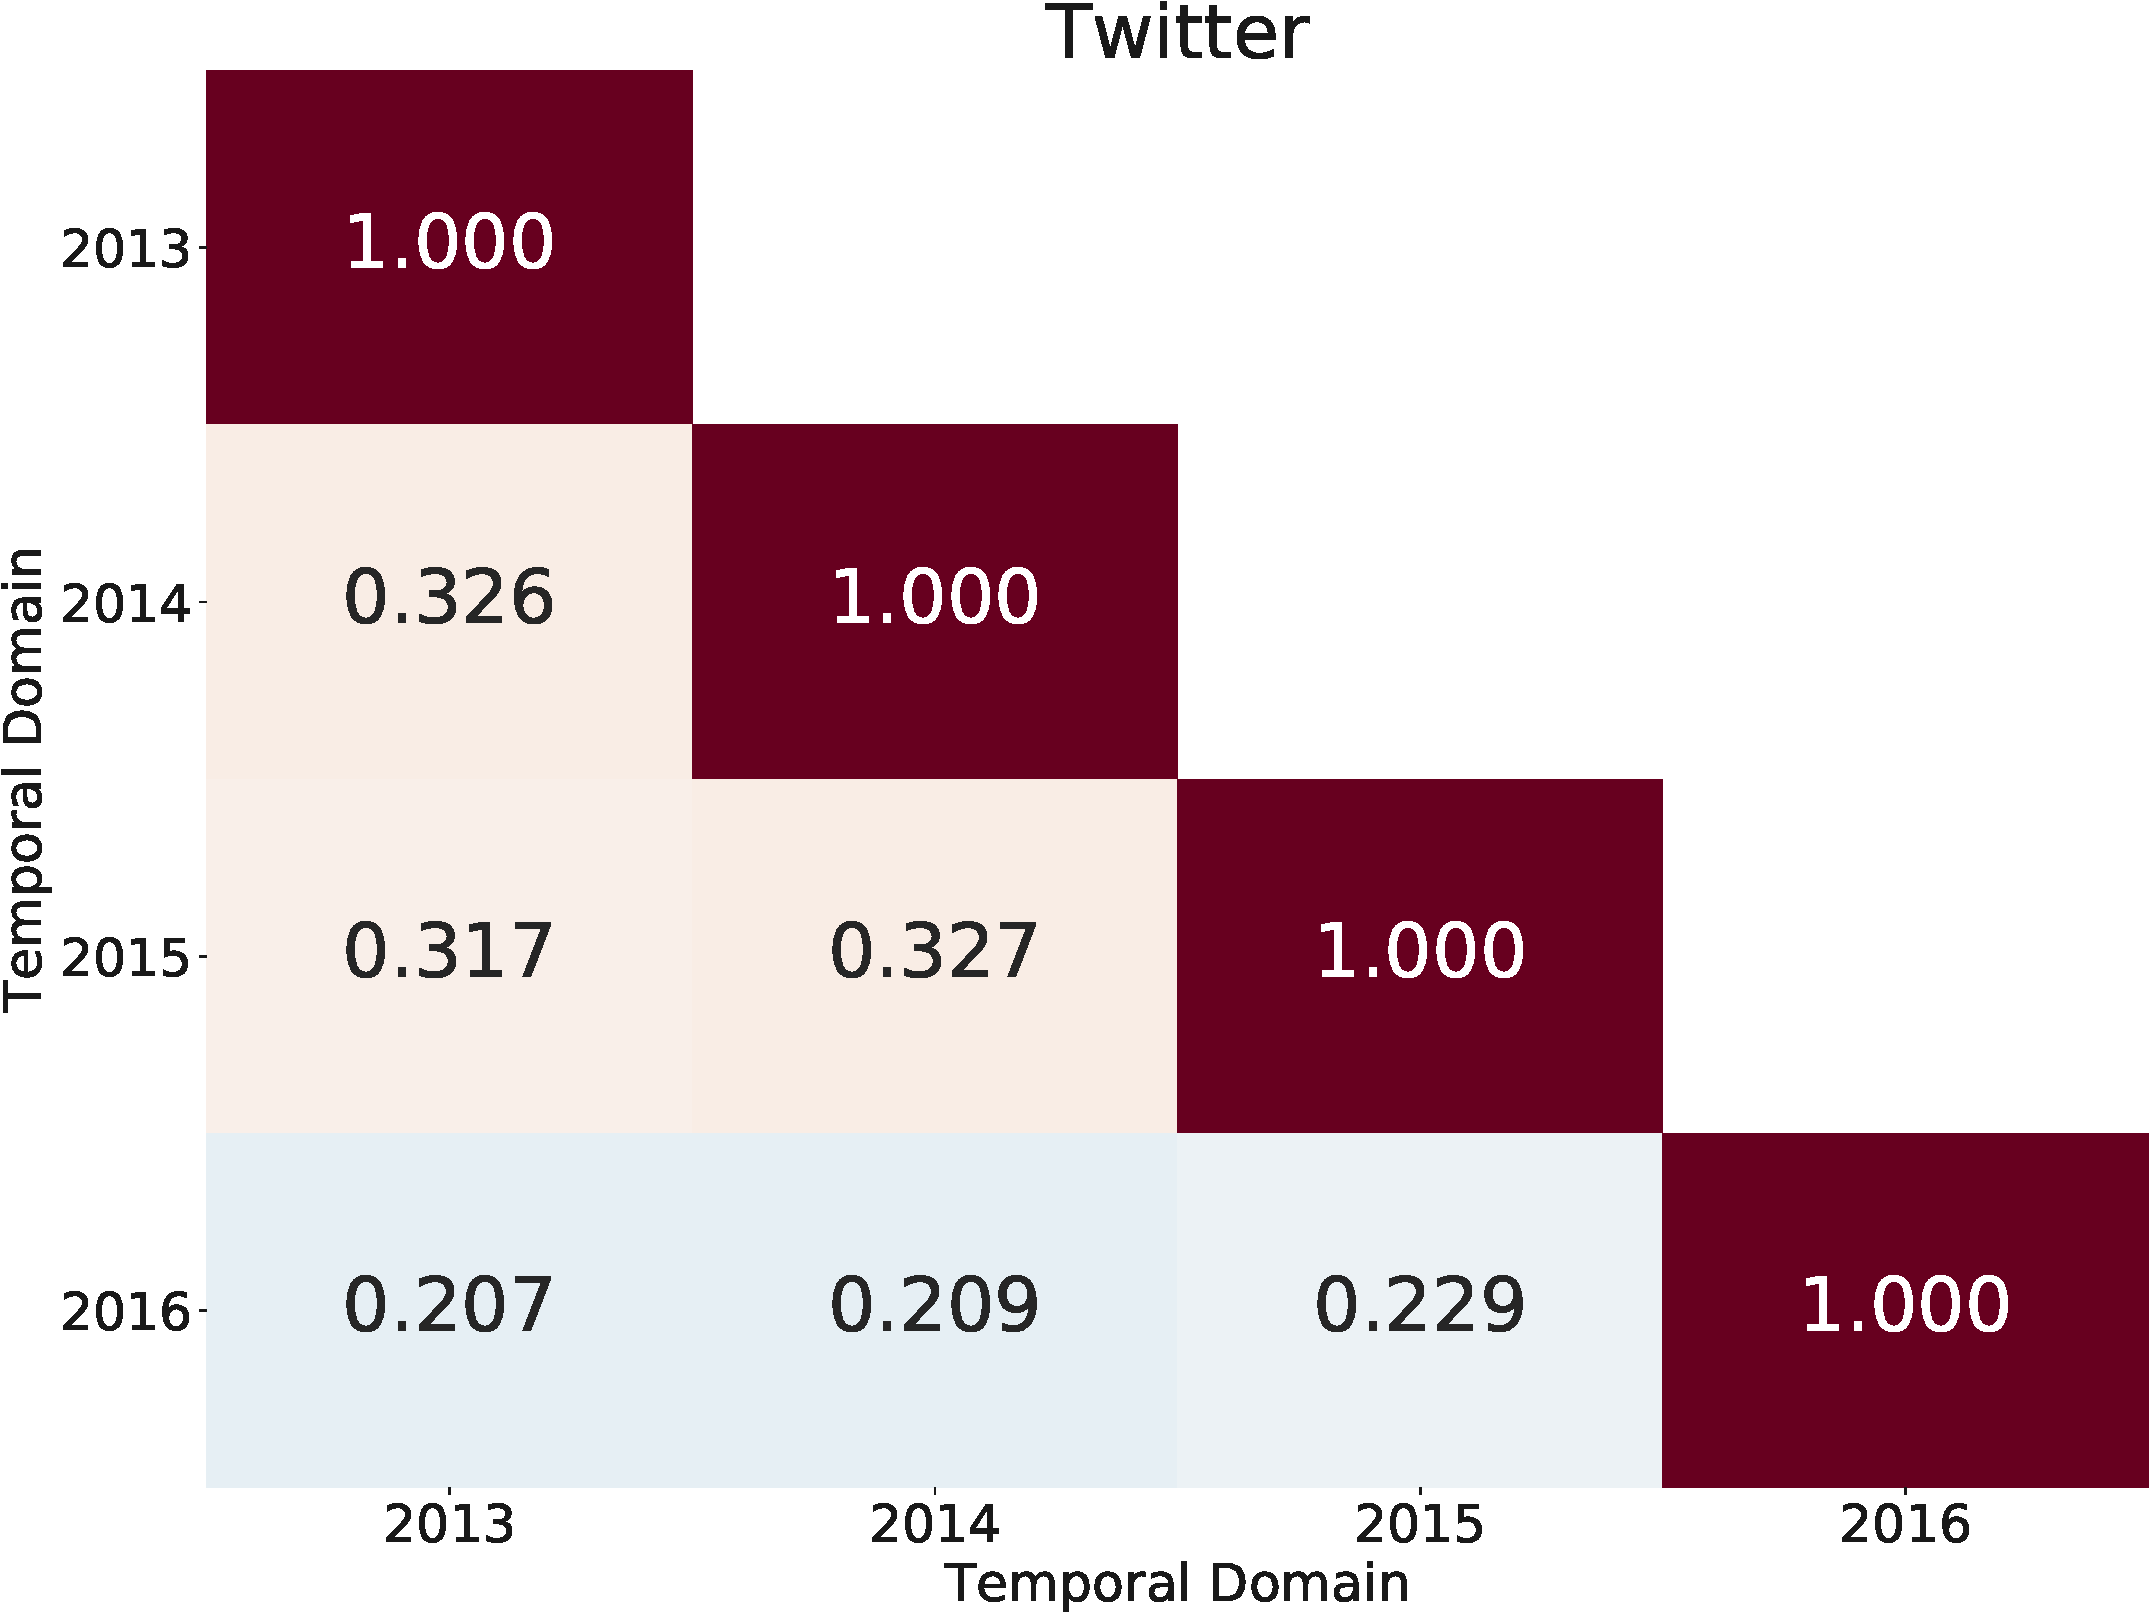
\includegraphics[width=0.31\textwidth]{images/chapter3/ctt_shift/vaccine.pdf}
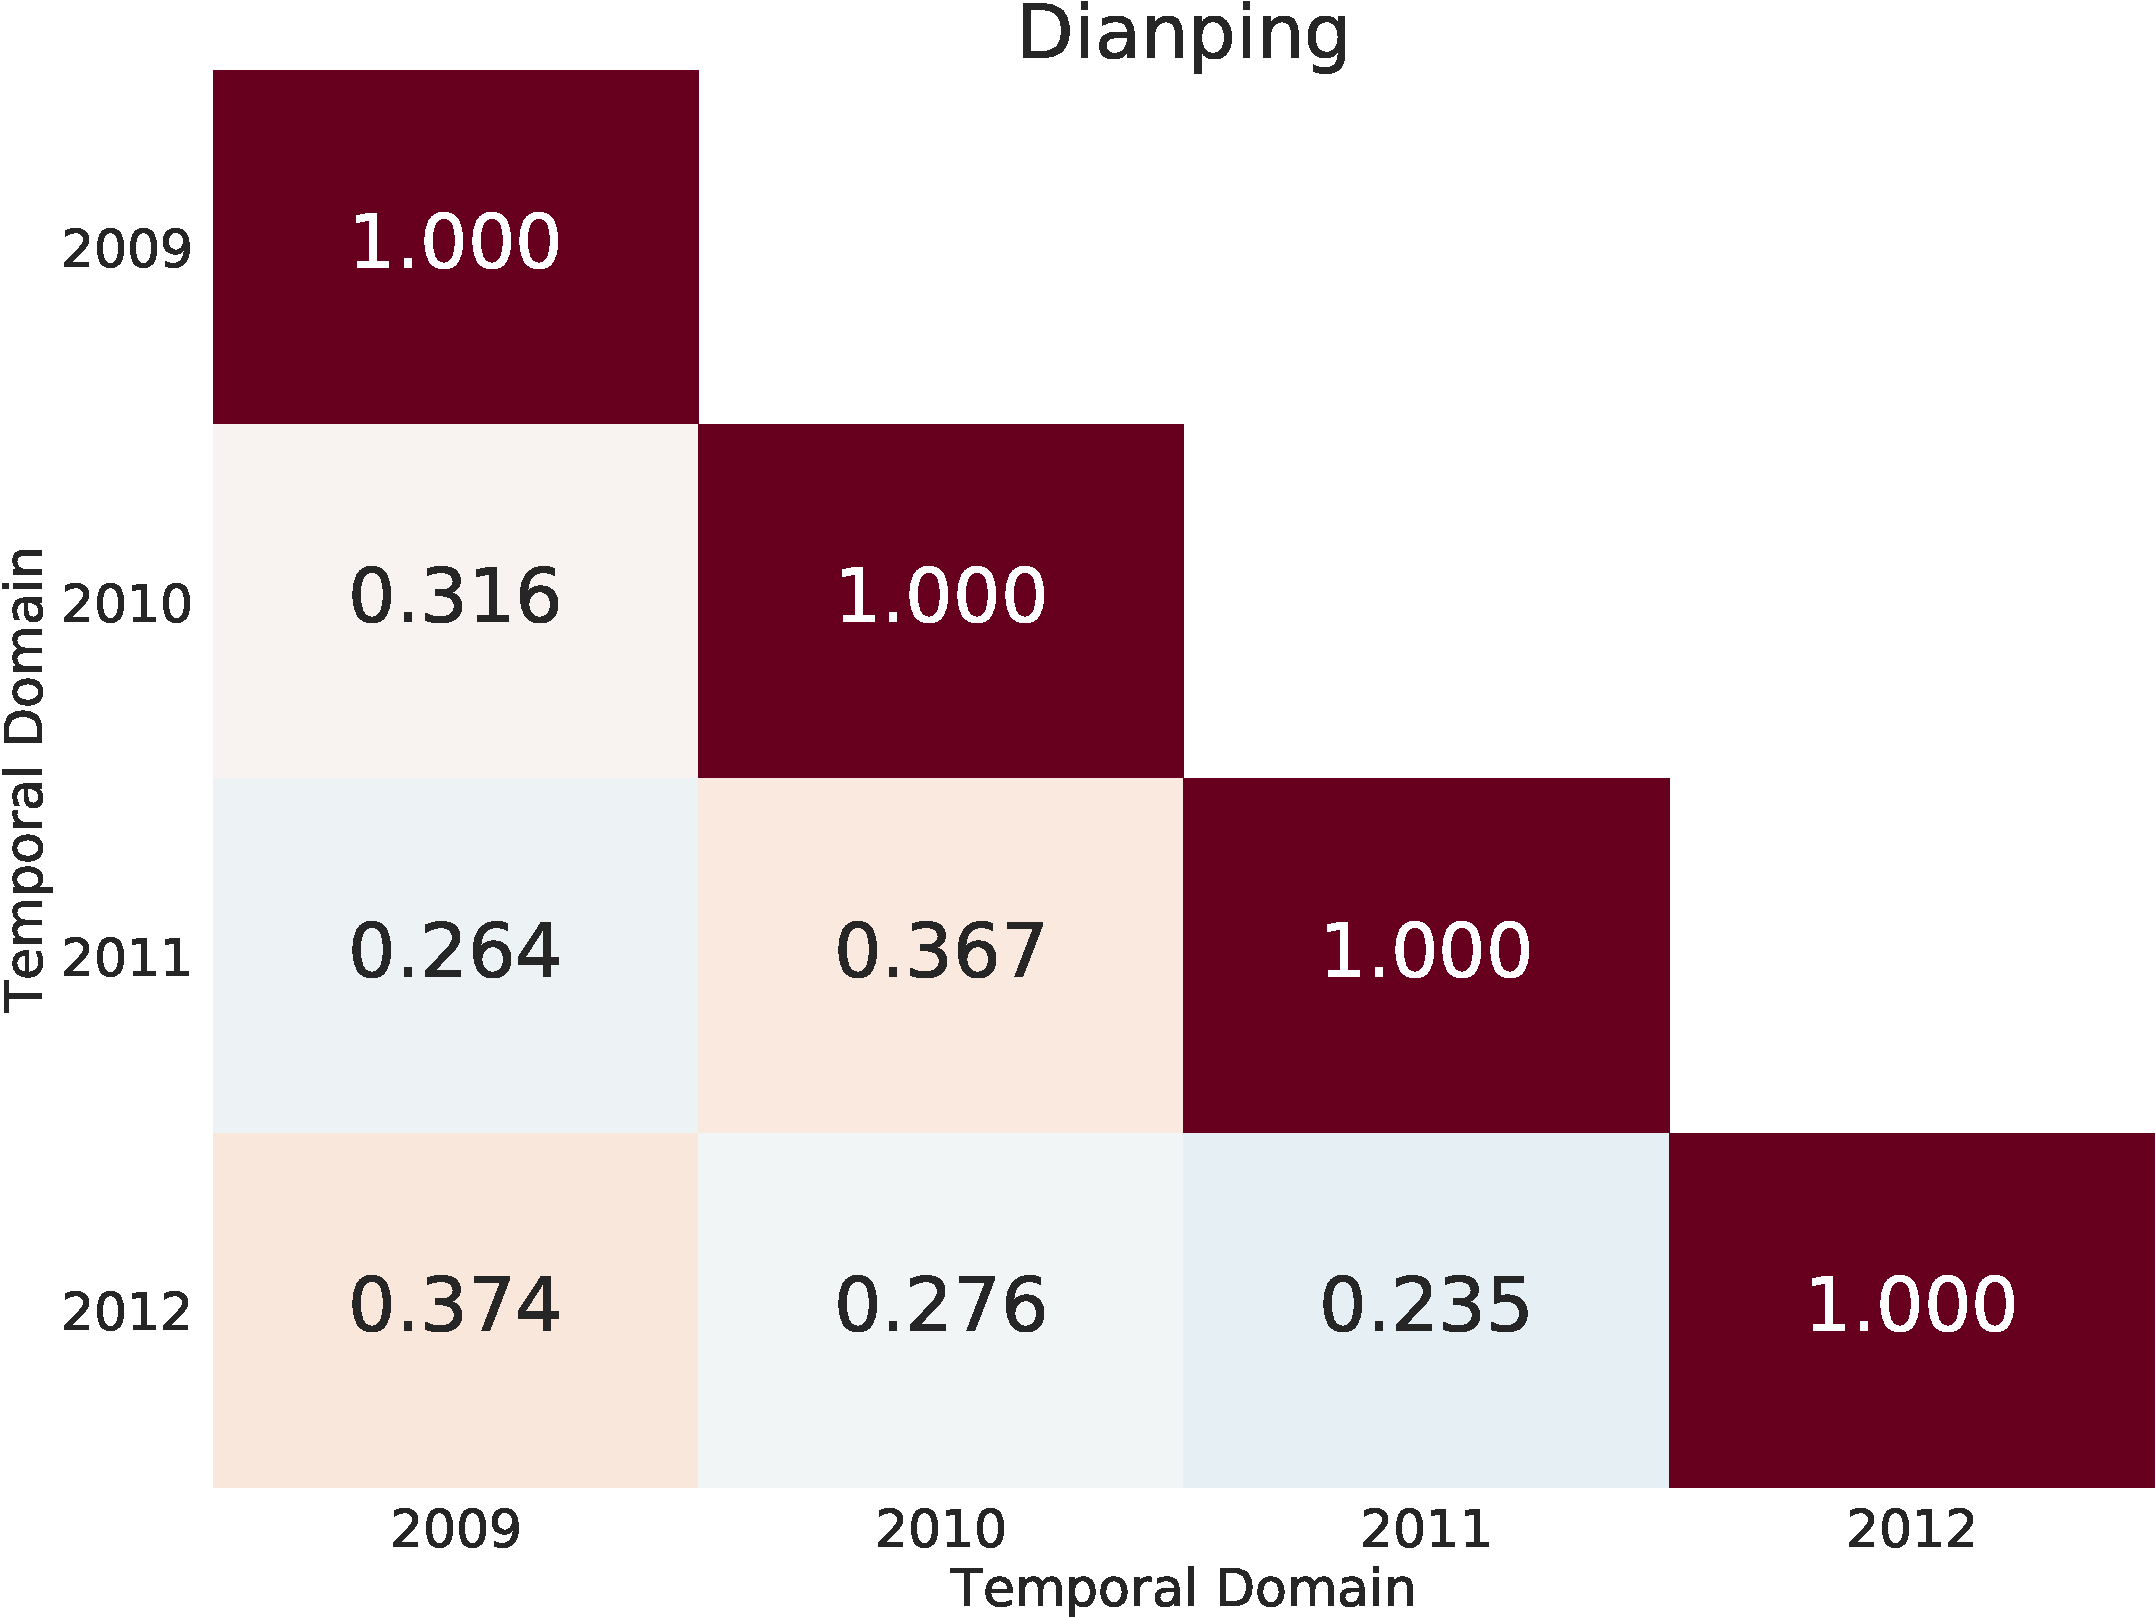
\includegraphics[width=0.31\textwidth]{images/chapter3/ctt_shift/dianping.pdf}
\newline
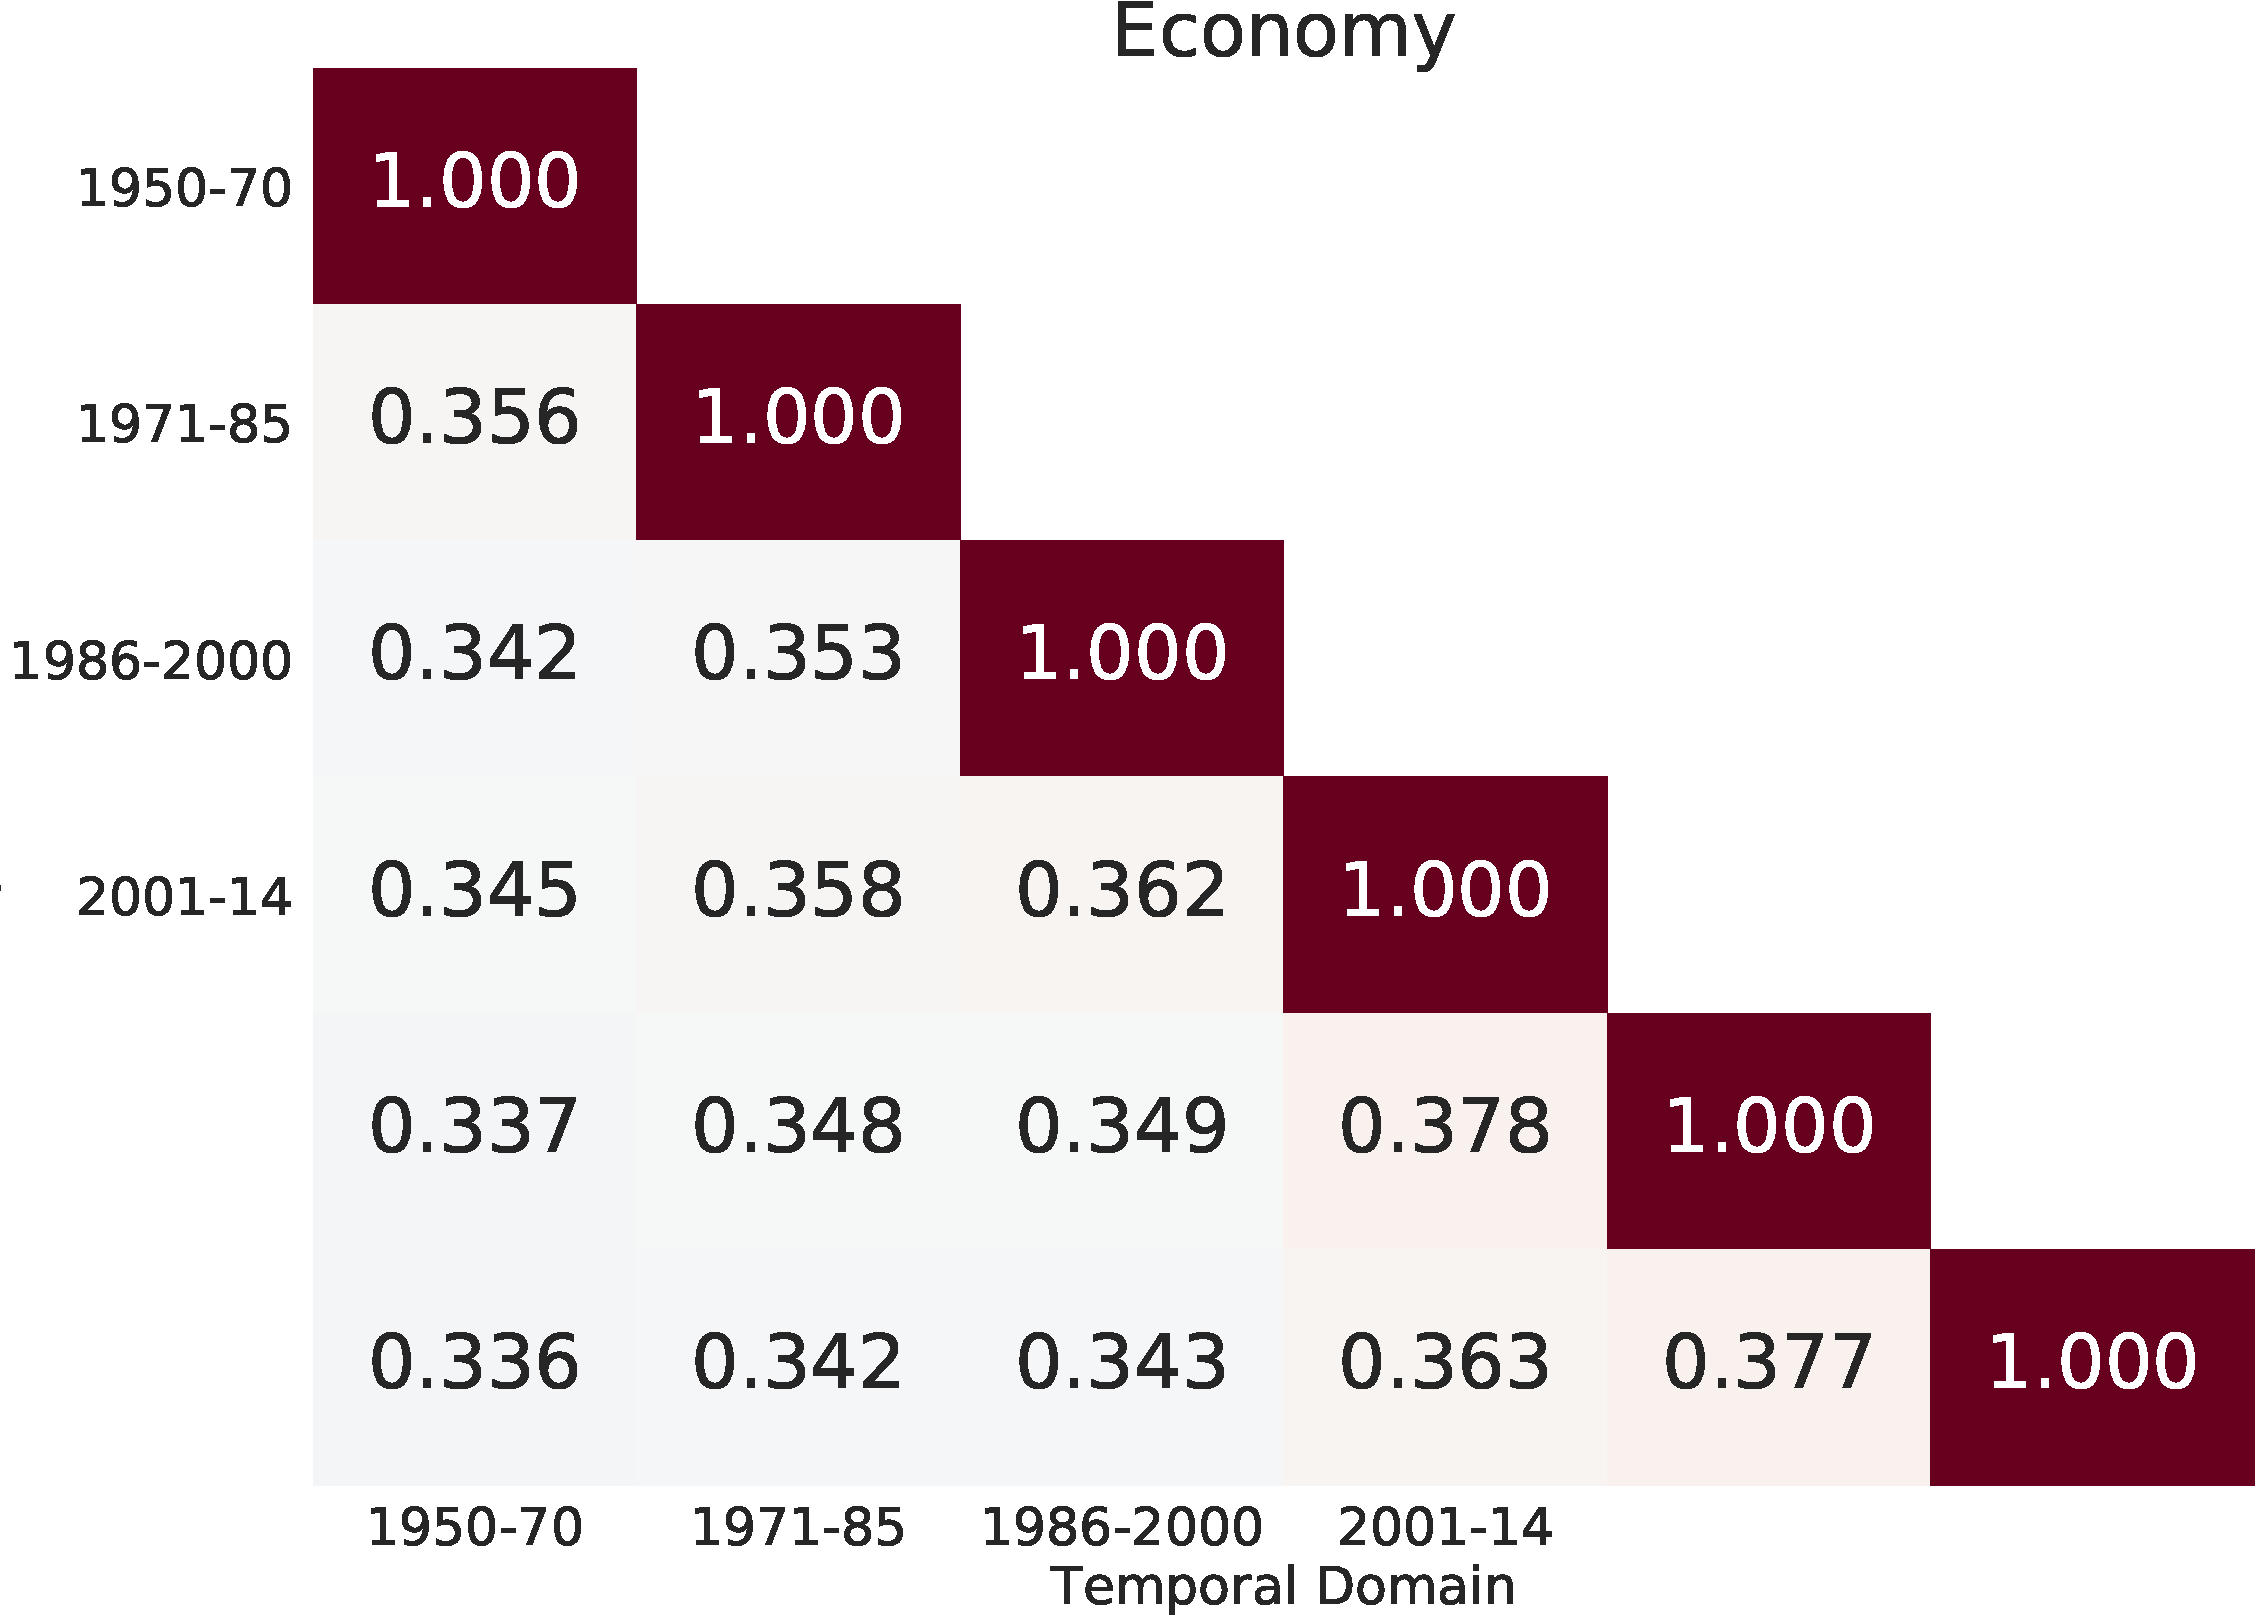
\includegraphics[width=0.31\textwidth]{images/chapter3/ctt_shift/economy.pdf}
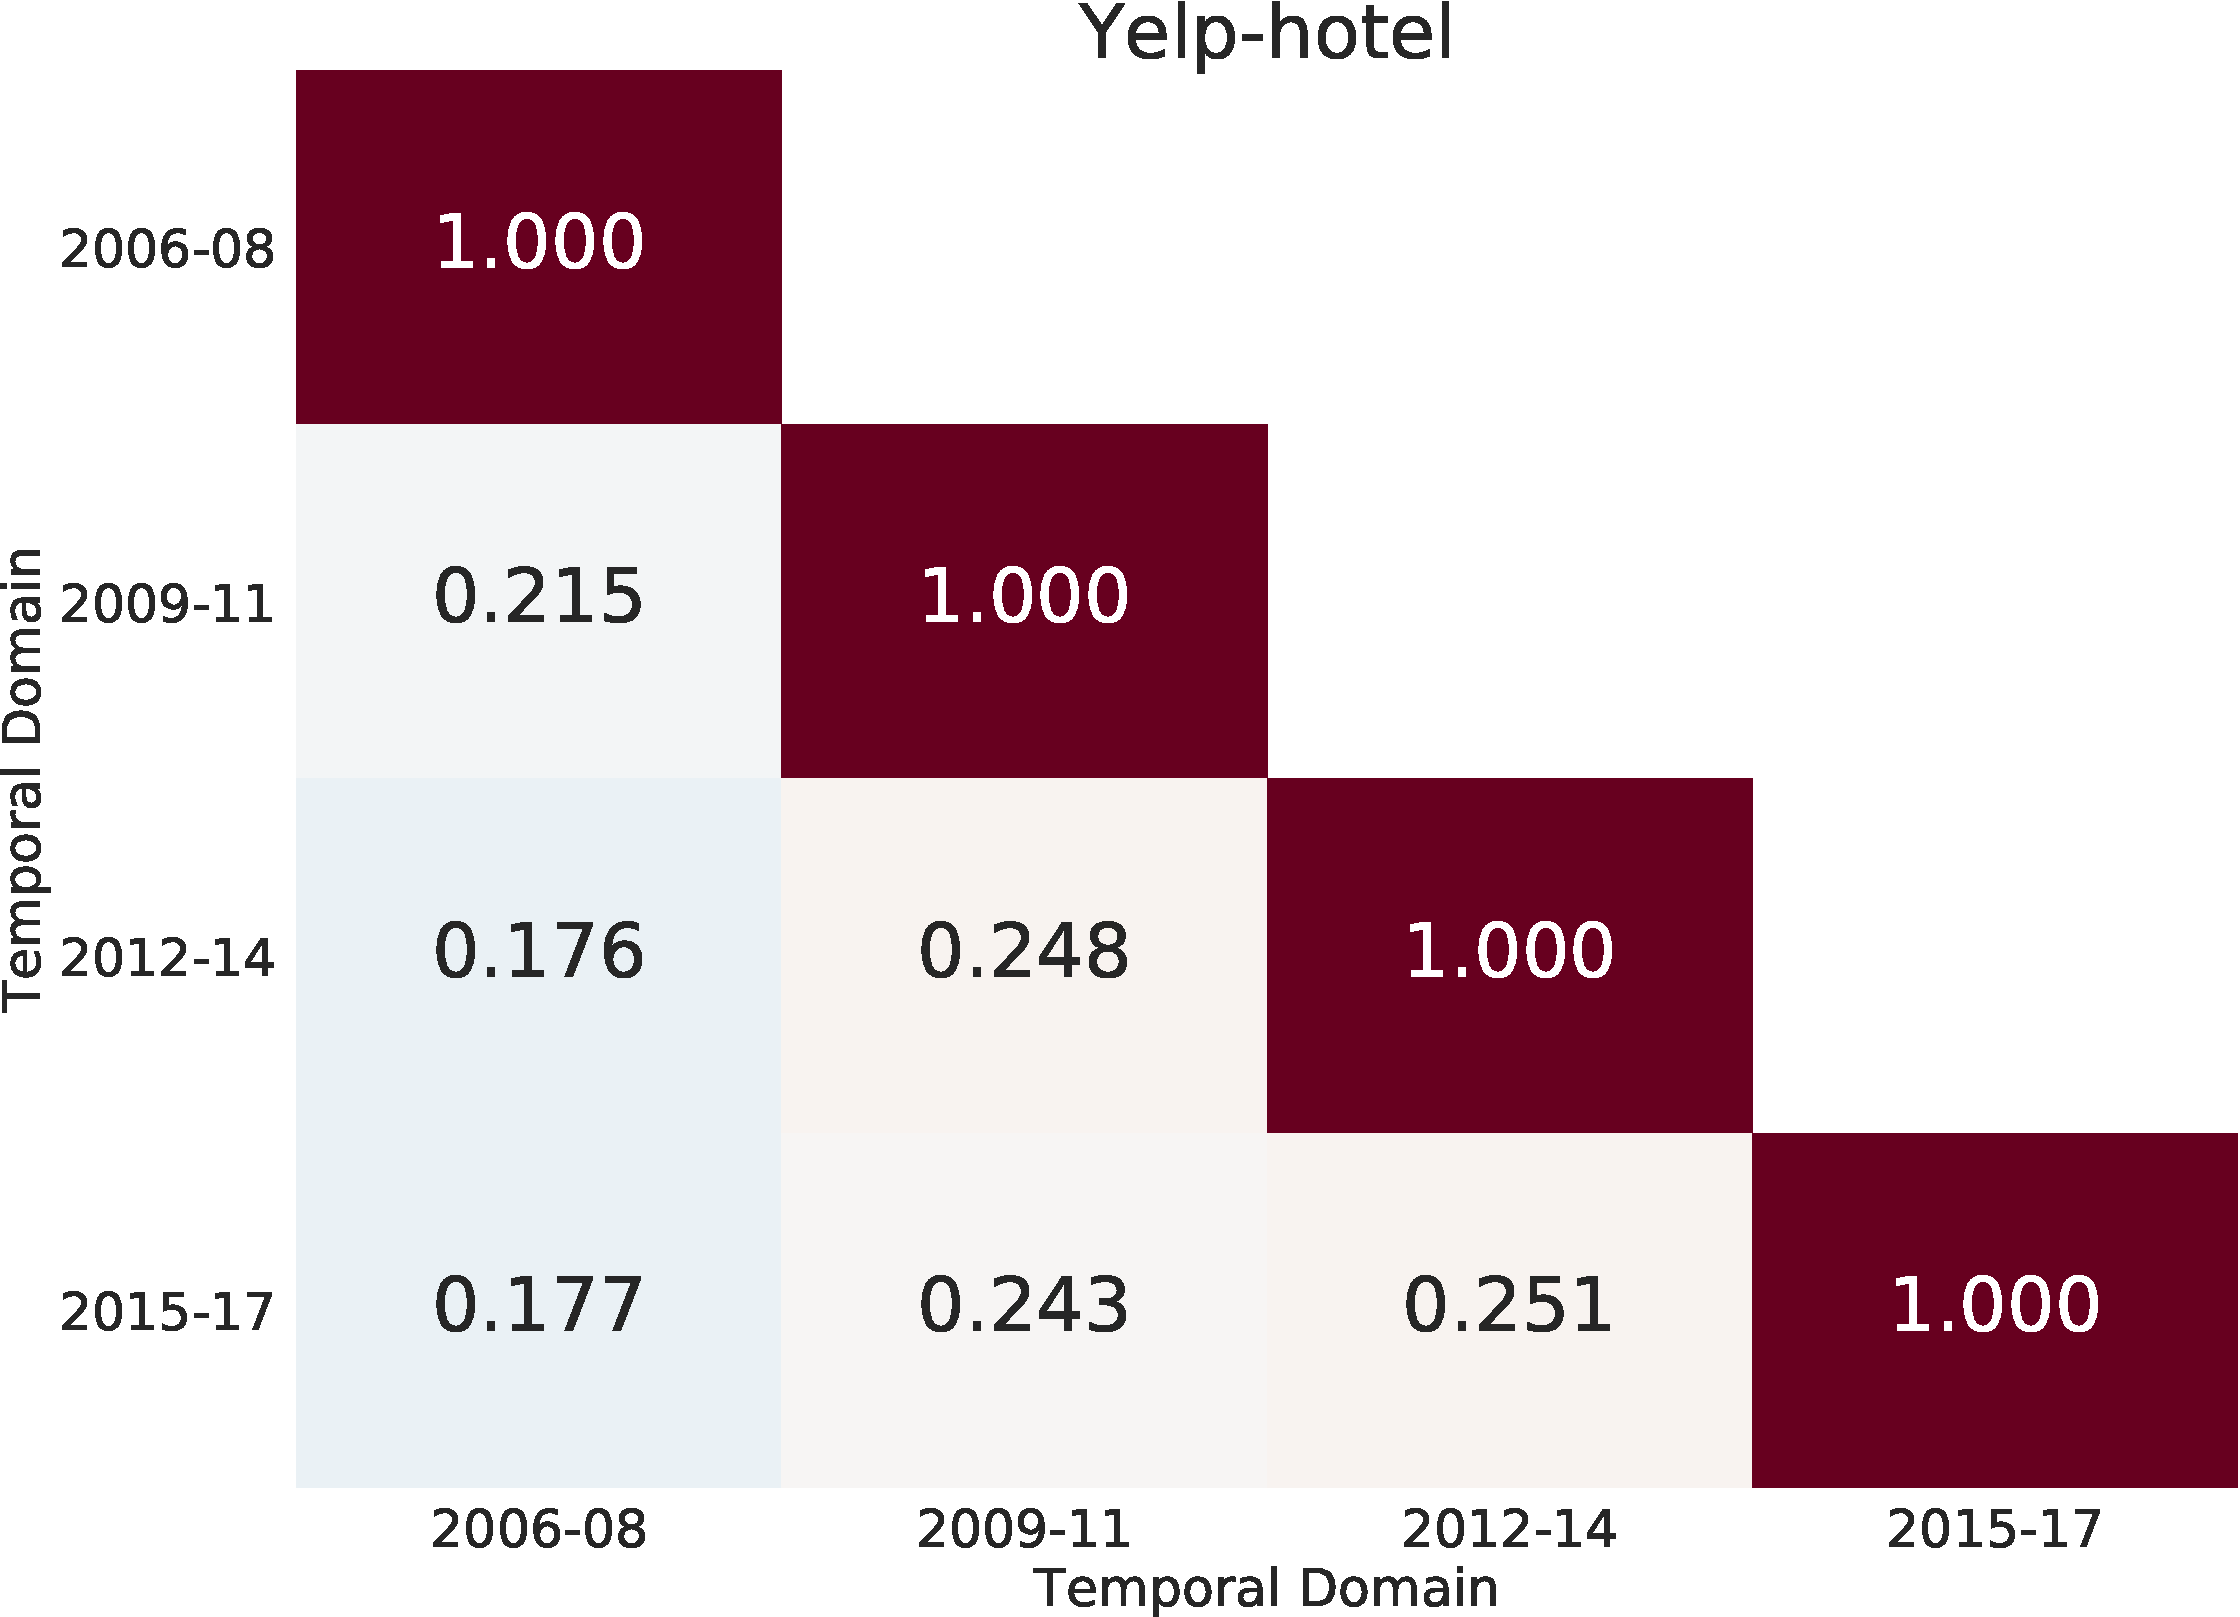
\includegraphics[width=0.31\textwidth]{images/chapter3/ctt_shift/yelp_hotel.pdf}
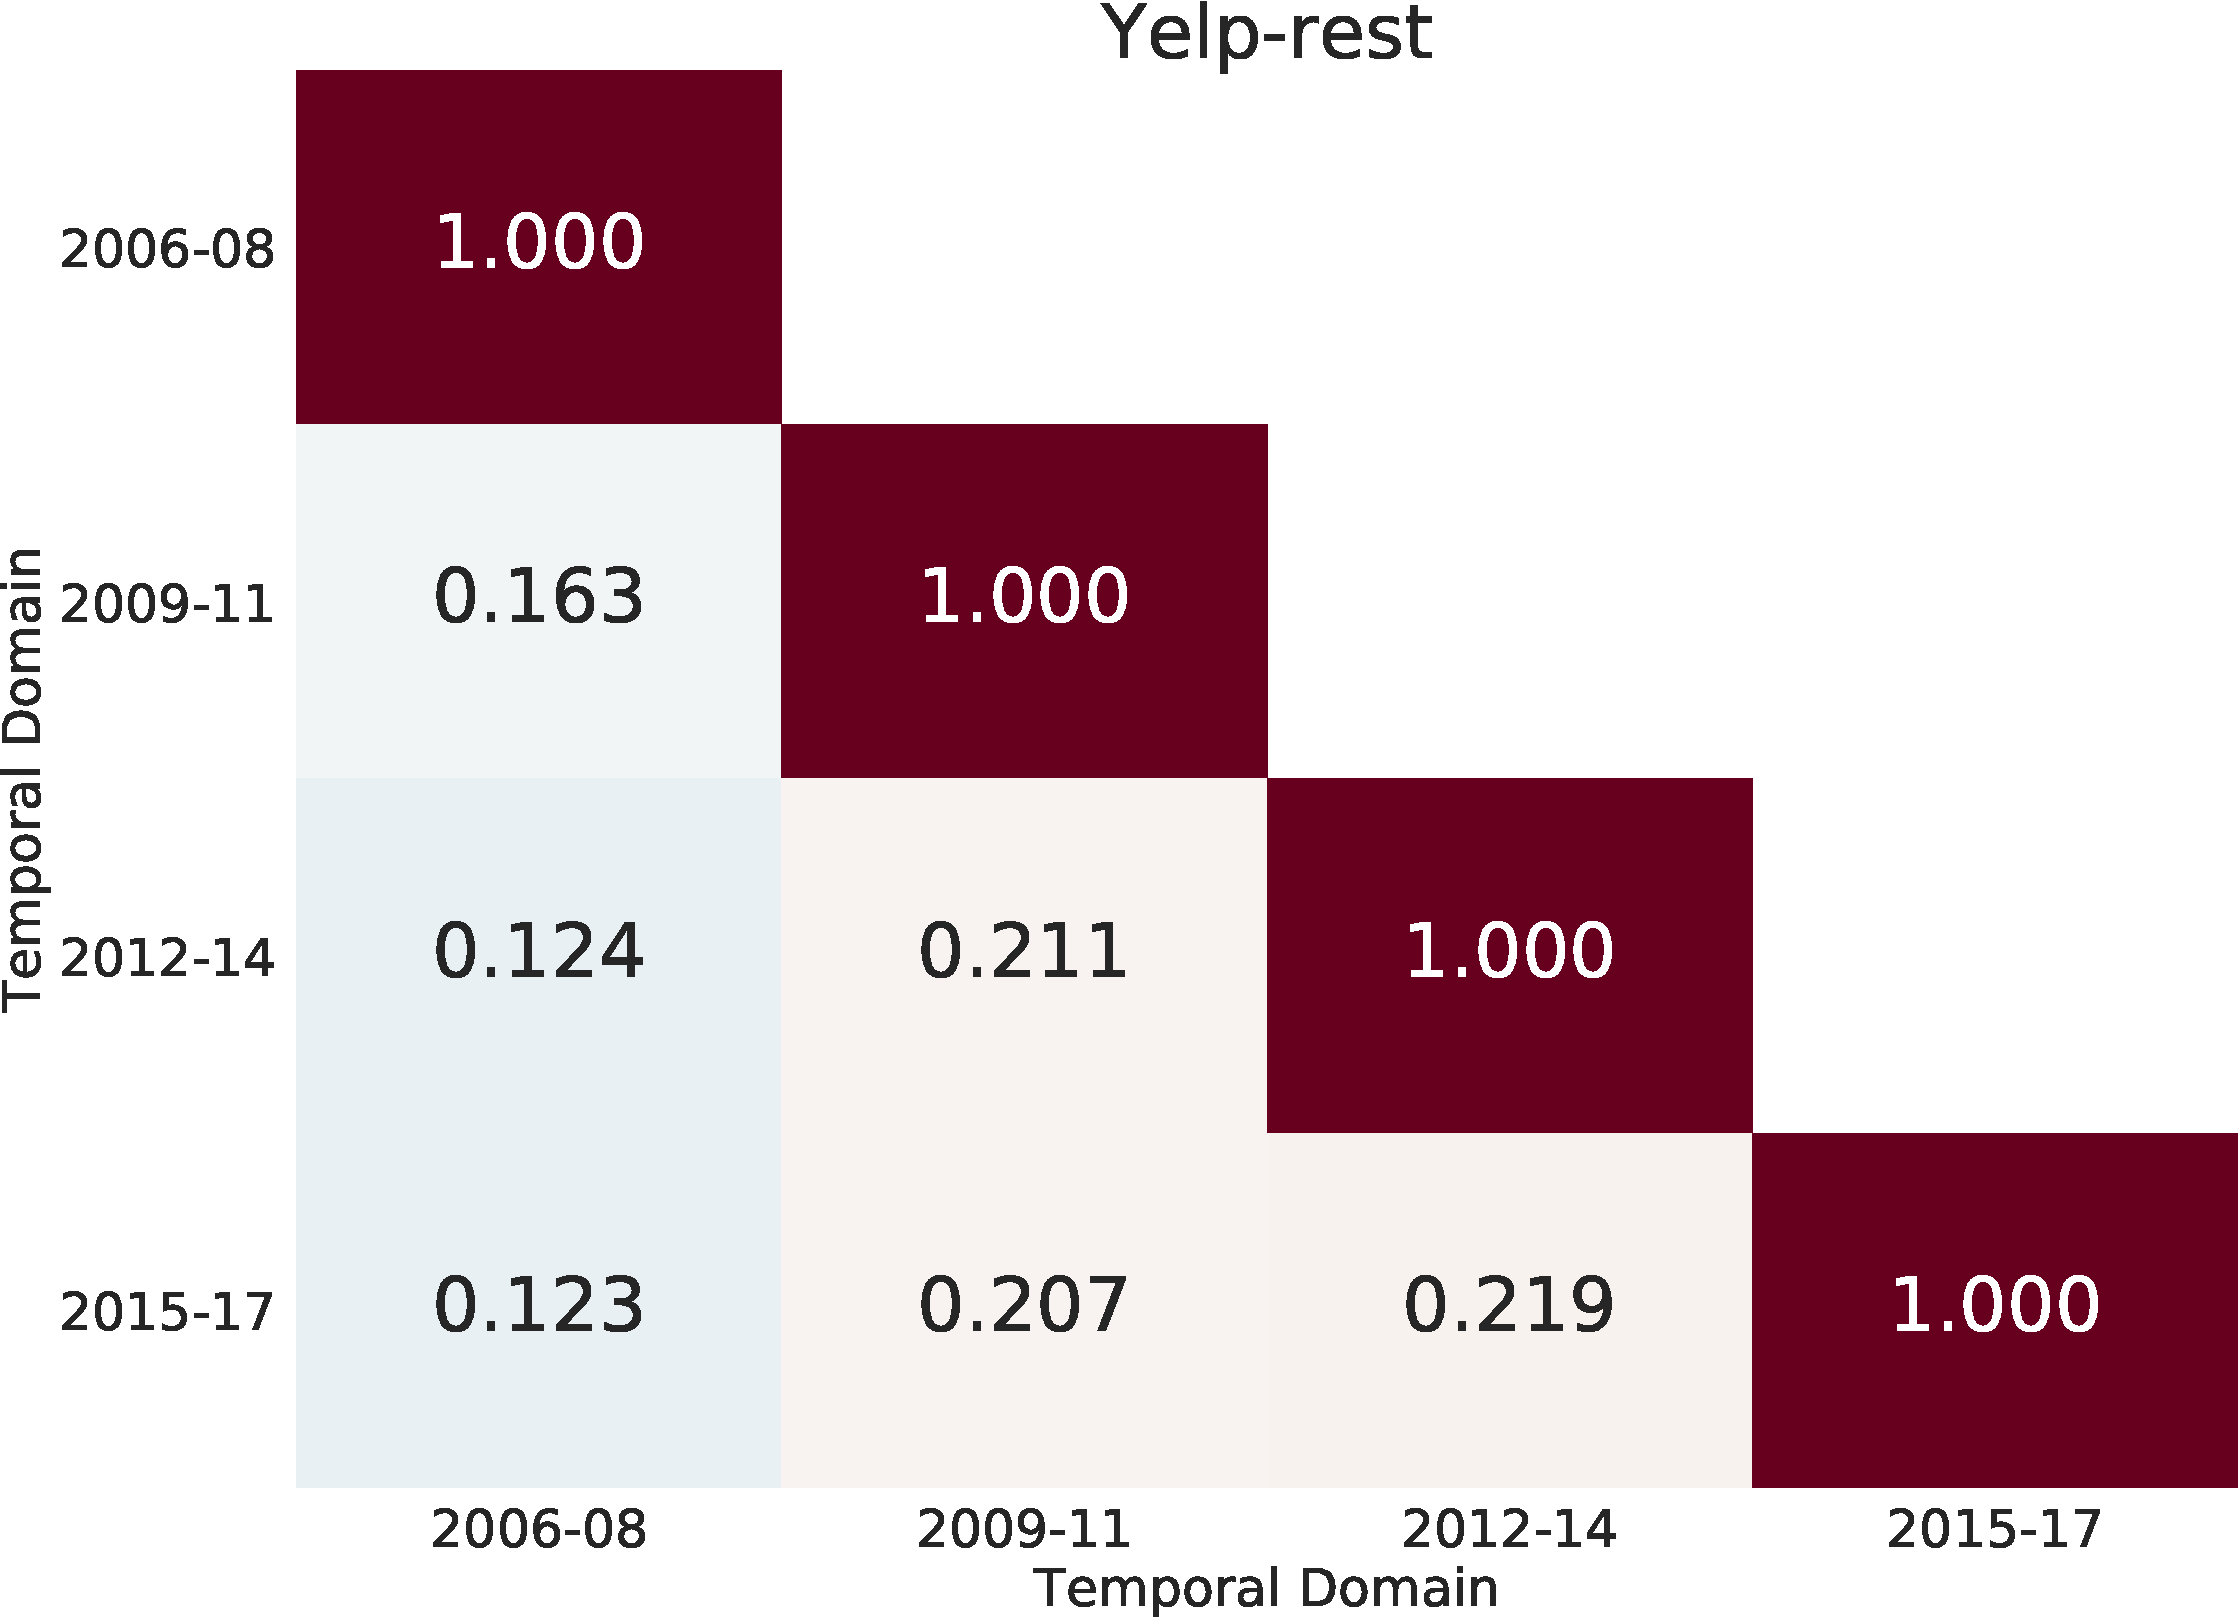
\includegraphics[width=0.31\textwidth]{images/chapter3/ctt_shift/yelp_rest.pdf}
\caption{Context overlaps between every two temporal domains. A value of 0 indicates the contexts of top features between two temporal domains have nothing in common, while values away from 0 mean the contexts share more similarities.}
\label{chap3:fig:ctt}
\end{figure}

Popular word representations for classification train word embeddings using the \textit{context} of each word (a window around the word, e.g., in skip-gram or continuous bag of words methods)~\cite{mikolov2013distributed, bojanowski2017enriching}.
Therefore, we seek to understand how semantic contexts of words shift across time, in addition to the words themselves. 
If we observe a significant context shift, this could lead to inconsistent semantic representations across time.

In the case of context shift, we extract the same unigram features as in the previous section and define word contexts by simulating the word embedding training process via contextual windows. We set a window size of five words and record the words that occur within the context windows. Following the previous section but using the set of words that appear in the context windows, we then calculate the intersection overlap between each pair of time domains.  

We show the overlap in the Figure~\ref{chap3:fig:ctt}.
The overlap percentages range from 0.070 to 0.378. We also observe that temporally closer domains share higher percentages of contextual words. The pattern aligns with our observations in the Section~\ref{chap3:subsec:wusage}. 
Since word embeddings rely heavily on contextual information~\cite{mikolov2013distributed}, our observations that contexts have little overlap across different time intervals therefore suggest it will be important to account for temporality in word embeddings.


\subsection{Analysis 3: Topic Shift}
\label{chap3:subsec:topic}

\begin{figure*}
\centering
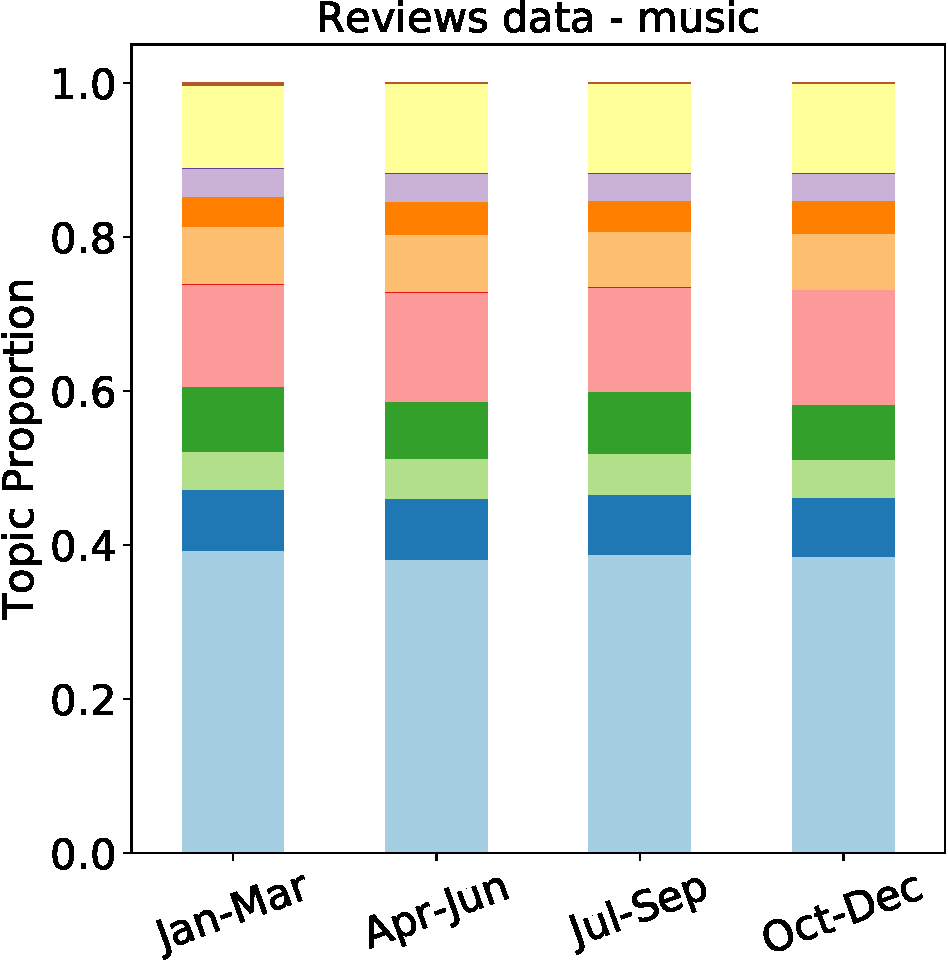
\includegraphics[width=0.23\textwidth]{images/chapter3/acl2018/topic_amazon_month.pdf}
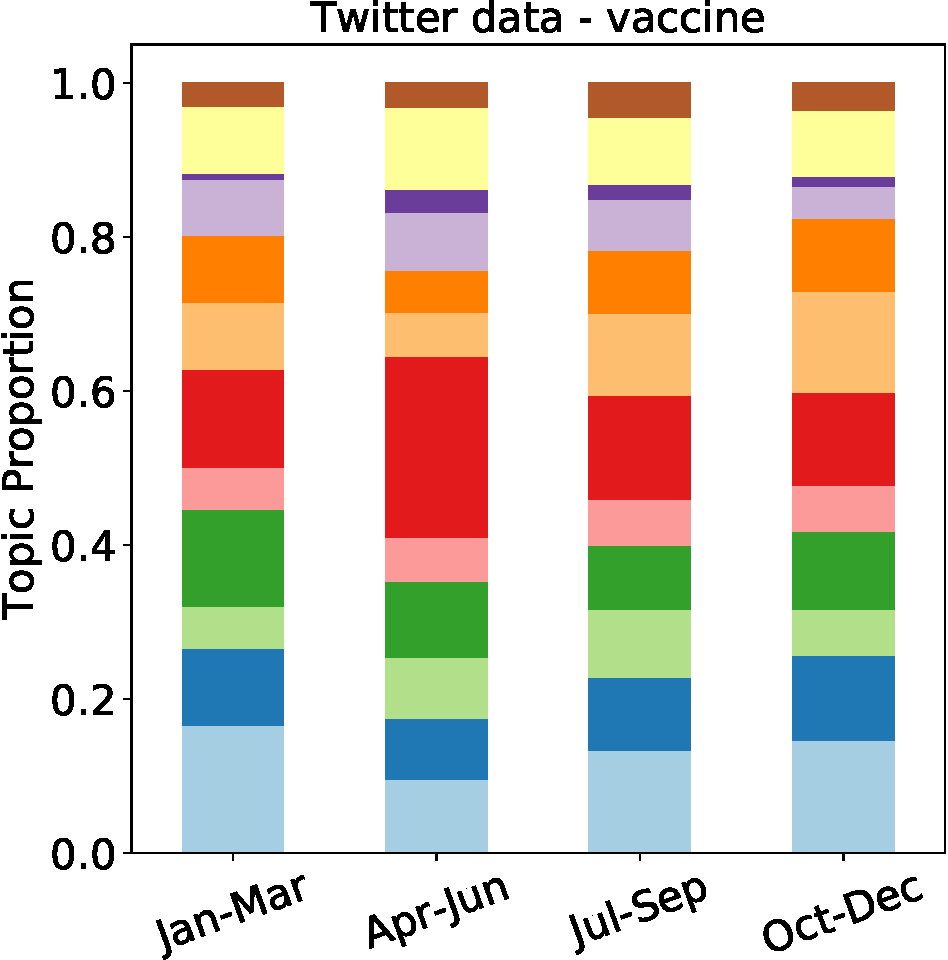
\includegraphics[width=0.23\textwidth]{images/chapter3/acl2018/topic_vaccine_month.pdf} 
\quad
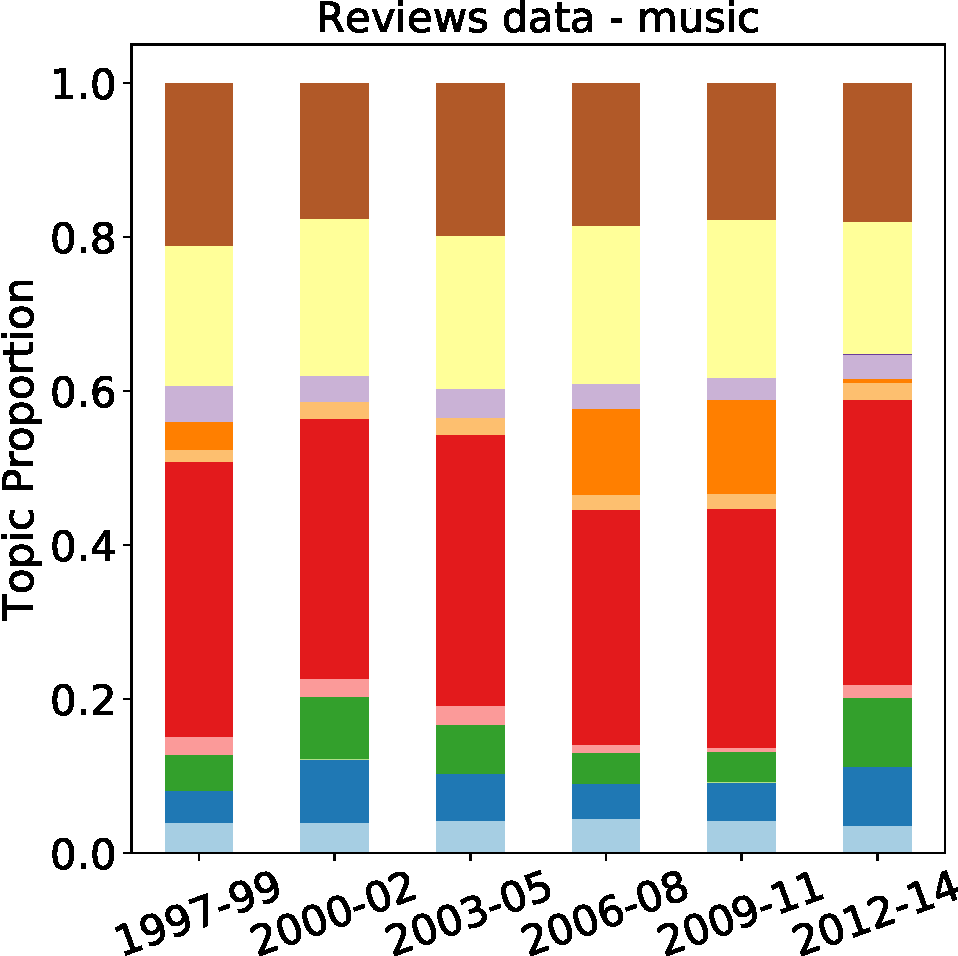
\includegraphics[width=0.23\textwidth]{images/chapter3/acl2018/topic_amazon_year.pdf}
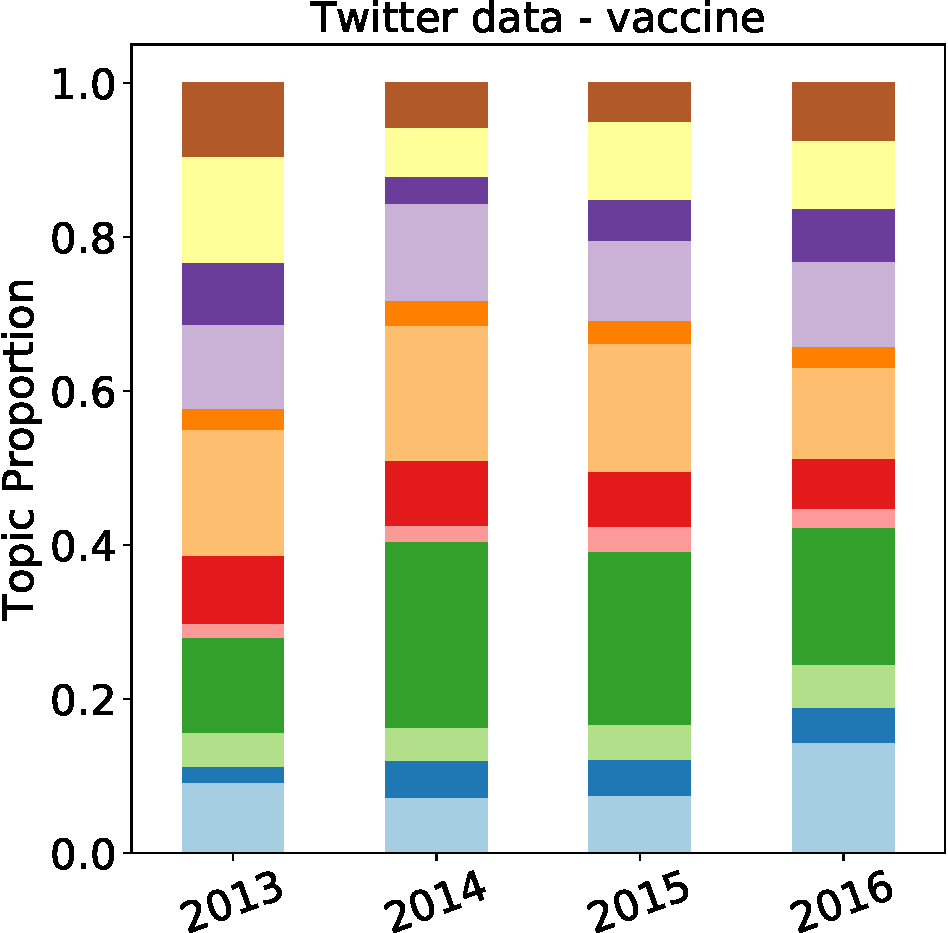
\includegraphics[width=0.23\textwidth]{images/chapter3/acl2018/topic_vaccine_year.pdf}
\caption{\label{chap3:fig:topic} Topic distributions in each time of year (left) and each span of years (right). Topic models are trained independently in the seasonal vs. non-seasonal settings and are not aligned. The music and vaccine refer to Amazon and Twitter datasets respectively.}
\end{figure*}

Finally, to understand why performance varies, we also qualitatively examined how the distribution of content changes across time intervals.
To measure the distribution of content, we trained a topic model with 20 topics using \texttt{Gensim}~\cite{rehurek2010software} with default parameters.
We associated each document with one topic (the most probable topic in the document), and then calculated the proportion of each topic within a time period as the proportion of documents in that time period assigned to that topic.
We can then visualize the extent to which the distribution of 20 topics varies by time.

Figure~\ref{chap3:fig:topic} (left) shows the distribution of topics in each seasonal interval for two corpora: Amazon music reviews and Twitter.
We observe very little variation in the topic distribution across seasons while some changes across non-seasonal intervals in the Amazon corpus, but more variations in the Twitter corpus, which may explain the large performance differences when testing on held-out seasons in the Twitter data as compared to the Amazon corpus.


\subsection{Analysis 4: Impacts on Document Classifiers}

\begin{figure*}[tb!]
\centering
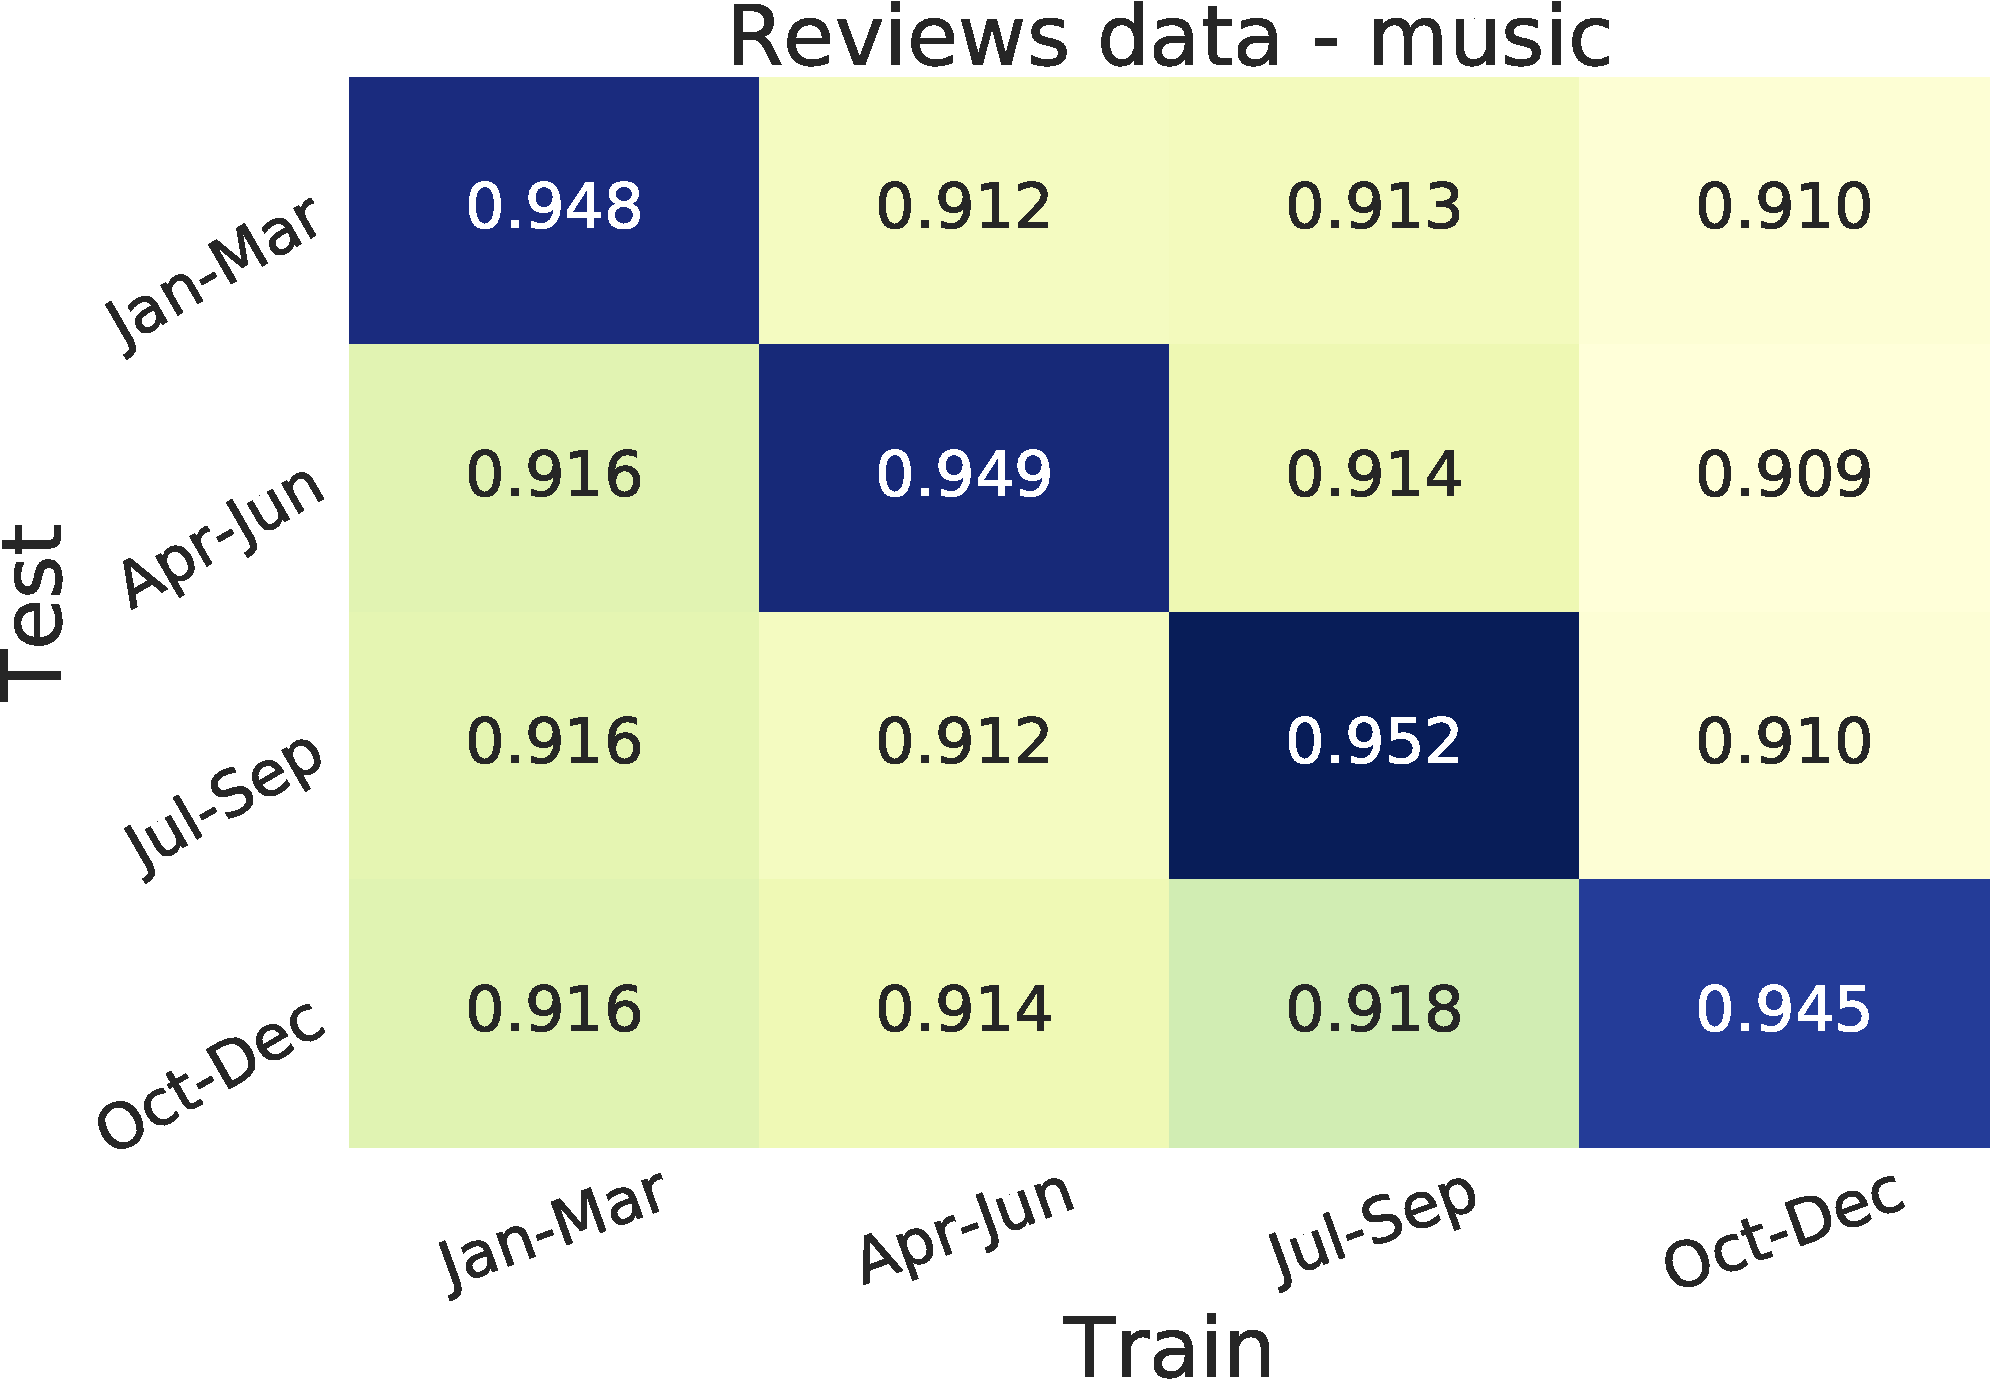
\includegraphics[width=0.244\textwidth]{images/chapter3/acl2018/month_amazon}
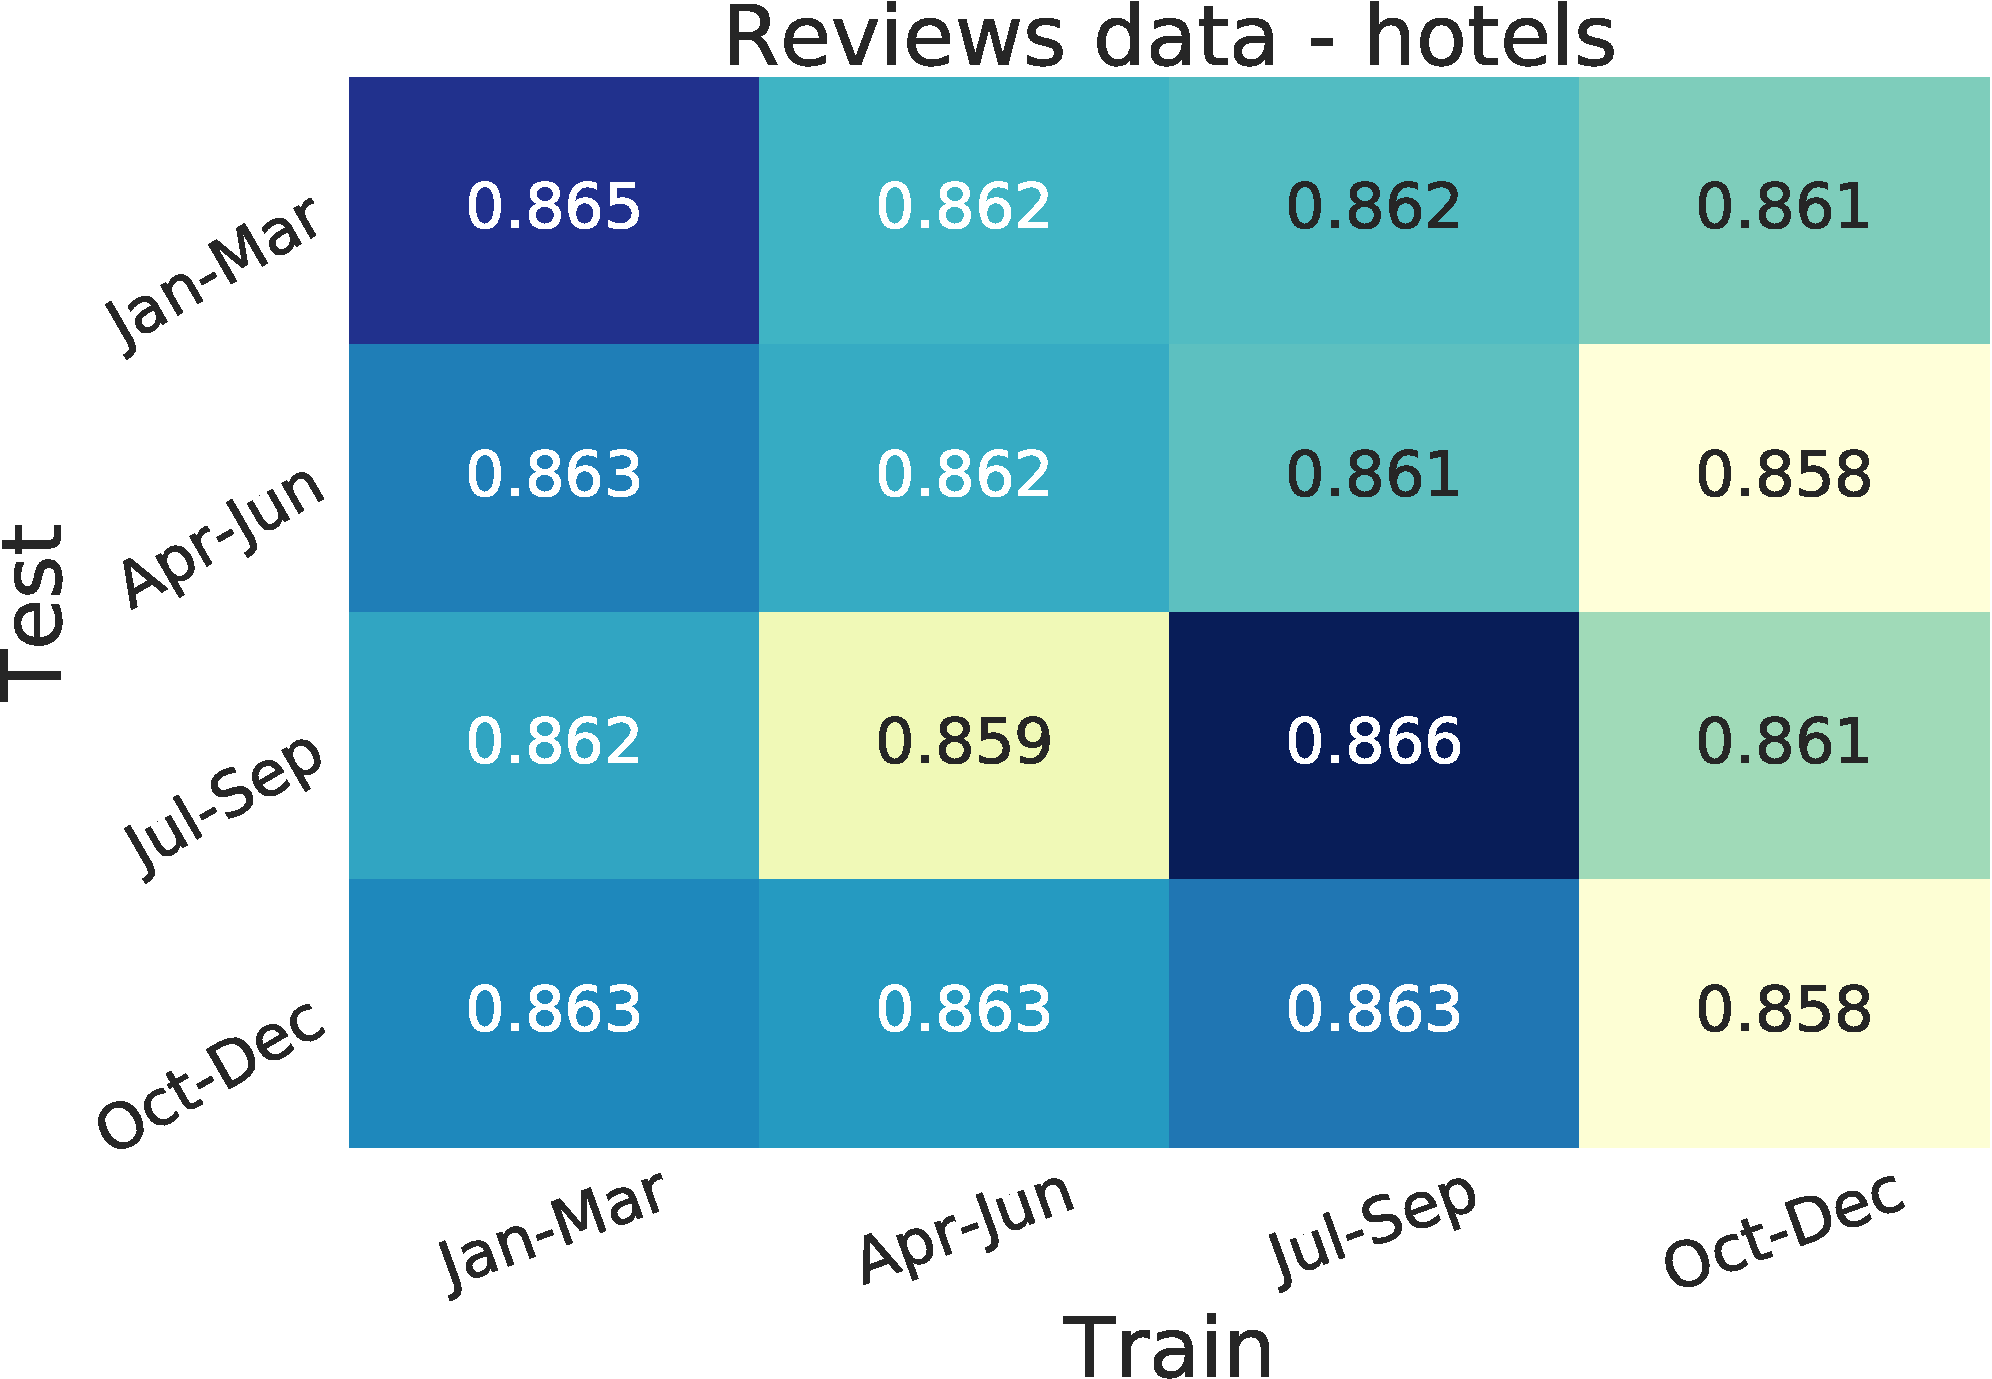
\includegraphics[width=0.244\textwidth]{images/chapter3/acl2018/month_hotel}
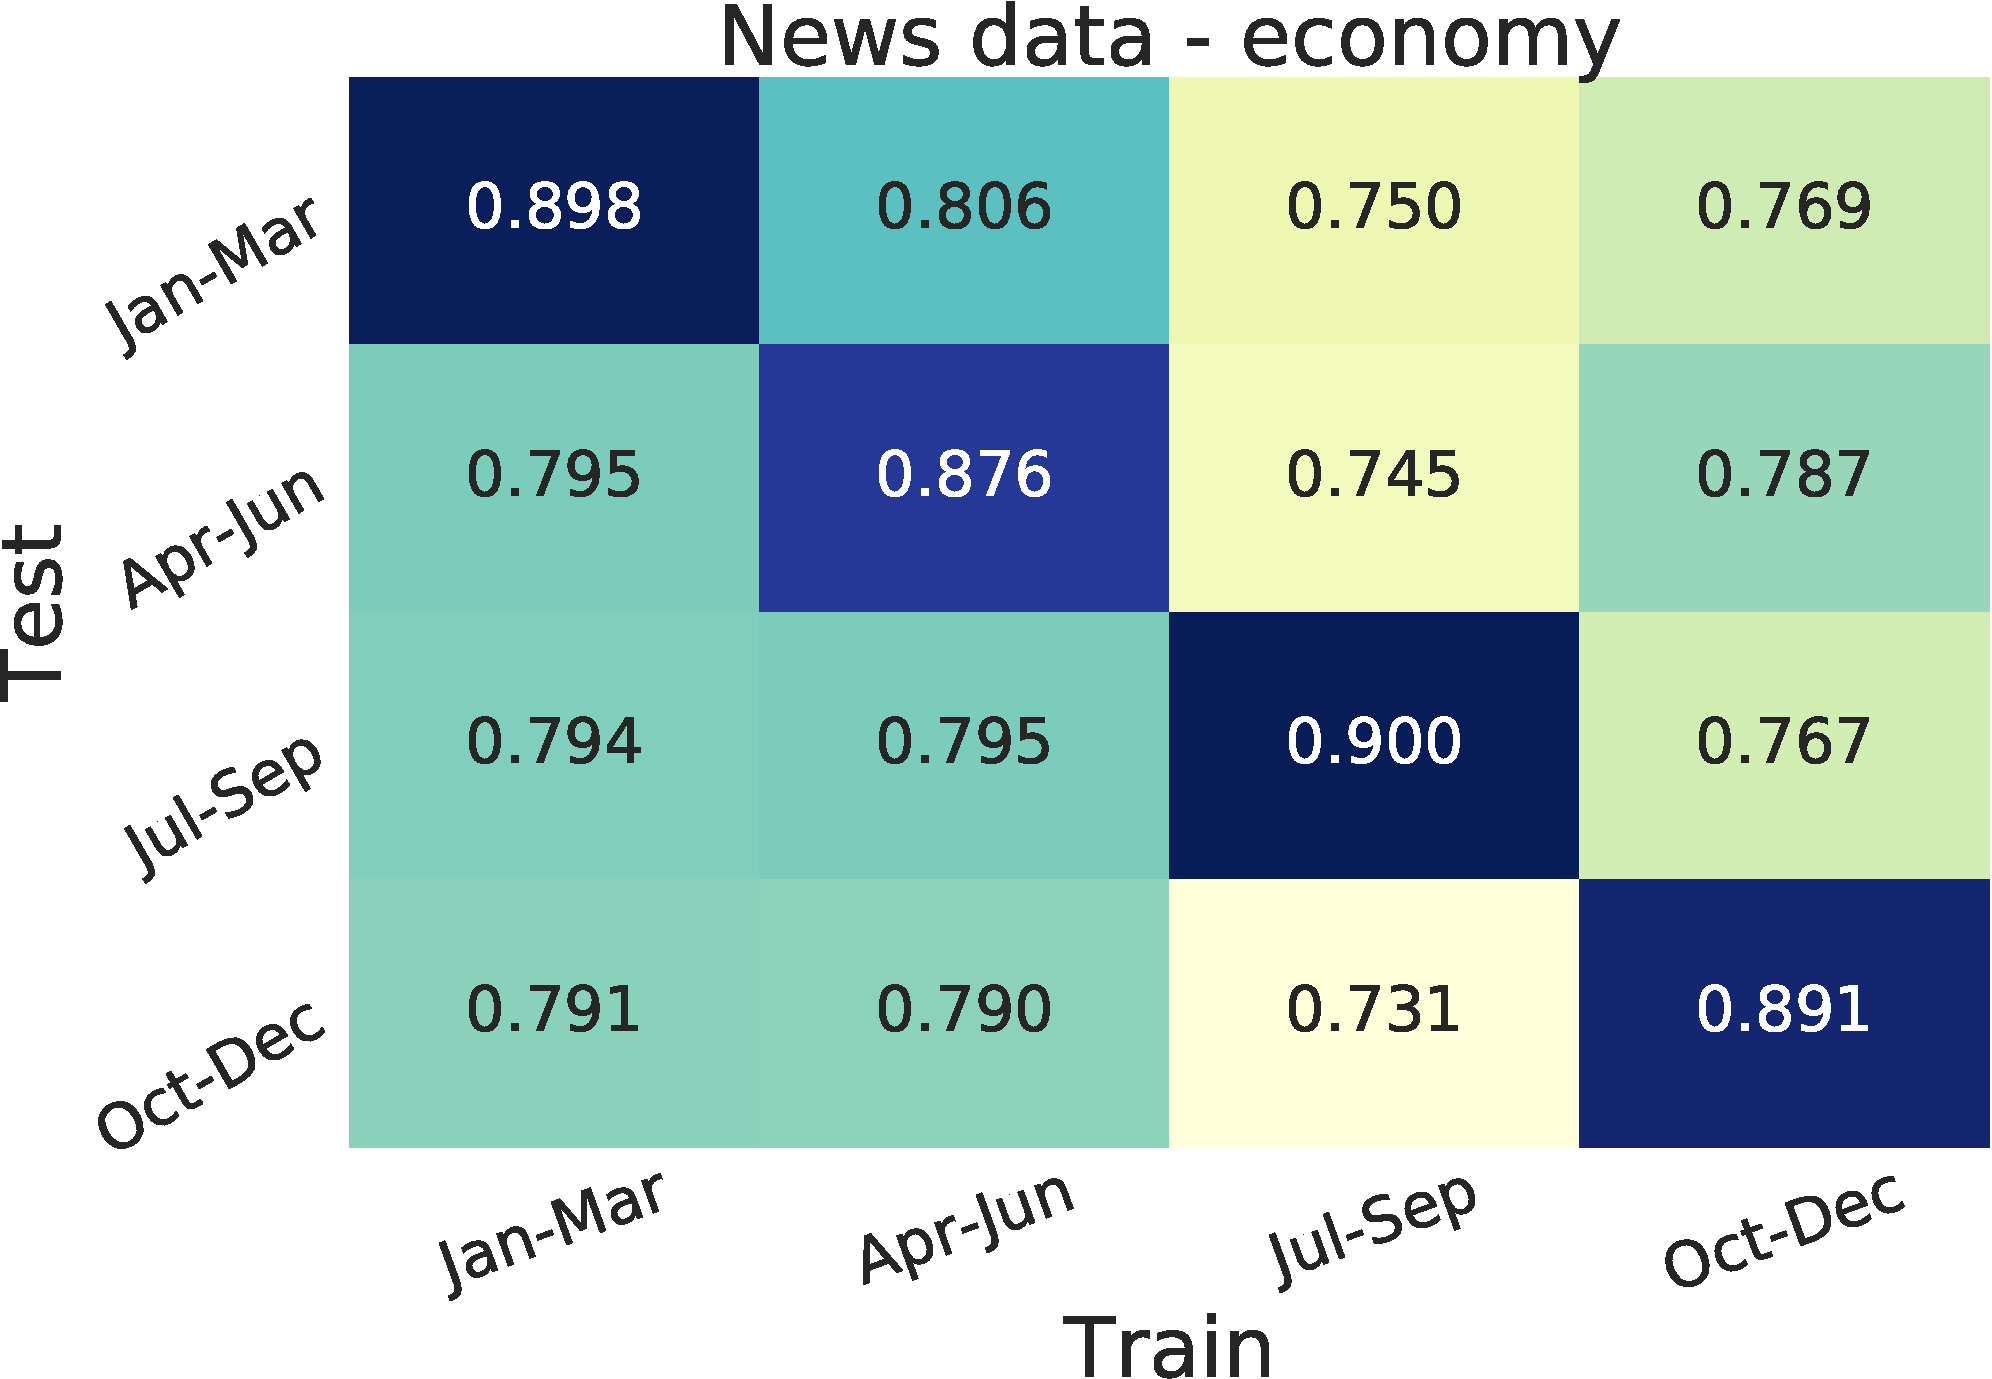
\includegraphics[width=0.244\textwidth]{images/chapter3/acl2018/month_economy}
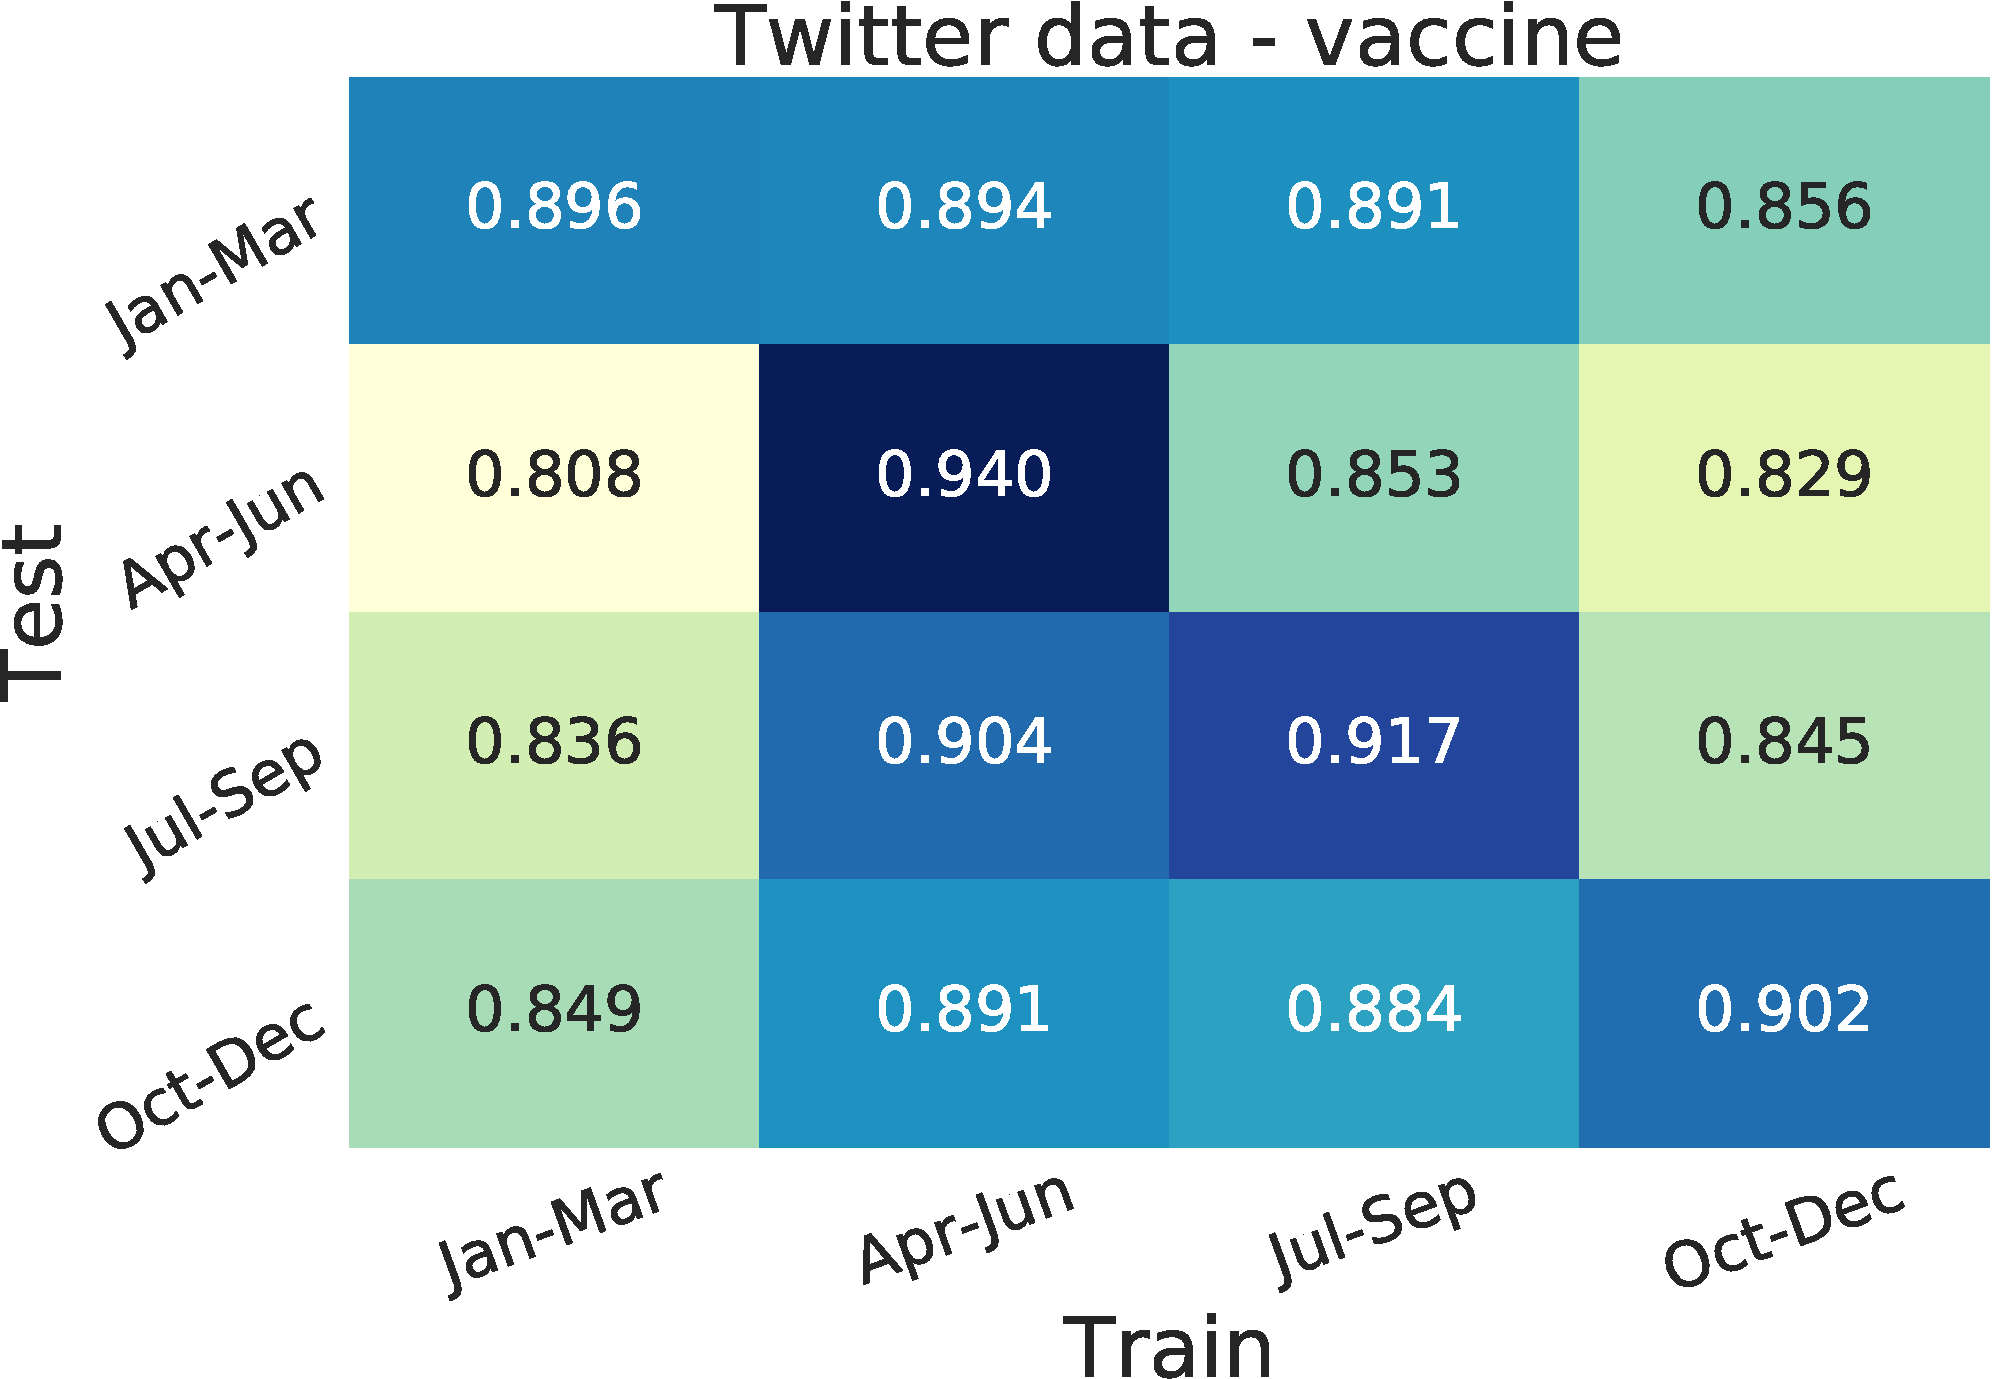
\includegraphics[width=0.244\textwidth]{images/chapter3/acl2018/month_vaccine} \\

\vspace{2ex}

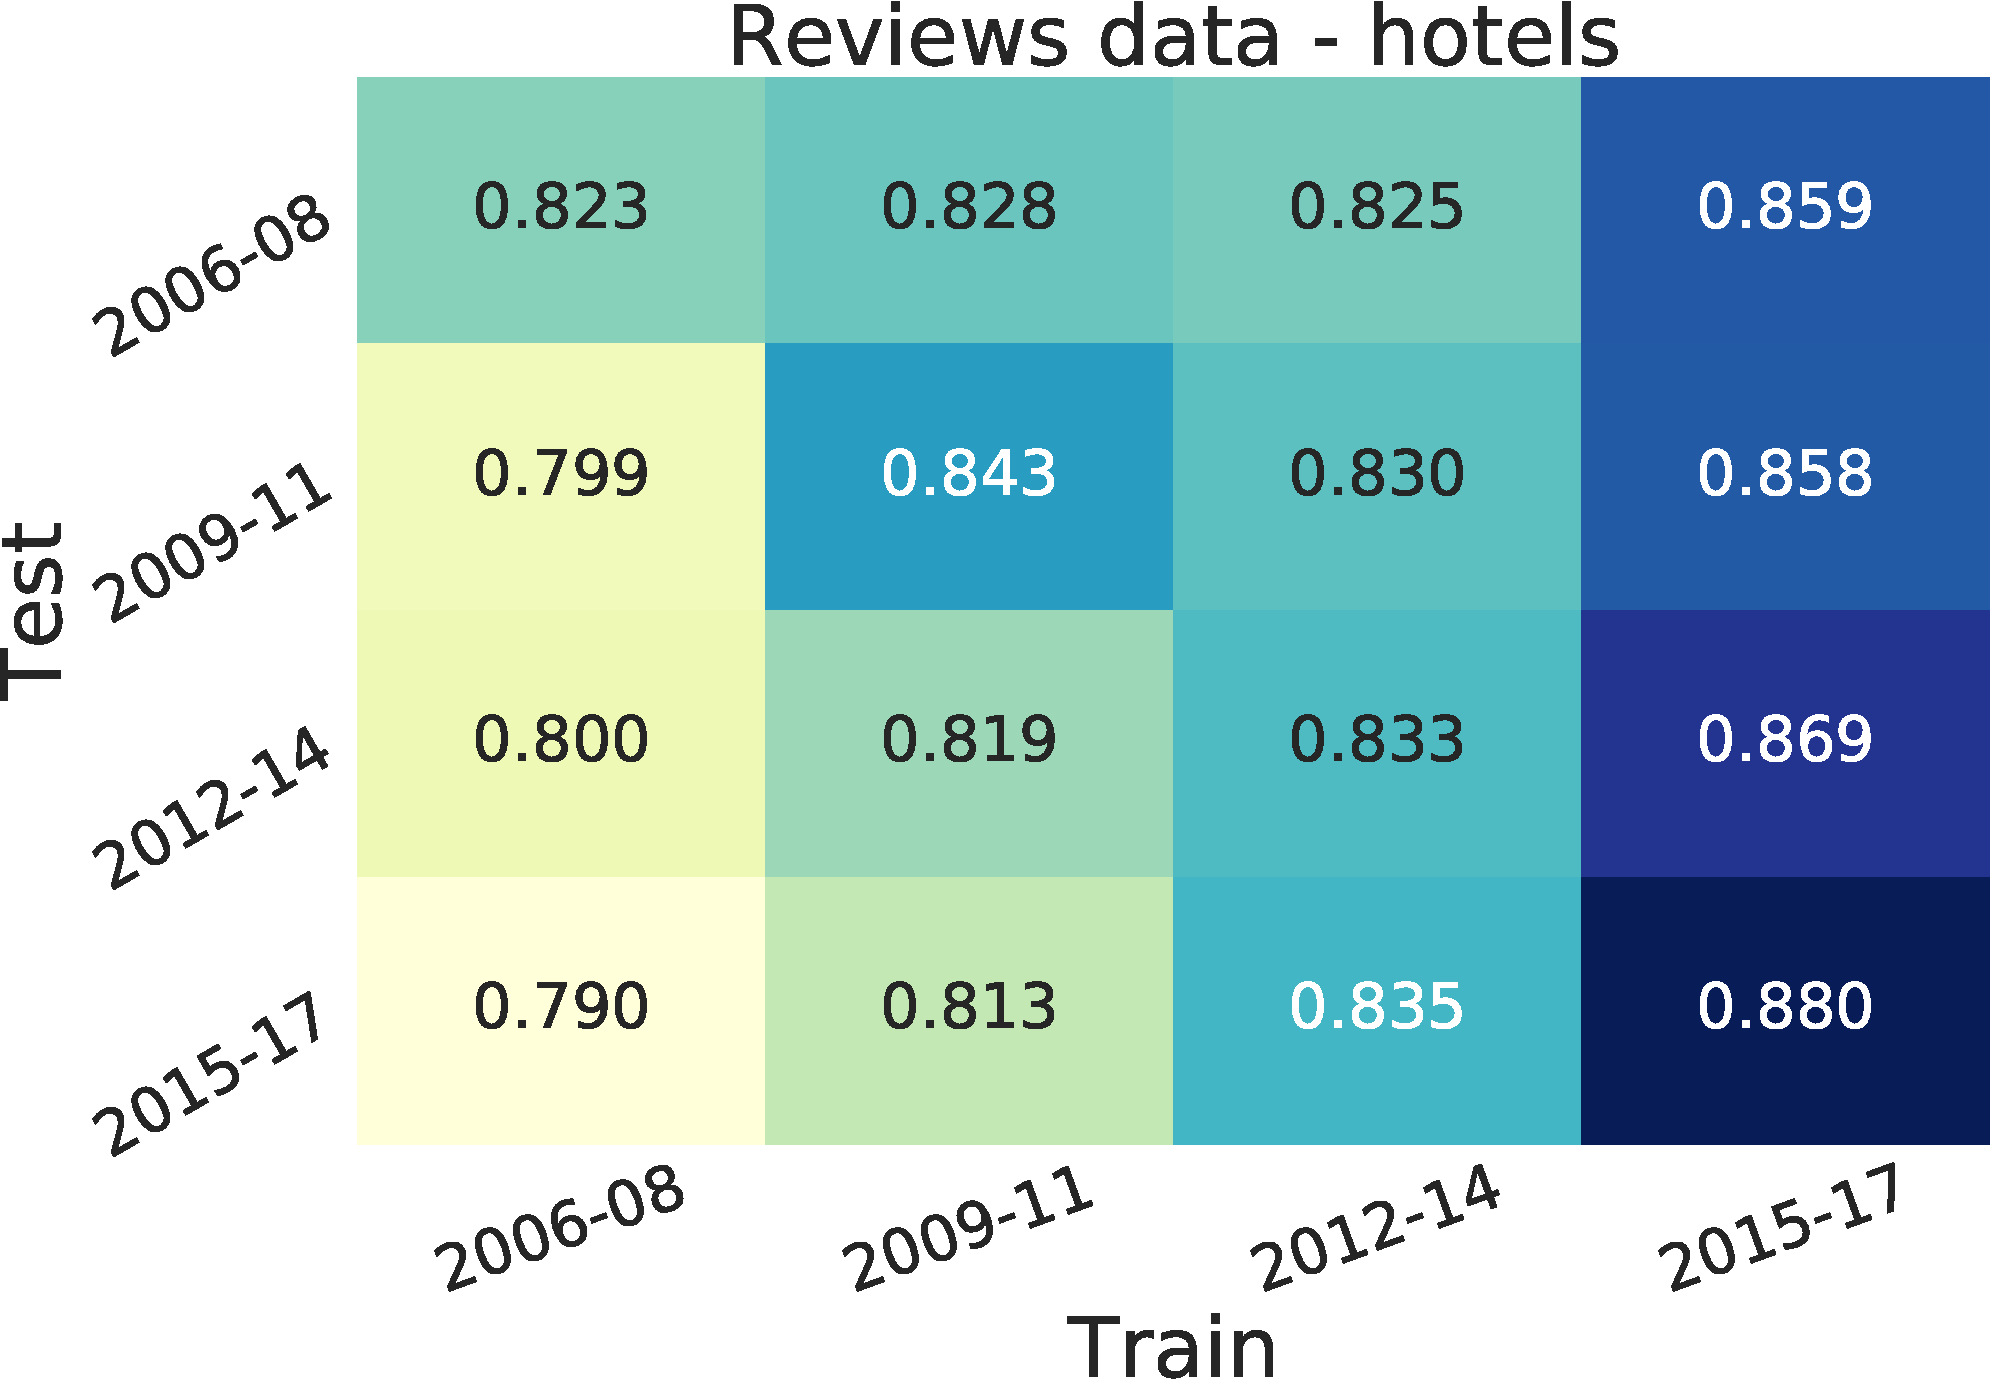
\includegraphics[width=0.244\textwidth]{images/chapter3/acl2018/year_hotel}
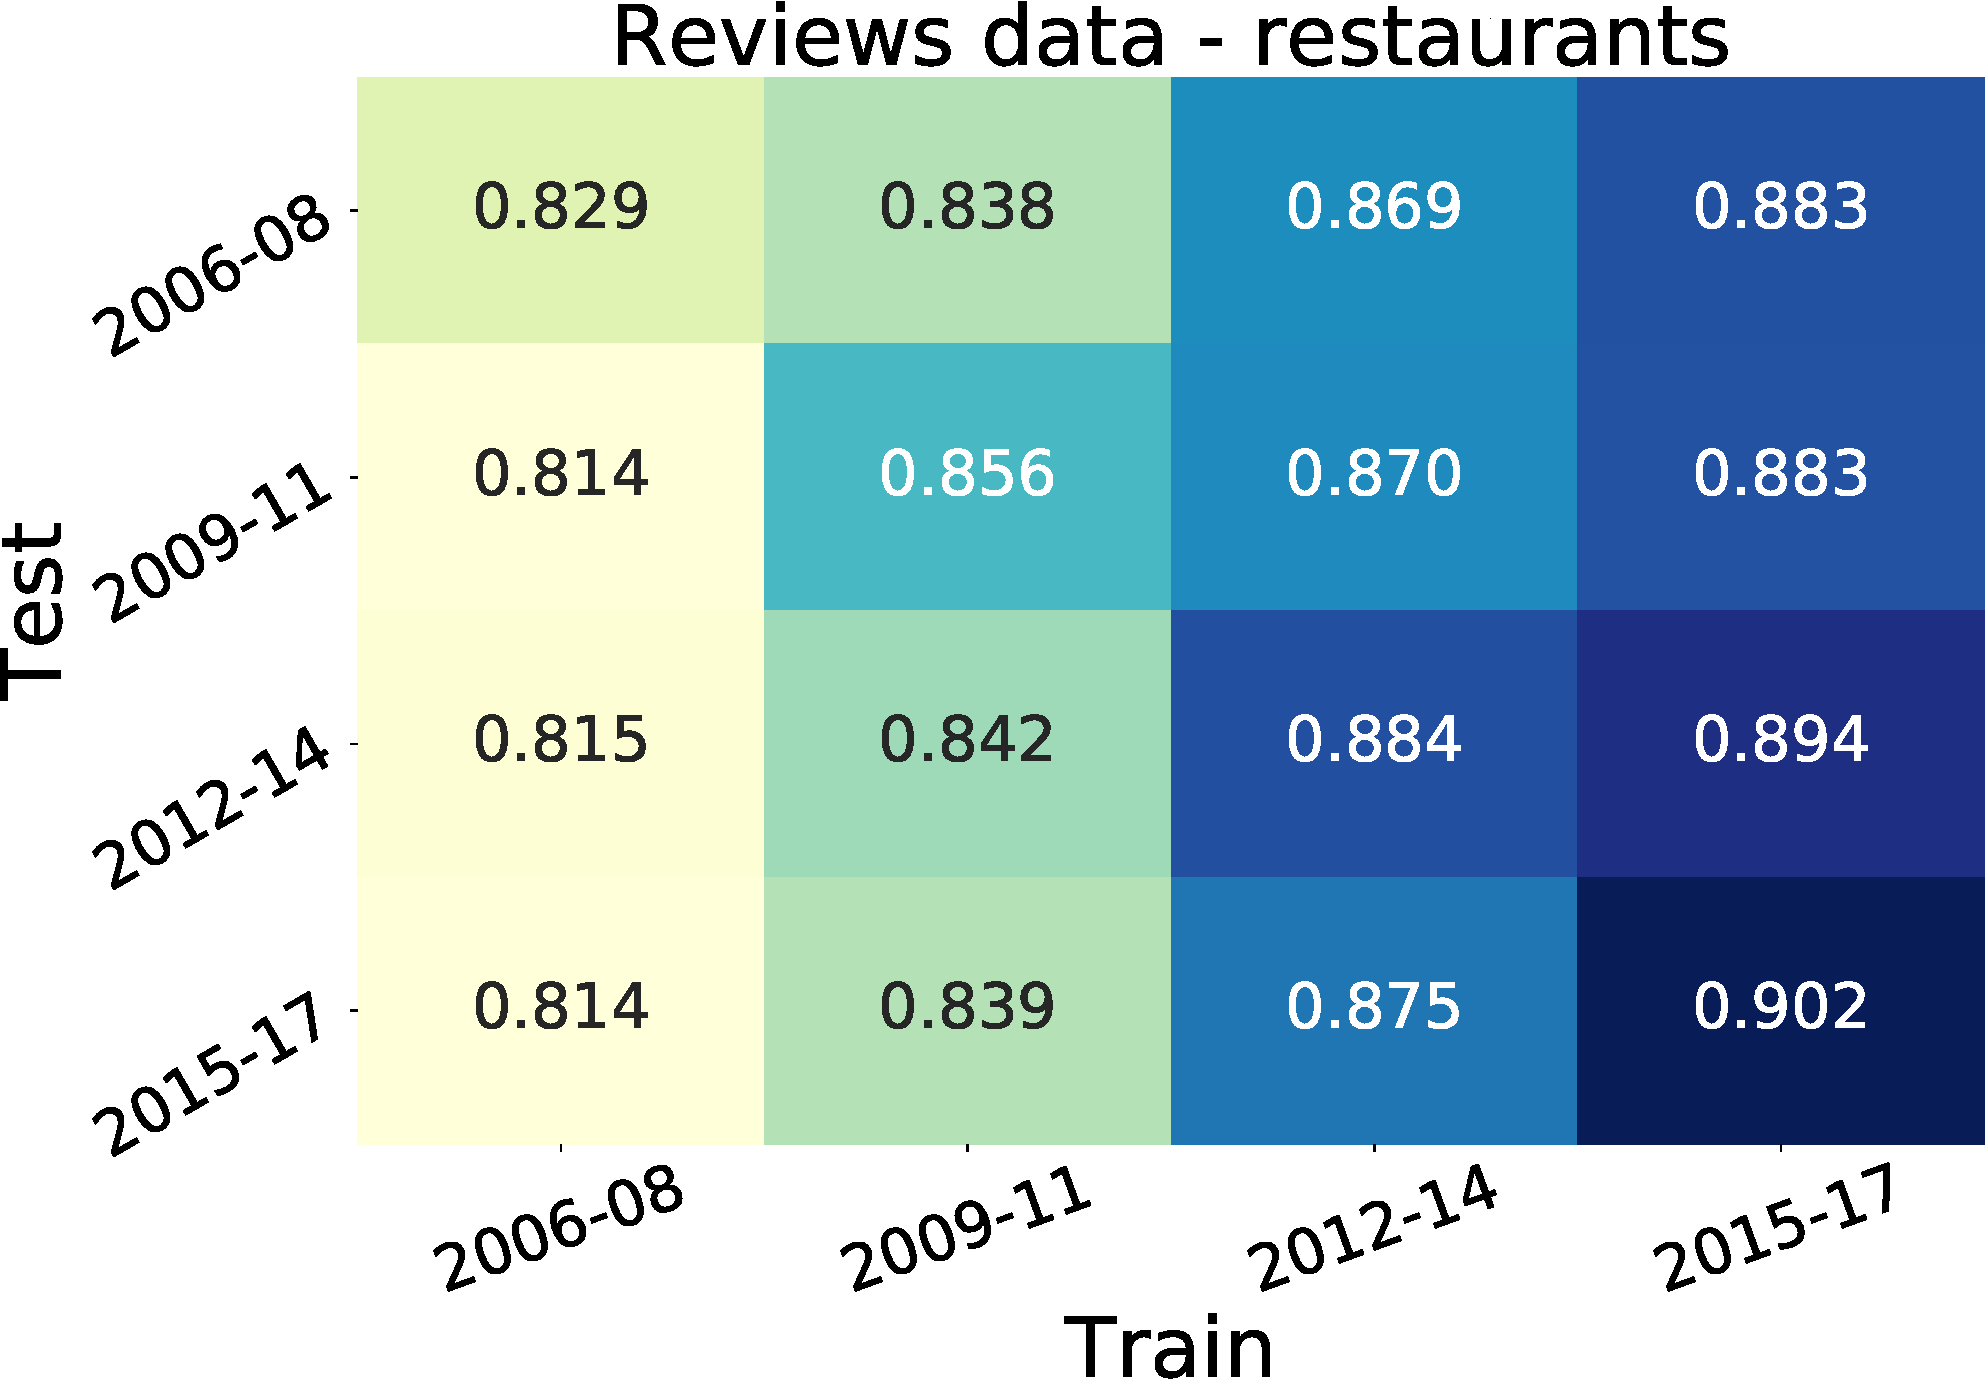
\includegraphics[width=0.244\textwidth]{images/chapter3/acl2018/year_rest}
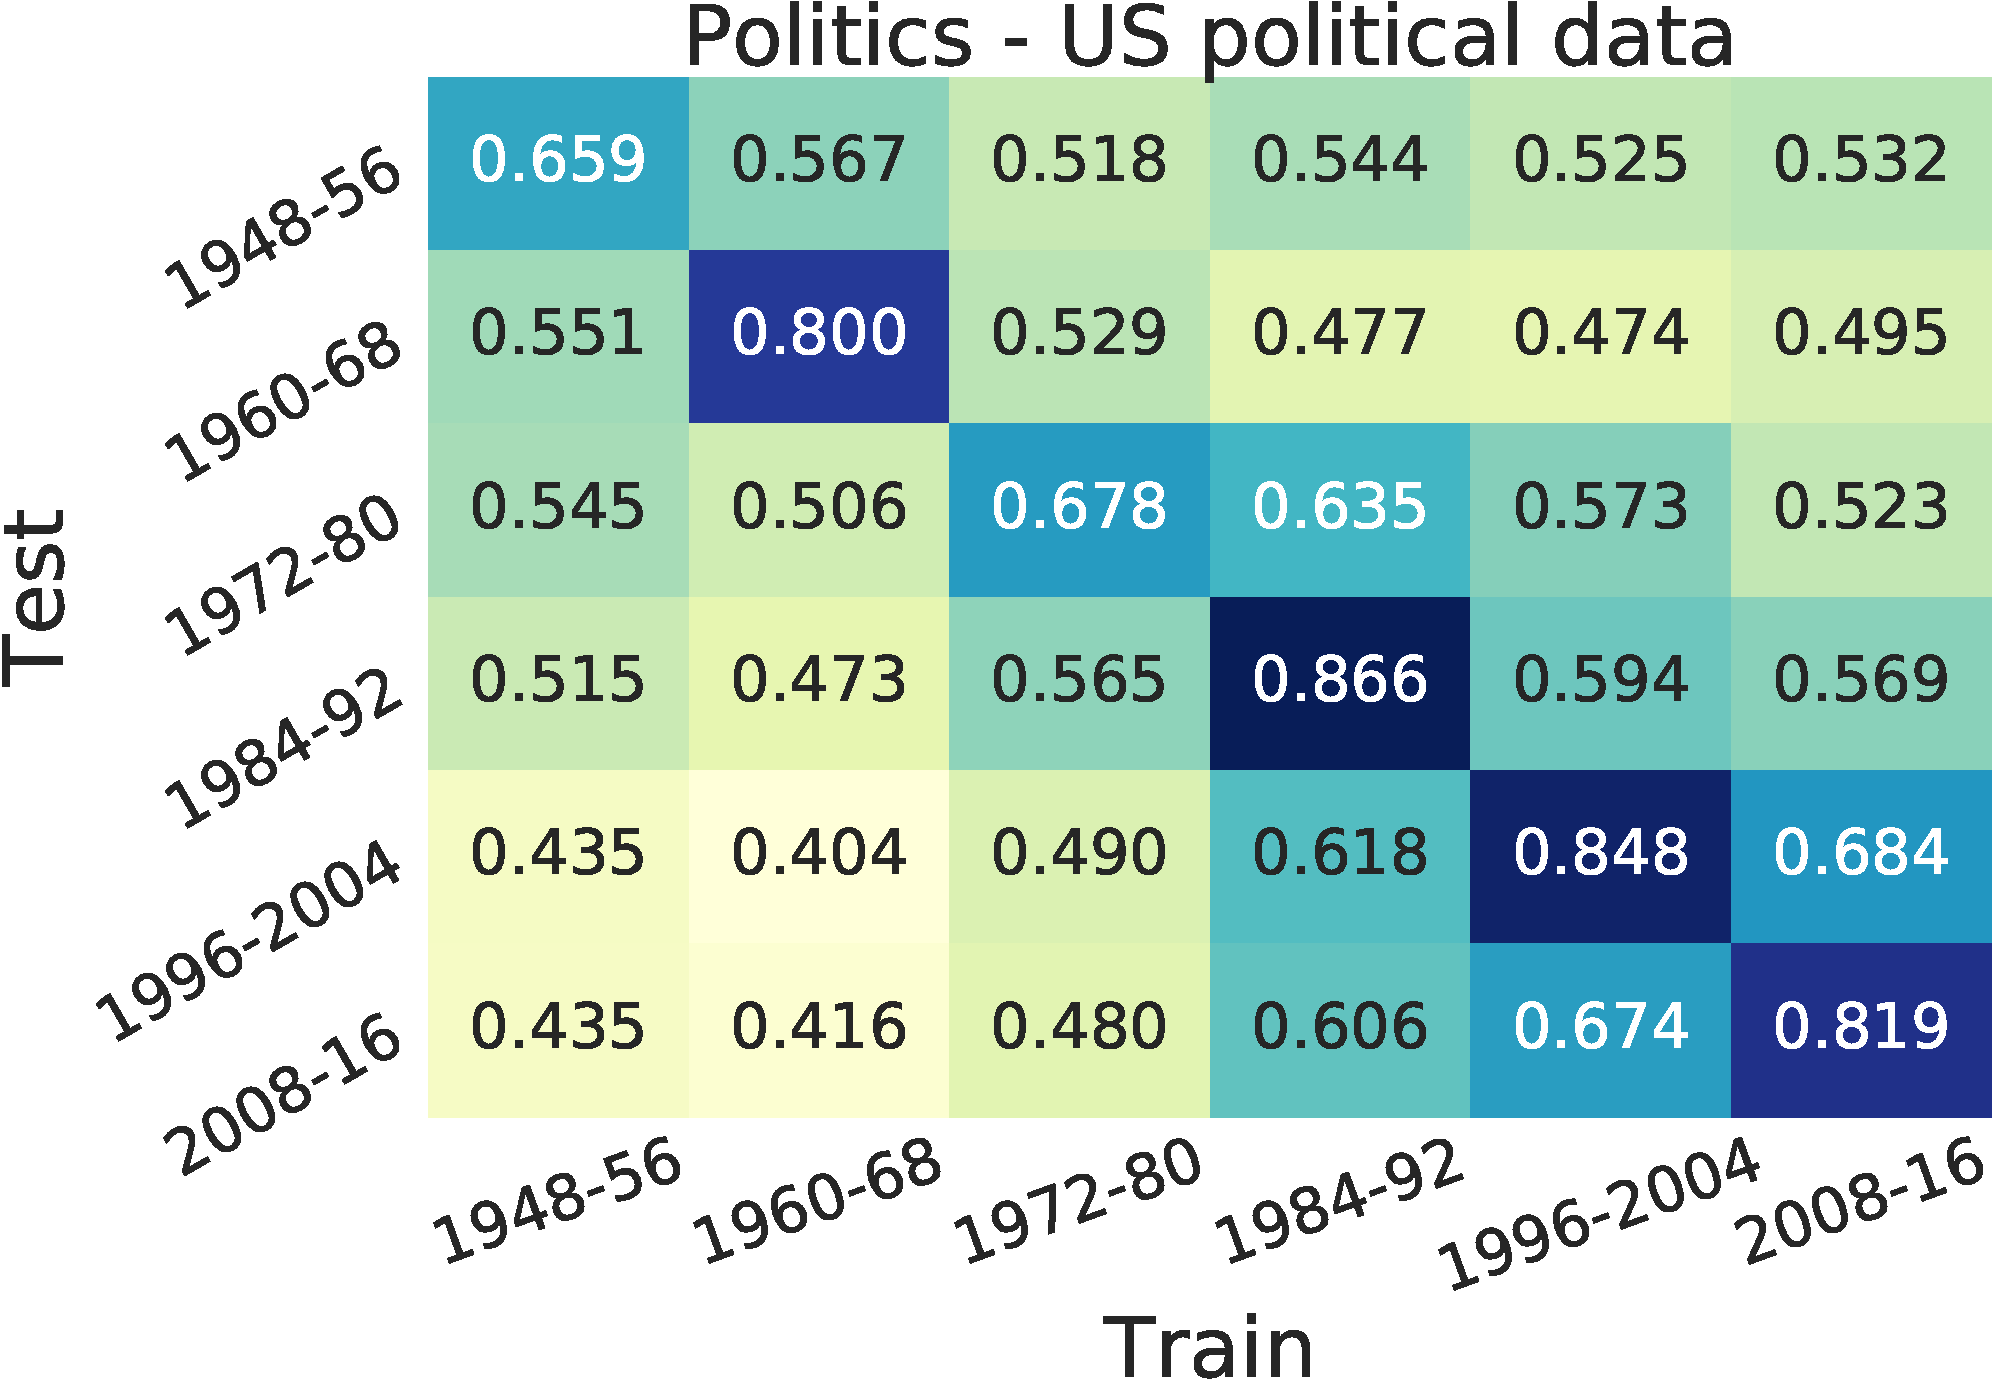
\includegraphics[width=0.244\textwidth]{images/chapter3/acl2018/year_parties}
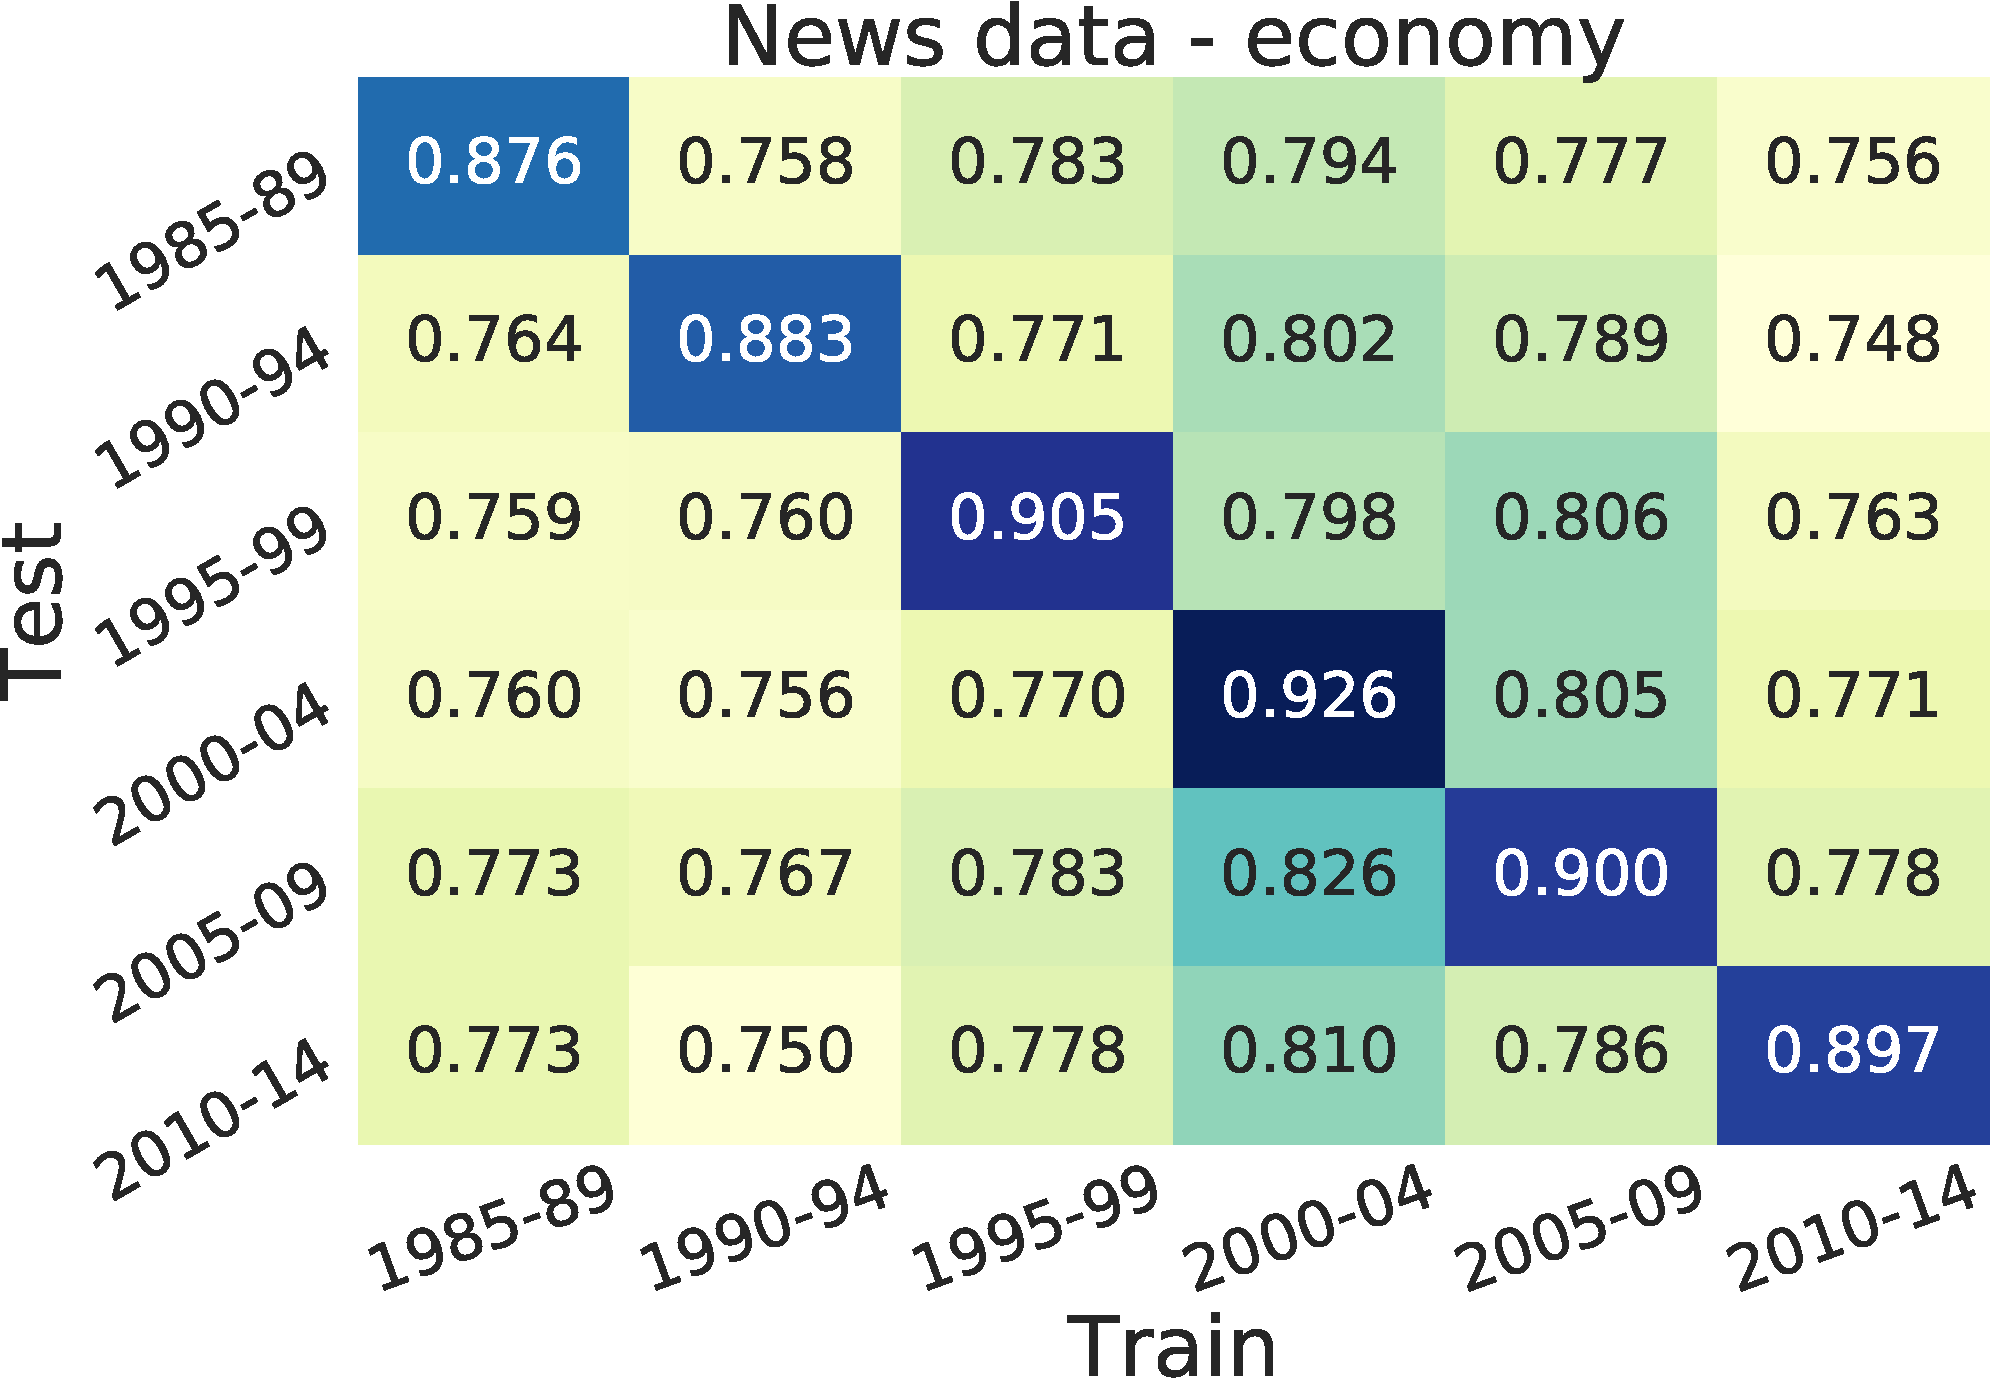
\includegraphics[width=0.244\textwidth]{images/chapter3/acl2018/year_economy}
\caption{\label{chap3:fig:time} Document classification performance when training and testing on different times of year (top) and different years (bottom). The datasets come from Amazon music reviews, Yelp hotel reviews, Economical news reports and Twitter. Darker indicate better classification performance.}
\end{figure*}

The Section \ref{chap3:subsec:wusage}, \ref{chap3:subsec:ctt_shift} and \ref{chap3:subsec:topic} show document features from word, context and topic have shifted overtime. In this section, we investigate how the shifts impact on the performance of document classifiers.

We first conduct an analysis of how classifier performance depends on the time intervals in which it is trained and applied.
For each corpus, we train the classifier on each time interval and test on each time interval.
To keep same labeling format, the reviews with neutral scores were removed.
We downsampled the training data within each time interval to match the number of documents in the smallest interval, so that differences in performance are not due to the size of the training data.

In all experiments, we train a classifier on a partition of 80\% of the documents in the time interval, and repeat this five times on different partitions, averaging the five F1 scores to produce the final estimate. When training and testing on the same interval, we test on the held-out 20\% of documents in that interval (standard cross-validation).
When testing on different time intervals, we test on all documents, since they are all held-out from the training interval; however, we still train on five subsets of 80\% of documents, so that the training data is identical across all experiments.

The Figure~\ref{chap3:fig:time} can demonstrate that the temporal variations directly impact on the performance of document classifiers: 
\begin{itemize}
    \item Classifiers perform best when applied to the same time interval they were trained, and performance diminishes when applied to other time intervals;
    \item Classifiers generally perform worse on farther time intervals than closer time intervals.
\end{itemize}

\subsubsection{Preprocessing}
%MP: The label details are already described in 2.1.
%
We use NLTK~\cite{bird2004nltk} to tokenize the English corpora and the Jieba Python module~\cite{sun2012jieba} to segment the Chinese data. 
We discard reviews that had fewer than 10 tokens. 
For the Twitter data, we anonymize the data and replace usernames, hyperlinks, and hashtags with ``USER'', ``URL'', ``HASHTAG'' respectively. 
All other text is lowercased.
For the four review datasets (Amazon, Dianping, Yelp restaurant and hotel) we encode the 5-point review score into three categories: reviews scores smaller than 3 were labeled as ``0'', larger than 3 are labeled as ``2'', and labeled as ``1'' if the score is 3. We binarize labels of the newspaper, political and Twitter data. 


\section{Feature Augmentation}
\label{chap3:sec:fa}

We now consider how to improve classifiers when working with datasets that span different time intervals.
We propose to treat this as a {\em domain adaptation} problem.
In domain adaptation, any partition of data that is expected to have a different distribution of features can be treated as a domain \cite{joshi2013s}.
Traditionally, domain adaptation is used to adapt models to a common task across rather different sets of data, e.g., a sentiment classifier for different types of products \cite{blitzer-07}.
Recent work has also applied domain adaptation to adjust for potentially more subtle differences in data, such as adapting for differences in the demographics of authors \cite{volkova2013exploring, lynn2017human}.
We follow the same approach, treating time intervals as domains.

In our experiments, we use the feature augmentation approach of \cite{daume2007frustratingly} to perform domain adaptation. Each feature is duplicated to have a specific version of the feature for every domain, as well as a domain-independent version of the feature. In each instance, the domain-independent feature and the domain-specific feature for that instance's domain have the same feature value, while the value is zeroed out for the domain-specific features for the other domains. This is equivalent to a model where the feature weights are domain specific but share a Gaussian prior across domains \cite{Finkel09}.
This approach is widely used due to its simplicity, and derivatives of this approach have been used in similar work (e.g., \cite{lynn2017human}).
Following~\cite{Finkel09}, we separately adjust the regularization strength for the domain-independent feature weights and the domain-specific feature weights.

\subsection{Experiments}

In this section, we conduct experiments on Amazon, Yelp, Twitter, Political and Economy datasets with both seasonal and non-seasonal spans. 
We convert the review datasets into binary labels by discarding documents with the neutral labels.

\subsubsection{Seasonal Adaptation}

\begin{table}[htp]
\centering
\begin{tabular}{|l|l|l|}
\hline
\bf Data (Seasonal) & \bf Baseline & \bf Adaptation \\
\hline
Amazon (reviews) & .901 & \bf .919 \\
Yelp-hotel (reviews) & .867 & \bf .881 \\
Yelp-rest (reviews) & .874 & \bf .898  \\
Economy (news) & .782 & .782  \\
Twitter (vaccines) & \bf .881 & .880  \\
\hline
\end{tabular}
\caption{\label{chap3:tab:results_seasonal} F1 scores when treating each seasonal time interval as a domain and applying domain adaptation compared to using no adaptation.}
\end{table}

We first examine classification performance on the datasets when grouping the seasonal time intervals (January-March, April-June, July-August, September-December) as domains and applying the feature augmentation approach for domain adaptation. 
As a baseline comparison, we apply the same classifier, but without domain adaptation.

Results are shown in Table~\ref{chap3:tab:results_seasonal}.
We see that applying domain adaptation provides a small boost in three of the datasets, and has no effect on two of the datasets.
If this pattern holds in other corpora, then this suggests that it does not hurt performance to apply domain adaptation across different times of year, and in some cases can lead to a small performance boost.

\subsubsection{Non-seasonal Adaptation}
\label{subsec:nonseasonal}

\begin{table*}[htp]
\centering
\begin{tabular}{|l|l|l|l|}
\hline
\bf Data (Non-seasonal) & \bf Baseline & \bf Adaptation & \bf Adapt.+seasons \\
\hline
Amazon (reviews) & .895 & \bf .924 & .910 \\
Yelp-hotel (reviews) & .886 & .892 & \bf .920 \\
Yelp-rest (reviews) & .831 & .879 & \bf .889   \\
Economy (news) & .763 & .780 & \bf .859 \\
Politics (platforms) & .661 & \bf .665 & n/a \\
Twitter (vaccines) & .910 & .903 & \bf .920 \\
\hline
\end{tabular}
\caption{\label{chap3:tab:results_nonseasonal_future} F1 scores when testing on the final time interval after training on all previous intervals.}
\end{table*}

We now consider the non-seasonal time intervals (spans of years). 
In particular, we consider the scenario when one wants to apply a classifier trained on older data to {\em future} data.
This requires a modification to the domain adaptation approach, because future data includes domains that did not exist in the training data, and thus we cannot learn domain-specific feature weights.
To solve this, we train in the usual way, but when testing on future data, we only include the domain-independent features.
The intuition is that the domain-independent parameters should be applicable to all domains, and so using only these features should lead to better generalizability to new domains.
We test this hypothesis by training the classifiers on all but the last time interval, and testing on the final interval.
For hyperparameter tuning, we used the final time interval of the training data (i.e., the penultimate interval) as the validation set. The intuition is that the penultimate interval is the closest to the test data and thus is expected to be most similar to it.

Results are shown in the first three columns of Table~\ref{chap3:tab:results_nonseasonal_future}.
We see that this approach leads to a small performance boost in all cases except the Twitter dataset. 
This means that this simple feature augmentation approach has the potential to make classifiers more robust to future changes in data.

How to apply the feature augmentation technique to unseen domains is not well understood.
By removing the domain-specific features, as we did here, the prediction model has changed, and so its behavior may be hard to predict.
Nonetheless, this appears to be a successful approach.

\subsubsection{Dual Adaptation}

We also experimented with including the seasonal features when performing non-seasonal adaptation.
In this setting, we train the models with two domain-specific features in addition to the domain-independent features: one for the season, and one for the non-seasonal interval. 
As above, we remove the non-seasonal features at test time; however, we retain the season-specific features in addition to the domain-independent features, as they can be reused in future years.

The results of this approach are shown in the last column of Table~\ref{chap3:tab:results_nonseasonal_future}.
We find that combining seasonal and non-seasonal features together leads to an additional performance gain in most cases.


\section{Diachronic Word Embeddings}
\label{chap3:sec:dwe}

Standard word embeddings ignore temporal language variations in the data. %Ignoring such temporal variations can impact on the stability of word embeddings, and such a ignore can further influence neural document classifiers. 
\textit{Diachronic} word embeddings~\cite{kulkarni2015statistically} 
encode temporality into word embeddings to obtain dynamic representations of words. 
These types of embeddings have been effective in capturing and learning the language usage and semantic shift over time~\cite{kim2014temporal, kulkarni2015statistically, hamilton2016diachronic, bamler2017dynamic, szymanski2017temporal, rudolph2018dynamic, rosenfeld2018deep, yao2018dynamic}. 

To the best of our knowledge, diachronic word embeddings have not been studied in the context of document classification. 
Since our preliminary analyses in the previous section showed that the top features for document classification vary over time, and the contexts used to train those word embeddings also vary over time, 
it would make sense to use word representations that can vary over time.
In this section, we present a new, simple-to-implement method for constructing diachronic embeddings, and then further analyze temporal shifts in corpora using these embeddings.

\subsection{Concatenative Training Approach}

Methods to obtain diachronic word embeddings fall into three main directions: incremental training \cite{kim2014temporal}, alignment transformation \cite{kulkarni2015statistically, hamilton2016diachronic, yao2018dynamic} and continuous time representations \cite{rosenfeld2018deep, rudolph2018dynamic}.

In this work, we propose an alternative approach 
to encoding time into word embeddings.
The idea is inspired by the ``easy'' domain adaptation method \cite{daume2007frustratingly}, which was shown to be successful at modeling different temporal domains \cite{huang2018examining}, and can be implemented by simply modifying the input data without modifying the training process.
In our approach, words in the training data are concatenated with the name of the time interval,
and embeddings are trained using a sub-word sharing framework~\cite{bojanowski2017enriching}. 
The concatenation step allows for the learning of word representations that are specific to each time interval, while the sub-word framework allows for the learning of general, time-independent representations of each word.

Concretely,
we first build domain-specific corpora by adding each document's domain label as a suffix to each word, as shown in  Figure~\ref{chap3:fig:domain}. 
In addition to the domain-specific corpora,
we retain the original corpus as a domain-independent version.
We then train fastText~\cite{bojanowski2017enriching}, a sub-word embedding model, on all of the corpora,
We use 3- to 6-grams characters in this study, to provide  diverse perspectives to encode time and word representations. 
This approach learns diachronic word representations by encoding temporality as part of sub-words into the word embedding. 

\begin{figure}[htp]
\centering
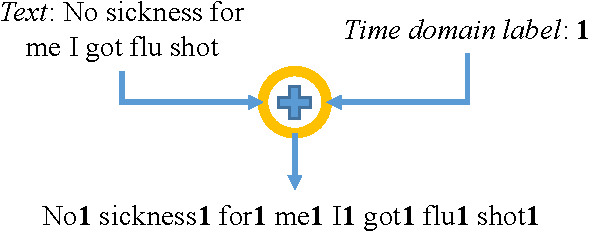
\includegraphics[width=0.55\textwidth]{images/chapter3/domain_doc.pdf}
\caption{The illustration of building domain corpora. We append the document domain label as a suffix to each word in the document.}
\label{chap3:fig:domain}
\end{figure}

FastText learns word embeddings from character n-grams, intended to capture morphological information. As an example example, the word ``where1'' from time domain 1 using character 3-grams would be encoded in fastText as the following seven parts:
\begin{center}
    $<wh, whe, her, ere, re1, e1>, <where1>$
\end{center}

In this way, words with time domain labels can incorporate temporal identities, while the same words with different domain labels will still share close representations because of similar morphological forms. In this way, we encode temporal identity into word representations while still maintaining the connections of the same words across different time domains. 

In contrast to prior approaches on diachronic embeddings, this concatenative sub-word approach does not explicitly model the ordering of time information, and it cannot encode, for example, that domains that are close in time should have more similarities than domains that are farther away in time.
Despite this limitation, we find experimentally that this approach works competitively, while being simpler to implement and faster to train.


\subsection{DWE Evaluation}

In this section, we evaluate effectiveness of our proposed diachronic word embedding modela public test set~\cite{yao2018dynamic}.
The goal is to examine if our proposed DWE model can capture the changing sense of words over time.
In all cases, we keep the dimension of word representations as 200.

\subsubsection{Evaluation Data}
We retrieved available newspaper datasets of New York Times from the previous publication~\cite{yao2018dynamic}.
The dataset contains $99,872$ newspaper articles in 27 years ranging from 1990 to 2016.
We used \textit{RegexpTokenizer} from NLTK~\cite{bird2004nltk} to tokenize the documents that only contain alphabets and numbers.
We then dropped any paragraphs that are less than 5 tokens.
With the time information, we grouped documents in every three years: 1990-1992 (90-92); 1993-1995 (93-95); 1996-1998 (96-98); 1999-2001 (99-01); 2002-2004 (02-04); 2005-2007 (05-07); 2008-2010 (08-10); 2011-2013 (11-13); 2014-16 (14-16). 
We show the details of preprocessed evaluation data in Table~\ref{chap3:tab:dweEvalData}.


\begin{table}[htp]
\centering
\resizebox{\textwidth}{!}{\begin{tabular}{c||cccccccccc}
\begin{tabular}[c]{@{}c@{}}time\\ interval\end{tabular} & 90-92 & 93-95 & 96-98 & 99-01 & 02-04 & 05-07 & 08-10 & 11-13 & 14-16 & ALL \\\hline\hline
\#doc & 9770 & 9741 & 9975 & 12209 & 12241 & 11360 & 12240 & 12376 & 9938 & 99850 \\
\#uw & 41688 & 42213 & 43017 & 48011 & 52016 & 51000 & 50522 & 53368 & 50229 & 128333 \\
\#awpd & 590 & 600 & 600 & 615 & 710 & 692 & 712 & 781 & 849 & 686 \\
\end{tabular}}
\caption{Data stats across each temporal and the general domain, where $\#doc$ is the number of documents, $\#uw$ refers to the unique numbers of words in the domain and $\#awpd$ means the average number of words per document. We filtered out the words if their frequency are smaller than 5 in the general domain.}
\label{chap3:tab:dweEvalData}
\end{table}

% some discussions go here
We can observe that variations of unique word numbers indicate the word usage vary across time domains. 
Such variations can impact on the contexts of words, which are important to train word embeddings.
However, the previous methods have to use a fixed vocabulary of most frequent words to align diachronic word embeddings~\cite{kulkarni2015statistically, hamilton2016diachronic}.
This highlights the advantages of using character-level in our proposed method: first it does not have a fixed dictionary; second, it supports unknown words and rare words.

\subsubsection{Baselines}
\label{chap3:subsec:dweBaselines}

% discuss the methods
% how we implement the method, what are their features

\paragraph{Static.} 
We train the word2vec model~\cite{mikolov2013distributed} on the entire corpus without considering time information.
The training parameters keep their default values in the Gensim~\cite{rehurek2010software}.

\paragraph{Linear.} 
Kulkarni et al.~\cite{kulkarni2015statistically} proposed a linear alignment method. The approach first extracts k nearest neighbors of words in both source and target domains and then uses linear regression model to minimize the distance between those word representations. We use the \textit{NearestNeighbors} from scikit-learn~\cite{pedregosa2011scikit} and \textit{WLS} function from StatsModels to implement the baseline.

\paragraph{Procrustes.} 
Hamilton et al.~\cite{hamilton2016diachronic} used orthogonal Procrustes to align yearly embedding models. We implement the model via \textit{procurstes} function in SciPy~\cite{scipy_2001}. We align embedding models of other temporal intervals towards the embedding model in the latest time interval.

\paragraph{Hierarchy.} 
Zhang et al.~\cite{zhang2017temporal} developed a weighted linear transformation method weighted by hierarchical clusters of words. To build transformation matrices, the method first chooses top 5\% frequent terms in the intersections of vocabularies among the corpora across temporal domains. Then it calculates the weights by the hop distance in the clusters. Finally, the method can learn weighted transformation matrices to align temporal domains together. To implement the model, we used \textit{Ridge} and \textit{linkage} functions from scikit-learn~\cite{pedregosa2011scikit} and SciPy~\cite{scipy_2001} respectively. We set the k as 0, weight of l2-norm as 0.05 and leave the rest parameters as default.

\paragraph{DW2C.} 
Yao et al.~\cite{yao2018dynamic} designed a joint optimization problem that minimizes distances between the embeddings and positive point-wise mutual information (PPMI) and distances between every pair of temporal domain's static embeddings. We follow the same parameter settings in their source codes.\footnote{\url{https://github.com/yifan0sun/DynamicWord2Vec}}

\subsubsection{Evaluation Results}
% introduce the methods we use to evaluate the models
We present the evaluation method, metrics and results in this section.
The evaluation set is from the \textit{DW2V}~\cite{yao2018dynamic}, which measures if the embedding models can categorize words their correct meanings across yearly domains. 
The test set contains $1,888$ entries with three different columns: word, section label and year.
The section label has 11 different categories and indicates close meanings of words at the certain years in New York Times, for example, the ``adobe'' is under ``Technology'' section label in 2011.
The year is the time information when the word and section label were generated.
We adjust the year label to the time domain schema.
For example, if the year is 2013, we will convert it to 2011-13.

$$F_\beta = \frac{(\beta^2 + 1) * P * R}{\beta^2*P + R}$$

% introduce how we implement the methods
We use the F$_\beta$ to measure effectiveness of the embedding models on the test set.
By using \textit{SpectralClustering} in scikit-learn~\cite{pedregosa2011scikit}, we first apply the clustering algorithm to group the test words with three different cluster sizes, 10, 15 and 20. 
We set the affinity as cosine and leave other parameters as defaults.
To measure the cluster quality, we then select every two words from the test sets without repetition.
We count the pair as a correct option if the two words share the same section label and from the same cluster or if two words are not the same section label and from the different clusters.
Otherwise, we will count the selection as a wrong option.
Finally, we can apply the F$_\beta$ to measure the quality of clusters and compare the embedding models at Table~\ref{chap3:tab:dweEval}.

\begin{table}[htp]
\centering
\begin{tabular}{c||ccc}
Method & 10 Clusters & 15 Clusters & 20 Clusters \\\hline\hline
Static & .657 & .668 & .655 \\
Linear & .702 & .719 & .765 \\
Procrustes & .628 & .681 & .668 \\
Hierarchy & .636 & .809 & .878 \\
DW2V & .809 & .843 & .854 \\
Ours & \textbf{.810} & \textbf{.916} & \textbf{.905}
\end{tabular}
\caption{Performance evaluation using $F_\beta$.}
\label{chap3:tab:dweEval}
\end{table}

% a brief discussion of the evaluation and the promising results we get so far.
Our method consistently outperforms the other methods and gain about 3.37 absolute percentage improvements. We can also find that a larger cluster generally has better results than a smaller cluster number.


\subsection{Analysis 5: Semantic Distribution Shift using DWE}

\begin{figure}[tb!]
\centering
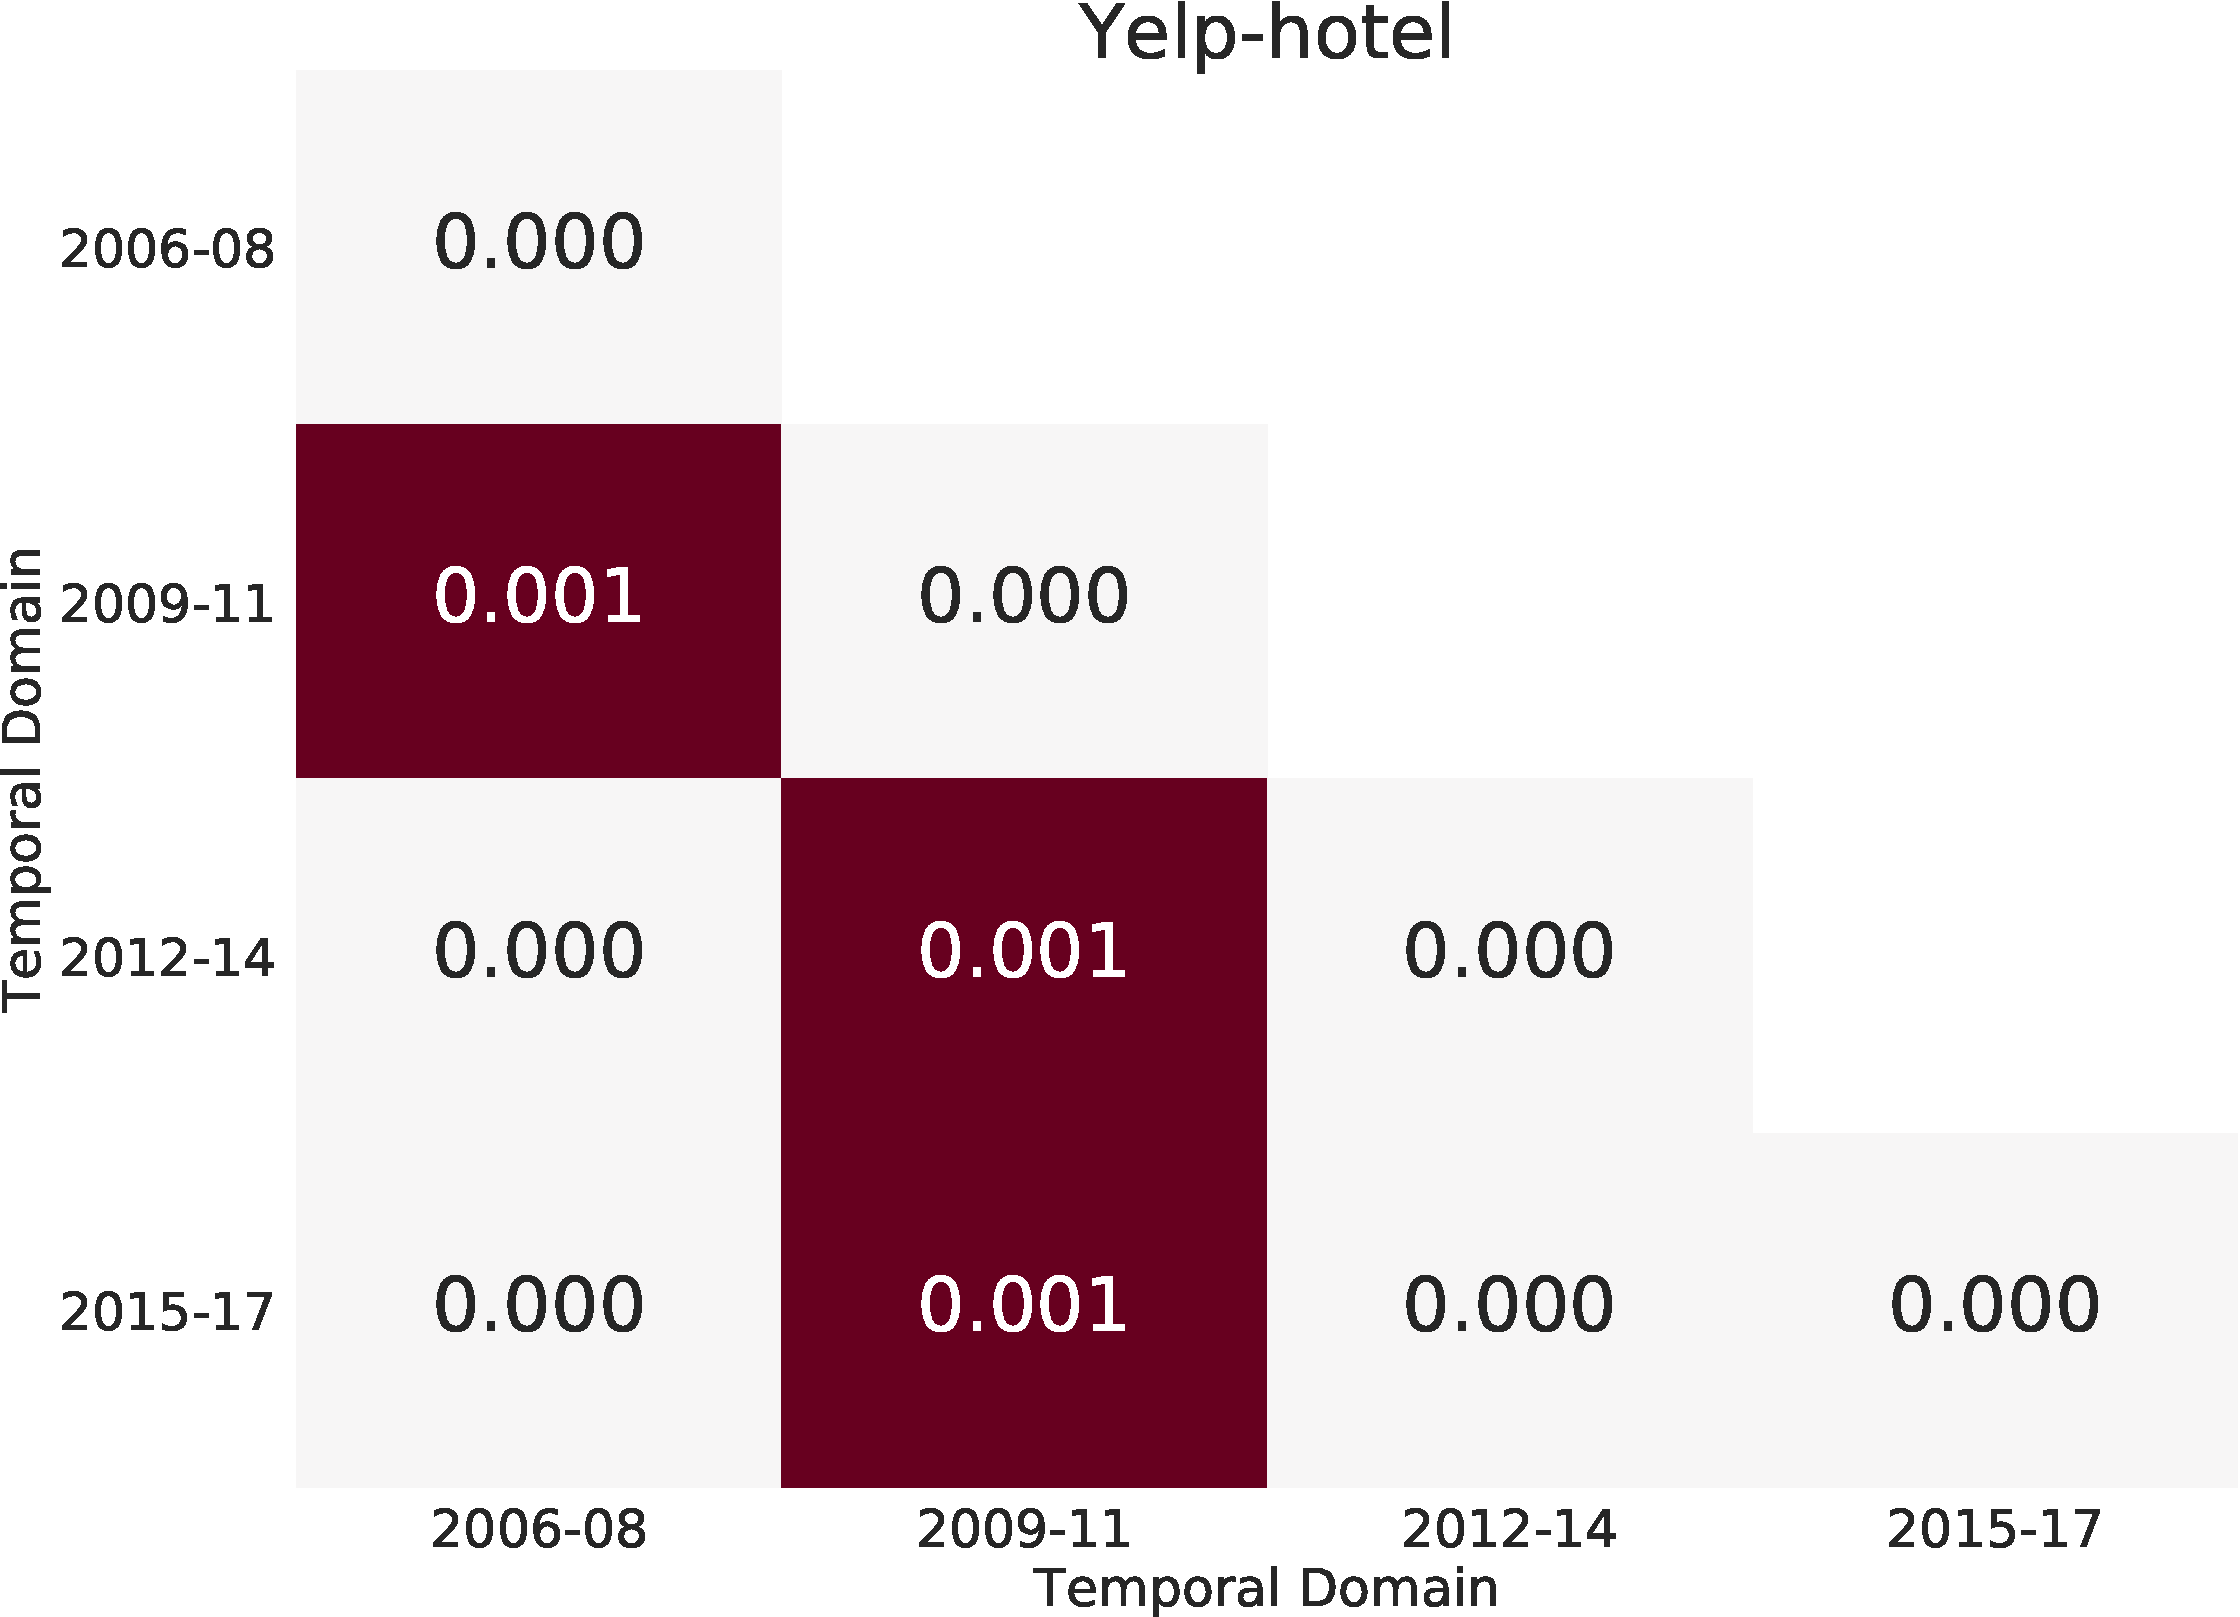
\includegraphics[width=0.43\textwidth]{images/chapter3/sm_shift/yelp_hotel_year_freq.pdf}
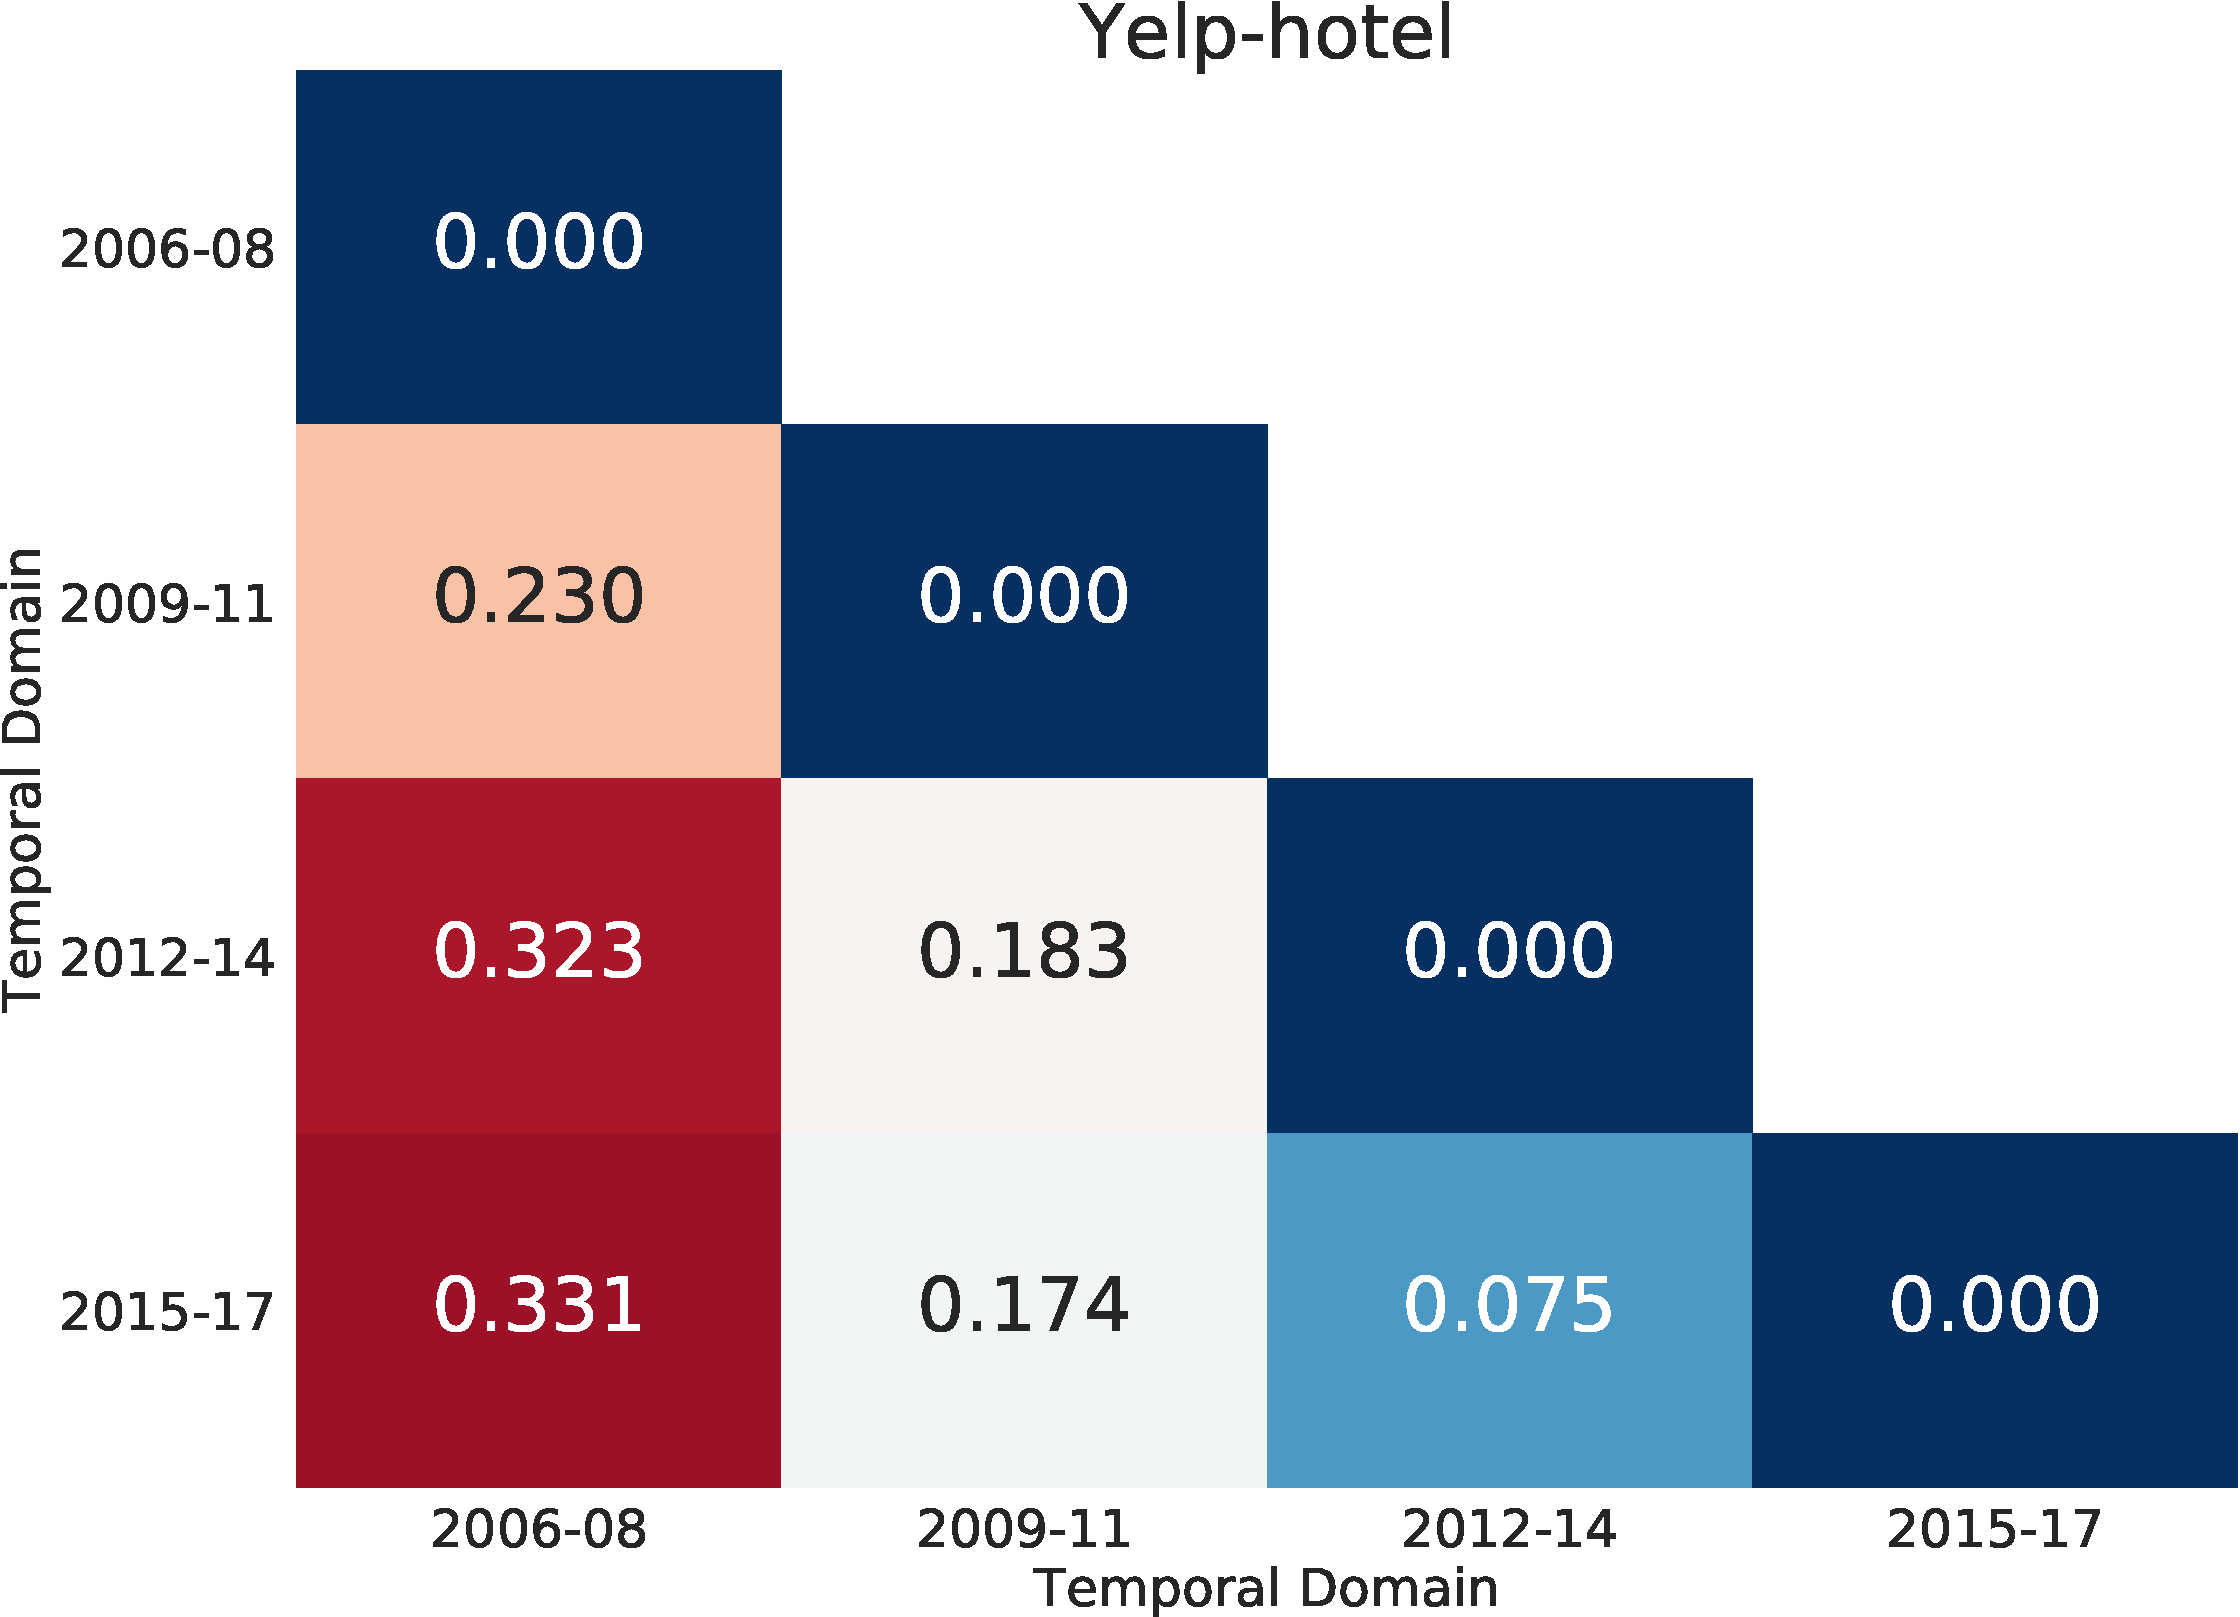
\includegraphics[width=0.43\textwidth]{images/chapter3/sm_shift/yelp_hotel_year_mi.pdf}
\caption{Semantic distribution shifts comparison between the top and most frequent words via Wasserstein distance. We present Yelp-hotel data for the illustration purposes and omit the other data due to space limits. The left is the semantic distribution shift for frequent words, the right is for top words ranked by mutual information. The higher score indicates higher shift.}
\label{chap3:fig:sm_shift}
\end{figure}

Using our proposed approach to constructing diachronic word embeddings,
we now consider how these embeddings can be used to further analyze language shift.

The Law of Conformity states a negative correlation between word frequency and meaning change~\cite{hamilton2016diachronic}; however, \cite{dubossarsky2017outta} show that the word frequency does play an important role in the semantic change, even though a small one. 
Diachronic embeddings have been used to measure the semantic shift using linear interpolation (regression)~\cite{hamilton2016diachronic}. 
Here, we re-examine this issue from another view, the distance of semantic distributions, which views the word embeddings as semantic distributions and measures how the word embeddings vary across time.

As in Section~\ref{chap3:subsec:ctt_shift},
we choose the top 1,000 important words ranked by mutual information, as well as a control group of the 1,000 most frequent words in each corpus.  We find that overlap between the 1,000 most important and most frequent words are 0\% across every dataset. This suggests that the most frequent words are not predictive for classification. 
We use our proposed method to train 200-dimensional diachronic word embeddings and extract diachronic word representations for both important and most frequent words, and leave 0s to the words that do not appear within a temporal interval. 
Finally, we use the Wasserstein distance~\cite{shen2018wasserstein} to measure the differences across temporal domains.
Wasserstein distance or Earth Mover's distance~\cite{vallender1974calculation} measures the distribution differences between source and target domains~\cite{shen2018wasserstein},
and thus here it measures semantic distribution shifts across time. 

We show temporal distribution shifts in Figure~\ref{chap3:fig:sm_shift}, 
and we observe two interesting findings. 
First, closer time intervals show less semantic distribution shift, which aligns with our analysis in Sections~\ref{chap3:subsec:wusage} and~\ref{chap3:subsec:ctt_shift}. Second, we observe that the frequent words have much smaller semantic distribution shifts than the top features selected by mutual information. 

To verify this second observation statistically, we conduct two-tailed t-test on the Yelp-hotel case to test our null hypothesis that the semantic distribution change is not significant. We separately compare the distribution distances of both frequent and top feature words with 0, which indicates no shift. Finally, the test results show p-value=0.076 for the frequent words and p-value=0.0038 for top feature words. Therefore, we reject the null hypothesis of top feature words at 95\% confidence level while we cannot reject the null hypothesis of frequent words.


\subsubsection{Comparing Different Ways to Measure Temporal Shifts}

\begin{table*}[ht]
\centering
\begin{tabular}{c||cccccc}
Correlation & Amazon  & Dianping & Economy & Twitter & Yelp-hotel & Yelp-rest \\\hline\hline
Usage-DD    & -.901* & .160    & -.106  & .028   & -.943*    & -.923*   \\
Context-DD  & -.989* & -.987*   & -.108  & .023   & -.949*    & -.960*  \\
Usage-Context  & .926* & -.009   & .600*  & .979*   & .950*    & .955*  
\end{tabular}
\caption{The correlations between word usages overlaps (Usage) and distribution distance (DD) as well as context overlaps (Context) and distribution distance (DD). The star sign (*) indicates p-value is less than .05.}
\label{chap3:tab:corr}
\end{table*}

We have presented language shifts across time domains based on word usage overlap (Section~\ref{chap3:subsec:wusage}), context overlap (Section~\ref{chap3:subsec:ctt_shift}), topic change (Section~\ref{chap3:subsec:topic}) and distribution distance (this section). However, it is not clear if these different metrics are measuring the same information. To understand this further, we calculate the Pearson correlation coefficient to measure the relationships between each pair of metrics. 
We show the correlations in Table~\ref{chap3:tab:corr}. We observe negative correlations between the two overlap measures (higher means more less shift) and distribution distance (lower means less shift),
and a positive correlation between word usage and context overlaps.
These results show that the three metrics are related, though there are some datasets where the correlations are low.


\subsection{Model for Temporality Adaptation}
\label{chap3:sec:model}

\begin{figure*}[tb!]
\centering
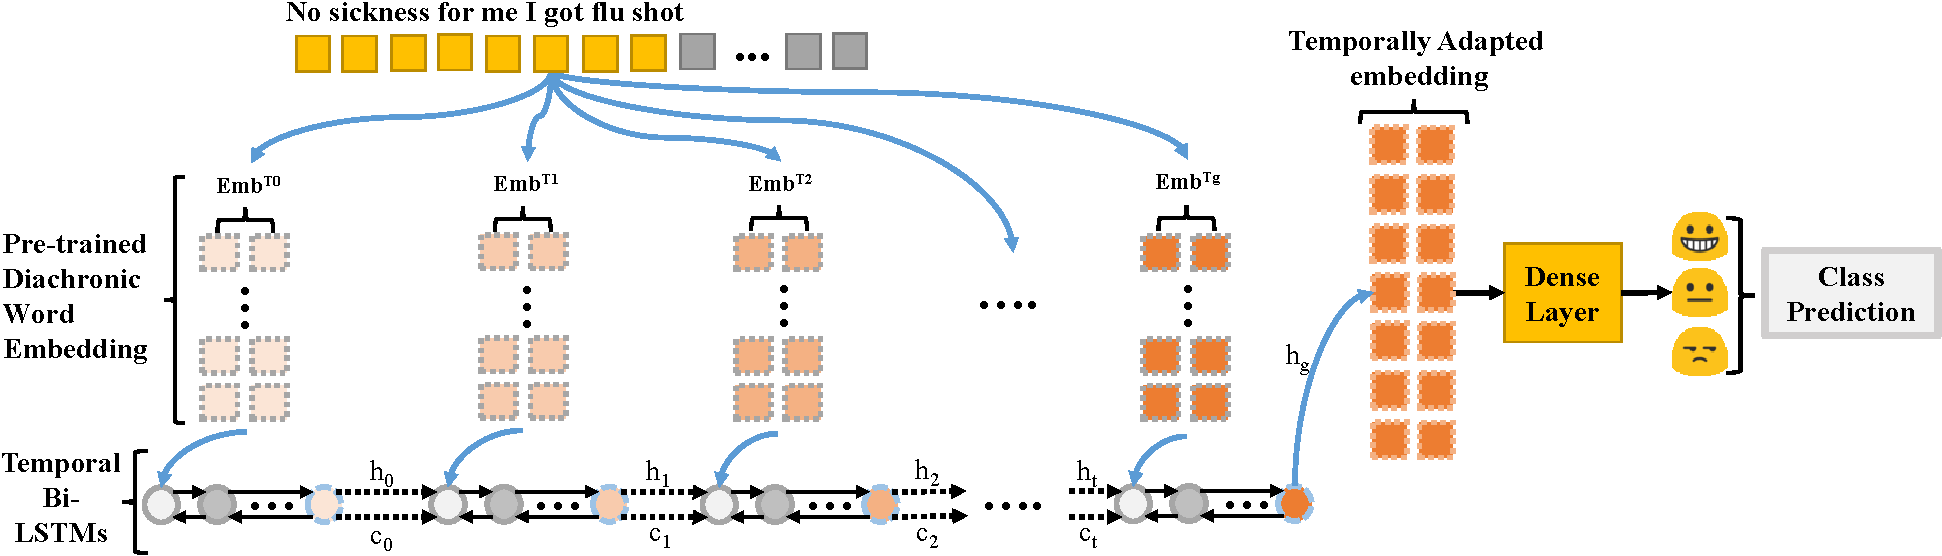
\includegraphics[scale=0.47]{./images/chapter3/model.pdf}
\caption{Architecture of the Neural Temporality Adaptation Model (NTAM). 
NTAM is initialized with $T$ diachronic word embeddings ($Emb^{Tt}, t\in T$) plus one general word embedding ($Emb^{Tg}$). The hidden state ($h_t, t\in T$) and memory cell ($c_t$) will excite and initialize the following Bi-LSTM. We feed the final hidden state ($h_g$, $g$ refers to general domain) to the following learning phase.}
\label{chap3:fig:model}
\end{figure*}

We construct a document classification model that assumes
the language used to describe document categories will evolve over time;
for example
newer documents may use emoji to express opinions,
while older documents would not contain these features.
%For example, people may switch from formal languages to emoji or other colloquial words or the ways to express opinions for a same document category would vary across time.
Our goal is to build document classifiers with time-invariant features and are thus robust to language shift. 

 %For the document classification task, the features used in training classifiers also change overtime such as word usage, contexts and distributional word representations.  Existing research shows that language shift impact on performances of document classifiers trained on the datasets cross multiple time intervals~\cite{huang2018examining}.

Our previous work~\cite{huang2018examining} on temporality adaptation for $n$-gram classifiers used a domain adaptation approach~\cite{daume2007frustratingly} where 
each time interval is treated as a domain.
This approach created $T$$+1$ versions of the feature set, one for each of the $T$ time domains, and one domain-independent feature set.
This allows the model to learn which features are associated with specific domains, while the domain-independent parameters can be used for future data.
We analogously apply this idea to the neural setting, where we construct $T$$+1$ different representations, at both the word level (using diachronic word embeddings) and the document level.
Moreover, we use a time-driven learning process that models
the shift of word representations as a gradual process of adapting representations to new data while starting with old information.

We thus present the {\bf Neural Temporality Adaptation Model (NTAM)} (Figure~\ref{chap3:fig:model}) based on three strategies: diachronic word embeddings (Section~\ref{chap3:sec:dwe}), $T+1$ views of inputs, and a time-driven learning process.
This model can learn language shifts and time invariant representations of documents for classification.

\paragraph{T+1 views of inputs.}
Analogous to the approach of \cite{daume2007frustratingly} for non-neural classifiers, 
we create $T+1$ word representations, where $T$ refers to the number of diachronic domain embeddings and 1 refers to a general embedding, which trains word embeddings on the whole corpus without time labels. Our intuition is to use time-specific embeddings to provide documents from different time intervals with different views of semantic meaning. 
We train diachronic word embeddings using our proposed method via fastText, though we also experiment with other approaches. 
We initialize the model with the domain-specific embeddings and the general word embedding. The model will encode input documents into $T+1$ views of word representations. 
The $T+1$ embeddings provide diverse views of input words, which are fed to the rest of the neural architecture, leaving the model to optimize representations automatically.

\paragraph{Time-driven learning process.}
To learn temporal variations for document representations, we propose a series of $T+1$ continuously temporal Bidirectional Long Short Term Memory (Bi-LSTM) models~\cite{hochreiter1997long}. The first $T$ Bi-LSTMs correspond to the $T$ time domains and the last Bi-LSTM corresponds to the general view of input documents and outputs the final document representation. Similar to how the diachronic word embeddings encode input words into multiple views of time domains, we use $T+1$ Bi-LSTMs to learn diachronic views of document representations. 
%Thus, each layer could learn a different view of document representation. 

To capture the semantic shifts across time domains, our intuition is to model the dynamic process. The memory mechanism of LSTM fits our need, which optimizes the balance across different time patterns via non-linear computations. While each Bi-LSTM reads through tokens in its own input document, we feed the previous Bi-LSTM's hidden state and memory cell to excite the learning process of the subsequent Bi-LSTM. The final Bi-LSTM learns jointly the previous shift patterns of document representations with the general embedding view of documents and outputs its final document representation $h_g$. 

The final document representation is fed into a dense layer with a non-linear activation function. We use outputs of the dense layer for document class prediction,
where we use one-hot encoding to represent document labels and use the softmax function for class predictions. Finally, we use categorical cross-entropy as the loss function.



\subsection{Experiments}
\label{chap3:sec:dweExp}

We conduct experiments on the task of document classification.
We split the data chronologically to simulate the realistic scenario where a classifier is trained on older data and tested on newer data. 
Thus, the first $T-1$ time domains are used for training;
the last time domain is split into two equal-sized sets for development and testing.
The final data details are described in Table~\ref{chap3:table:statics}.

\begin{table}[ht]
 \centering
 %\resizebox{\columnwidth}{!}{
    \begin{tabular}{c|ccc}
    \hline\hline
    Datasets & Train & Dev. & Test\\
    \hline
    Amazon & 59,399 & 11,880 & 11,880 \\
    Dianping & 503,330 & 83,889 & 83,889 \\
    Economy & 4,774 & 596 & 596\\
    Twitter & 1,632 & 272 & 272\\
    Yelp-hotel & 20,975 & 6,993 & 6,993 \\
    Yelp-rest & 106,943 & 35,648 & 35,648 \\
    \hline
    \end{tabular}
    %}
    \caption{Data statistics of the six corpora. We show the number of documents in each split.}
    \label{chap3:table:statics}
\end{table}


\subsubsection{Implementation and Training}
We implement classification models using Keras~\cite{chollet2015keras} and scikit-learn~\cite{pedregosa2011scikit}. We select the top 15K words by frequency and set the other words as ``unk''. The models are trained for 15 epochs with the batch size of 64. Each document is padded to 60 tokens. We set the Bi-LSTM output to 200 dimensions. We choose ReLU~\cite{hahnloser2000digital} as the activation function of the dense layer and 0.2 as our default dropout rate~\cite{srivastava2014dropout}. The dense layer outputs 200 dimensions for final document class prediction. We select cross-entropy as our default loss function, and we optimize model parameters via RMSprop~\cite{tieleman2012lecture} with the learning rate as 0.0001. Unless otherwise stated, we leave the other parameters as defaults.

\subsubsection{No Adaptation Baselines}
To ensure fair comparisons, we use the same settings across all models. We compare our proposed model to seven baselines, where three standard classifiers do not perform temporality adaptation.

\paragraph{LR.} 
We extract 1- and 2-gram features on the corpora with the most frequent 15K features. We then build a logistic regression classifier using \texttt{LogisticRegression} from scikit-learn~\cite{pedregosa2011scikit} with default parameters.

\paragraph{CNN.} 
We implement the Convolutional Neural Network (CNN) classifier described in~\cite{kim2014convolutional}. To keep consistent, we initialize the model with pre-trained word embeddings~\cite{bojanowski2017enriching} that were trained on the same datasets as the diachronic embeddings. We only keep the 15K most frequent words and replace the rest with an ``unk'' token. We set model optimizer as Adam~\cite{kingma2014adam}. 

\paragraph{Bi-LSTM.} 
We build a bi-directional Long Short Term Memory (bi-LSTM)~\cite{hochreiter1997long} classifier to examine the effectiveness of temporal learning process in our proposed model. The classifier is initialized with the pre-trained word embeddings.

\subsubsection{Domain Adaptation Baselines}

\paragraph{FEDA.} 
Following \cite{huang2018examining} we adapt for time domains using the ``frustratingly easy'' domain adaptation (FEDA) method~\cite{daume2007frustratingly}. 
The feature set is augmented such that each feature has a domain-specific version of the feature for each time domain, as well as a general domain-independent version of the feature.
The values of features are set to the original feature value for the domain-independent feature and the domain-specific features that apply to the document, while domain-specific features for documents that do not belong to that domain are set to $0$.
At test time, we only use the general, domain-independent features. 
We use the same feature extraction procedures and the same logistic regression classifier as the \textit{LR} baseline.

\paragraph{DANN.} 
We consider the domain adversarial training network~\cite{ganin2016domain} (DANN) on the time adaptation task. We re-implement the same network and set domain prediction as predicting the time domain label while keeping the document label prediction as the default. We use the model from the epoch when the model achieves the best result on the development set for the final model.

\paragraph{RCNN \& HAN.} 
He et al.~\cite{he2018time} propose an evolving framework to train document classifiers. We re-implement two classifiers, RCNN and HAN with diachronic propagation learning strategy, which achieved the best performances in their paper. The RCNN~\cite{lai2015recurrent} classifier integrates both LSTM and CNN, and the HAN~\cite{yang2016hierarchical} classifiers uses hierarchical attention neural architectures. We keep the two models with the same parameters as their open sourced code and initialize the two models with pre-trained 200 dimensional word embeddings~\cite{bojanowski2017enriching}. We apply Adam and RMsprop for RCNN and HAN respectively, because the two optimizers perform much better on validation sets than the stochastic gradient descent optimizer used in the original paper. The work is close to our work but there are three major differences:
\begin{itemize}
    \item Time invariance. We train one unified model with diachronic adaptation by using a time-independent representation (the 1 of the $T+1$ representations) to learn a time-invariant classifier that can be used for future data. In contrast, these baselines learn $T-1$ models, where they train one model for each time domain.
    \item Diachronic word embeddings. Our method uses diachronic word embeddings to encode inputs in $T+1$ different views. The baseline encoding is based on only the current embedding space and therefore might not capture embedding shifts over time.
    \item Learning process. The baseline learns a weighted sum between the intermediate layer's outputs between the previous model and the current model. In contrast, we deploy the $T+1$ Bi-LSTMs to jointly learn time dependencies across all time intervals. %We approach the time problem by using previous diachronic view to excite the next learning phase.
\end{itemize} 

% \begin{table*}[ht]
% \centering
% \resizebox{\textwidth}{!}{
% \begin{tabular}{c||ccc||ccccc||cc}
%  & \multicolumn{3}{c||}{No-Adaptation baselines} & \multicolumn{5}{c||}{Adaptation baselines} & \multicolumn{2}{c}{Our Model} \\
% Data & LR & CNN & Bi-LSTM & FEDA & DANN & HAN & RCNN & RCNN+d & NTAM & NTAM+d\\\hline\hline
% Twitter & .874 & .873 & .879 & .890 & .851 & .847 & .869 & .861 & .863 & \textbf{.898} \\
% Economy & .699 & .707 & .692 & .686 & .687 & .690 & .697 & .701 & .708 & \textbf{.711} \\
% Yelp-rest & .818 & .756 & .787 & \textbf{.831} & .736 & .794 & .782 & .805 & .785 & .828 \\
% Yelp-hotel & .773 & .753 & .758 & \textbf{.811} & .733 & .740 & .762 & .760 & .784 & .790 \\
% Amazon & .778 & .762 & .771 & .782 & .686 & .748 & .782 & .787 & .787 & \textbf{.808} \\
% Dianping & .710 & .715 & .706 & .687 & .686 & .699 & .692 & .702 & .696 & \textbf{.738}
% \end{tabular}
% }
% \caption{Performances table of baselines and our proposed model. We evaluate the methods via F1-weighted score. For each dataset, the best score is bolded. ``+d'' refers to initialize our proposed model by our diachronic embeddings\textcolor{red}{, while the NTAM only initializes with normal word embeddings}.}
% \label{chap3:tab:results}
% \end{table*}

\begin{table*}[t]
\centering
\begin{tabular}{c||ccc||cccc||c}
 & \multicolumn{3}{c||}{Baselines (No adaptation)} & \multicolumn{4}{c||}{Baselines (Adaptation)} & Our Model \\
Data & LR & CNN & Bi-LSTM & FEDA & DANN & HAN & RCNN & NTAM\\\hline\hline
Twitter & .874 & .873 & .879 & .890 & .851 & .847 & .869 & \textbf{.898} \\
Economy & .699 & .707 & .692 & .686 & .687 & .690 & .697 &  \textbf{.711} \\
Yelp-rest & .818 & .756 & .787 & \textbf{.831} & .736 & .794 & .782 & .828 \\
Yelp-hotel & .773 & .753 & .758 & \textbf{.811} & .733 & .740 & .762 & .790 \\
Amazon & .778 & .762 & .771 & .782 & .686 & .748 & .782 & \textbf{.808} \\
Dianping & .710 & .715 & .706 & .687 & .686 & .699 & .692 & \textbf{.738}
\end{tabular}
\caption{Performance of different models evaluated with weighted F1 scores. For each dataset, the best score is bolded. 
LR and FEDA are non-neural $n$-gram models, while the others are neural models.
%``+d'' refers to initialize our proposed model by our diachronic embeddings, while the NTAM only initializes with normal word embeddings}.
}
\label{chap3:tab:results}
\end{table*}


\begin{table*}[t]
\centering
\begin{tabular}{c||cccc||cccc}
 & \multicolumn{4}{c||}{RCNN} & \multicolumn{4}{c}{NTAM} \\
Data & Incre & Linear & Procrustes & Subword & Incre & Linear & Procrustes & Subword\\\hline\hline
Twitter & -0.7 & +1.4 & -0.2 & -0.8 & +1.4 & -0.3 & +1.7 & +3.5\\
Economy & +0.5 & 0.0 & -0.7 & +0.4 & -0.3 & -1.0 & -0.5 & +0.3\\
Yelp-rest & +1.4 & +0.1 & -1.9 & +2.3 & +1.9 & +1.6 & +1.4 & +4.3\\
Yelp-hotel & -1.5 & -1.2 & -0.5 & -0.2 & -0.7 & -2.0 & -1.8 & +0.8\\
Amazon & +0.2 & +0.2 & -2.0 & +0.5 & -0.8 & -0.7 & -0.8 & +2.1\\
Dianping & +0.4 & +1.6 & +0.7 & +1.0 & +0.8 & +1.8 & +3.4 & +4.2\\\hline\hline
Average & 0.05 & 0.35 & -0.47 & 0.53 & 0.38 & -0.10 & 0.57 & 2.53\\
Median & 0.30 & 0.15 & -0.60 & 0.45 & 0.25 & -0.50 & 0.45 & 2.80\\
\end{tabular}
\caption{Performance gains of two neural temporality adaptation models when they are initialized by diachronic word embeddings as compared to initialization with standard non-diachronic word embeddings. \textit{Subword} refers to our proposed diachronic word embedding in this chapter (Section~\ref{chap3:sec:dwe}). We report absolute percentage increases in weighted F1 score after applying diachronic word embeddings.}
\label{chap3:tab:dia}
\end{table*}


\subsubsection{Results}
\label{chap3:sec:results}


The results of our experiments are show in Table~\ref{chap3:tab:results}. 
Our proposed approach leads to performance improvements over the comparable baselines on most datasets.
NTAM has the highest performance on 4 out of 6 datasets, while FEDA has the highest performance on the other 2 (while NTAM is the next best for those 2).


The baselines with domain adaptation generally obtain a small performance boost over the baselines without adaptation on temporality. 
Among the non-neural models, the adaptation baseline FEDA outperforms the non-adaptation baseline LR on 4 out of 6 datasets. 
Among the neural models, the best adaptation baseline outperforms the best non-adaptation baseline on 3 out of 6 datasets,
with the RCNN generally outperforming the other baselines.
%The RCNN generally shows improvements over the other neural non-adaptation models on the Yelp and Amazon datasets. 
This indicates that the temporal factor can potentially improve the performance of document classification, and that domain adaptation is a possible approach to temporality adaptation. 

\paragraph{Significance analysis.} 
To verify the improvements of our proposed method NTAM compared to baselines, we conduct a significance analysis to compare our proposed model with the RCNN, which is the closest model to ours. We follow \cite{berg2012empirical} and bootstrap sample 50 pairs of test datasets with replacement. We keep the same data size as the previous experiments in the Table~\ref{chap3:tab:results}. We then use the same previous parameters and re-conduct the classification experiments. We format the experimental results as two lists of scores. We conduct a paired t-test to test the null hypothesis that our proposed model does not differ significantly from the RCNN. The test presents a significant result with t(95) = 3.258 and p = 0.00119. The result suggests rejecting the null hypothesis at a 95\% confidence level.

%\paragraph{Diachronic vs. general word embedding.} To explore the effectiveness of the diachronic word embedding, we compare the performance between diachronic and general word embeddings. We apply both types of word embeddings on the two temporality adaptation models, RCNN and NTAM. The NTAM initialized by diachronic word embedding obtains a small performance boost than the one initialized with general word embedding in main datasets. And the diachronic word embeddings also improve the RCNN in 4 out of 6 datasets. This indicates that diachronic word embedding plays an effective role in improving performances of the document classifier.


\subsection{Effectiveness of Diachronic Embeddings}

Lastly we investigate how diachronic word embeddings affect classifiers.
While NTAM used diachronic word embeddings and other baselines did not,
we also compare to a version of NTAM initialized with regular word embeddings (to understand whether diachronic embeddings are important to the model's performance),
and we also experiment with combining diachronic embeddings with a baseline model (to understand if diachronic embeddings can be used in other classifiers).


We also compare different methods of constructing diachronic word embeddings. In addition to our proposed method in Section~\ref{chap3:sec:dwe}, which uses subword embeddings via fastText,
we consider three other approaches (Section~\ref{chap3:subsec:dweBaselines}).
We use incremental training~\cite{kim2014temporal} (abbreviated \textit{Incre}, using fastText),
linear regression~\cite{kulkarni2015statistically}, implemented in scikit-learn,
and Procrustes~\cite{hamilton2016diachronic}, implemented in SciPy.
We keep the same fastText parameters as in previous experiments and train a word embedding model separately for each time domain, then align the pre-trained embeddings to get final diachronic word embeddings. We then re-run the classification task with the new diachronic word embeddings. 

Table~\ref{chap3:tab:dia} shows the absolute percentage improvement in classification performance when using each diachronic embedding compared to a classifier without diachronic embeddings.
Overall, diachronic embeddings improve classification models.
The diachronic embedding appears to be particularly important for NTAM, improving performance on all 6 datasets with an average increase in performance up to 2.53 points.
The RCNN also benefits from diachronic embeddings, but to a lesser extent, with an improvement on 4 of the 6 datasets.
Comparing the different methods for constructing diachronic embeddings,
we find that our proposed subword method works the best on average for both classifiers. The incremental training method also provides improved performance for both classifiers, while the linear regression and Procrustes approaches have mixed results.

% % \paragraph{Temporality adaptation} is to integrate temporal factor into classification models. Particularly, in this work, we focus on the task of document classification. \newcite{huang2018examining} use feature augmentation methods~\cite{daume2007frustratingly} to train time-invariant logistic regression classifiers. \newcite{he2018time} propose a time-evolving training framework that continuously trains T number of models across T time intervals.

% \textcolor{red}{\textbf{Domain adaptation} aligns source with related target distributions to obtain more generalized feature representations and classifiers~\cite{daume2007frustratingly, ganin2016domain}. Methods of domain adaptation exist to adjust domain variations~\cite{shen2018wasserstein}. However, time is not explicitly considered into the adaptation process. \newcite{huang2018examining} explore \textit{temporality adaption} via feature augmentation~\cite{daume2007frustratingly}. In this study, we propose a simple training method of diachronic word embeddings and extend their work from traditional classifiers to neural models.}

\section{Conclusion}
\label{chap3:sec:conclusion}

In this chapter, we proposed two temporality adaptation methods to improve the temporal robustness of document classifiers via the feature augmentation and diachronic word embedding.
We explore and examine language temporal shifts on seven bilingual corpora from social media to news articles in Section~\ref{chap3:sec:data}. 
As described in Section~\ref{chap3:sec:fa}, We have shown both qualitatively and quantitatively that our proposed FEDA and diachronic word embedding are capable of discovering language shift patterns and improve model productiveness across both seasonal and non-seasonal time periods.
We proposed a new framework to train diachronic word embedding and evaluated the embedding model with existing methods.
The Section~\ref{chap3:sec:model} presented a new time-driven classification model that encodes documents through the diachronic word embedding. 


\chapter{User Factor Adaptation}
\label{chp:user}

The previous Chapter~\ref{chp:temporality} has examined language shifts and presented two temporality adaptation approaches for the document classification task. 
It has shown the effectiveness of domain adaptation with the document metadata, time.

In this chapter, we 

\section{Introduction}
% demographic factors exist in text documents
Different demographic groups can show substantial linguistic variations, especially in online data~\cite{goel2016social,johannsen2015cross}. 
%Such demographic factors have significant impacts on language use in people's word expression~\cite{goel2016social}, syntax~\cite{johannsen2015cross}, etc. 
These variations can affect natural language processing models such as sentiment classifiers.
For example, researchers found that women were more likely to use the word \textit{weakness} in a positive way, while men were more likely to use the word in a negative expression~\cite{volkova2013exploring}.

Models for text classification,
the automatic categorization of documents into categories, 
typically ignore attributes about the authors of the text.
With the growing amount of text generated by users online, whose personal characteristics are highly variable,
there has been increased attention to how user demographics are associated with the text they write.
Promising recent studies have shown that incorporating demographic factors can improve text classification~\cite{volkova2013exploring,hovy2015demographic,yang2017overcoming, li2018towards}. 
\cite{lynn2017human} refer to this idea as {\em user factor adaptation}
and proposed to treat this as a domain adaptation problem in which demographic attributes constitute different domains.
We extend this line of work in a number of ways:

\begin{itemize}
\item We assemble and publish new datasets containing four demographic factors: gender, age, country, and US region. The demographic attributes are carefully inferred from profile information that is separate from the text data.
%Our data could be used for tasks beyond this work, such as the study of algorithmic bias.
\item We experiment with neural domain adaptation models~\cite{ganin2016domain}, which may provide better performance than the simpler models used in prior work on user factor adaptation.
We also propose a new model using a multitask framework with adversarial training.
\item Our approach requires demographic attributes at training time but not at test time: we learn a single representation to be invariant to demographic changes.
This approach thus requires fewer resources than prior work.
%which is important since demographic attributes are often unavailable.
\end{itemize}

In this study, we treat adapting across the demographic factors as a domain work problem, in which we consider each demographic factor as a domain. We focus on four different demographic factors (gender, age, country, region) in four English-language social media datasets (Twitter, Amazon reviews, Yelp hotel reviews, and Yelp restaurant reviews), which contain text authored by a diversity of demographic groups.

%In this study, we treat modeling the demographic factors as a domain adaptation question, which we consider each demographic factor as a domain. We focus on four different demographic factors, gender, age, country, region, on four English-language social media datasets, Twitter, Amazon, Yelp hotel and restaurant reviews, which usually own diverse demographic communities. Particularly, we examine and investigate the following two questions:
%
%\begin{itemize}
%    \item Does language show demographic variations in social media data?
%    \item How to model demographic variations in the process of text classification?
%\end{itemize}
%

We first conduct an exploratory analysis of how different demographic variables are associated with documents and document labels (Section~\ref{sec:exploratory}).
%To address the questions, we first qualitatively explore and compare linguistic patterns on topic distributions across four different demographic factors, gender, age, country, region. We build machine learning classifiers on the domain attributes and evaluate how predictable of language could help categorize the demographic identities. 
We then describe a neural model for the task of document classification that adapts to demographic factors using a multitask learning framework (Section~\ref{sec:model}). Specifically, the model is trained to predict the values of the demographic attributes from the text in addition to predicting the document label. 
%we treat the training process as  \textit{K + 1} prediction tasks, which refers to the label prediction as well as the K demographic domain tasks. For example, the gender domain task predicts if a female or male user generates the text. 
Experiments on four social media datasets show that user factor adaptation is important for document classification, and that the proposed model works well compared to alternative domain adaptation approaches (Section~\ref{sec:experiments}).




\section{Related Work}

\paragraph{Domain adaptation} tries aligning source with related target distributions to obtain more generalized feature representations and classifiers. For the text classification task, there are two conventional methods, feature augmentations~\cite{daume2007frustratingly, blitzer2006domain, huang2018examining} and domain adversarial training~\cite{ganin2016domain, chen2016adversarial, liu2017adversarial}. However, one issue with the proposed methods is they did not consider the user demographic factors, which show strong variations among social media documents. Additionally, most of the adaptation only work on two different domains, but the demographic factors have more complex domains and divergent differences between domains.

\paragraph{User factor adaptation} integrates demographic factors into the machine learning classifiers. The demographic factors usually refer to the attributes of users, such as gender, age, geographic location, etc. Online generated user texts show demographic variations in the linguistic styles, and the linguistic style differences could be used for the use factor prediction~\cite{rosenthal2011age, zhang2016predicting, hovy2018improving}. The user factors impact on how online users express their opinions and show promising improvements in the text classification task~\cite{volkova2013exploring, hovy2015demographic, lynn2017human, yang2017overcoming}. The closest work to our study~\cite{lynn2017human} created general and domain-specific features to train a more generalized classification model. However, such a method heavily suffers extremely high feature dimensions and handcraft features. 



\section{User Factor Adaptation via Multitask Learning}
\label{sec:exploratory}

We begin with an empirical analysis of how text is related to various demographic attributes of its authors. We first present a description of the demographic attributes. We then conduct qualitative analyses of demographic variations within the collected data on three cascading levels: document, topic and word.
The goal is to get a sense of the extent to which language data varies across different user factors and how these factors might interact with document classification. 
This will motivate our adaptation methods later
and provide concrete examples of the user factors that we have in mind.


\subsection{Data}
We experiment with four corpora from three social media sources:
\begin{itemize}
\setlength\itemsep{0ex}
    \item {\bf Twitter:} Tweets were labeled with whether they indicate that the user received an influenza vaccination (i.e., a flu shot)~\cite{huang2017examining},
    used in a recent NLP shared task~\cite{W18-5904}.
    \item {\bf Amazon:} Music reviews from Amazon labeled with sentiment.
    \item {\bf Hotel:} Hotel reviews from Yelp labeled with sentiment.
    \item {\bf Restaurant:} Restaurant reviews from Yelp labeled with sentiment.
\end{itemize}
The latter three datasets were collected for this study.
All documents are given binary labels.
For the Amazon and Yelp data, we encode reviews with a score $>$$3$ (out of 5) as positive and $\leq$$3$ as negative.
For the Yelp data, we removed reviews that had fewer than ten tokens or a helpfulness/usefulness score of zero. 


\subsubsection{User Attribute Inference}

Previous work on user factor adaptation considered the factors of gender, age, and personality~\cite{lynn2017human}.
We similarly consider gender and age, and instead of personality, we consider a new factor of geographic location.
For location, we consider two granularities as different factors, country and region.

These factors must be extracted from the data.
One of our goals is to infer these factors
in a way that is completely independent of the text used for classification.
This is in contrast with the approach used in~\cite{lynn2017human},
who inferred the attributes from the text of the users,
which could arguably confound the interpretation of the results,
as domains are defined using the same information available to the classifier.
Thus, we used only information from user profiles to obtain their demographic attributes.


%\vspace{-.5ex}
\paragraph{Gender and Age.} We inferred user gender and age through the user's profile image using the Microsoft Facial Recognition API.\footnote{\url{https://azure.microsoft.com/en-us/services/cognitive-services/face/}}
Recent comparisons of different commercial face APIs have found the Microsoft API to be the most accurate~\cite{jung2018assessing} and least biased~\cite{buolamwini2018gender}.
We filtered out users that are inferred to be younger than 12 years old. If multiple faces are in an image, we used the first result from the API. 
Gender is encoded with two values, male and female. 
For simplicity, we also binarized the age values ($\leq$$30$ and $>$$30$).

%\vspace{-.5ex}
\paragraph{Country and Region.} 
We define two factors based on the location of the user.
For the Twitter data, we inferred the location of each user with the Carmen geolocation system~\cite{dredze2013carmen},
which resolves the user's location string in their profile to a structured location. Because this comes from the user profile, it is generally taken to be the ``home'' location of the user.
For Amazon and Yelp, we collected user locations listed in their profiles,
then used pattern matching and manual whitelisting to resolve the strings to specific locations (city, state, country). 
To construct user factors from location data,
we first created a binary country variable
to indicate if the user's country is the United States (US, the most common country in the data) or not. 
Among US users, we resolved the location to a region.
We follow the US Census Bureau's regional divisions~\cite{branch_2012} to categorize the users into four regional categories: Northeast (NE), Midwest (MW), South (S) and West (W). We labeled Washington D.C. as northeast in this study;
we excluded other territories of the US, such as Puerto Rico and U.S. Virgin Islands, since these locations do not contain much data and do not map well to the four regions.

%\vspace{-.5ex}
\paragraph{Accuracy of Inference}

Attributes inferred with these tools will not be perfectly accurate. 
Although such inaccuracies could lead to suboptimal training,
this does not affect our classifier evaluation,
since we do not use demographic labels at test time.
%Our goal is to see if including these attributes during training can lead to more robust classifiers.
Nonetheless, we provide a rough estimate of the accuracy of the attributes extracted from faces.
We randomly sampled 100 users across our datasets.
Two annotators reviewed each image and guessed the gender and age of the user (using our binary categories) based on the profile image.
A third annotator chose the final label when the first two disagreed (annotators disagreed on gender in 2\% of photos and age in 15\% of photos).
Our final annotations agreed with the Face API's gender estimates 88\% of the time across the four datasets (ranging from 84\% to 100\%),
and age estimates 68\% of the time across the four datasets (ranging from 56\% to 92\%).


%For location, Carmen is reported to be over 90\% accurate at the country level~\cite{dredze2013carmen}.
%It was only 65\% accurate at the state level, although this was evaluated across the entire world and may be more accurate within the US.

\begin{table*}[t]
\centering
\resizebox{\textwidth}{!}{
\begin{tabular}{c||c|c||cc|cc|cc|cccc}
\multirow{2}{*}{} & \multirow{2}{*}{\begin{tabular}[c]{@{}c@{}}\# Docs\\ \end{tabular}} & \multirow{2}{*}{\begin{tabular}[c]{@{}c@{}}\# Users \\ \end{tabular}} & \multicolumn{2}{c}{Gender} & \multicolumn{2}{|c}{Age} & \multicolumn{2}{|c}{Country} & \multicolumn{4}{|c}{Region} \\
 &  &  & F & M & $\leq$30 & \textgreater{}30 & US & $\lnot$US & NE & MW & S & W \\\hline
Twitter & 9.8K & 9.8K & .575 & .425 & .572 & .428 & .772 & .228 & .104 & .120 & .145 & .631 \\
Amazon & 40.4K & 34.3K & .333 & .667 & .245 & .755 & .900 & .100 & .097 & .096 & .132 & .675 \\
Hotel & 169K & 119K & .576 & .424 & .450 & .550 & .956 & .044 & .297 & .166 & .271 & .266 \\
Restaurant & 713K & 811K & .547 & .453 & .451 & .549 & .892 & .108 & .305 & .181 & .302 & .212
\end{tabular}
}
\caption{Dataset statistics including user demographic distributions for four user factors.}
\label{tab:demographic}
\end{table*}

\subsubsection{Data Summary}
We show the data statistics along with the full demographic distributions in the Table~\ref{tab:demographic}.
While our study does not require a representative sample from the data sources,
since our primary goal is to evaluate whether we can adapt models to different demographics,
we observe some notable differences between the demographics of our collection and the known demographics of the sources.
Namely, the percentage of female users is much higher in our data than among Twitter users~\cite{tien_2018} and Yelp users~\cite{yelp_2018} as estimated from surveys. 
This discrepancy could stem from our process of sampling only users who had profile images available for demographic inference,
since not all users provide profile photos,
and those who do may skew toward certain demographic groups~\cite{rose2012face}.
%MP: Cutting this explanation for space
%For example, research on ``impression management''~\cite{rose2012face} found that young people actively maintain their self-selected social media displays, especially young women, which may explain why more profile images were inferred to be female than male. 

%We could find that the higher percentage of females than males in the collected Twitter and Yelp data while the collected Amazon data shows male percentage is almost twice than the female. 

%MP: Amazon is harder to explain, so I'm going to leave this out
%According to the Amazon survey\footnote{\url{https://www.statista.com/statistics/747895/us-amazon-prime-membership-gender/}}, our collected data show significantly fewer females. 

%MP: I'm going to move this into the attribute section. We already had a citation for the performance of face APIs and I will move this citation to the same sentence.
%\subsection{Label Evaluation. }
%Comparing to Face++, IBM and Amazon, Microsoft Face API wins the best accuracy in gender and age classification tasks~\cite{jung2018assessing}. This suggests 


\subsubsection{Privacy Considerations}

While our data collection includes only public data, 
due to the potential sensitivity of user profile information,
we stored only data necessary for this study.
Therefore, we anonymized the personal information and deleted user images after retrieving the demographic attributes from the Microsoft API. We only include aggregated information in this paper and do not publish any private information associated with individuals including example reviews. 
The dataset that we share will include our model inferences but not the original image data; instead, the dataset will provide 
instructions on how the data was collected in enough detail that the approach can be replicated.


%\subsection{Are user demographic factors predictable by linguistic behaviors?}
\subsection{Are User Factors Encoded in Text?}
\label{subsec:analysis}

It is known that the user factors we consider are associated with variability in language, including in online content~\cite{hovy2015demographic}.
For example, age affects linguistic style~\cite{wagner2012age},
and language styles are highly associated with the gender of online users~\cite{hovy2018capturing}.
Dialectical differences also cause language variation by location;
for example, ``dese'' (these) is more common among social media users from the Southern US than other regions of the US~\cite{goel2016social}.

Our goal in this section is to test
whether these variations hold in our particular datasets,
how strong the effects are,
and which of our four factors are most associated with language.
We do this in two ways,
first by measuring predictability of factors from text,
and second by qualitatively examining topic differences across user groups.


\begin{table}[t]
\centering
\resizebox{.7\columnwidth}{!}{
\begin{tabular}{c|c|c|c|c}
 & Gender & Age & Country & Region \\\hline
Twitter & +9.6 & +15.3 & +9.0 & +3.3 \\
Amazon & +15.2 & +12.2 & +18.0 & +13.0 \\
Hotel & +17.2 & +10.9 & +25.4 & +11.6 \\
Restaurant & +19.0 & +13.2 & +32.8 & +17.5
\end{tabular}
}
\caption{Predictability of user factors from language data. We show the absolute percentage improvements in accuracy over majority-class baselines. For example, the majority-class baselines of accuracy scores are either .500 for the binary prediction or .250 for the region prediction.}
\label{table:explo}
\end{table}

% \begin{table}[t]
% \centering
% \resizebox{\columnwidth}{!}{
% \begin{tabular}{c|c|c|c|c}
%  & Gender & Age & Country & Region \\\hline
% Twitter & +8.1 & +13.8 & +7.5 & +4.2 \\
% Amazon & +15.7 & +12.2 & +17.6 & +13.2 \\
% Hotel & +17.1 & +11.7 & +24.3 & +11.2 \\
% Restaurant & +19.2 & +13.3 & +33.0 & +16.8
% \end{tabular}
% }
% \caption{Predictability of user factors from language data. We show the absolute percentage improvements in F1 over majority-class baselines. \textcolor{red}{For example, the majority-class baselines of F1 scores are either .500 for the binary prediction or .250 for the region prediction.}}
% \label{table:explo}
% \end{table}

\subsubsection{User Factor Prediction}

We explore how accurately the text documents can predict user demographic factors. 
We do this by training classifiers to predict each factor.
%We use the weighted F1 score to measure the predictability. 
We first downsample without replacement to balance the data for each category. We shuffle and split the data into training (70\%) and test (30\%) sets. 
We then build logistic regression classifiers using TF-IDF-weighted 1-, 2-, and 3-grams as features. 
We use \textit{scikit-learn}~\cite{pedregosa2011scikit} to implement the classifiers and accuracy scores to measure the predictability.
%Baselines are either .500 for the binary prediction or .250 for the region prediction. 
We show the absolute improvements of scores in Table~\ref{table:explo}. 

The results show that user factors are encoded in text
well enough to be predicted significantly.
Twitter data shows the best predictability towards age, and the two Yelp datasets show strong classification results for both gender and country. We also observe that as the data size increases, the predictability of language usage towards demographic factors also increases. These observations suggest a connection between language style and user demographic factors in large corpora.
% Twitter data is especially predictive of age,
% while in general, gender and country are the most predictable factors.

% analysis goes here
%The results suggest strong predictability for the demographic factors. Twitter data shows the best predictability towards age and the two Yelp data show promising classification results for both gender and country. We could also observe that as the data size increases, the predictability of language usage towards demographic factors also increases. The observations could suggest there might be a strong connection between language style and user demographic factors.

\subsubsection{Topic Analysis}


\begin{figure*}[t!]
\centering
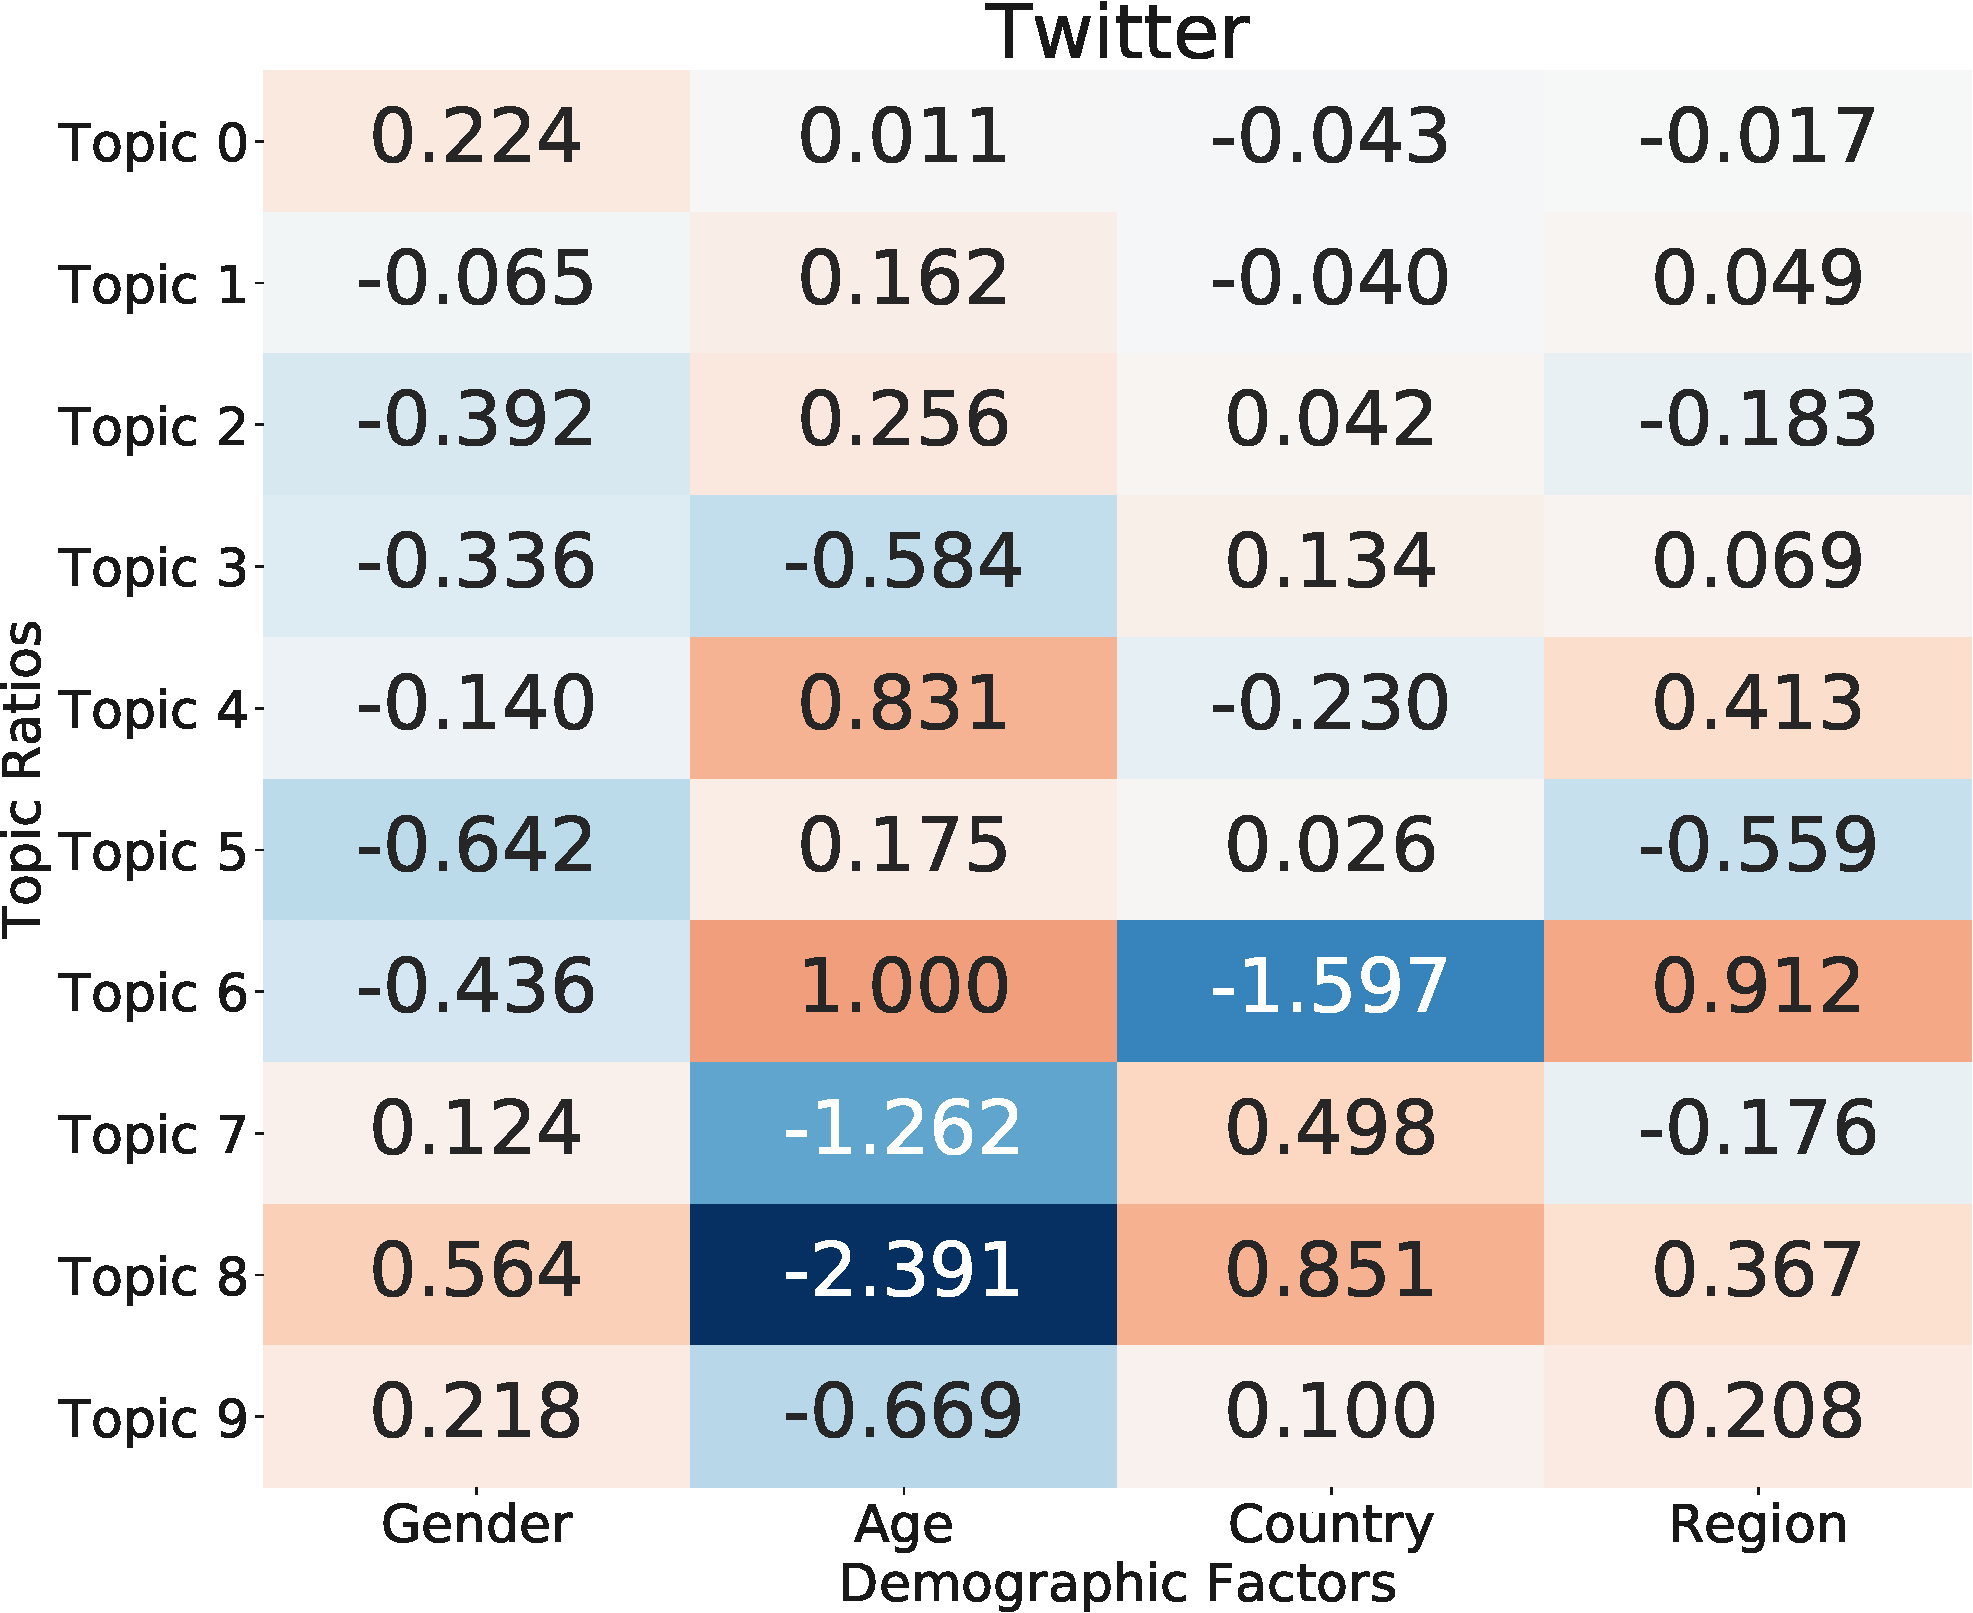
\includegraphics[width=0.44\textwidth]{./images/chapter4/twitter_ratio.pdf}
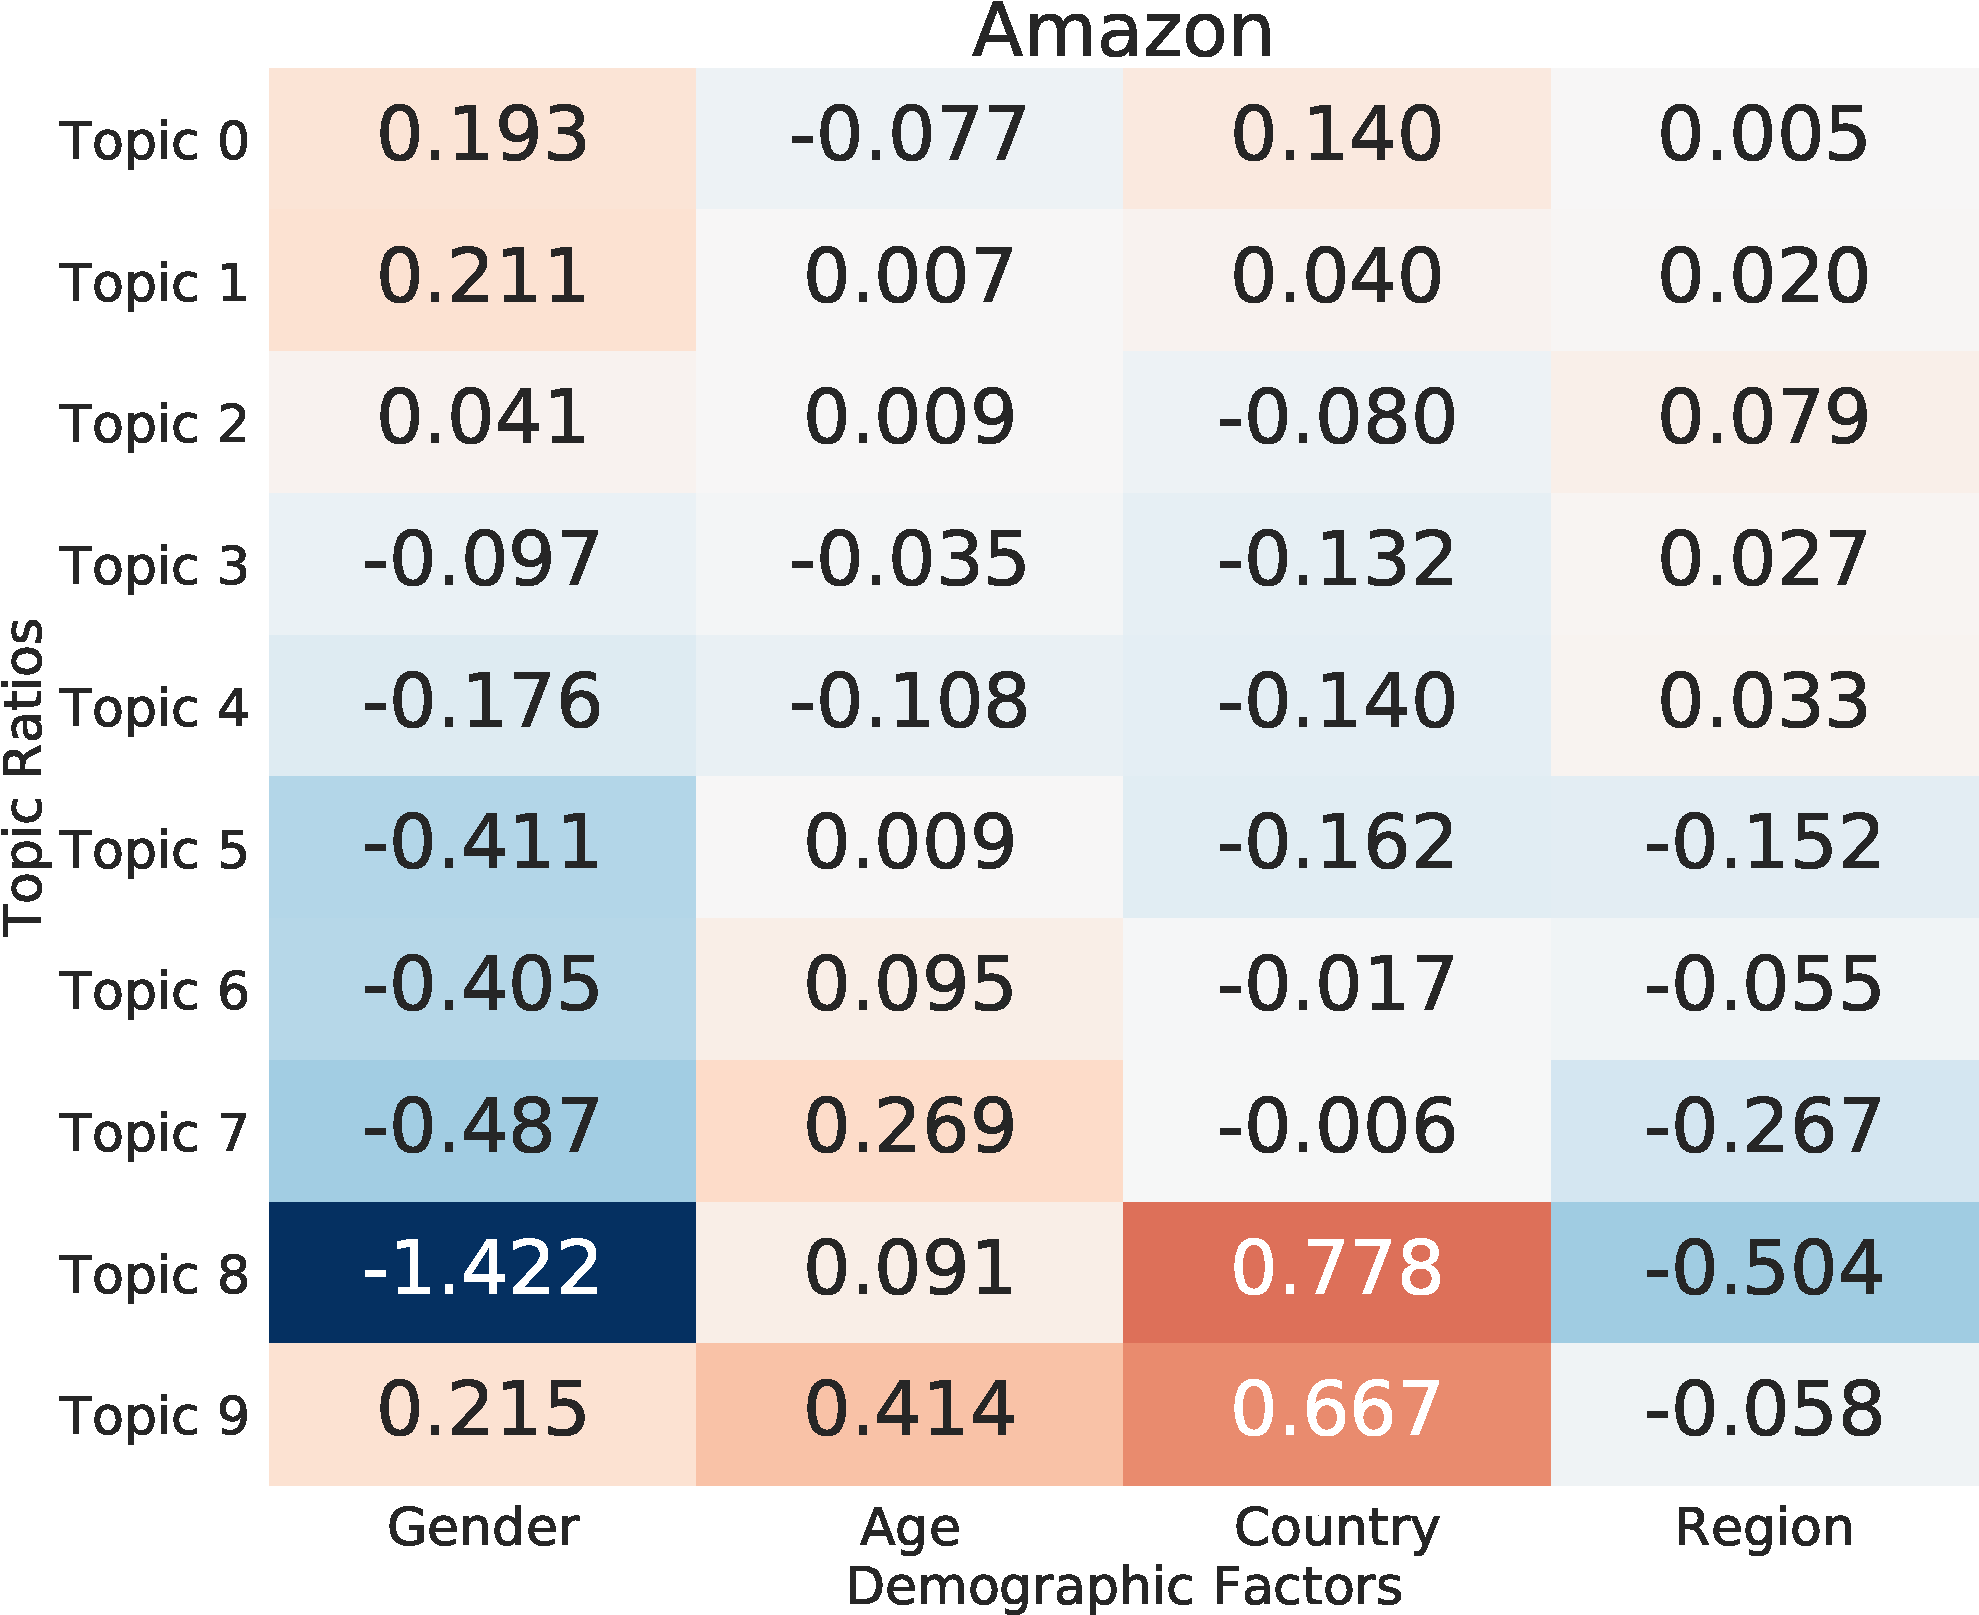
\includegraphics[width=0.44\textwidth]{./images/chapter4/amazon_ratio.pdf}
\newline
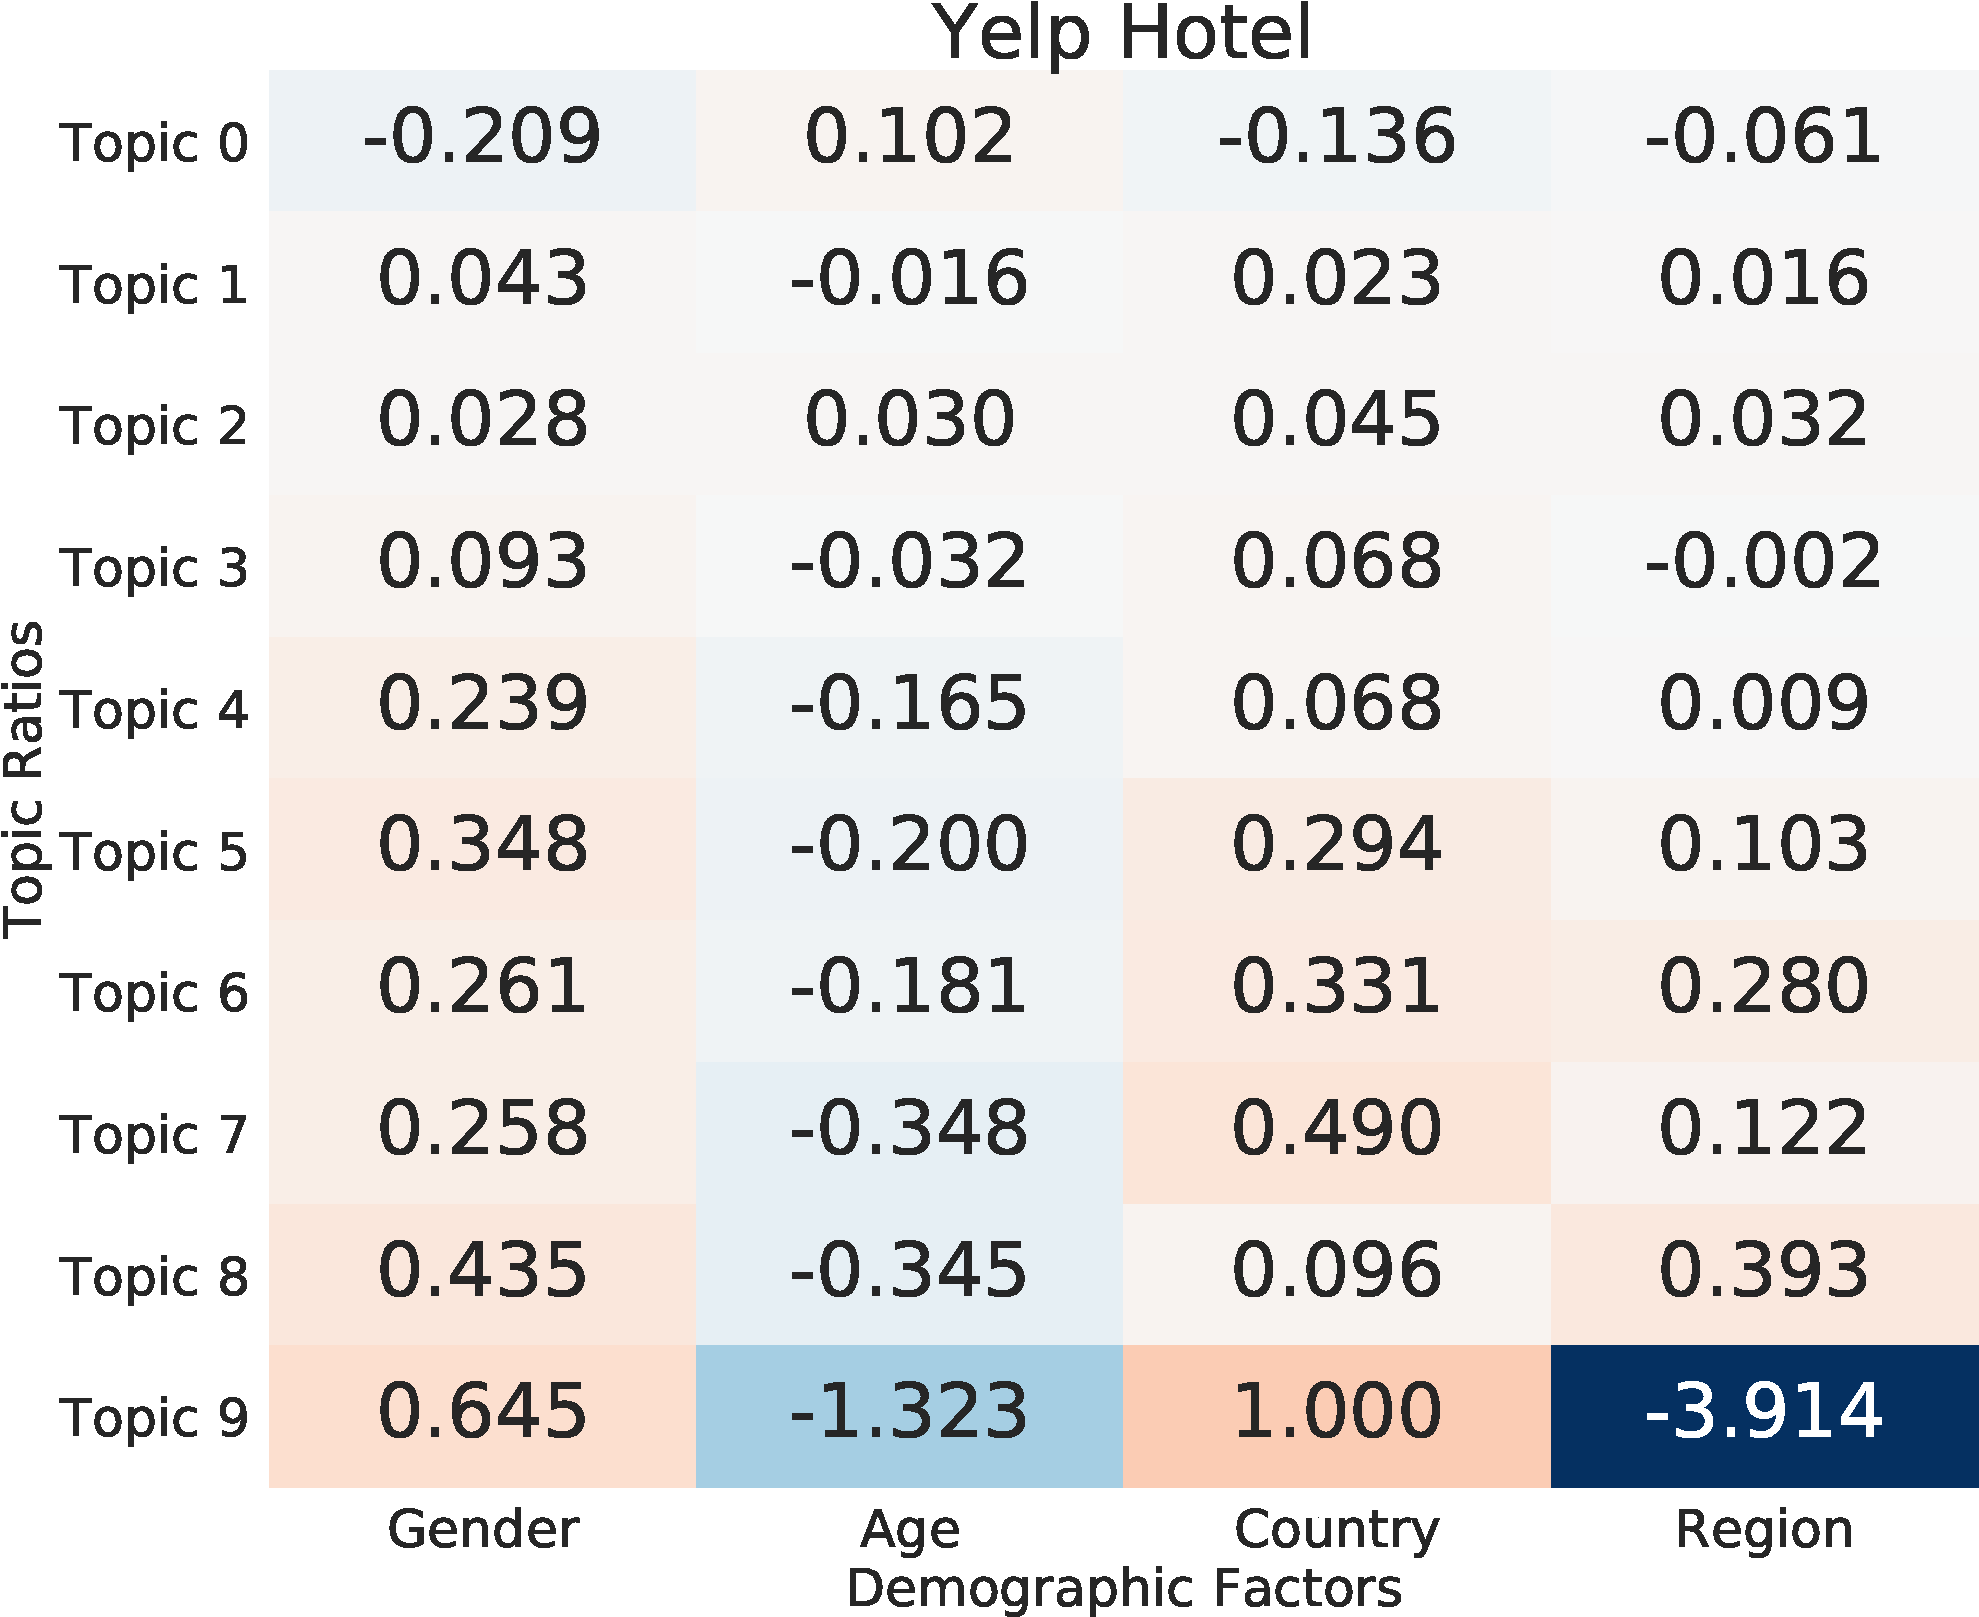
\includegraphics[width=0.44\textwidth]{./images/chapter4/yelp_hotel_ratio.pdf}
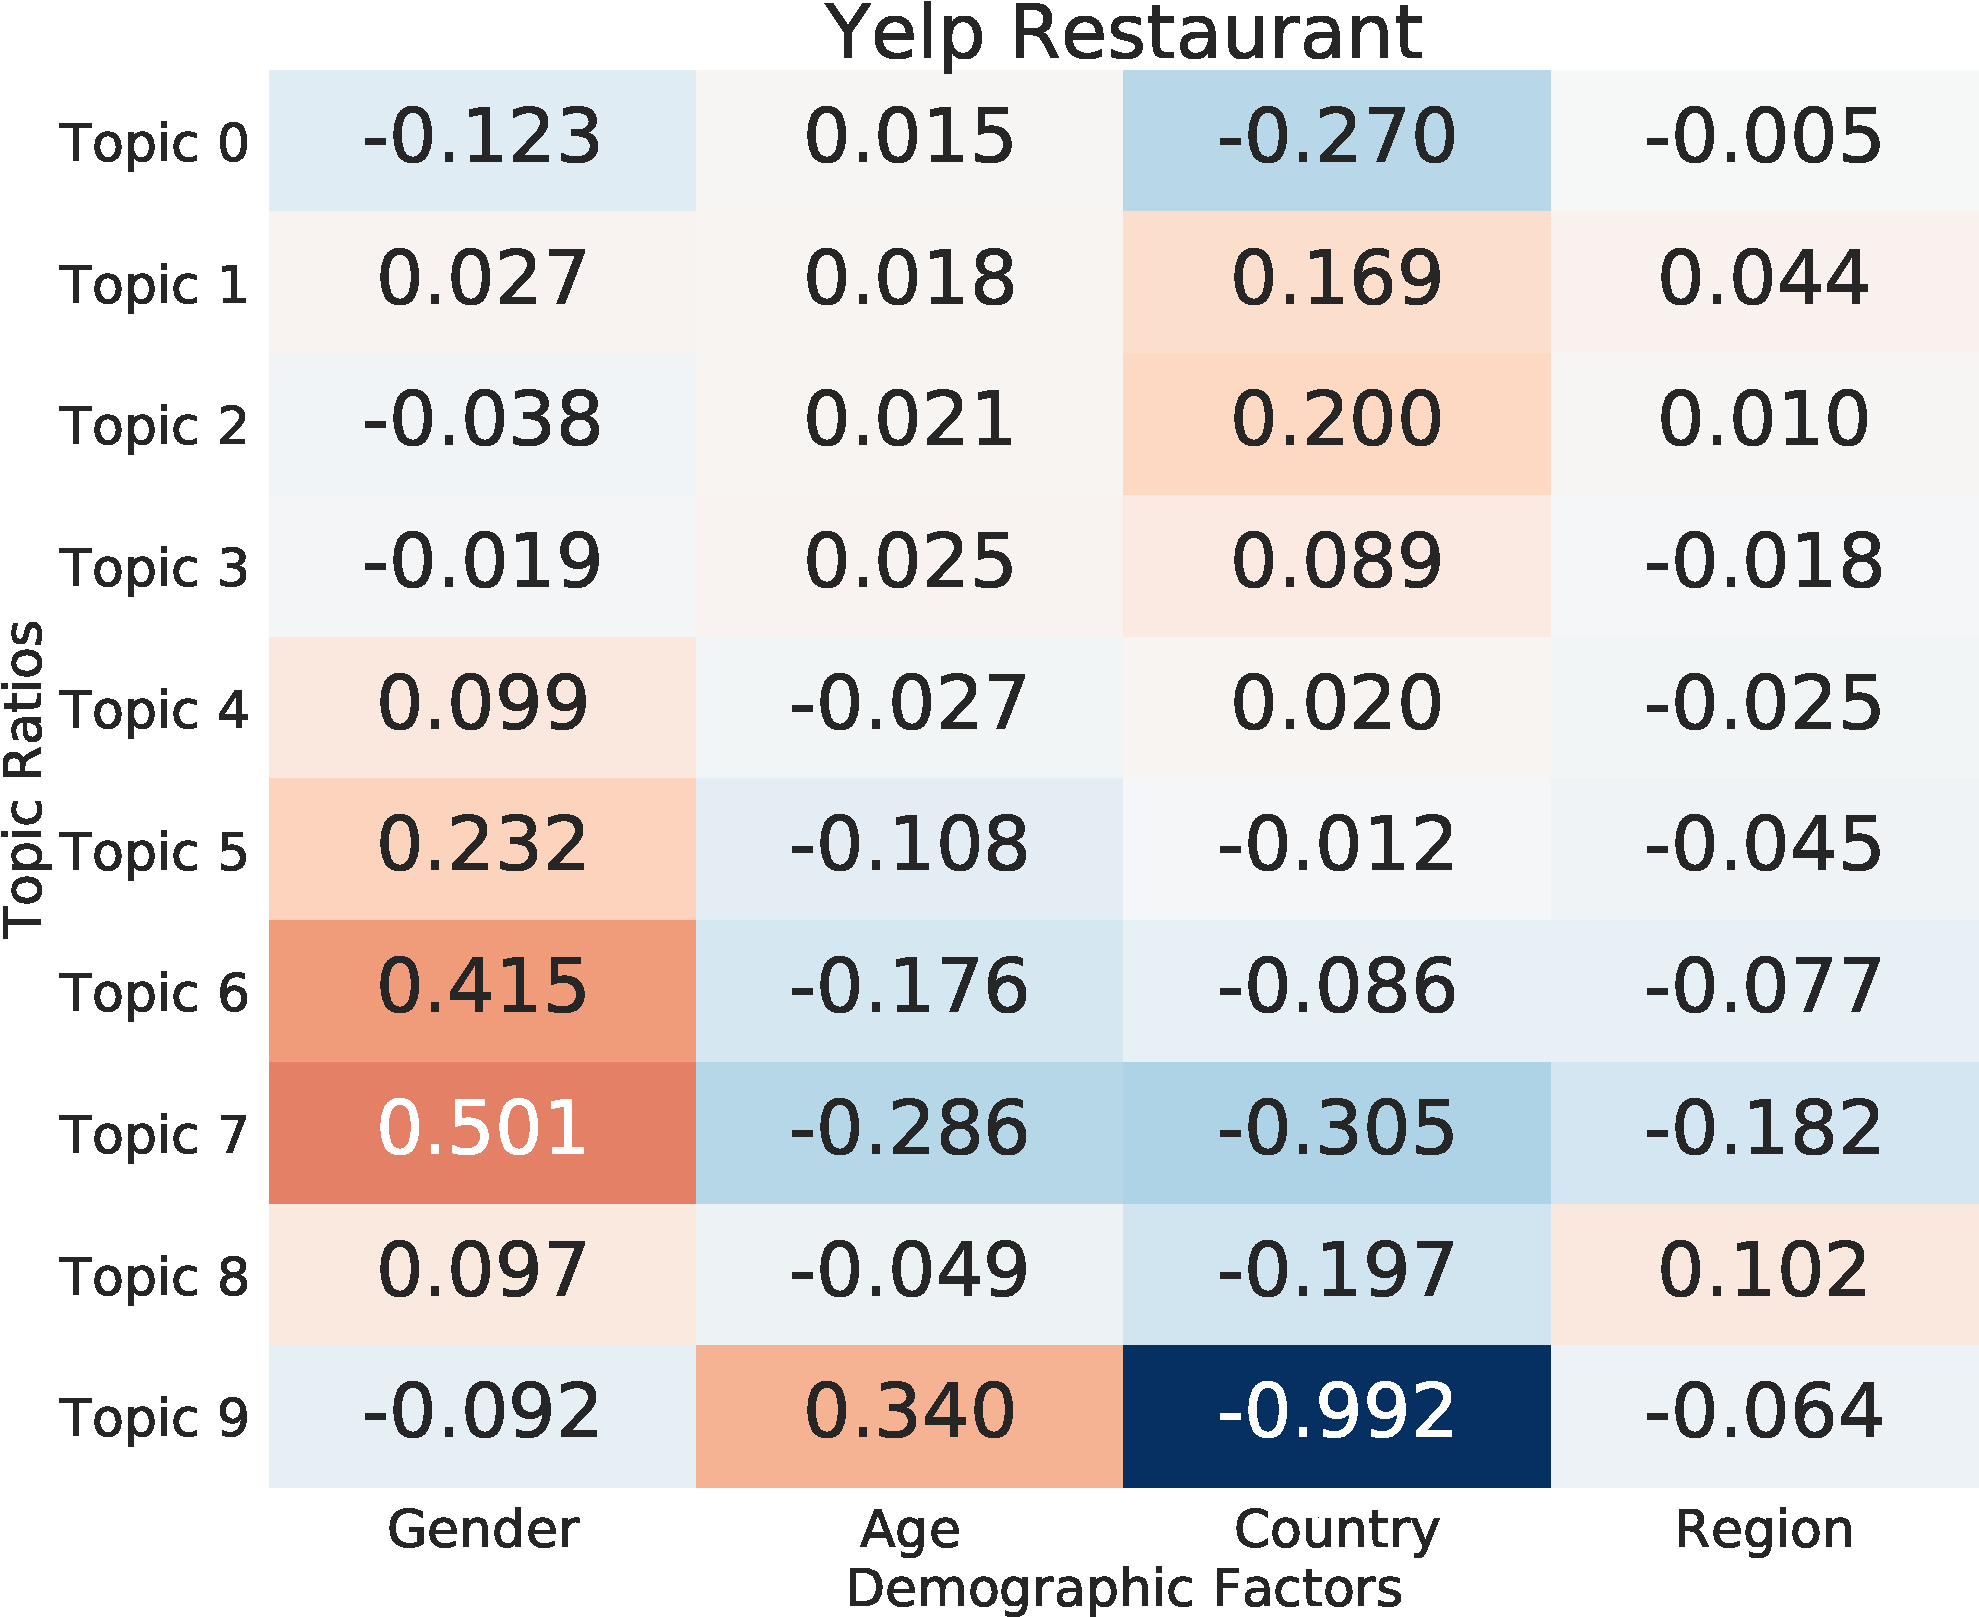
\includegraphics[width=0.44\textwidth]{./images/chapter4/yelp_rest_ratio.pdf}
\caption{Topic distribution log ratios. % for the Twitter, Amazon, Yelp Hotel and Yelp Restaurant data (from left to right) 
A value of 0 means that demographic groups use that topic in equal amounts, while values away from 0 mean that the topic is discussed more by one demographic group than the other group(s) in that factor.
}
\label{fig:vary}
\end{figure*}

We additionally examine how the distribution of text content varies across demographic groups. To characterize the content, we represent the text with a topic model.
We trained a Latent Dirichlet Allocation~\cite{blei2003latent} model with 10 topics using GenSim~\cite{rehurek2010software} with default parameters.
After training the topic model, each document $d$ is associated with a probability distribution over the 10 topics. 
The model learns a multinomial topic distribution $P(Z|D)$ from a Dirichlet prior, where $Z$ refers to each topic and $D$ refers to each document.
For each demographic group, we calculate the average topic distribution across the documents from that group.
Then within each factor, we calculate the log-ratio of the topic probabilities for each group.
For example, for topic $k$ for the gender factor,
we calculate $\log_2 \frac{P(Topic=k|Gender=\textrm{female})}{P(Topic=k|Gender=\textrm{male})}$.
The sign of the log-ratio indicates which demographic group is more likely to use the topic.
We do this for all factors;
for region, we simply binarize the four values for the purpose of this visualization (MW + W vs. NE + S).
Results are shown in Figure~\ref{fig:vary}.

%The model generates a multinomial topic distribution $P(Z|D)$ from a Dirichlet prior, where $Z$ is the topic distribution, and the D refers to documents. Particularly, we are interested in how the Z varies among gender ($P(Z|D, G)$), age ($P(Z|D, A)$), country ($P(Z|D, C)$) and region ($P(Z|D, R)$). We associated each document with one topic (the most likely topic in the document) and then calculated the proportion of each topic as the proportion of documents assigned to that topic. Next, to compare linguistic patterns, we calculate the ratios of each topic between types of the demographic factors: gender (female vs. male), age (young vs. old), country (US vs. no-US) and region (MW + W vs. NE + S). For example, we obtain male vs. female by $\frac{P(Z|D, female)}{P(Z|D, male)}$. Finally, we can visualize the extent to which the ratios of 10 topics varies by the four demographic attributes. We show the details in the Figure~\ref{fig:vary}.

The topic model was trained without removing stop words, in case stop word usage varies by group.
However, because of this, the topics all look very similar and are hard to interpret, so we do not show the topics themselves.
What we instead want to show is the degree to which the prevalence of some topics varies across demographic attributes, which are extracted independently from the text used to train the topic models.
We see that while most topics are fairly consistent across demographic groups, most datasets have at least a few topics with large differences.

%\cite{hovy2015demographic} show that demographic variations could associate with their linguistic behaviors online. To understand how linguistic behavior varies among the different demographic groups, we qualitatively examined and characterized how the distribution of content changes across the demographic attributes. 




%MP: Much of this text I included earlier, so now I am commenting it all out...


%\textbf{By gender} (G), $P(Z|D, G)$. Language styles highly associated with the gender of online users~\cite{hovy2018capturing}. The Figure~\ref{fig:vary} shows there are obvious variations between male (left stacked bar) and female (right stacked bar). The Twitter topic distributions are more on the first topic. We infer the reason might be the data is highly focused on ``flu vaccine''.
%

%\textbf{By age} (A), $P(Z|D, A)$. Some people change their linguistic styles as they age~\cite{wagner2012age}. We could partially confirm such a claim in our collected Twitter, Amazon and Yelp hotel data, which show more fluctuations of topic distributions. However, there are fewer variances in the Yelp restaurant data. 
%

%\textbf{By country} (C), $P(Z|D, C)$. From the third column of Figure~\ref{fig:vary}, we could observe that there are more significant variations in the Yelp restaurant data than other sources. It might be that people from different countries might express opinions in different ways. 
%

%\textbf{By region} (R), $P(Z|D, R)$. Goel et al.~\cite{goel2016social} show in online social media there are significantly different linguistic styles across different US regions. For example, due to English dialects among US regions, people in the Southern US use ``dese'' as ``these'' and people in Baltimore use ``ard'' as ``alright''. We might observe almost no variations in the Twitter data, which might be that people usually report ``flu vaccine'' in a similarly formal way. In contrast, we could observe that people talk more differently in the Amazon music data. 
%

\subsection{Are Document Categories Expressed Differently by Different User Groups?}

While text content varies across different user groups,
it is a separate question whether those variations will affect document classification.
For example, if men and women discuss different topics online,
but express sentiment in the same way,
then those differences will not affect a sentiment classifier.
Prior work has shown that the way 
people express opinions in online social media 
does vary by gender, age, geographic location, and political orientation~\cite{hinds2018demographic};
thus, there is reason to believe that concepts like sentiment will be expressed differently by different groups.
As a final exploratory experiment,
we now consider whether the text features that are predictive of
document categories (e.g., positive or negative sentiment)
also vary with user factors.

\begin{figure}[tb!]
\centering
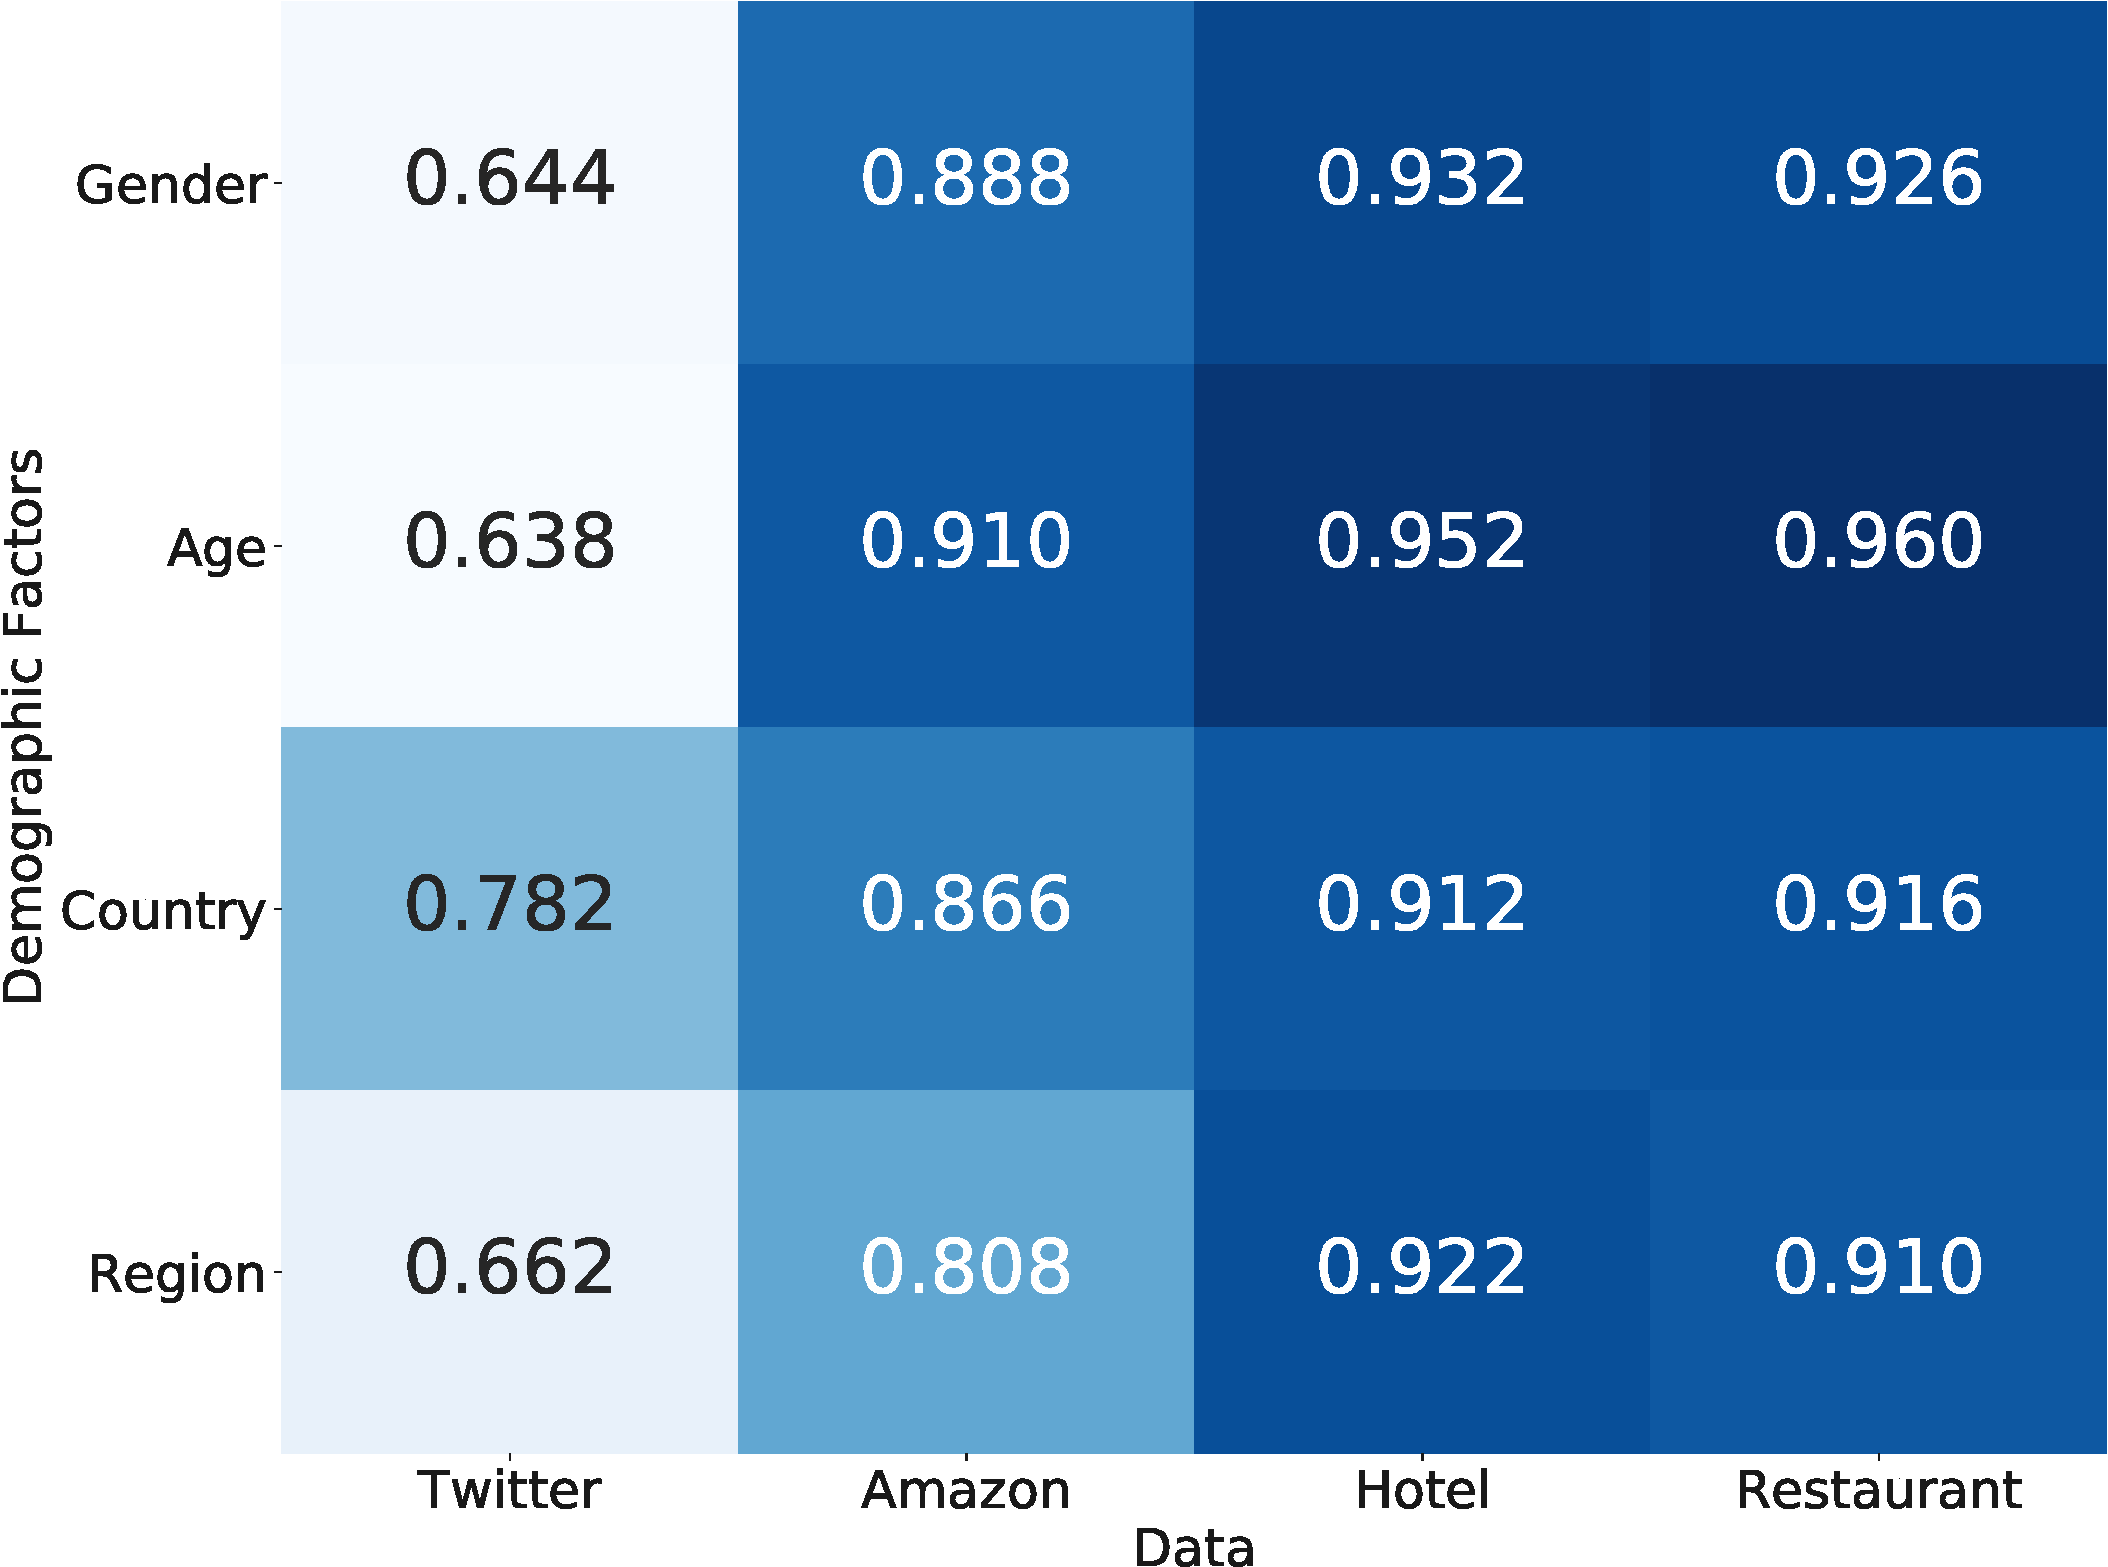
\includegraphics[scale=0.30]{./images/chapter4/overlap.pdf}
\caption{Overlap in most predictive classification features across different demographic groups, calculated for each demographic factor and each dataset. Darker color indicates less variation in word usage across demographic groups.
}
\label{fig:overlap}
\end{figure}

To compare how word expressions vary among the demographic factors, we conduct a word-level feature comparison.
For each demographic group, we collect only documents that belong to that group and then calculate the n-gram features (same features as in Section~\ref{subsec:analysis}) that are most associated with the document class labels.
Using mutual information, we select the top 1,000 features for each attribute.
Then within each demographic factor (e.g., gender),
we calculate the percentage of top 1,000 features that overlap across the different attribute values in that factor (e.g., male and female).
Specifically, if $S_0$ is the set of top features for one attribute and $S_1$ is the set of top features for another attribute, the percent overlap is calculated as $|S_0 \cap S_1|/1000$.
Results are shown in Figure~\ref{fig:overlap}. 
Lower percentages indicate higher variation in how different groups express the concepts being classified (e.g., sentiment).
The Twitter data shows the most variation while the Yelp hotel data shows the least variation.



\begin{figure*}[htp]
\centering
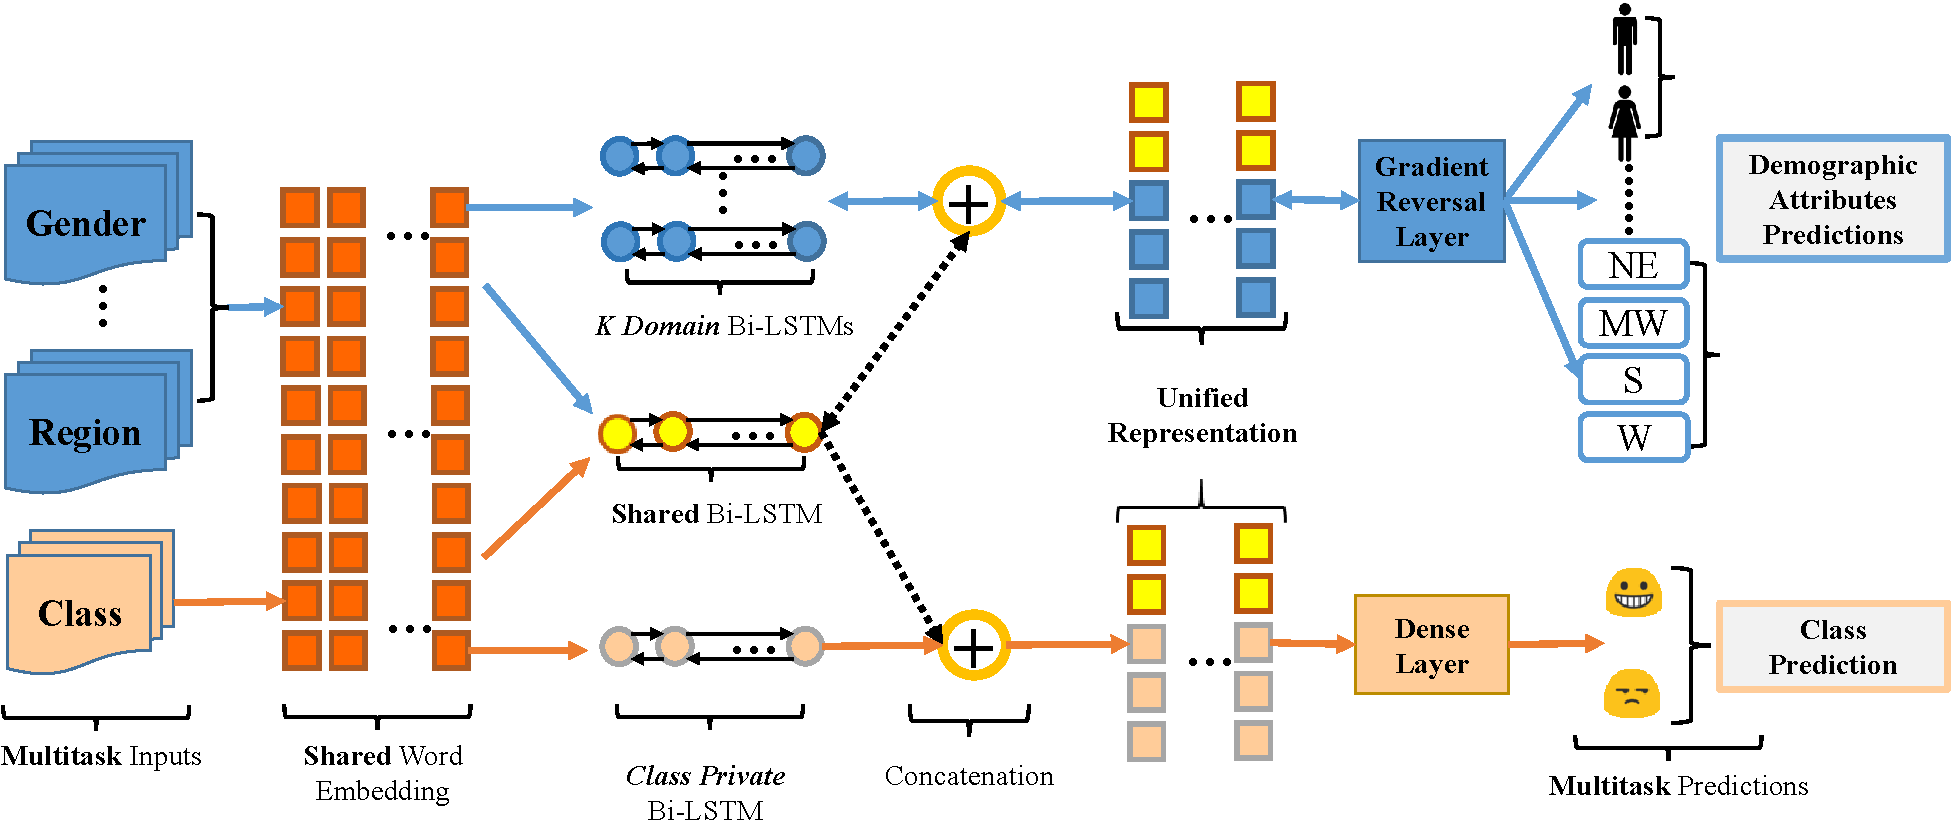
\includegraphics[scale=0.47]{./images/chapter4/model.pdf}
\caption{Neural User Factor Adaptation (NUFA) model. 
%``Class'' refers to the class labels of the documents, which are binary-valued. 
NUFA optimizes for two major tasks, demographic prediction (blue blocks and arrows) and text classification (light orange blocks and arrows). 
During the training phase, documents labeled with demographic information go through the demographic classifier, and documents with class labels go through the document classifier. 
This helps NUFA learn representations that are useful for classifying documents versus representations that are useful for predicting demographics.
At test time, documents are given only to the document classifier, leaving out the demographic classifiers. 
%In this way, NUFA could adapt user demographic knowledge into the text classifier.
}
\label{fig:model}
\end{figure*}

\subsection{Model}
\label{sec:model}

Models for user factor adaptation generally treat
this as a problem of {\em domain adaptation}~\cite{volkova2013exploring,lynn2017human}.
Domain adaptation methods are used to learn models that can be applied to data whose distributions may differ from the training data.
Commonly used methods include feature augmentation~\cite{daume2007frustratingly, joshi2013s, huang2018examining}
and structural correspondence learning~\cite{blitzer2006domain},
while recent approaches rely on 
domain adversarial training~\cite{ganin2016domain, chen2016adversarial, liu2017adversarial, huang2018modeling}. 
We borrow concepts of domain adaptation to construct a model that is robust to variations across user factors.


In our proposed {\bf Neural User Factor Adaptation (NUFA)} model, we treat each variable of interest (demographic attributes and document class label) as a separate, but jointly modeled, prediction task.
%additionally, we treat each demographic attribute as a domain for the purpose of adaptation. 
The goal is to perform well at predicting document classes, while the demographic attribute tasks are modeled primarily for the purpose of learning characteristics of the demographic groups.
%Our primary goal is to learn to account for user demographic information in a way that improves the performance of the document classification model. 
Thus, the model aims to learn discriminative features for text classification while learning to be invariant to the linguistic characteristics of the demographic groups. 
Once trained, this classifier can be applied to test documents without requiring the demographic attributes.

Concretely, we propose the multitask learning framework in Figure~\ref{fig:model}. 
The model extracts features from the text for the demographic attribute prediction tasks and the classification task, as well as joint features for all tasks in which features for both demographics and document classes are mapped into the same vector space.
%\textcolor{red}{We employ a shared embedding feature extractor to map both features from demographic attributes and document classes into the same vector space, which aims to keep the model from being distracted by different input sources.}
Each feature space is constructed with a separate Bidirectional Long Short-Term Memory model (Bi-LSTM)~\cite{hochreiter1997long}.

Because language styles vary across groups, as shown in Section~\ref{subsec:analysis}, information from each task could be useful to the other.
Thus, our intuition is that while we model the document and demographic predictions as independent tasks, the shared feature space allows the model to transfer knowledge from the demographic tasks to the text classification task and vice versa. 

However, we want to keep the feature space such that
the features are predictive of document classes in a way that is invariant to demographic shifts. 
To avoid learning features for the document classifier that are too strongly associated with user factors, 
we use adversarial training.
The result is that the demographic information is encoded primarily in the features used for the demographic classifiers, while learning invariant text features that work {\em across} different demographic groups for the document classifier. 

%\vspace{-1ex}
\paragraph{Domain Sampling and Model Inputs.} 
Our model requires all domains (demographic attributes) to be known during training, but not all attributes are known in our datasets.
Instead of explicitly modeling the missing data,
we simply sample documents where all user attributes of interest are available.
At test time, this limitation does not apply because only the document text is required as input to the document classifier.

%We feed the inputs with all text documents. However, one issue with user demographic label in the real world is ``missing labels'', for example, a user might not provide any private information. Moreover, we could not do the same training steps that proposed in the previous research~\cite{chen2016adversarial} that treats sampled training data as positive and test data as negative. Because they do not have ``missing labels'' issue and in our scenario, demographic labels are well uniformly distributed in both training and test data. Therefore, we sample a batch of documents that have labels for each demographic prediction task. Noted that we only feed data to the document classifier during the test stage.

%\vspace{-1ex}
\paragraph{Shared Embedding Space.} We use a common embedding layer for both document and demographic factor predictions. The goal is that the trained embeddings will capture the language variations that are associated with the demographic groups as well as document labels. Parameters are initialized with pre-trained  embeddings~\cite{mikolov2013distributed, pennington2014glove}.

%\vspace{-1ex}
\paragraph{K+2 Bi-LSTMs.} We combine ideas from two previous works on domain adaptation~\cite{liu2017adversarial, kim2017domain}. Kim et al.~\cite{kim2017domain} proposed $K$$+$$1$ Bi-LSTMs, where $K$ is the number of domains, and Liu et al.~\cite{liu2017adversarial} proposed to combine shared and independent Bi-LSTMs for each prediction task. In our model, we create one independent Bi-LSTM for each demographic domain (blue), one independent Bi-LSTM for the document classifier (orange), and one shared Bi-LSTM that is used in both the demographic prediction and document classification tasks (yellow). The intuition is to transfer learned information to one and the other through this shared Bi-LSTM while leaving some free spaces for both document label and demographic factors predictions. We then concatenate outputs of the shared LSTM with each task-independent LSTM together. This helps the text classifier capture demographic knowledge.

%\vspace{-1ex}
\paragraph{Demographic Classifier.} 
We adjust the degree to which the demographic classifiers can discriminate between attributes. 
To find a balance between the invariant knowledge and differences across user demographic factors, we apply domain adversarial training~\cite{ganin2016domain} (the blue block indicating the ``gradient reversal layer'') to each domain prediction task. The predictions use the final concatenated representations, where the prediction is modeled with a {softmax} function for the region and a binary {sigmoid} function for the other user demographic factors. 

%\vspace{-1ex}
\paragraph{Document Classifier.} We feed the concatenated outputs of the document and shared Bi-LSTMs to one layer feed-forward network (the orange block indicating the ``dense layer''). Finally, the document classifier outputs a probability via a sigmoid.

%\vspace{-1ex}
\paragraph{Joint Multitask Learning.} We use the categorical cross-entropy loss to optimize the $K+1$ prediction tasks jointly. One question is how to assign importance to the multiple tasks. Because our target is document classification, we assign a cost to the domain prediction loss ($L_{domain}$). Each prediction task has its own weight, $\alpha_k$. The final loss function is defined as $L = L_{doc} + \sum_{k=1}^K \alpha_k L_{domain, k}$. In summary, the proposed model learns and adapts to user demographic factors through three aspects: shared embeddings, shared Bi-LSTMs, and joint optimization.

\subsection{Experiments}
\label{sec:experiments}
  
We experiment with document classification on our four corpora using various models. Our goal is to test whether models that adapt to user factors can outperform models that do not, and to understand which components of models can facilitate user factor adaptation.
  
\subsubsection{Data Processing}

We replaced hyperlinks, usernames, and hashtags with generic symbols. Documents were lowercased and tokenized using NLTK~\cite{bird2004nltk}. 
The corpora were randomly split into training (80\%), development (10\%), and test (10\%) sets. %, summarized in Table~\ref{table:statics}. 
We train the models on the training set and find the optimal hyperparameters on the development set. We randomly shuffle the training data at the beginning of each training epoch. The evaluation metric is weighted F1 score.

%%MP: This table isn't needed, because you can get the same information from the earlier data table in section 2, and the fact that the data split is 80/10/10.
%
%\begin{table}[ht]
%  \centering
%  \resizebox{\columnwidth}{!}{
%    \begin{tabular}{c|ccc|c}
%     \hline\hline
%     Datasets & Train & Dev. & Test & Total\\
%     \hline
%     Twitter & 7,875 & 984 & 985 & 9,844 \\
%     Amazon & 32,335 & 4,042 & 4,042 & 40,419 \\
%     Hotel & 135,164 & 16,896 & 16,896 & 168,956 \\
%     Restaurant & 570,750 & 71,344 & 71,344 & 713,438 \\
%     \hline
%    \end{tabular}
%    }
%    \caption{Data statistics.}
%    \label{table:statics}
%\end{table}
%
%%

\subsubsection{No Adaptation Baselines}
We compare to three standard classifiers that do not perform adaptation.


%\vspace{-.5ex}
\paragraph{N-gram.} We extract TF-IDF-weighted features of 1-, 2-, and 3-grams on the corpora, using the most frequent 15K features with the minimum feature frequency as 2.
We trained a logistic regression classifier using the \texttt{SGDClassifier} implementation in scikit-learn~\cite{pedregosa2011scikit}
using a batch size of 256 and 1,000 iterations. 

%\vspace{-.5ex}
\paragraph{CNN.} We used Keras~\cite{chollet2015keras} to implement the Convolutional Neural Network (CNN) classifier described in~\cite{kim2014convolutional}. To keep consistent, we initialize the embedding weight with pre-trained word embeddings~\cite{mikolov2013distributed,pennington2014glove}. We only keep the 15K most frequent words and replace the rest with an ``unk'' token. Each document was padded to a length of 50. We keep all parameter settings as described in the paper. We fed 50 documents to the model each batch and trained for 20 epochs.

%\vspace{-.5ex}
\paragraph{Bi-LSTM.} We build a bi-directional Long Short Term Memory (bi-LSTM)~\cite{hochreiter1997long} classifier. The classifier is initialized with the pre-trained word embeddings, and we initialize training with the same parameters used for the NUFA.



\subsubsection{Adaptation Models}

We consider two baseline domain adaptation models that can adapt for user factors, a non-neural method and a neural model.
We then provide the training details of our proposed model, NUFA.
Finally, we consider two variants of NUFA that ablate components of the model, allowing us to evaluate the contribution of each component.

%\vspace{-.5ex}
\paragraph{FEDA.} Lynn et al.~\cite{lynn2017human} used a modification of the ``frustratingly easy'' domain adaptation (FEDA) method~\cite{daume2007frustratingly} to adapt for user factors. 
We use a modification of this method where the four user factors and their values are treated as domains.
We first extract domain-specific and general representations as TF-IDF-weighted n-gram (1-, 2, 3-grams) features. We extract the top 15K features for each domain and the general feature set.
With this method, the feature set is augmented such that each feature has a domain-specific version of the feature for each domain, as well as a general domain-independent version of the feature.
%MP: Cutting these details/examples to save space
%for a total of $1+\sum_{k=1}^{K}C_k$ feature sets, where $C_k$ is the number of categories for the $k$th domain. 
The features values are set to the original feature values for the domain-independent features and the domain-specific features that apply to the document, while domain-specific features for documents that do not belong to that domain are set to $0$.
For example, using gender as a domain, a training document with a female author would be encoded as $[F_{general}, F_{domain, female}, 0]$, while a document with a male author would be encoded as $[F_{general}, 0, F_{domain, male}]$.
Different from prior work with FEDA for user-factor adaptation, 
at test time we only use the general, domain-independent features;
the idea is to learn a generalized feature set that is domain invariant.
This is the same approach we used in recent work using FEDA to adapt classifiers to temporal variations~\cite{huang2018examining}.



%\vspace{-.5ex}
\paragraph{DANN.} We consider the domain adversarial training network~\cite{ganin2016domain} (DANN) on the user factor adaptation task. We use Keras to implement the same network and deploy the same pre-trained word embeddings as in NUFA. We then set the domain prediction as the demographic factors prediction and keep the document label prediction as the default. We train the model with 20 epochs with a batch size of 64. Finally, we use the model at the epoch when the model achieves the best result on the development set for the final model.


%\vspace{-0.5ex}
\paragraph{NUFA.}
We initialize the embedding weights by the pre-trained word embeddings~\cite{mikolov2013distributed, pennington2014glove} with 200 dimensional vectors. All LSTMs are fixed outputs as 200-dimension vectors. We set the dropout of LSTM training to 0.2 and the flip gradient value to .01 during the adversarial training. The dense layer has 128 neurons with ReLU activation function and dropout of 0.2. User factors and document label predictions are optimized jointly using Adam~\cite{kingma2014adam} with a learning rate of 0.001 and batch size of 64. We train NUFA for up to 20 epochs and select the best model on the development set. 
For single-factor adaptation (next section), we set $\alpha$ to 0.1;
for multi-factor adaptation, we use a heuristic for setting $\alpha$ described in that section.
We implemented NUFA in Keras~\cite{chollet2015keras}.

%\vspace{-0.5ex}
\paragraph{NUFA--s.} To understand the role of the shared Bi-LSTM in our model, we conduct experiments on NUFA without the shared Bi-LSTM. We follow the same experimental steps as NUFA and denote it as NUFA$-$s (NUFA minus shared Bi-LSTM). %\textcolor{red}{This will enforce separated training process of the prediction tasks and directly impacts the shared embedding layer.}

%\vspace{-0.5ex}
\paragraph{NUFA--a.} To understand the role of the adversarial training in our model, we conduct experiments of the NUFA without adversarial training, denoted as NUFA$-$a (NUFA minus adversarial).



\begin{table}[tb!]
\centering
\begin{tabular}{c|c|c|c|c}
 & Twitter & Amazon & Hotel & Rest. \\\hline
 \multicolumn{5}{c}{No Adaptation} \\\hline
N-gram & .866 & .793 & .857 & .866 \\
CNN & .879 & .776 & .825 & .846 \\
Bi-LSTM & .869 & .776 & .842 & .875 \\\hline
\multicolumn{5}{c}{Adaptation (Gender)} \\\hline
FEDA & .814 & .809 & \textbf{.865} & .874 \\
DANN & .864 & .832 & .813 & .855 \\ \hline
NUFA$-$s & .880 & \em .845 & .857 & .869 \\
NUFA$-$a & .874 & .842 & .852 & .868 \\
NUFA & \em .886 & .844 & .854 & \textbf{.881} \\ \hline
\multicolumn{5}{c}{Adaptation (Age)} \\\hline
FEDA & .813 & .801 & \bf .865 & .873 \\
DANN & .856 & .824 & .811 & .851 \\ \hline
NUFA$-$s & .872 & \em .843 & .850 & .879 \\
NUFA$-$a & .882 & .841 & .852 & .878 \\
NUFA & \em .885 & .839 & .857 & \em .880 \\ \hline
\multicolumn{5}{c}{Adaptation (Country)} \\\hline
FEDA & .826 & .768 & \bf .865 & .877 \\
DANN & .868 & .828 & .827 & .855 \\ \hline
NUFA$-$s & .882 & \em .844 & .854 & \em .879 \\
NUFA$-$a & .880 & .838 & .855 & .877 \\
NUFA & \textbf{.896} & .843 & .854 & \em .879 \\ \hline
\multicolumn{5}{c}{Adaptation (Region)} \\\hline
FEDA & .826 & .780 & \em .864 & .869 \\
DANN & .875 & .825 & .823 & .852 \\\hline
NUFA$-$s & .874 & .833 & .854 & .878 \\
NUFA$-$a & .882 & .838 & .854 & .875 \\
NUFA & \em .893 & \textbf{.848} & .853 & \em .880\\ \hline
\end{tabular}
\caption{Performance (weighted F1) of no adaptation and single user factor adaptation.
For each dataset, the best score within each demographic domain is italicized; the best score overall is bolded.
}
\label{table:single}
\end{table}

\subsubsection{Results}

\paragraph{Single-Factor Adaptation.} We first consider user factor adaptation for each of the four factors individually. 
Table~\ref{table:single} shows the results.
Adaptation methods almost always outperform the non-adaptation baselines;
the best adaptation model outperforms the best non-adaptation model by $1.5$ to $5.5$ points. 
The improvements indicate that adopting the demographic factors might be beneficial for the classifiers. User factor adaptation thus appears to be important for text classification. 

Comparing the adaptation methods,
our proposed model (NUFA) is best on three of four datasets.
%The Table~\ref{table:single} also shows that our proposed mode with the best result usually outperforms other baselines and particularly exceeds the neural model baseline (DANN) on all datasets. The results show our neural learning framework could effectively learn and adapt the demographic differences into the text classification task. 
On the Hotel dataset, the n-gram model FEDA is always best;
this seems to be a dataset where neural methods perform poorly, since even the n-gram baseline with no adaptation often outperformed the various neural models. 
Whether a neural model is the best choice depends on the dataset,
but among the neural models, NUFA always outperforms DANN.
Finally, the full NUFA model most often outperforms the variants without the shared Bi-LSTM (NUFA$-$s) and without adversarial training (NUFA$-$a). 


\paragraph{Multi-Factor Adaptation.} We experiment with adapting to all four user factors together.
Recall that each domain prediction task in NUFA is weighted by $\alpha_k$.
Initially, we simply used a uniform weighting, $\alpha_k = \alpha/K$,
but we find that we can improve performance with non-uniform weighting.
Because optimizing the $\alpha$ vector would be expensive, 
we instead propose a heuristic that weighs the domains
based on how much each domain is expected to influence the text.
We define $\alpha_k = s_k / (\sum_{k'} s_{k'})$, where $s_k$ is the F1 score of demographic attribute prediction for domain $k$ from Table~\ref{table:explo}.
We denote this method as {\bf NUFA+w}, which refers to this additional weighting process.

\begin{table}[t]
\centering
\begin{tabular}{c|c|c|c|c}
 & Twitter & Amazon & Hotel & Rest. \\\hline
\multicolumn{5}{c}{Baseline Adaptation} \\\hline
FEDA & .806 & .778 & \bf .867 & .869 \\\hline
DANN & .880 & .828 & .830 & .858 \\\hline
\multicolumn{5}{c}{Proposed Model} \\\hline
NUFA & .887 & .848 & .853 & .879 \\
NUFA+w & \bf .901 & \bf .852 & .855 & \bf .885 \\
\end{tabular}
%\vspace{-1ex}
\caption{Results of adaptation for all four user factors.}
\label{table:multi}
\end{table}

Table~\ref{table:multi} shows that combining all user factors
provides a small gain over single-factor adaptation;
the best multi-factor result is higher than the best single-factor result for each dataset.
As with single-factor adaptation, FEDA works best for the Hotel datasets,
while NUFA+w works best for the other three.
Without adding weighting to NUFA, the multi-factor performance is comparable to single-factor performance;
thus, task weighting seems to be critical for good performance when combining multiple factors.



%In this paper, we view the modeling demographic factors as a domain adaptation problem. We integrate the demographic attributes into our text classification model via multitask learning framework.

%MP: I think the background on DA and user factors should probably just be incorporated earlier in the paper when these are first introduced. I can work on doing that when I edit sections 1-2 later.
%XL: I see. I put the related works here because I thought we covered the partially related works in the introduction and the section might not be as important as our proposed method. 

%\textbf{Domain adaptation} tries aligning source with related target distributions to obtain more generalized feature representations and classifiers. For the text classification task, there are two conventional methods, feature augmentations~\cite{daume2007frustratingly, blitzer2006domain, huang2018examining} and domain adversarial training~\cite{ganin2016domain, chen2016adversarial, liu2017adversarial}. However, one issue with the proposed methods is they did not consider the user demographic factors, which show strong variations among social media documents. Additionally, most of the adaptation only work on two different domains, but the demographic factors have more complex domains and divergent differences between domains.

%\textbf{User factor adaptation} integrates demographic factors into the machine learning classifiers. The demographic factors usually refer to the attributes of users, such as gender, age, geographic location, etc. Online generated user texts show demographic variations in the linguistic styles, and the linguistic style differences could be used for the use factor prediction~\cite{rosenthal2011age, zhang2016predicting, hovy2018improving}. The user factors impact on how online users express their opinions and show promising improvements in the text classification task~\cite{volkova2013exploring, hovy2015demographic, lynn2017human, yang2017overcoming}. The closest work to our study~\cite{lynn2017human} created general and domain-specific features to train a more generalized classification model. However, such a method heavily suffers extremely high feature dimensions and handcraft features. 


\section{User Factor Adaptation via User Embedding}

\subsection{Data}

\subsection{Multitask Learning Framework}

\subsection{Experiments}

\subsubsection{User Embedding Evaluation}

\begin{table*}[htp]
\centering
\resizebox{\textwidth}{!}{
    \begin{tabular}{cc||ccc|ccc|ccc}
    \multicolumn{2}{c||}{\multirow{2}{*}{}} & \multicolumn{3}{c|}{Amazon-Health} & \multicolumn{3}{c|}{IMDB} & \multicolumn{3}{c}{Yelp} \\
    \multicolumn{2}{c||}{} & F1@4 & F1@8 & F1@12 & F1@4 & F1@8 & F1@12 & F1@4 & F1@8 & F1@12 \\\hline\hline
    \multirow{5}{*}{Baselines} & word2user &  &  &  &  &  &  &  &  &  \\
     & lda2user &  &  &  &  &  &  &  &  &  \\
     & doc2user &  &  &  &  &  &  &  &  &  \\
     & bert2user &  &  &  &  &  &  &  &  &  \\
     & user2vec &  &  &  &  &  &  &  &  &  \\\hline
    \multirow{3}{*}{Ours} & MTL-global &  &  &  &  &  &  &  &  &  \\
     & MTL-decay &  &  &  &  &  &  &  &  &  \\
     & MTL-local &  &  &  &  &  &  &  &  & 
    \end{tabular}
}
\caption{}
\label{chap4:tab:usereval}
\end{table*}


\subsubsection{Classifier Personalization}


\begin{table*}[htp]
\centering
\begin{tabular}{c||ccc|ccc|ccc}
\multirow{2}{*}{Methods} & \multicolumn{3}{c|}{Amazon-Health} & \multicolumn{3}{c|}{IMDB} & \multicolumn{3}{c}{Yelp} \\
 & Precision & Recall & F1 & Precision & Recall & F1 & Precision & Recall & F1 \\\hline\hline
LR & .834 & .768 & .793 & .818 & .779 & .794 & .856 & .820 & .833 \\
LR-p & .838 & .771 & .796 & .833 & .790 & .807 & .863 & .825 & .838 \\\hline
GRU & .813 & .844 & .812 & .824 & .837 & .823 & .851 & .865 & .852 \\
GRU-p & .821 & .832 & .825 & .838 & .804 & .819 & .867 & .860 & .863 \\\hline
BERT & .866 & .822 & .840 & .852 & .809 & .826 & .866 & .825 & .840 \\
BERT-p &  &  &  &  &  &  &  &  & 
\end{tabular}
\caption{}
\label{chap4:tab:personalization}
\end{table*}

\section{Conclusion}

We have explored the issue of author demographics in relation to document classification,
showing that demographics are encoded in language, and the most predictive features for document classification vary by demographics.
We showed that various domain adaptation methods can be used to build classifiers that are more robust to demographics, combined in a neural model that outperformed prior approaches.
While our work is not focused specifically on reducing bias,
our goals are related to it in that our models are meant to learn document classifiers that are invariant to author demographics.
Our datasets, which contain various attributes including those inferred through facial recognition, could be useful in other research (Chapter~\ref{chap2:sec:demographic}). We publish our datasets\footnote{\url{http://cmci.colorado.edu/~mpaul/files/starsem2019_demographics.data.zip}} and source code.\footnote{\url{https://github.com/xiaoleihuang/NUFA}}
\chapter{NLP Ethics and Fairness}
\label{chp:fairness}

\section{Introduction}

% Recent research raises concerns that document classification models can be discriminatory and can perpetuate human biases~\cite{dixon2018measuring,kiritchenko2018examining,park2018reducing,garg2019counterfactual,borkan2019nuanced}.
% \textit{Fairness}-aware classifiers aim to provide fair, non-discriminatory outcomes towards people or groups of people based on their demographic attributes, such as gender or race. 
% Fairness has been defined in different ways~\cite{hardt2016equality};
% for the document classification task, existing research~\cite{dixon2018measuring,kiritchenko2018examining,park2018reducing,garg2019counterfactual,heindorf2019debiasing} has focused on \textit{group fairness}~\cite{chouldechova2018frontiers}, under which document classifiers are defined as biased if the \textit{classifiers perform better for documents of some groups than for documents of other groups}.


% However, fairness of document classifiers has only been evaluated based on the token level instead of the author level~\cite{kiritchenko2018examining,dixon2018measuring,park2018reducing,heindorf2019debiasing,davidson2019racial,sun2019mitigating}, because the public corpora do not contain demographic variables of the users~\cite{blodgett2016demographic,wulczyn2017ex,kiritchenko2018examining}.
% For example, the Wikipedia Talk corpus\footnote{\url{https://figshare.com/articles/Wikipedia_Detox_Data/4054689}}~\cite{wulczyn2017ex} provides demographic information of annotators instead of the authors, Equity Evaluation Corpus\footnote{\url{http://saifmohammad.com/WebPages/Biases-SA.html}}~\cite{kiritchenko2018examining} are created by sentence templates and combinations of racial names and gender coreferences, and TwitterAAE corpus\footnote{\url{http://slanglab.cs.umass.edu/TwitterAAE/}}~\cite{blodgett2016demographic} includes demographic data by the Census on the population distribution of racial groups using the geolocated information of tweets.
% % This is very interesting contradicted views towards the previous paper, which infer race by language, cofounding errors
% While existing work~\cite{davidson2019racial,diaz2018addressing} infers user demographic information (white and black, young and old) from the text, such inference is likely to cause confounding errors that impact and break independence between demographic factors and text classifier fairness evaluation.
% The lack of author demographic attributes limits further research into evaluating classifier fairness and developing unbiased classifiers.


% In this study, we combine previously published corpora labeled for hate speech identification in Twitter~\cite{waseem2016hateful,waseem2016you,founta2018large} and publish this data augmented with author-level demographic information for five attributes: race, gender, age, country, and US region.
% The demographic factors are inferred from user profiles that are independent from the text data.
% To our best knowledge, this is the first hate speech corpus annotated with author attributes.
% We start with exploring and examining qualitatively how language varies across demographic groups and how the language variations will be likely to cause biased document classifiers.
% We experiment with three recently proposed methods~\cite{dixon2018measuring,garg2019counterfactual,park2018reducing} to establish baseline levels of fairness on this corpus.
% We then handle demographic group as domain (female vs. male domain); and apply a domain adaptation method~\cite{daume2007frustratingly} to debias document classifiers.
% The adaptation approaches require author demographic factors at training time but not at test time, where we learn domain independent document representations to be invariant towards demographic language variations.
% Finally, we show that the end-to-end domain adaptation models can outperform comparable document classification baselines on both general and fairness evaluation metrics.

While document classification models should be objective and independent from human biases in documents, research have shown that the models can learn human biases and therefore be discriminatory towards particular demographic groups~\cite{dixon2018measuring,borkan2019nuanced,sun2019mitigating}.
The goal of \textit{fairness-aware} document classifiers is to train and build non-discriminatory models towards people no matter what their demographic attributes are, such as gender and ethnicity.
Existing research~\cite{dixon2018measuring,kiritchenko2018examining,park2018reducing,garg2019counterfactual,borkan2019nuanced} in evaluating fairness of document classifiers focus on the \textit{group fairness}~\cite{chouldechova2018frontiers}, which refers to every demographic group has equal probability of being assigned to the positive predicted document category.

However, the lack of original author demographic attributes and multilingual corpora bring challenges towards the fairness evaluation of document classifiers.
First, the datasets commonly used to build and evaluate the fairness of document classifiers obtain derived synthetic author demographic attributes instead of the original author information.
The common data sources either derive from Wikipedia toxic comments~\cite{dixon2018measuring,park2018reducing,garg2019counterfactual} or synthetic document templates~\cite{kiritchenko2018examining,park2018reducing}.
The Wikipedia Talk corpus\footnote{\url{https://figshare.com/articles/Wikipedia_Detox_Data/4054689}}~\cite{wulczyn2017ex} provides demographic information of annotators instead of the authors, Equity Evaluation Corpus\footnote{\url{http://saifmohammad.com/WebPages/Biases-SA.html}}~\cite{kiritchenko2018examining} are created by sentence templates and combinations of racial names and gender coreferences.
While existing work~\cite{davidson2019racial,diaz2018addressing} infers user demographic information (white/black, young/old) from the text, such inference is still likely to cause confounding errors that impact and break the independence between demographic factors and the fairness evaluation of text classifiers.
Second, existing research in the fairness evaluation mainly focus on only English resources, such as age biases in blog posts~\cite{diaz2018addressing}, gender biases in Wikipedia comments~\cite{dixon2018measuring} and racial biases in hate speech detection~\cite{davidson2019racial}.
Different languages have shown different patterns of linguistic variations across the demographic attributes~\cite{johannsen2015cross,huang2019neural}, methods~\cite{zhao2017men,park2018reducing} to reduce and evaluate the demographic bias in English corpora may not apply to other languages. 
For example, Spanish has gender-dependent nouns, but this does not exist in English~\cite{sun2019mitigating}; and Portuguese varies across Brazil and Portugal in both word usage and grammar~\cite{maier2014language}.
The rich variations have not been explored under the fairness evaluation due to lack of multilingual corpora.
% discuss some corpora that used for hate speech detection
Additionally, while we have hate speech detection datasets in multiple languages~\cite{waseem2016hateful,sanguinetti2018italian,ptaszynski2017learning,basile2019semeval,fortuna2019hierarchically}, there is still no integrated multilingual corpora that contain author demographic attributes which can be used to measure group fairness.
%in the hate speech recognition task.
The lack of author demographic attributes and multilingual datasets limits research for evaluating classifier fairness and developing unbiased classifiers.

In this study, we combine previously published corpora labeled for Twitter hate speech recognition in English~\cite{waseem2016hateful,waseem2016you,founta2018large}, Italian~\cite{sanguinetti2018italian}, Polish~\cite{ptaszynski2017learning}, Portuguese~\cite{fortuna2019hierarchically}, and Spanish~\cite{basile2019semeval}, and publish this multilingual data augmented with author-level demographic information for four attributes: race, gender, age and country.
The demographic factors are inferred from user profiles, which are independent from text documents, the tweets.
We start with presenting collection and inference steps of the datasets.
Next, we take an exploratory study on the language variations across demographic groups on the English dataset.
We then experiment with four multiple classification models to establish baseline levels of this corpus.
Finally, we evaluate the fairness performance of those document classifiers.


\section{Related Work}



\section{Data}
\label{chp5:sec:data}

We assemble the annotated datasets for hate speech classification.
To narrow down the data sources, we limit our dataset sources to the unique online social media site, Twitter.
We have requested 16 published Twitter hate speech datasets, and finally obtained 7 of them in five languages.
By using the Twitter streaming API\footnote{\url{https://developer.twitter.com/}}, we collected the tweets annotated by hate speech labels and their corresponding user profiles in English~\cite{waseem2016hateful,waseem2016you,founta2018large}, Italian~\cite{sanguinetti2018italian}, Polish~\cite{ptaszynski2017learning}, Portuguese~\cite{fortuna2019hierarchically}, and Spanish~\cite{basile2019semeval}.
We binarize all tweets' labels (indicating whether a tweet has indications of hate speech), allowing to merge the different label sets and reduce the data sparsity.

Whether a tweet is considered hate speech heavily depends on who the speaker is; for example, whether a racial slur is intended as hate speech depends in part on the speaker's race~\cite{waseem2016hateful}.
Therefore, hate speech classifiers may not generalize well across all groups of people, and disparities in the detection offensive speech could lead to bias in content moderation~\cite{ICWSM1817809}.
Our contribution is to further annotate the data with user demographic attributes inferred from their public profiles,
thus creating a corpus suitable for evaluating author-level fairness for this hate speech recognition task across multiple languages.

\subsection{User Attribute Inference}
\label{}
We consider four user factors of age, race, gender and geographic location. For location, we inference two granularities, country and US region, but only experiment with the country attribute.
While the demographic attributes can be inferred through tweets~\cite{volkova2015inferring,davidson2019racial},
we intentionally exclude the contents from the tweets if they infer these user attributes, in order to make the evaluation of fairness more reliable and independent.
If users were grouped based on attributes inferred from their text, then any differences in text classification across those groups could be related to the same text. 
Instead, we infer attributes from public user profile information (i.e., description, name and photo).

\paragraph{Age, Race, Gender.}
We infer these attributes from each user's profile image by using Face++ (\url{https://www.faceplusplus.com/}),
a computer vision API that provides estimates of demographic characteristics.
Empirical comparisons of facial recognition APIs have found that Face++ is the most accurate tool on Twitter data~\cite{jung2018assessing} and works comparatively better for darker skins~\cite{buolamwini2018gender}.
For the gender, we choose the binary categories (male/female) by the predicted probabilities.
We map the racial outputs into four categories: Asian, Black, Latino and White.
We only keep users that appear to be at least 13 years old, and we save the first result from the API if multiple faces are identified.
We experiment and evaluate with binarization of race and age with roughly balanced distributions (white and nonwhite, $\leq$ median vs. elder age) to consider a simplified setting across different languages, since race is harder to infer accurately.

\paragraph{Country.}
The country-level language variations can bring challenges that are worth to explore.
We extract geolocation information from users whose profiles contained either numerical location coordinates or a well-formatted (matching a regular expression) location name. 
We fed the extracted values to the Google Maps API (\url{https://maps.googleapis.com}) to obtain structured location information (city, state, country).
We first count the main country source and then binarize the country to indicate if a user is in the main country or not. 
For example, the majority of users in the English are from the United States (US), therefore, we can binarize the country attributes to indicate if the users are in the US or not.

% Data stats
\subsection{Corpus Summary} 

We show the corpus statistics in Table~\ref{tab:corpus} and summarize the full demographic distributions in Table~\ref{tab:user}. 
The binary demographic attributes (age, country, gender, race) can bring several benefits. 
First, we can create comparatively balanced label distributions. 
We can observe that there are differences in the race and gender among Italian and Polish data, while other attributes across the other languages show comparably balanced demographic distributions.
Second, we can reduce errors inferred from the Face++ on coarse labels.
Third, it is more convenient for us to analyze, conduct experiments and evaluate the group fairness of document classifiers.

\begin{table}[htp]
\centering
\begin{tabular}{c||cccc}
Language & Users & Docs & Tokens & HS Ratio \\\hline\hline
English & 64,067 & 83,077 & 20.066 & .370 \\
Italian & 3,810 & 5,671 & 19.721 & .195 \\
Polish & 86 & 10,919 & 14.285 & .089 \\
Portuguese & 600 & 1,852 & 18.494 & .205 \\
Spanish & 4,600 & 4,831 & 19.199 & .397
\end{tabular}
\caption{Statistical summary of multilingual corpora across English, Italian, Polish, Portuguese and Spanish. We present number of users (Users), documents (Docs), and average tokens per document (Tokens) in the corpus, 
plus the label distribution (HS Ratio, percent of documents labeled positive for hate speech).}
\label{tab:corpus}
\end{table}


\begin{table*}[htp]
\centering
\begin{tabular}{c||cc|cc|cc|cc}
Language & \multicolumn{2}{c|}{Age} & \multicolumn{2}{c|}{Country} & \multicolumn{2}{c|}{Gender} & \multicolumn{2}{c}{Race} \\\hline\hline
\multirow{2}{*}{English} & Mean & Median & US & non-US & Female & Male & White & non-White \\
 & 32.041 & 29 & .599 & .401 & .499 & .501 & .505 & .495 \\\hline
\multirow{2}{*}{Italian} & Mean & Median & Italy & non-Italy & Female & Male & White & non-White \\
 & 44.518 & 43 & .778 & .222 & .307 & .692 & .981 & .018 \\\hline
\multirow{2}{*}{Polish} & Mean & Median & Poland & non-Poland & Female & Male & White & non-White \\
 & 39.245 & 38 & .795 & .205 & .324 & .676 & .895 & .105 \\\hline
\multirow{2}{*}{Portuguese} & Mean & Median & Brazil & non-Brazil & Female & Male & White & non-White \\
 & 29.635 & 26 & .437 & .563 & .569 & .431 & .508 & .492 \\\hline
\multirow{2}{*}{Spanish} & Mean & Median & Spain & non-Spain & Female & Male & White & non-White \\
 & 31.911 & 27 & .339 & .661 & .463 & .537 & .549 & .451
\end{tabular}
\caption{Statistical summary of user attributes in age, country, gender and race. For the age, we present both mean and median values in case of outliers. For the other attributes, we show binary distributions.}
\label{tab:user}
\end{table*}

Table~\ref{tab:corpus} presents different patterns of the corpus. 
The Polish data has the smallest users. 
This is because the data focuses on the people who own the most popular accounts in the Polish data~\cite{ptaszynski2017learning}, the other data collected tweets randomly.
And the dataset shows a much more sparse distribution of the hate speech label than the other languages.

Table~\ref{tab:user} presents different patterns of the user attributes. 
English, Portuguese and Spanish users are younger than the Italian and Polish users in the collected data.
And both Italian and Polish show more skewed demographic distributions in country, gender and race, while the other datasets show more balanced distributions.

\subsection{Demographic Inference Accuracy}

Image-based approaches will have inaccuracies, as a person's demographic attributes cannot be conclusively determined merely from their appearance. 
However, given the difficulty in obtaining ground truth values, we argue that automatically inferred attributes can still be informative for studying classifier fairness. 
If a classifier performs significantly differently across different groups of users, then this shows that the classifier is biased along certain groupings, even if those groupings are not perfectly aligned with the actual attributes they are named after. 
This subsection tries to quantify how reliably these groupings correspond to the demographic variables.


\begin{table}[th]
\centering
\begin{tabular}{c||c|c|c}
 & Age & Race & Gender \\ \hline
\multicolumn{4}{c}{Annotator Agreement} \\ \hline
Face++ & .80 & .80 & .98 \\ \hline
\multicolumn{4}{c}{Accuracy} \\ \hline
English & .86 & .90 & .94 \\ \hline
Italian & .82 & .96 & .98 \\ \hline
Polish & .88 & .96 & .98 \\ \hline
Portuguese & .82 & .78 & .92 \\ \hline
Spanish & .76 & .82 & .90 \\ \hline
Overall & .828 & .884 & .944 \\ 
\end{tabular}
\caption{Annotator agreement (percentage overlap) and evaluation accuracy for Face++.}
\label{tab:api_eval}
\end{table}

Prior research found that Face++ achieves 93.0\% and 92.0\% accuracy on gender and ethnicity evaluations~\cite{jung2018assessing}.
We further conduct a small evaluation on the hate speech corpus by a small sample of annotated user profile photos providing a rough estimate of accuracy while acknowledging that our annotations are not ground truth.
We obtained the annotations from the crowdsourcing website, Figure Eight (\url{https://figure-eight.com/}).
We randomly sampled 50 users whose attributes came from Face++ in each language.
We anonymize the user profiles and feed the information to the crowdsourcing website.
Three annotators annotated each user photo with the binary demographic categories.
To select qualified annotators and ensure quality of the evaluations, we set up 5 golden standard annotation questions for each language.
The annotators can join the evaluation task only by passing the golden standard questions.
We decide demographic attributes by majority votes and present evaluation results in Table~\ref{tab:api_eval}.
Our final evaluations show that overall the Face++ achieves averaged accuracy scores of 82.8\%, 88.4\% and 94.4\% for age, race and gender respectively.

\subsection{Privacy Considerations}
To facilitate the study of classification fairness, we will publicly distribute this anonymized corpus with the inferred demographic attributes including both original and binarized versions.
To preserve user privacy, we will not publicize the personal profile information, including user ids, photos, geocoordinates as well as other user profile information, which were used to infer the demographic attributes.
We will, however, provide inferred demographic attributes in their original formats from the Face++ and Google Maps based on per request to allow wider researchers and communities to replicate the methodology and probe more depth of fairness in document classification.


\section{Language Variations across Demographic Groups}
% Motivation to explore the how they express differently
Demographic factors can improve the performances of document classifiers~\cite{hovy2015demographic}, and demographic variations root in language, especially in social media data~\cite{volkova2013exploring,hovy2015demographic}.
For example, language styles are highly correlated with authors' demographic attributes, such as age, race, gender and location~\cite{coulmas_2017,preoctiuc2018user}. Research~\cite{bolukbasi2016man,zhao2017men,garg2018word} find that biases and stereotypes exist in word embeddings, which is widely used in document classification tasks. For example, ``receptionist'' is closer to females while ``programmer'' is closer to males, and ``professor'' is closer to Asian Americans while ``housekeeper'' is closer to Hispanic Americans.

This motivates us to explore and test if the language variations hold in our particular dataset, how strong the effects are.
We do this in two perspectives, predictability and distance, from three levels, word, part-of-speech (POS) and topic.


\subsection{Are Demographic Factors Predictable in Documents?}
\label{subsec:pred}

\begin{table*}[htp]
\centering
\begin{tabular}{cc||c}
\multicolumn{2}{c||}{Demographic Attributes} & Top 10 Features of Demographic Attribute Prediction \\\hline\hline
\multirow{2}{*}{Race} & White & nigga, fucking, ass, bro, damn, niggas, sir, moive, melon, bitches \\
 & Other & abuse, gg, feminism, wadhwa, feminists, uh, freebsd, feminist, ve, blocked \\\hline
\multirow{2}{*}{Gender} & Female & rent, driving, tho, adorable, met, presented, yoga, stressed, awareness, me \\
 & Male & idiot, the, players, match, idiots, sir, fucking, nigga, bro, trump
\end{tabular}
\caption{Top 10 predictable features of race and gender.}
\label{tab:features}
\end{table*}

We examine how accurately the documents can predict author demographic attributes from three different levels:
\begin{enumerate}
    \item Word-level. We extract TF-IDF-weighted 1-, 2-grams features.
    \item POS-level. We use Tweebo parser~\cite{kong2014dependency} to tag and extract POS features. We count the POS tag and then normalize the counts for each document.
    \item Topic-level. We train a Latent Dirichlet Allocation~\cite{blei2003latent} model with 20 topics using Gensim~\cite{rehurek2010software} with default parameters. Then a document can be represented as a probabilistic distribution over the 20 topics.
\end{enumerate}

We shuffle and split data into training (70\%) and test (30\%) sets.
We separately train three different logistic classifiers by the three levels of features.
We measure the prediction accuracy and show the absolute improvements of scores in Figure~\ref{fig:predictability}.

\begin{figure}[htp]
\centering
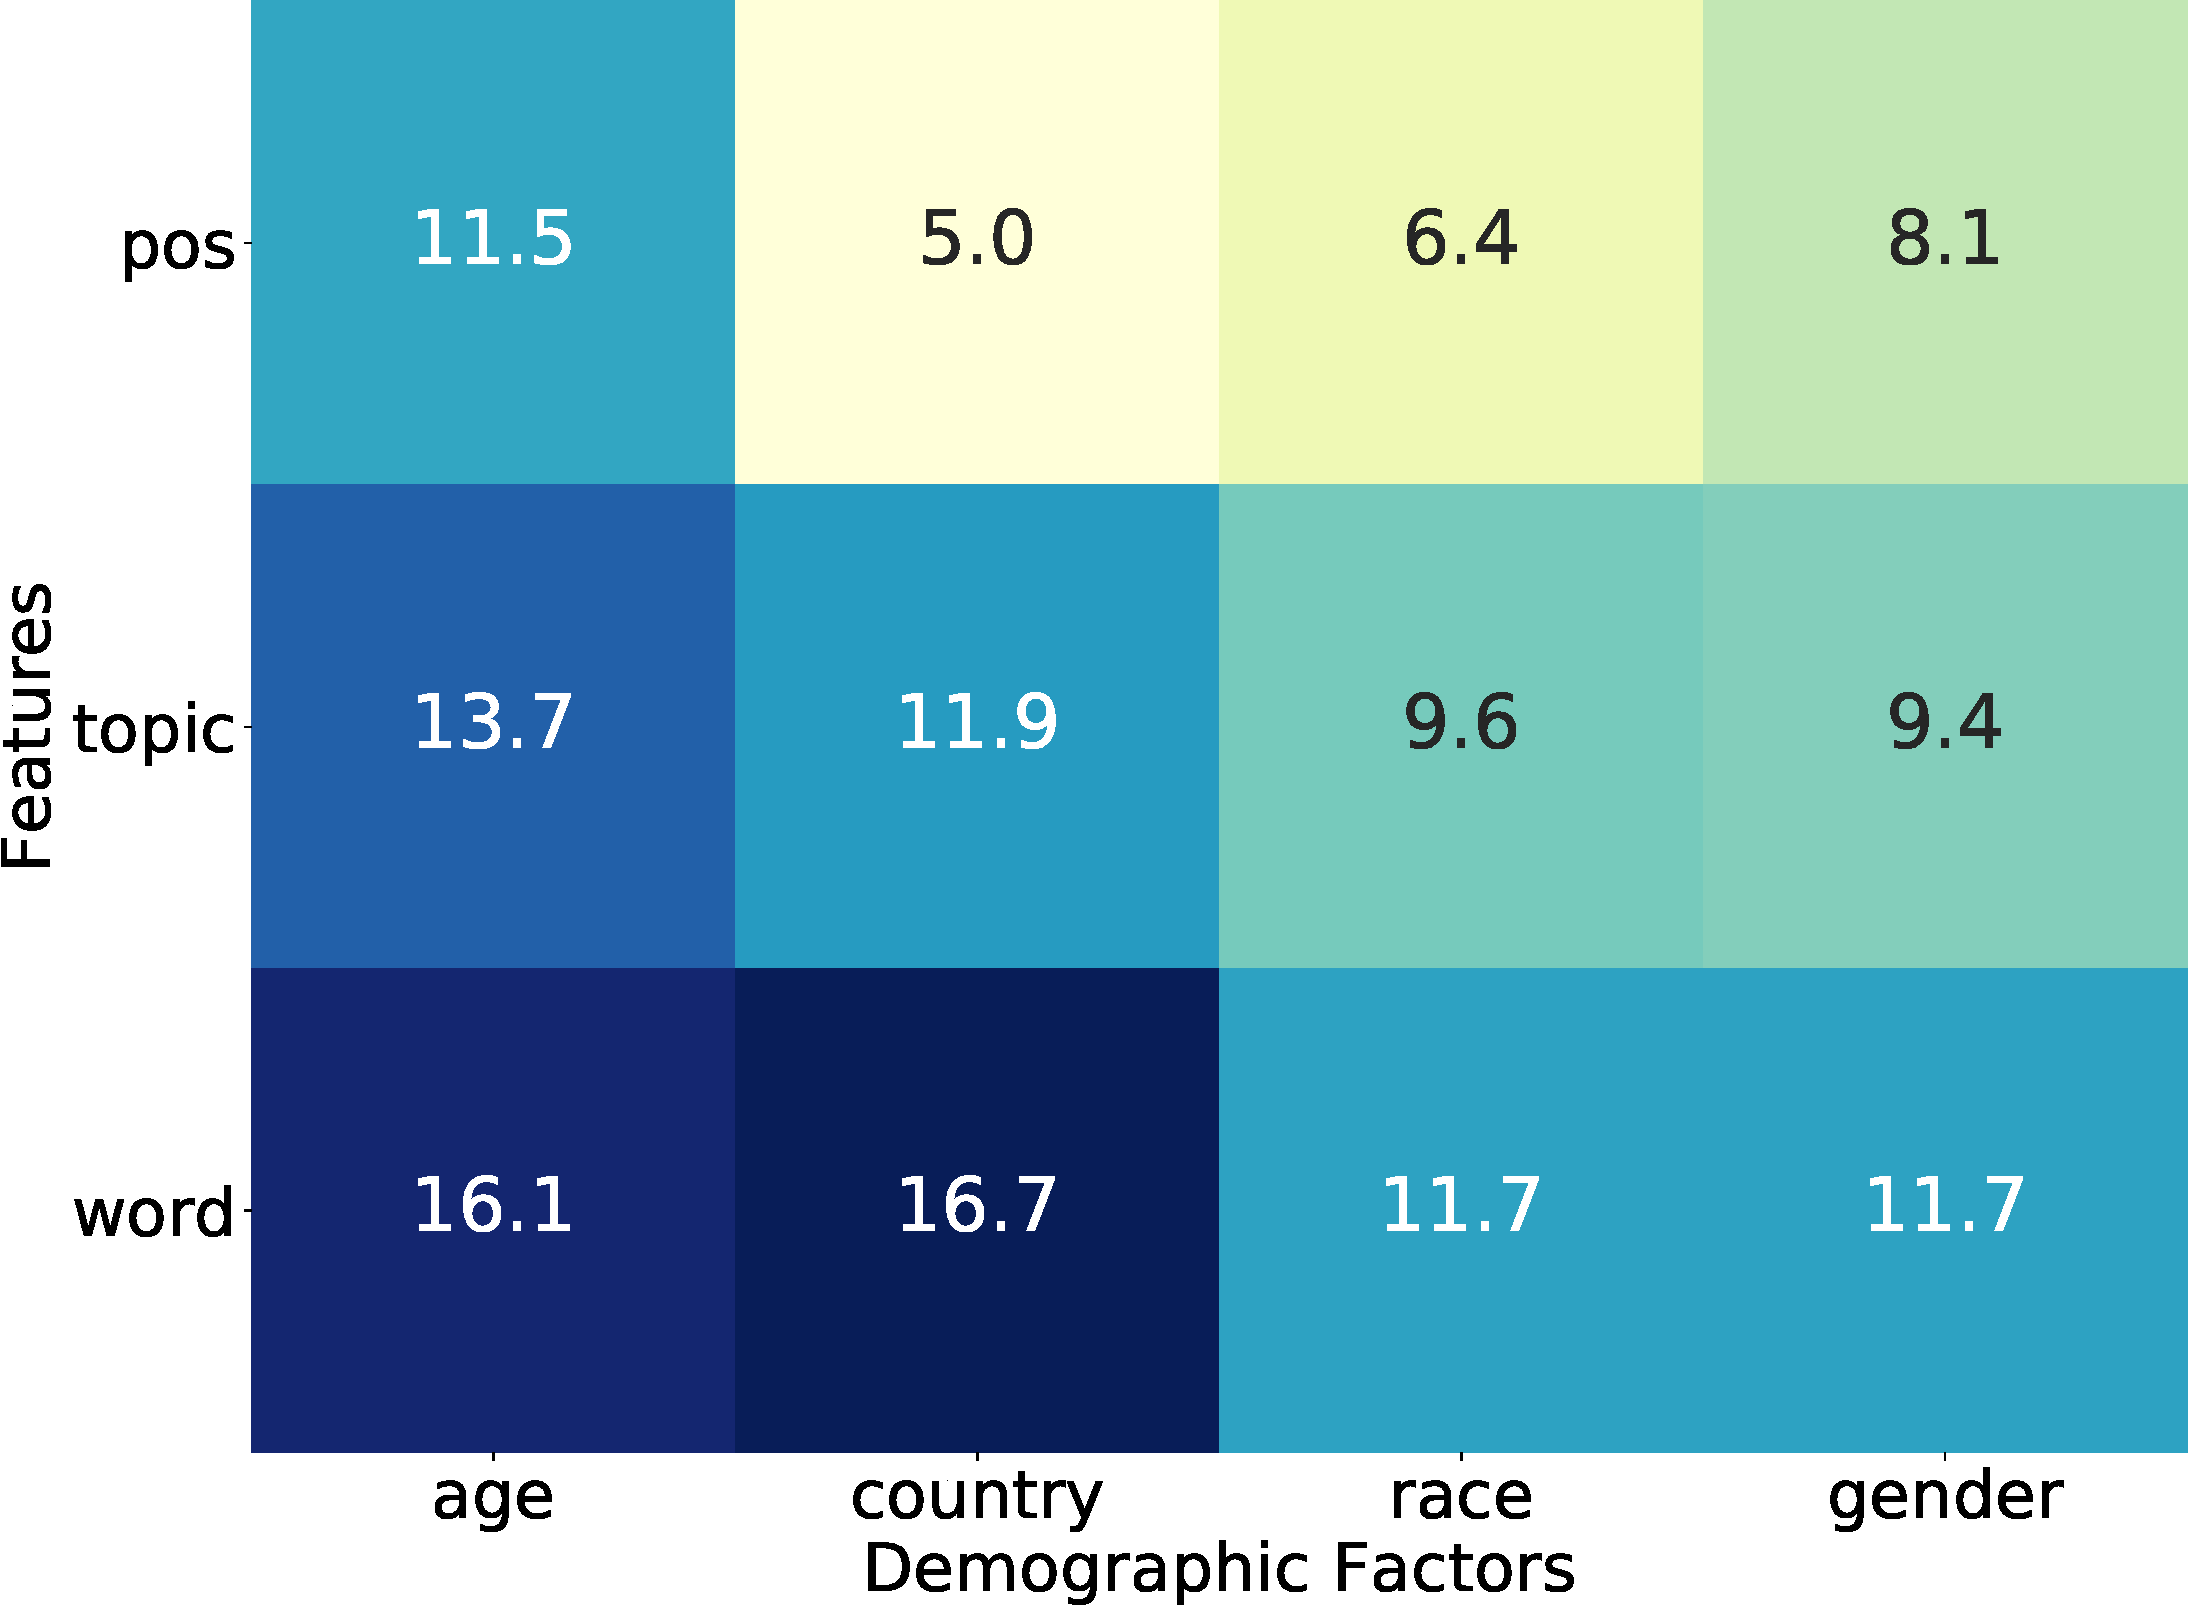
\includegraphics[width=0.55\textwidth]{images/chapter5/predictability.pdf}
\caption{Predictability of demographic attributes from language
data. We show the absolute percentage improvements in accuracy over majority-class baselines. The majority-class baselines of accuracy scores are either .500 for the binary prediction or .250 for the US region prediction. The darker color indicates higher improvements and vice versa.}
\label{fig:predictability}
\end{figure}

The improved prediction accuracy scores over majority baselines suggest that language variations across demographic groups are encoded in the text documents. 
The results show that documents are the most predictable to the age attribute.
We can also observe that the word is the most predictable feature to demographic factors,
while the POS feature is least predictable towards the country factor.
These suggest there might be a connection between language variations and demographic groups.
This motivates us to further explore the language variations based on word features.
We rank the word features by mutual information classification~\cite{pedregosa2011scikit} and present the top 10 unigram features in Table~\ref{tab:features}.
The qualitative results show the most predictable word features towards the demographic groups and 
suggest such variations may impact extracted feature representations and further training document classifiers.

% discuss the findings
The Table~\ref{tab:features} shows that when classifying hate speech tweets, the n-words and b-words are more significant correlated with the white instead of the other racial groups.
However, this shows an opposite view than the existing work~\cite{davidson2019racial}, which presents the two types of words are more significantly correlated with the black.
This can highlight the values of our approach that to avoid confounding errors, we obtain author demographic information independently from the user generated documents.



\subsection{Do Demographic Groups Express Document Categories Differently?}
Textual features, which are fundamental to build document classifiers, inherently vary across different demographic attributes, such as gender, age, location and political orientation~\cite{gao2015more,hinds2018demographic}.
Expressing differently between demographic groups to show the same sentiments will confuse document classifiers and lead to biased classifiers.
For example, balancing sensitive word features increase the biases of document classifiers~\cite{dixon2018measuring}.
Therefore, this motivates us to explore if textual features that are extracted for document classifiers vary across demographic groups.

To compare and measure demographic variations of textual features, we conduct comparisons on three different levels:

\paragraph{Word-level.} For each demographic group, we extract n-gram features (same feature sets as in the previous subsection) that are most associated with the document labels. With mutual information, we select the top 1,000 features for each group. Within each demographic attribute, we then calculate the percentage of overlap across different groups (e.g., males and females in gender factor): if $F_0$ is the set of top features for one factor and $F_1$ is the set of top features for another factor, the percent overlap is calculated as $|F_0 \cap F_1|/1000$.

\paragraph{POS-level.} For each demographic group, we extract and aggregate POS features (same feature sets as in the previous subsection). After normalizing the accumulated features, we can obtain POS representations for each demographic group. Within each demographic factor, we use Wasserstein distance to measure the distributional distance. Wasserstein distance or Earth Mover's distance~\cite{vallender1974calculation} is to measure the distributional differences between source and target domains in domain adaptation. In this study, we treat each demographic factor as a domain, and use the Wasserstein distance to measure demographic variations.

\paragraph{Topic-level.} For each demographic group, we use the trained topic model (same as in the previous subsection) to extract and calculate the average topic distribution across documents from that group. Then within each demographic factor, we measure language variations across demographic groups by Wasserstein distance. Particularly, to keep consistently binary values across demographic factors, we binarize the four regional values (MW + W and NE + S).

\begin{figure}[htp]
\centering
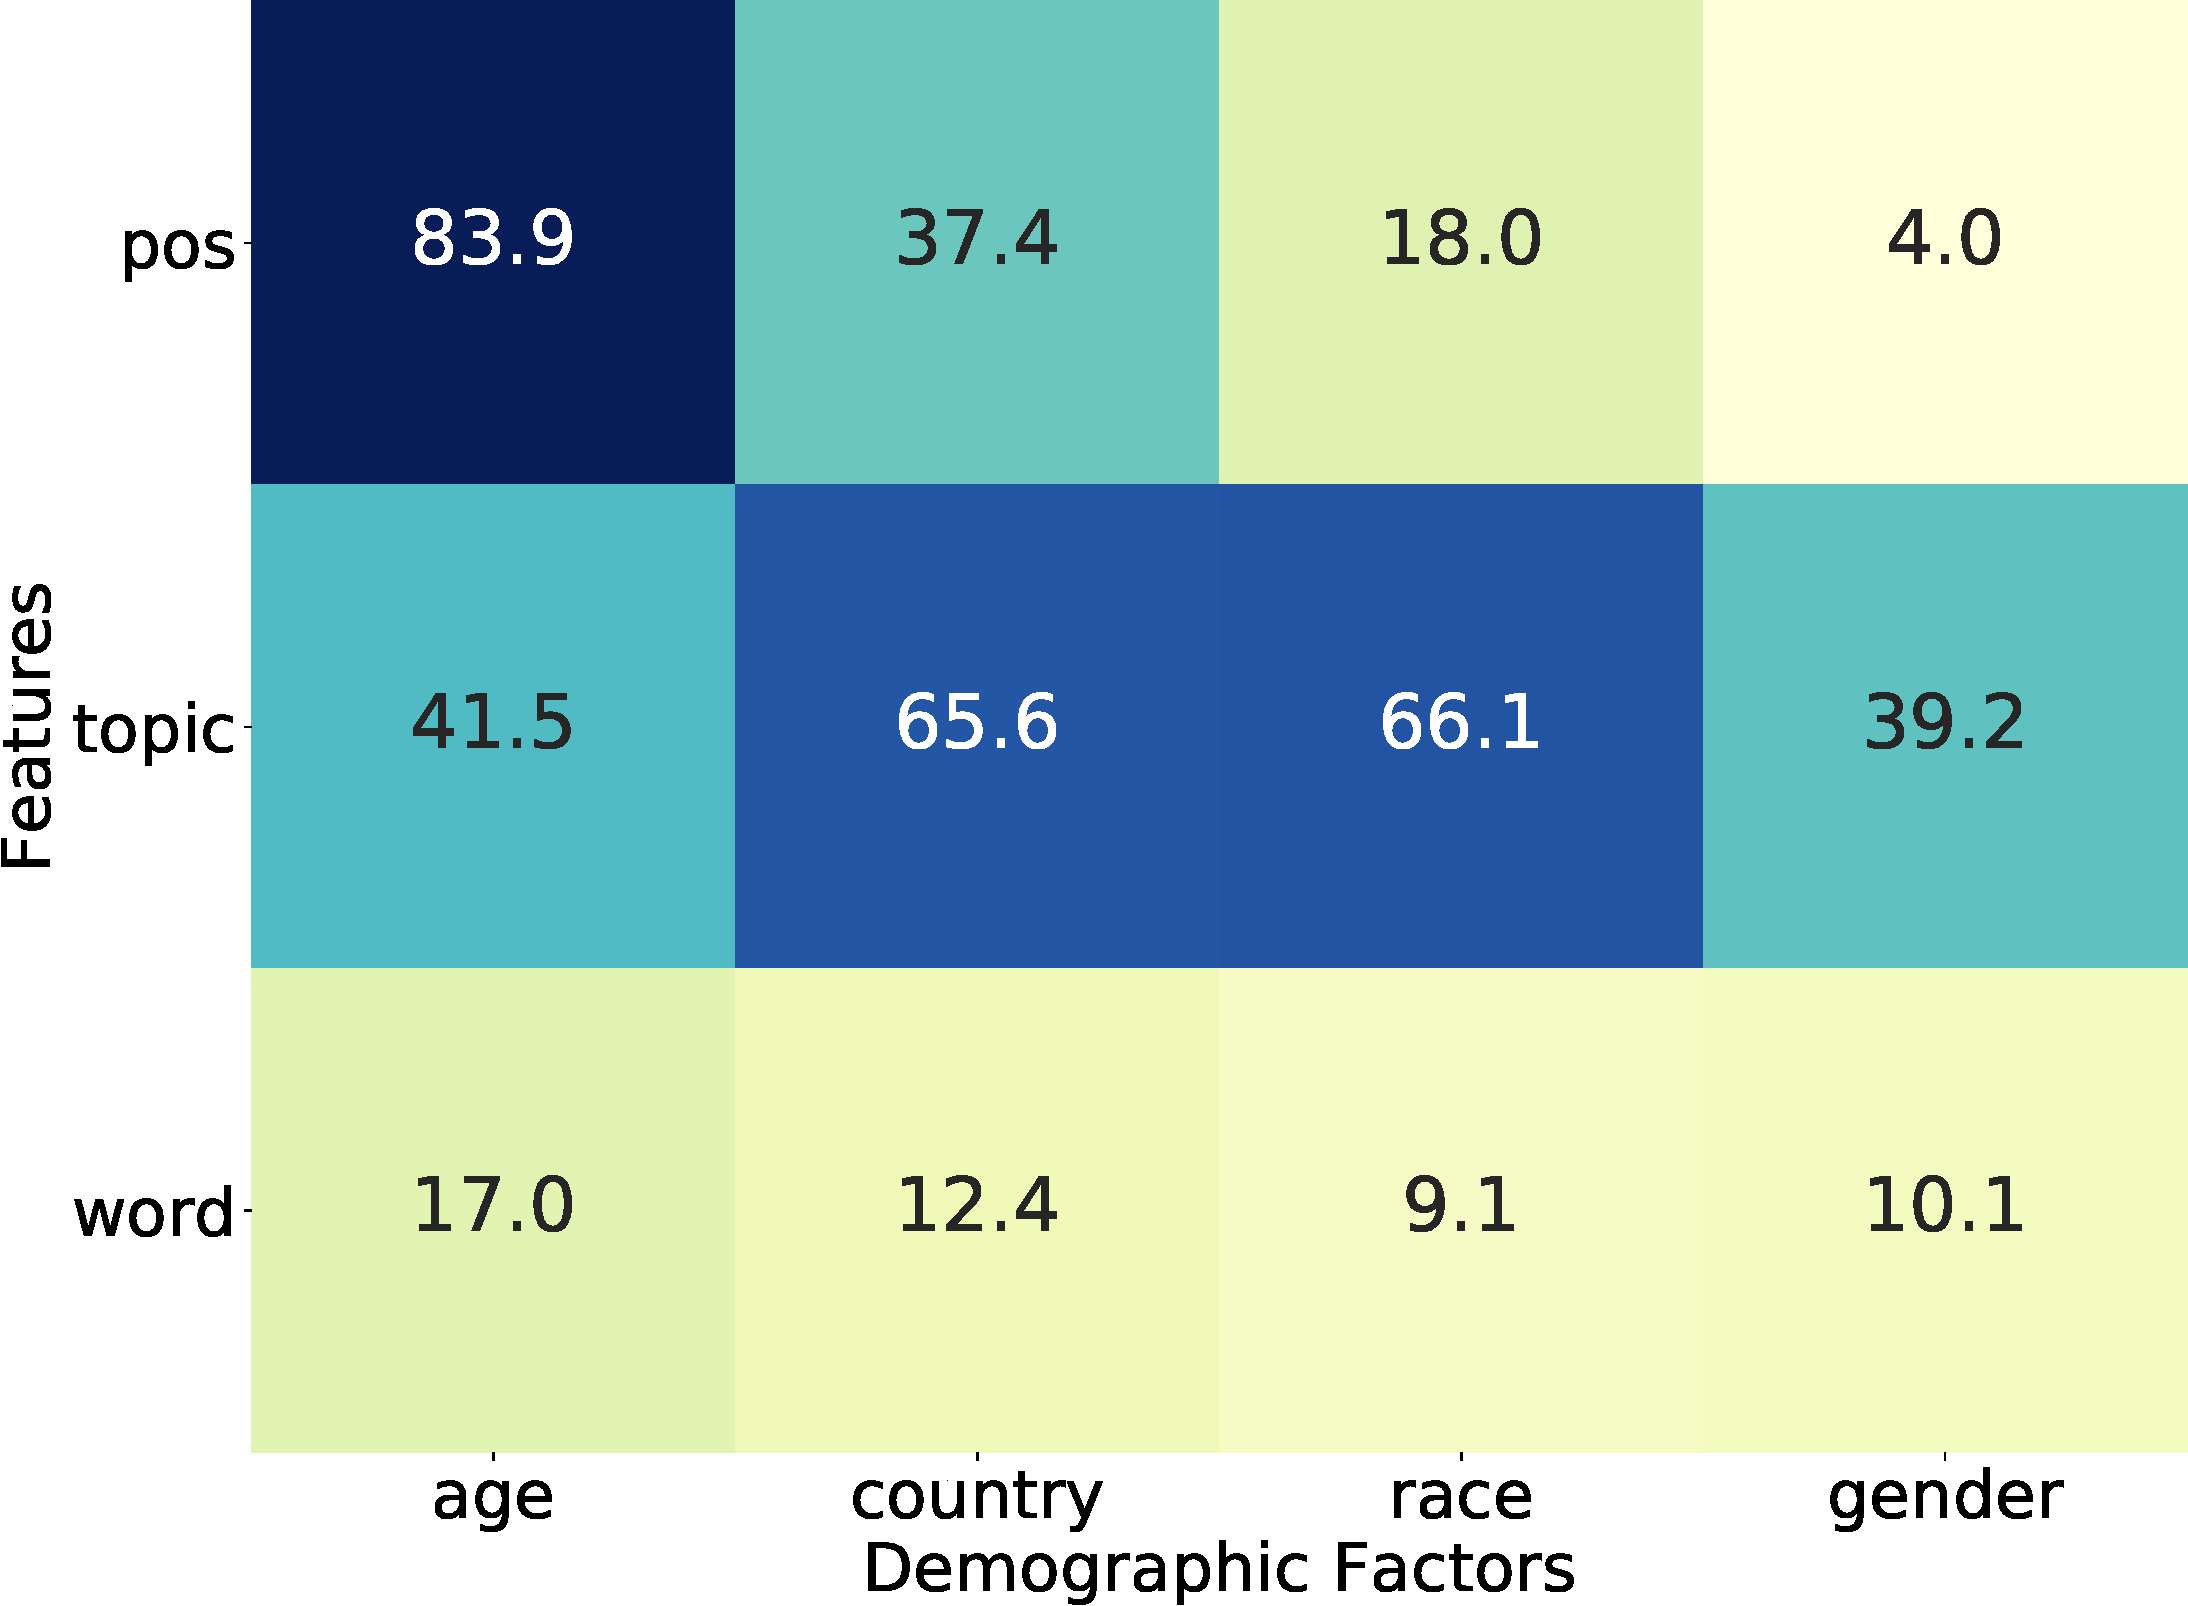
\includegraphics[width=0.55\textwidth]{images/chapter5/overlaps.pdf}
\caption{Language variations on how people express sentiment differently are calculated for each demographic factor. Darker color indicates more variations in expressing sentiments being classified.}
\label{fig:overlaps}
\end{figure}

To measure fairly expression variations, we randomly sample two groups of documents for each demographic factor as comparison sets. 
We calculate the overlaps and distances on the randomly sampled sets. 
We then compare percentage differences of the overlaps and distance scores between the demographic factors and the randomly selected sets: if $S_d$ is the overlap or distance score of one factor and $S_r$ is the score from the random comparison group, the percentage difference is calculated as $|S_d - S_r|/S_r$.
Results are visualized in Figure~\ref{fig:overlaps}. 
Higher percentage differences indicate higher variations across demographic groups express sentiments.
We can observe there are more variations in age and region from the topic and POS levels.


\section{Experiments}

Demographic variations root in documents, especially in social media data~\cite{volkova2013exploring,hovy2015demographic,johannsen2015cross}.
Such variations could further impact the performance and fairness of document classifiers.
In this study, we experiment four different classification models including logistic regression (LR), recurrent neural network (RNN)~\cite{chung2014empirical}, convolutional neural network (CNN)~\cite{kim2014convolutional} and Google BERT~\cite{devlin2019bert}.
We present the baseline results of both performance and fairness evaluations across the multilingual corpus.

\subsection{Data Preprocessing}
To anonymize user information, we hash user and tweet ids and then replace hyperlinks, usernames, and hashtags with generic symbols (URL, USER, HASHTAG).
Documents are lowercased and tokenized using NLTK~\cite{bird2004nltk}. 
The corpus is randomly split into training (70\%), development (15\%), and test (15\%) sets. 
We train the models on the training set and find the optimal hyperparameters on the development set before final evaluations on the test set. 
We randomly shuffle the training data at the beginning of each training epoch.

\begin{table*}[htp]
\centering
\resizebox{.48\columnwidth}{!}{
\begin{tabular}{cc|cccc}
Language & Method & Acc & F1-w & F1-m & AUC \\\hline
\multirow{4}{*}{English} & LR & .874 & .874 & .841 & .920 \\
 & CNN & .878 & .877 & .845 & .927 \\
 & RNN & \textbf{.898} & \textbf{.896} & \textbf{.867} & \textbf{.938} \\
 & BERT & .705 & .635 & .579 & .581
\end{tabular}
}
\quad
\resizebox{.48\columnwidth}{!}{
\begin{tabular}{cc|cccc}
Language & Method & Acc & F1-w & F1-m & AUC \\\hline
\multirow{4}{*}{Italian} & LR & .660 & .679 & .631 & .725 \\
 & CNN & .687 & .702 & .651 & .745 \\
 & RNN & \textbf{.729} & \textbf{.731} & \textbf{.666} & \textbf{.763} \\
 & BERT & .697 & .629 & .468 & .498
\end{tabular}
}

\resizebox{.48\columnwidth}{!}{
\begin{tabular}{cc|cccc}
\multicolumn{6}{c}{} \\
Language & Method & Acc & F1-w & F1-m & AUC \\\hline
\multirow{4}{*}{Polish} & LR & \textbf{.864} & .846 & .653 & .804 \\
 & CNN & .855 & .851 & .688 & .813 \\
 & RNN & .857 & \textbf{.854} & \textbf{.696} & \textbf{.822} \\
 & BERT & .824 & .782 & .478 & .474
\end{tabular}
}
\quad
\resizebox{.48\columnwidth}{!}{
\begin{tabular}{cc|cccc}
\multicolumn{6}{c}{} \\
Language & Method & Acc & F1-w & F1-m & AUC \\\hline
\multirow{4}{*}{Portuguese} & LR & .660 & .598 & .551 & .648 \\
 & CNN & \textbf{.681} & \textbf{.674} & \textbf{.653} & \textbf{.719} \\
 & RNN & .607 & .586 & .553 & .633 \\
 & BERT & .613 & .568 & .525 & .524
\end{tabular}
}

\begin{tabular}{cc|cccc}
\multicolumn{6}{c}{} \\
Language & Method & Acc & F1-w & F1-m & AUC \\\hline
\multirow{4}{*}{Spanish} & LR & \textbf{.704} & \textbf{.707} & \textbf{.698} & \textbf{.761} \\
 & CNN & .650 & .654 & .645 & .710\\
 & RNN & .674 & .674 & .658 & .720 \\
 & BERT & .605 & .573 & .502 & .505
\end{tabular}
\caption{Overall performance evaluation of baseline classifiers. We evaluate overall performance by four metrics including accuracy (Acc), weighted F1 score (F1-w), macro F1 score (F1-m) and area under the ROC curve (AUC). The higher score indicates better performance. We highlight models achieve the best performance in each column.}
\label{tab:perform}
\end{table*}


\subsection{Baseline Models}
We implement and experiment four baseline classification models. 
To compare fairly, we keep the feature size up to 15K for each classifier across all five languages.
We calculate the weight for each document category by $\frac{N}{N_l}$~\cite{king2001logistic}, where $N$ is the number of documents in each language and $N_l$ is the number of documents labeled by the category.
Particularly, for training BERT model, we append two additional tokens, ``[CLS]'' and ``[SEP]'', at the start and end of each document respectively.
For the neural models, we pad each document or drop rest of words up to 40 tokens.
We use ``unknown'' as a replacement for unknown tokens.
We initialize CNN and RNN classifiers by pre-trained word embeddings~\cite{mikolov2013distributed,godin2015multimedia,bojanowski2017enriching,deriu2017leveraging} and train the networks up to 10 epochs.

\paragraph{LR.} 
We first extract TF-IDF-weighted features of uni-, bi-, and tri-grams on the corpora, using the most frequent 15K features with the minimum feature frequency as 2. 
We then train a \texttt{LogisticRegression} from scikit-learn~\cite{pedregosa2011scikit}. 
We use ``liblinear'' as the solver function and leave the other parameters as default.

\paragraph{CNN.} 
We implement the Convolutional Neural Network (CNN) classifier described in~\cite{kim2014convolutional,zimmerman2018improving} by Keras~\cite{chollet2015keras}.
We first apply 100 filters with three different kernel sizes, 3, 4 and 5.
After the convolution operations, we feed the concatenated features to a fully connected layer and output document representations with 100 dimensions.
We apply ``softplus'' function with a l2 regularization with $.03$ and a dropout rate with $.3$ in the dense layer.
The model feeds the document representation to final prediction.
We train the model with batch size 64, set model optimizer as Adam~\cite{kingma2014adam} and calculate loss values by the cross entropy function.
We keep all other parameter settings as described in the paper~\cite{kim2014convolutional}.


\paragraph{RNN.}
We build a recurrent neural network (RNN) classifier by using bi-directional Gated Recurrent Unit (bi-GRU)~\cite{chung2014empirical,park2018reducing}.
We set the output dimension of GRU as 200 and apply a dropout on the output with rate $.2$.
We optimize the RNN with RMSprop~\cite{tieleman2012lecture} and use the same loss function and batch size as the CNN model.
We leave the other parameters as default in the Keras~\cite{chollet2015keras}.


\paragraph{BERT}
BERT is a transformer-based pre-trained language model which was well trained on multi-billion sentences publicly available on the web~\cite{devlin2019bert}, which can effectively generate the precise text semantics and useful signals.
We implement a BERT-based classification model by HuggingFace's Transformers~\cite{Wolf2019HuggingFacesTS}.
The model encodes each document into a fixed size (768) of representation and feed to a linear prediction layer.
The model is optimized by \texttt{AdamW} with a warmup and learning rate as $.1$ and $2e^{-5}$ respectively.
We leave parameters as their default, conduct fine-tuning steps with 4 epochs and set batch size as 32~\cite{sun2019fine}.
The classification model loads ``bert-base-uncased'' pre-trained BERT model for English and ``bert-base-multilingual-uncased'' multilingual BERT model~\cite{gertner2019mitre} for the other languages.
The multilingual BERT model follows the same method of BERT by using Wikipedia text from the top 104 languages.
Due to the label imbalance shown in Table~\ref{tab:corpus}, we balance training instances by randomly oversampling the minority during the training process.


\subsection{Evaluation Metrics}

\paragraph{Performance Evaluation.}
To measure overall performance, we evaluate models by four metrics: accuracy (Acc), weighted F1 score (F1-w), macro F1 score (F1-m) and area under the ROC curve (AUC). %\footnote{We used implementations from scikit-learn~\cite{pedregosa2011scikit}.}
The F1 score coherently combines both precision and recall by $2*\frac{precision*recall}{precision+recall}$.
We report F1-m considering that the datasets are imbalanced.

\paragraph{Fairness Evaluation.}
To evaluate {group fairness}, we measure the \textit{equality differences} (ED) of true positive/negative and false positive/negative rates for each demographic factor. 
ED is a standard metric to evaluate fairness and bias of document classifiers~\cite{dixon2018measuring,park2018reducing,garg2019counterfactual}.

This metric sums the differences between the rates within specific user groups and the overall rates.
Taking the false positive rate (FPR) as an example, we calculate the equality difference by:
$$FPED = \sum_{d \in D}|FPR_d - FPR|$$
, where $D$ is a demographic factor (e.g., race) and $d$ is a demographic group (e.g., white or nonwhite).


\section{Results}
We have presented our evaluation results of performance and fairness in Table~\ref{tab:perform} and Table~\ref{tab:fairness} respectively.
Country and race have very skewed distributions in the Italian and Polish corpora, therefore, we omit fairness evaluation on the two factors.

\begin{table*}[htp]
\centering
\footnotesize
\begin{tabular}{cc|ccc}
\multicolumn{5}{c}{\textbf{Age}} \\\hline\hline
Language & Method & FNED & FPED & SUM-ED\\\hline
\multirow{4}{*}{English} & LR & .059 & .104 & .163\\
 & CNN  & .052 & .083 & .135 \\
 & RNN  & .041 & .118 & .159 \\
 & BERT & .004 & .012 & .016 
\end{tabular}
\quad
\begin{tabular}{cc|ccc}
\multicolumn{5}{c}{\textbf{Gender}} \\\hline\hline
Language & Method & FNED & FPED & SUM-ED \\\hline
\multirow{4}{*}{English} & LR & .023 & .056 & .079 \\
 & CNN  & .018 & .056 & .074 \\
 & RNN  & .013 & .055 & .068 \\
 & BERT & .007 & .009 & .016
\end{tabular}

\begin{tabular}{cc|ccc}
\multicolumn{5}{c}{} \\\hline\hline
Language & Method & FNED & FPED & SUM-ED \\\hline
\multirow{4}{*}{Italian} & LR & .076 & .194 & .270\\
 & CNN  & .003 & .211 & .214\\
 & RNN  & .042 & .185 & .227\\
 & BERT & .029 & .034 & .063
\end{tabular}
\quad
\begin{tabular}{cc|ccc}
\multicolumn{5}{c}{} \\\hline\hline
Language & Method & FNED & FPED & SUM-ED \\\hline
\multirow{4}{*}{Italian} & LR  & .145 & .020 & .165 \\
 & CNN  & .064 & .094 & .158 \\
 & RNN  & .088 & .075 & .163 \\
 & BERT & .041 & .056 & .097
\end{tabular}

\begin{tabular}{cc|ccc}
\multicolumn{5}{c}{} \\\hline\hline
Language & Method & FNED & FPED & SUM-ED \\\hline
\multirow{4}{*}{Polish} & LR & .256 & .059 & .315 \\
 & CNN  & .389 & .138 & .527 \\
 & RNN  & .335 & .089 & .424 \\
 & BERT & .027 & .027 & .054
\end{tabular}
\quad
\begin{tabular}{cc|ccc}
\multicolumn{5}{c}{} \\\hline\hline
Language & Method & FNED & FPED & SUM-ED \\\hline
\multirow{4}{*}{Polish} & LR & .266 & .045 & .309 \\
 & CNN  & .411 & .048 & .459 \\
 & RNN  & .340 & .034 & .374 \\
 & BERT & .042 & .013 & .055
\end{tabular}

\begin{tabular}{cc|ccc}
\multicolumn{5}{c}{} \\\hline\hline
Language & Method & FNED & FPED & SUM-ED \\\hline
\multirow{4}{*}{Portuguese} & LR  & .061 & .044 & .105 \\
 & CNN  & .033 & .096 & .129 \\
 & RNN  & .079 & .045 & .124 \\
 & BERT & .090 & .097 & .187 
\end{tabular}
\quad
\begin{tabular}{cc|ccc}
\multicolumn{5}{c}{} \\\hline\hline
Language & Method & FNED & FPED & SUM-ED \\\hline
\multirow{4}{*}{Portuguese} & LR  & .052 & .007 & .059 \\
 & CNN  & .018 & .013 & .031 \\
 & RNN  & .099 & .083 & .182 \\
 & BERT & .055 & .125 & .180
\end{tabular}

\begin{tabular}{cc|ccc}
\multicolumn{5}{c}{} \\\hline\hline
Language & Method & FNED & FPED & SUM-ED \\\hline
\multirow{4}{*}{Spanish} & LR & .089 & .013 & .102 \\
 & CNN  & .117 & .139 & .256 \\
 & RNN  & .078 & .083 & .161 \\
 & BERT & .052 & .015 & .067
\end{tabular}
\quad
\begin{tabular}{cc|ccc}
\multicolumn{5}{c}{} \\\hline\hline
Language & Method & FNED & FPED & SUM-ED \\\hline
\multirow{4}{*}{Spanish} & LR & .131 & .061 & .292 \\
 & CNN  & .032 & .108 & .140 \\
 & RNN  & .030 & .039 & .069 \\
 & BERT & .021 & .016 & .037
\end{tabular}

\begin{tabular}{cc|ccc}
\multicolumn{5}{c}{} \\
\multicolumn{5}{c}{} \\
\multicolumn{5}{c}{\textbf{Country}} \\\hline\hline
Language & Method & FNED & FPED & SUM-ED \\\hline
\multirow{4}{*}{English} & LR & .026 & .053 & .079 \\
 & CNN  & .027 & .063 & .090\\
 & RNN  & .024 & .061 & .085\\
 & BERT & .006 & .001 & .007
\end{tabular}
\quad
\begin{tabular}{cc|ccc}
\multicolumn{5}{c}{} \\
\multicolumn{5}{c}{} \\
\multicolumn{5}{c}{\textbf{Race}} \\\hline\hline
Language & Method & FNED & FPED & SUM-ED \\\hline
\multirow{4}{*}{English} & LR  & .019 & .056 & .075 \\
 & CNN  & .007 & .029 & .036 \\
 & RNN  & .008 & .063 & .071 \\
 & BERT & .003 & .009 & .012 
\end{tabular}

\begin{tabular}{cc|ccc}
\multicolumn{5}{c}{} \\\hline\hline
Language & Method & FNED & FPED \\\hline
\multirow{4}{*}{Portuguese} & LR & .093 & .026 & .119\\
 & CNN  & .110 & .122 & .232 \\
 & RNN  & .022 & .004 & .026 \\
 & BERT & .073 & .071 & .144
\end{tabular}
\quad
\begin{tabular}{cc|ccc}
\multicolumn{5}{c}{} \\\hline\hline
Language & Method & FNED & FPED & SUM-ED \\\hline
\multirow{4}{*}{Portuguese} & LR  & .068 & .005 & .073 \\
 & CNN  & .056 & .033 & .089 \\
 & RNN  & .074 & .054 & .128 \\
 & BERT & .045 & .186 & .231
\end{tabular}

\begin{tabular}{cc|ccc}
\multicolumn{5}{c}{} \\\hline\hline
Language & Method & FNED & FPED & SUM-ED \\\hline
\multirow{4}{*}{Spanish} & LR & .152 & .154 & .306\\
 & CNN  & .089 & .089 & .178 \\
 & RNN  & .071 & .113 & .184 \\
 & BERT & .017 & .017 & .034
\end{tabular}
\quad
\begin{tabular}{cc|ccc}
\multicolumn{5}{c}{} \\\hline\hline
Language & Method & FNED & FPED & SUM-ED \\\hline
\multirow{4}{*}{Spanish} & LR & .095 & .030 & .125 \\
 & CNN  & .072 & .054 & .126 \\
 & RNN  & .011 & .004 & .015 \\
 & BERT & .046 & .005 & .051
\end{tabular}
\caption{Fairness evaluation of baseline classifiers across the five languages on the four demographic factors. We measure fairness and bias of document classifiers by equality differences of false negative rate (FNED), false positive rate (FPED) and sum of FNED and FPED (SUM-ED). The higher score indicates lower fairness and higher bias and vice versa.}
\label{tab:fairness}
\end{table*}

\paragraph{Overall performance evaluation.}
Table~\ref{tab:perform} demonstrates the performances of the baseline classifiers for hate speech classification on the corpus we proposed. 
Results are obtained from the five languages covered in our corpus respectively.
Among the four baseline classifiers, LR, CNN and RNN consistently perform well on all languages.
Moreover, neural-based models (CNN and RNN) substantially outperform LR on four out of five languages (except Spanish).
However, the results obtained by BERT are relatively lower than the other baselines, and show more significant gap in the English dataset.
One possible explanation is BERT was pre-trained on Wikipedia documents, which are significantly different from the Twitter corpus in document length, word usage and grammars.
For example, each tweet is a short document with 20 tokens, but the BERT is trained on long documents up to 512 tokens.
Existing research suggests that fine-tuning on the multilingual corpus can further improve performance of BERT models~\cite{sun2019fine}.


% low performance of bert on the polish data~\cite{korzeniowski2019exploiting}

\paragraph{Group fairness evaluation.}

% reference:
We have measured the group fairness in Table~\ref{tab:fairness}. 
% RNN achieves lower sum-ed scores across major evaluation tasks.
Generally, the RNN classifier achieves better and more stable performance across major fairness evaluation tasks.
By comparing the different baseline classifiers, we can find out that the LR usually show stronger biases than the neural classification models among majority of the tasks.
While the BERT classifier performs comparatively lower accuracy and F1 scores, the classifier has less biases on the most of the datasets.
However, biases can significantly increases for the Portuguese dataset when the BERT classifier achieves better performance.
%A trade-off relationship usually exists between accuracy and model performance~\cite{menon2018cost}.
We examine the relationship by building linear model between two differences: the performance differences between the RNN and other classifiers, the SUM-ED differences between RNN and other classifiers.
We find that the classification performance does not have significantly ($p-value > .05$) correlation with fairness and bias.
The significant biases of classifiers varies across tasks and languages: the classifiers trained on Polish and Italian are biased the most by Age and Gender, the classifiers trained on Spanish and Portuguese are most biased the most by Country, and the classifiers trained on English tweets are the most unbiased throughout all the attributes.
Classifiers usually have very high bias scores on both gender and age in Italian and Polish data.
We find that the age and gender both have very skewed distributions in the Italian and Polish datasets. 
Overall, our baselines provide a promising start for evaluating future new methods of reducing demographic biases for document classification under the multilingual setting.


\section{Domain Adaptation Experiments}
Demographic variations root in documents, especially in social media data~\cite{volkova2013exploring,hovy2015demographic}.
Our previous analyses demonstrate language varies substantially across demographic groups.
Such variations could further impact the fairness of document classifiers.
In this study, we present a standard domain adaptation model that within each demographic factor, we treat each demographic group as a domain (e.g., male and female domains).
We show the domain adaptation method can effectively reducing the biases of document classifiers on five demographic attributes: age, gender, race, country and US region.

\subsection{Data Preprocessing}
We replace hyperlinks, usernames, and hashtags with generic symbols. Documents are lowercased and tokenized using NLTK~\cite{bird2004nltk}. 
The corpus is randomly split into training (80\%), development (10\%), and test (10\%) sets. 
We train the models on the training set and find the optimal hyperparameters on the development set. 
We randomly shuffle the training data at the beginning of each training epoch. 
%The evaluation metric is weighted F1 score.

\subsection{Classification Models}
We experiment with two classifiers, with more details in the supplement.
We use logistic regression (\textbf{LR}) as a non-neural classifier,
implemented with scikit-learn~\cite{pedregosa2011scikit} with its default parameters.
We use a Gated Recurrent Unit (\textbf{GRU})~\cite{chung2014empirical} as a neural model, which achieves the best performance in previous fairness evaluation of document classification on the token level~\cite{park2018reducing}. 
To be consistent with this prior work, we implement the same model and initialize it with same word embeddings, implemented in Keras~\cite{chollet2015keras}.

\subsection{Model Settings}

\paragraph{LR, FEDA.} We first extract domain-specific and general representations as TF-IDF-weighted n-gram (1-, 2-grams) features with minimum feature frequency as 2. For the FEDA, we extract the top 8K features for each domain and the general feature sets.
For the ``fair'' mode, we formalize a document representation by averaging the representations of all words in that document.
We train logistic regression classifiers using the \texttt{LogisticRegression} implementation in Scikit-learn~\cite{pedregosa2011scikit} with default parameters.
To select the best models, we tune parameters by the F1-weighted score on the validation set.

\paragraph{GRU.} We use Keras~\cite{chollet2015keras} to implement the bidirectional recurrent neural model. 
We optimize the model by \textit{RMSprop}~\cite{tieleman2012lecture} and calculate the loss by \textit{binary\_crossentropy} from the Keras.
We set the class weight as ``auto'' and leave the other parameters as defaults.
To keep consistent, we keep the 8K most frequent words and replace the other words as an ``unk'' token.
We pad each document to a length of 30.
We train the model with 20 epochs and a batch size of 64. 
After each training epoch, we evaluate and choose the best model on the validation set by the F1-weighted score.


\subsection{Evaluation Metrics}

We use weighted F1 score and area under the ROC curve (AUC) to measure overall performance.
To evaluate {group fairness},
we measure the \textit{equality differences} (ED) of true positive/negative and false positive/negative rates~\cite{dixon2018measuring,park2018reducing,garg2019counterfactual} for each demographic factor. 
This metric sums the differences between the rates within specific user groups and the overall rates.
Taking the false positive rate (FPR) as an example, we calculate the equality difference by $FPED = \sum_{d \in D}|FPR_d - FPR|$, where $D$ is a demographic factor (e.g., race) and $d$ is a demographic group (e.g., white or nonwhite).


\begin{table*}[t!]
\centering
%\resizebox{1\columnwidth}{!}{
\begin{tabular}{l||cc|cc}
\multicolumn{5}{c}{\bf Gender} \\\hline
&F1&AUC&FNED&FPED\\\hline\hline
%\multicolumn{5}{c}{Traditional Model} \\\hline
LR& .831 & \bf .881 & .027 & .007 \\
+blind& .831 & .880 & .028 & .004\\
+fair& .797 & .859 & .026 & .005 \\
+swap& .830 & \bf .881 & .029 & .007 \\
+FEDA& \bf .840 & .879 & \bf .016 & \bf .002\\
\hline
%\multicolumn{5}{c}{Neural Model} \\\hline
GRU& .764 & .841 & .037 & .056 \\
+blind& .769 & .837 & .054 & .036\\
+fair& .794 & .843 & .051 & .003\\
+swap& .797 & .844 & .040 & .026\\\hline
%\multicolumn{7}{c}{With adaptation} \\\hline
\end{tabular}
%}
\quad
%\resizebox{1\columnwidth}{!}{
\begin{tabular}{l||cc|cc}
\multicolumn{5}{c}{\bf Age} \\\hline
&F1&AUC&FNED&FPED\\\hline\hline
%\multicolumn{5}{c}{Traditional Model} \\\hline
LR& .838 & .885 & .260 & .014\\
+blind& .835 & \bf .886 & .266 & .013 \\
+fair& .807 & .859 & .229 & .040\\
+swap& .836 & .884 & .266 & .008\\
+FEDA& \bf .842 & .883 & .280 & \bf .004\\
\hline
%\multicolumn{5}{c}{Neural Model} \\\hline
GRU& .744 & .839 & \bf .132 & .042\\
+blind& .781 & .831 & .188 & .045 \\
+fair& .770 & .821 & .178 & .019 \\
+swap& .779 & .837 & .203 & .022 \\\hline
%\multicolumn{5}{c}{With adaptation} \\\hline
\end{tabular}
%}

%\resizebox{1\columnwidth}{!}{
\begin{tabular}{l||cc|cc}
\multicolumn{5}{c}{\bf Country} \\\hline
&F1&AUC&FNED&FPED\\\hline\hline
%\multicolumn{5}{c}{Traditional Model} \\\hline
LR& .801 & .847 & .086 & .002\\
+blind& .800 & .846 & .086 & .003\\
+fair& .773 & .825 & .090 & \bf .001\\
+swap& .801 & .846 & .090 & .003\\
+FEDA& \bf .812 & \bf .848 & .080 & .008\\
\hline
%\multicolumn{5}{c}{Neural Model} \\\hline
GRU & .758 & .793 & .079 & \bf .001 \\
+blind& .759 & .791 & .109 & .003\\
+fair& .746 & .794 & \bf .076 & .011\\
+swap& .746 & .780 & .080 & .008 \\\hline
%\multicolumn{5}{c}{With adaptation} \\\hline
\end{tabular}
%}
\quad
%\resizebox{1\columnwidth}{!}{
\begin{tabular}{l||cc|cc}
\multicolumn{5}{c}{\bf US Region} \\\hline
&F1&AUC&FNED&FPED\\\hline\hline
% \multicolumn{5}{c}{Traditional Model} \\\hline
LR& .801 & .856 & .052 & .038 \\
+blind& .801 & .856 & .053 & .033\\
+fair& .781 & .831 & \bf .023 & .006\\
+swap& .802 & .856 & .046 & .019\\
+FEDA& \bf .808 & \bf .864 & .049 & \bf .001\\\hline
% \multicolumn{5}{c}{Neural Model} \\\hline
GRU& .717 & .789 & .036 & .043\\
+blind& .741 & .786 & .051 & .026\\
+fair& .738 & .780 & .055 & .052\\
+swap& .745 & .809 & .054 & .048 \\\hline
% \multicolumn{5}{c}{With adaptation} \\\hline
\end{tabular}
%}

%\resizebox{1\columnwidth}{!}{
\begin{tabular}{l||cc|cc}
\multicolumn{5}{c}{\bf Race (Binary)} \\\hline
&F1&AUC&FNED&FPED\\\hline\hline
%\multicolumn{5}{c}{Traditional Model} \\\hline
LR& .819 & .882 & .129 & .028\\
+blind& .824 & .875 & .143 & .030\\
+fair& .799 & .856 & .110 & .014 \\
+swap& .825 & .874 & .148 & .033  \\
+FEDA& \bf .836 & \bf .885 & .120 & \bf .011 \\
\hline
%\multicolumn{5}{c}{Neural Model} \\\hline
GRU& .778 & .845 & \bf .105 & .051 \\
+blind& .783 & .846 & .106 & .031\\
+fair& .773 & .837 & .116 & .037\\
+swap& .777 & .826 & .119 & .040 \\\hline
%\multicolumn{5}{c}{With adaptation} \\\hline
\end{tabular}
%}
\quad
%\resizebox{1\columnwidth}{!}{
\begin{tabular}{l||cc|cc}
\multicolumn{5}{c}{\bf Race (Multi-class)} \\\hline
&F1&AUC&FNED&FPED\\\hline\hline
% \multicolumn{5}{c}{Traditional Model} \\\hline
LR& .825 & .878 & .251 & .054 \\
+blind& .826 & \bf .883 & .243 & .053 \\
+fair& .799 & .856 & .212 & .082 \\
+swap& .827 & .878 & .223 & .054 \\
+FEDA& \bf .833 & .876 & .210 & \bf .033\\\hline
% \multicolumn{5}{c}{Neural Model} \\\hline
GRU& .774 & .848 & .199 & .100\\
+blind& .781 & .850 & \bf .179 & .077\\
+fair& .780 & .839 & .215 & .100\\
+swap& .780 & .830 & .193 & .098 \\\hline
% \multicolumn{5}{c}{With adaptation} \\\hline
\end{tabular}
%}
\caption{Results for five demographic factors: Age, Gender, Country, US Region, Race.
% add more description of race -- I think it's fine since we explain earlier
%Particularly, considering the complexity of race factor, we conduct evaluation on both binary and original multi-class race.
F1 and AUC summarize the overall classifier performance (higher is better),
while the ED metrics summarize the discrepancy in performance across user groups (lower is better). 
}
\label{tabAll}
\end{table*}



\subsection{Methods for Reducing Bias}
% some motivations
Preprocessing steps can reduce the biases of document classifiers on the token level~\cite{dixon2018measuring,park2018reducing,garg2019counterfactual}, however, such strategies have not been evaluated on the document level with author demographic attributes inferred from user profiles.
In this study, we try three strategies. % (blind, swap~\cite{park2018reducing, garg2019counterfactual} and fair~\cite{park2018reducing}) in document classifiers. 
\textbf{Blind} is to mask out words that are associated with the demographic groups~\cite{garg2019counterfactual}.
\textbf{Swap} is a data augmentation method for training data that identifies demographic entities and swaps them with equivalent entities from the opposite demographic group. We include swapping pairs for gender, race, age, and country.
\textbf{Fair} uses pre-trained de-biased word embeddings to improve the fairness of document classifiers. 
We use the pre-tained word embeddings with 300 dimensions to initialize our baseline models~\cite{bolukbasi2016man}.


\subsubsection{Domain Adaptation}

Previous work has shown that applying domain adaptation techniques, specifically the ``Frustratingly Easy Domain Adaptation'' (\textbf{FEDA}) approach~\cite{daume2007frustratingly},
can improve document classification when demographic groups are treated as domains~\cite{volkova2013exploring,lynn2017human}.
Based on these results, we investigate whether the same technique can also improve the fairness of classifiers.
With this method, the feature set is augmented such that each feature has a domain-specific version for each domain, as well as a domain-independent version.
Specifically, the features values are set to the original feature values for the domain-independent features and the domain-specific features that apply to the document, while domain-specific features for documents that do not belong to that domain are set to $0$.
For example, using gender as a domain, a training document with a female author would be encoded as $[F_{general}, F_{domain, female}, 0]$, while a document with a male author would be encoded as $[F_{general}, 0, F_{domain, male}]$.
At test time we only use the domain-independent features.
%the idea is to learn a generalized feature set that is domain invariant.
This non-neural method applies to the LR classifiers.


\subsection{Results}

We present the results in Table~\ref{tabAll}.
Comparing the different attributes, we find that the classifiers are least fair for age and race and most fair for gender.
Comparing the different approaches to reducing bias, we observe the following.
The blind approach reduces biases on some attributes while maintaining overall performance.
Using fair embeddings generally reduces biases, but at the expense of overall classification performance, especially for the LR classifiers.
The swap approach shows unstable performance on reducing biases, which might indicate the Twitter corpus has more variations of the demographic coreferences.


Considering domain adaptation (FEDA),
we find that this always improves classification performance,
with improvements in F1 score of 0.4 to 1.3 points over the best baselines.
In terms of fairness, this approach reduces bias for gender, race and country, while for age and US Region it reduces bias in false positives while increasing bias in false negatives.
We can also observe our proposed method generally works better than the three reducing bias methods across gender and race by using the logistic regression classifier.
Overall, this approach appears promising as a method for reducing bias while simultaneously improving overall performance.

%The improvements suggest that adapting on demographic domains will be beneficial for document classifiers.
%We can also observe that traditional document classifiers generally have better performance than the neural models.

% Our proposed method can generally reduce the machine learning biases on both FPED and TNED across the five demographic attributes, while still maintains good performance for both F1-weighted and AUC scores. 

% fairness performance analysis

% add more discussions on the new table.





% \section{Related Work}

% \paragraph{Hate behavior identification} is an important task in the document classification~\cite{wulczyn2017ex, ribeiro2018characterizing}.
% Various datasets have been published for developing effective document classifiers~\cite{waseem2016hateful, founta2018large, heindorf2017wsdm}.

% \paragraph{Demographic bias} has been shown to be encoded in document classifiers~\cite{dixon2018measuring, garg2019counterfactual, kiritchenko2018examining}.
% language variations 


% \paragraph{Hate Speech Detection.}
% list some hate speech is an important task
% many datasets;
% but we provide some additional values of user attributes
% that can support more further research

% \paragraph{Biases in Document Classifiers.}
% document classifiers
% biases exist in the ml algorithms
% many methods like embedding, adversarial training
% we provide a unique view from domain adaptation
% Debiasing document classifiers on hate speech related topics have been explored in the several demographic attributes, such as age~\cite{diaz2018addressing}, gender~\cite{dixon2018measuring, park2018reducing}, race~\cite{davidson2019racial, sap2019risk}.
% However, one key limitation is that instead of looking at the author's demographic attributes, the existing works mainly focus on the limited tokens related to the demographic attributes.



\section{Conclusion}
In this paper, we propose a new multilingual dataset covering four author demographic annotations (age, gender, race and country) for the hate speech detection task.
We show the experimental results of several popular classification models in both overall and fairness performance evaluations. 
Our empirical exploration indicates that language variations across demographic groups can lead to biased classifiers.
This dataset can be used for measuring fairness of document classifiers along author-level attributes and exploring bias factors across multilingual settings and multiple user factors.
The proposed framework for inferring the author demographic attributes can be used to generate more large-scale datasets or even applied to other social media sites (e.g., Amazon and Yelp).
While we encode the demographic attributes into categories in this work, 
we will provide inferred probabilities of the demographic attributes from Face++ to allow for broader research exploration.
Our code, anonymized data and data statement~\cite{bender2018data} will be publicly available at \url{https://github.com/xiaoleihuang/Multilingual_Fairness_LREC}.



\subsection{Limitations}
While our dataset provides new information on author demographic attributes, and our analysis suggest directions toward reducing bias, a number of limitations must be acknowledged in order to appropriately interpret our findings.


% three limitations
% first errors caused by the computer vision toolkit or name ambiguities;
First, inferring user demographic attributes by profile information can be risky due to the accuracy of the inference toolkit.
In this work, we present multiple strategies to reduce the errors bringing by the inference toolkits, such as human evaluation, manually screening and using external public profile information (Instagram).
However, we cannot guarantee perfect accuracy of the demographic attributes,
and, errors in the attributes may themselves be ``unfair'' or unevenly distributed due to bias in the inference tools~\cite{buolamwini2018gender}.
Still, obtaining individual-level attributes is an important step toward understanding classifier fairness, and our results found biases across these groupings of users, even if some of the groupings contained errors.


Second, because methods for inferring demographic attributes are not accurate enough to provide fine-grained information, our attribute categories are still too coarse-grained (binary age groups and gender, and only four race categories).
Using coarse-grained attributes would hide the identities of specific demographic groups, including other racial minorities and people with non-binary gender.
Broadening our analyses and evaluations to include more attribute values may require better methods of user attribute inference or different sources of data.

% annotations might also have risks, because we merge the annotations into two different categories
Third, language variations across demographic groups might introduce annotation biases. Existing research~\cite{sap2019risk} shows that annotators are more likely to annotate tweets containing African American English words as hate speech.
Additionally, the nationality and educational level might also impact on the quality of annotations~\cite{founta2018large}.
Similarly, different annotation sources of our dataset (which merged two different corpora) might have variations in annotating schema.
To reduce annotation biases due to the different annotating schema,
we merge the annotations into the two most compatible document categories: normal and hate speech.
Annotation biases might still exist, therefore, 
we will release our original anonymized multilingual dataset for research communities.

\chapter{Conclusion}
\label{chp:conclusion}

This dissertation examined language variations across document metadata and researched domain adaptation approaches to augment the generalization of document classifiers.
The study explored two types of document metadata, temporality and user factor, which raise language variability across time and users and hurdle the stability of document classifiers.

To combat the challenges, we have initiated two directions: \textbf{temporality} and \textbf{user factor} adaptations.
The first direction explored learning robust document representations by modeling shifts of language distributions across time periods.
The second direction investigated heterogeneous information of users and incorporated the knowledge to augment document representations and classifiers.
Experiments have shown that both directions can efficiently model the document metadata and improve document classifiers.
We have released our collected datasets and code repository to facilitate more related research work.
This chapter will conclude the dissertation by summarizing the contributions of each chapter and proposing future research directions.

\section{Chapter Summary}


\textbf{Chapter~\ref{chp:temporality}} introduced the concept of \textbf{temporality adaptation}, exploring two strategies, feature augmentation and diachronic word embedding to leverage temporal signals and model semantic shifts in language. 
This chapter made three main contributions.
One contribution was the qualitative and quantitative analysis of how the temporal factor causes language variability and impact classification performance from multiple aspects: word usage, topic shift and semantic change.
The thoroughly statistical analysis provided a comprehensive way to understand fundamental elements that drive language shifts and degrade document classifiers.
Another contribution was our proposed diachronic word embedding by vectorizing the temporality as a subword token.
The subword-based diachronic word embedding jointly models the time and word during training periods, which was easy for scaling to incremental training, expanding vocabulary and adjusting to colloquium languages in social media. 
The embedding also keeps a single model for all time intervals, which reduces storage consumption.
Previous diachronic word embeddings~\cite{kutuzov2018diachronic} had no applications in the document classification. 
The third contribution was our time-driven document classifier that encoded documents using the diachronic word embedding.
By adapting the seasonal and non-seasonal temporality using diachronic word embedding and feature augmentation, 
experiments suggest that classification performance can generally yield a large margin.
This study has demonstrated two empirical findings:
\begin{itemize}
    \item First, the evaluation will be most accurate if the test data is as similar as possible to whatever future data the classifier will be applied to. And one way to achieve this is to select test data from the chronological end of the corpus, rather than randomly sampling data without regard to time.
    \item Second, we observed that performance on future data tends to increase when conducted hyperparameter tuning on later data; thus, we recommend sampling validation data from the chronological end of the corpus.
\end{itemize}.

\textbf{Chapter~\ref{chp:user}} proposed two \textbf{user factor adaptation} methods under the multitask learning framework to model the author-level metadata of documents including demographic attributes and user interests.
This chapter made three primary contributions. 
First, the chapter released an English corpus that contains four user demographic attributes: age, country, gender, and the US region. 
The study investigated whether documents can be predictive for the attributes, how the user factors cause demographic variations and reduce the effectiveness of classifiers from the perspectives of user word usage, topic shifts and user interests.
While the study only used the released dataset to personalize document classifiers via adapting demographic factors, the dataset with author-level attributes can be a benefit in other research.
Second, we proposed a multitask learning framework to leverage the demographic variability and learn robust document representations for classifiers. 
The framework only requires the demographic attributes during training but not the testing phase, which allows for more flexible task settings when demographic labels are unavailable. 
Third, our unsupervised user embedding jointly modeled user interests and user language using a multitask formulation.
The formulation resulted in a shared structure across user, language and user interests.
The structure provided a unified way to probe into user semantic variations and incorporate latent user factors to build more robust user embeddings. 
We evaluated our proposed evaluations on both intrinsic and extrinsic tasks, which yielded new insights for future assessments of user embeddings. 
Experiments suggested that the user factor adaptation can efficiently personalize document classifiers and improve their performance.

\textbf{Chapter~\ref{chp:fairness}} examined demographic biases and how to reduce them in document classifiers. 
The chapter released a multilingual Twitter corpus with inferred four author demographic attributes including age, gender, race/ethnicity and country for the task of hate speech detection.
To our best knowledge, the dataset was the first multilingual corpus with author-level demographic annotations for the hate speech detection task. 
We conducted an empirical analysis of how demographic variations in language can cause demographic bias in hate speech detectors on the English document set.
This analysis inspected the demographic predictability of documents and explored the variations from word, part-of-speech and topic levels.
Following this, we proposed a feature augmentation method to reduce demographic bias by learning demographic-invariant document representations.
This approach provided an easy way to leverage various demographic attributes and an interpretable strategy to minimize demographic-dependent variables. 
Experiments on the English corpus showed that the adaptation method effectively reduced demographic biases in the hate speech detectors on the English set. We released our anonymized dataset and code to allow for more research exploration.


\section{Future Work}

My research has explained why and how language variations of the temporal and user factors influence document classifiers from multiple levels and demonstrated that adapting the document metadata is capable of improving the performance of the classification models.
The next phase of my research agenda is to develop new models in two directions, adapting the document metadata to contextualized embeddings, modeling metadata from the document to the user level and integrating modalities beyond the text.

\paragraph{Diachronic transformers}
aim to encode and vectorize the temporal factor into transformer style models, such as BERT~\cite{devlin2019bert}.
New knowledge and information are increasingly growing on the Internet, and how people perceive semantic meanings of words shift over time. 
For example, while people linked the COVID to an alcohol brand, people will be more likely to use the word as a disease~\cite{broniatowski2020covid}. 
And the emerging new publications on the COVID-19 are changing people's understand of the pandemic periodically.
It is challenging to incorporating semantic shifts of language in our current data-driven learning schema, especially in my applications of machine learning, public health. 
My existing work~\cite{huang2018examining, huang2018modeling, huang2019neural} in temporality adaptation has provided a solid background for this research direction.
In the future, I will focus on improving temporal encoding and build time-aware transformer models.


\paragraph{Dynamic user embedding}
models user behaviors over time. 
My existing research~\cite{huang2019neural} has found that how users express themselves change over time.
The dynamic characteristic of social media data affects many downstream tasks~\cite{pan2019social}. 
Adapting temporality is critical to many public health applications, such as suicidal ideation detection~\cite{huang2015topic, huang2017exploring} and alcoholism diagnosis~\cite{huang2018modeling}, in which the user behaviors are not static.
The chapter \ref{chp:temporality} and \ref{chp:user} have successfully built dynamic word embedding and user embedding, and the techniques allow me for further exploration in the combined direction, dynamic user embedding.


\paragraph{Mulitmodal user modeling}
learns user embeddings from multiple modalities, image, text and audio. 
While I have successfully built document classification models in the previous chapters, the biggest bottleneck in much of my research is the focus on text documents only.
% a direction & challenge
A promising direction to extend my current research is \textit{multimodal machine learning}~\cite{baltrusaitis2019multimodal}, which integrates two or more linguistic, acoustic and visual modalities.
Additionally, a core challenge is how to align representations from different modalities into a unified vector space. 
The chapter~\ref{chp:user} shows the multitask learning framework can jointly model multiple signals. 
I plan to extend this line of work to build multimodal user embeddings in the future.


%%%%%%%%%   then the Bibliography, if any   %%%%%%%%%
\bibliographystyle{acm}	% or "siam", or "alpha", etc.
\nocite{*}		% list all refs in database, cited or not
\bibliography{refs}		% Bib database in "refs.bib"

%%%%%%%%%   then the Appendices, if any   %%%%%%%%%
% \appendix
% \input Vita.tex
% \input appendixB.tex


\end{document}
